\documentclass[11pts,a4paper,amsmath,amssymb,floatfix]{article}%{report}%{book}
\usepackage{graphicx,wrapfig}% Include figure files
%\usepackage{dcolumn,enumerate}% Align table columns on decimal point
\usepackage{enumerate}% Align table columns on decimal point
\usepackage{bm,dpfloat}% bold math
\usepackage[pdftex,bookmarks,colorlinks=true,urlcolor=rltblue,citecolor=blue]{hyperref}
\usepackage{amsfonts,amsmath,amssymb,stmaryrd,indentfirst}
\usepackage{times,psfrag}
\usepackage{natbib}
\usepackage{color}
\usepackage{units}
\usepackage{rotating}
\usepackage{multirow}

\usepackage{pifont}
\usepackage{subfigure}
\usepackage{subeqnarray}
\usepackage{ifthen}

\usepackage{supertabular}
\usepackage{moreverb}
\usepackage{fancyvrb}
\usepackage{listings}
\usepackage{palatino}
%\usepackage{doi}
\usepackage{longtable}
\usepackage{float}
\usepackage{perpage}
\MakeSorted{figure}
%\usepackage{pdflscape}

\definecolor{rltblue}{rgb}{0,0,0.75}

%\usepackage{natbib}
\usepackage{fancyhdr} %%%%
\pagestyle{fancy}%%%%
% with this we ensure that the chapter and section
% headings are in lowercase
%%%%\renewcommand{\chaptermark}[1]{\markboth{#1}{}}
\renewcommand{\sectionmark}[1]{\markright{\thesection\ #1}}
\fancyhf{} %delete the current section for header and footer
\fancyhead[LE,RO]{\bfseries\thepage}
\fancyhead[LO]{\bfseries\rightmark}
\fancyhead[RE]{\bfseries\leftmark}
\renewcommand{\headrulewidth}{0.5pt}
% make space for the rule
\fancypagestyle{plain}{%
\fancyhead{} %get rid of the headers on plain pages
\renewcommand{\headrulewidth}{0pt} % and the line
}

\def\newblock{\hskip .11em plus .33em minus .07em}
\usepackage{color}

\usepackage{makeidx}
\makeindex

\setlength\textwidth      {16.cm}
\setlength\textheight     {23.0cm}
\setlength\oddsidemargin  {-0.3cm}
\setlength\evensidemargin {0.3cm}

\setlength\headheight{14.49998pt} 
\setlength\topmargin{0.0cm}
\setlength\headsep{1.cm}
\setlength\footskip{-0.cm}
\setlength\parskip{0pt}

%%%
%%% Headers and Footers
%\lhead[\text{\small{WORK IN PROGRESS}}] {\text{\small{ICON/AMCG}}} 
%-\lhead[] {\text{\small{ICON/AMCG}}} 
%-\chead[\text{\small{FETCH Manual}}]  {\text{\small{FETCH Manual}}} %{\text{\small{JAERI Analysis Report Issue}}}
%-\rhead[\text{\small{Commercial-in Confidence}}]{}
%-\cfoot[\thepage]{\thepage}
%-\rfoot[]{}%{\text{\small{\today}}}
%\cfoot[\text{\small{\today}}]{}% {\text{\small{\today}}}
%\cfoot[\text{\small{January 2006}}] {\text{\small{January 2006}}}
%-\lfoot []{}%{\text{\small{Numerical Analysis}}}
%-\renewcommand{\headrulewidth}{0.8pt}

%%%
%%% space between lines
%%%
\renewcommand{\baselinestretch}{1.5}

\newenvironment{VarDescription}[1]%
  {\begin{list}{}{\renewcommand{\makelabel}[1]{\textbf{##1:}\hfil}%
    \settowidth{\labelwidth}{\textbf{#1:}}%
    \setlength{\leftmargin}{\labelwidth}\addtolength{\leftmargin}{\labelsep}}}%
  {\end{list}}

%%%%%%%%%%%%%%%%%%%%%%%%%%%%%%%%%%%%%%%%%%%
%%%%%%                              %%%%%%%
%%%%%%      NOTATION SECTION        %%%%%%%
%%%%%%                              %%%%%%%
%%%%%%%%%%%%%%%%%%%%%%%%%%%%%%%%%%%%%%%%%%%

% Text abbreviations.
\newcommand{\ie}{{\em{i.e., }}}
\newcommand{\eg}{{\em{e.g., }}}
\newcommand{\cf}{{\em{cf., }}}
\newcommand{\fetch}{FETCH }
\newcommand{\fmips}{FETCH-MIPS }
\newcommand{\bw}{B$\$$W }
\newcommand{\fluidity}{Fluidity }
\newcommand{\event}{{EVENT }}
\newcommand{\gem}{GEM }
\newcommand{\radiant}{RADIANT }
\newcommand{\wrt}{with respect to}
\newcommand{\lhs}{left hand side}
\newcommand{\rhs}{right hand side}
\newcommand{\vv}{V$\&$V }
\newcommand{\cse}{CS$\&$E }
\newcommand{\amcg}{\href{http://amcg.ese.ic.ac.uk}{AMCG }}
% Commands definining mathematical notation.

% This is for quantities which are physically vectors.
\renewcommand{\vec}[1]{{\mbox{\boldmath$#1$}}}
% Physical rank 2 tensors
\newcommand{\tensor}[1]{\overline{\overline{#1}}}
% This is for vectors formed of the value of a quantity at each node.
\newcommand{\dvec}[1]{\underline{#1}}
% This is for matrices in the discrete system.
\newcommand{\mat}[1]{\mathrm{#1}}


\DeclareMathOperator{\sgn}{sgn}
\newtheorem{thm}{Theorem}[section]
\newtheorem{lemma}[thm]{Lemma}

%\newcommand\qed{\hfill\mbox{$\Box$}}
\newcommand{\re}{{\mathrm{I}\hspace{-0.2em}\mathrm{R}}}
\newcommand{\inner}[2]{\langle#1,#2\rangle}
\renewcommand\leq{\leqslant}
\renewcommand\geq{\geqslant}
\renewcommand\le{\leqslant}
\renewcommand\ge{\geqslant}
\renewcommand\epsilon{\varepsilon}
\newcommand\eps{\varepsilon}
\renewcommand\phi{\varphi}
\newcommand{\bmF}{\vec{F}}
\newcommand{\bmphi}{\vec{\phi}}
\newcommand{\bmn}{\vec{n}}
\newcommand{\bmns}{{\textrm{\scriptsize{\boldmath $n$}}}}
\newcommand{\bmi}{\vec{i}}
\newcommand{\bmj}{\vec{j}}
\newcommand{\bmk}{\vec{k}}
\newcommand{\bmx}{\vec{x}}
\newcommand{\bmu}{\vec{u}}
\newcommand{\bmv}{\vec{v}}
\newcommand{\bmr}{\vec{r}}
\newcommand{\bma}{\vec{a}}
\newcommand{\bmg}{\vec{g}}
\newcommand{\bmU}{\vec{U}}
\newcommand{\bmI}{\vec{I}}
\newcommand{\bmq}{\vec{q}}
\newcommand{\bmT}{\vec{T}}
\newcommand{\bmM}{\vec{M}}
\newcommand{\bmtau}{\vec{\tau}}
\newcommand{\bmOmega}{\vec{\Omega}}
\newcommand{\pp}{\partial}
\newcommand{\kaptens}{\tensor{\kappa}}
\newcommand{\tautens}{\tensor{\tau}}
\newcommand{\sigtens}{\tensor{\sigma}}
\newcommand{\etens}{\tensor{\dot\epsilon}}
\newcommand{\ktens}{\tensor{k}}
\newcommand{\half}{{\textstyle \frac{1}{2}}}
\newcommand{\tote}{E}
\newcommand{\inte}{e}
\newcommand{\strt}{\dot\epsilon}
\newcommand{\modu}{|\bmu|}
% Derivatives
\renewcommand{\d}{\mathrm{d}}
\newcommand{\D}{\mathrm{D}}
\newcommand{\ddx}[2][x]{\frac{\d#2}{\d#1}}
\newcommand{\ddxx}[2][x]{\frac{\d^2#2}{\d#1^2}}
\newcommand{\ddt}[2][t]{\frac{\d#2}{\d#1}}
\newcommand{\ddtt}[2][t]{\frac{\d^2#2}{\d#1^2}}
\newcommand{\ppx}[2][x]{\frac{\partial#2}{\partial#1}}
\newcommand{\ppxx}[2][x]{\frac{\partial^2#2}{\partial#1^2}}
\newcommand{\ppt}[2][t]{\frac{\partial#2}{\partial#1}}
\newcommand{\pptt}[2][t]{\frac{\partial^2#2}{\partial#1^2}}
\newcommand{\DDx}[2][x]{\frac{\D#2}{\D#1}}
\newcommand{\DDxx}[2][x]{\frac{\D^2#2}{\D#1^2}}
\newcommand{\DDt}[2][t]{\frac{\D#2}{\D#1}}
\newcommand{\DDtt}[2][t]{\frac{\D^2#2}{\D#1^2}}
% Norms
\newcommand{\Ltwo}{\ensuremath{L_2} }
% Basis functions
\newcommand{\Qone}{\ensuremath{Q_1} }
\newcommand{\Qtwo}{\ensuremath{Q_2} }
\newcommand{\Qthree}{\ensuremath{Q_3} }
\newcommand{\QN}{\ensuremath{Q_N} }
\newcommand{\Pzero}{\ensuremath{P_0} }
\newcommand{\Pone}{\ensuremath{P_1} }
\newcommand{\Ptwo}{\ensuremath{P_2} }
\newcommand{\Pthree}{\ensuremath{P_3} }
\newcommand{\PN}{\ensuremath{P_N} }
\newcommand{\Poo}{\ensuremath{P_1P_1} }
\newcommand{\PoDGPt}{\ensuremath{P_{-1}P_2} }

\newcommand{\metric}{\tensor{M}}
\newcommand{\configureflag}[1]{\texttt{#1}}

% Units
\newcommand{\m}[1][]{\unit[#1]{m}}
\newcommand{\km}[1][]{\unit[#1]{km}}
\newcommand{\s}[1][]{\unit[#1]{s}}
\newcommand{\invs}[1][]{\unit[#1]{s}\ensuremath{^{-1}}}
\newcommand{\ms}[1][]{\unit[#1]{m\ensuremath{\,}s\ensuremath{^{-1}}}}
\newcommand{\mss}[1][]{\unit[#1]{m\ensuremath{\,}s\ensuremath{^{-2}}}}
\newcommand{\K}[1][]{\unit[#1]{K}}
\newcommand{\PSU}[1][]{\unit[#1]{PSU}}
\newcommand{\Pa}[1][]{\unit[#1]{Pa}}
\newcommand{\kg}[1][]{\unit[#1]{kg}}
\newcommand{\rads}[1][]{\unit[#1]{rad\ensuremath{\,}s\ensuremath{^{-1}}}}
\newcommand{\kgmm}[1][]{\unit[#1]{kg\ensuremath{\,}m\ensuremath{^{-2}}}}
\newcommand{\kgmmm}[1][]{\unit[#1]{kg\ensuremath{\,}m\ensuremath{^{-3}}}}
\newcommand{\Nmm}[1][]{\unit[#1]{N\ensuremath{\,}m\ensuremath{^{-2}}}}

% Dimensionless numbers
\newcommand{\dimensionless}[1]{\mathrm{#1}}
\renewcommand{\Re}{\dimensionless{Re}}
\newcommand{\Ro}{\dimensionless{Ro}}
\newcommand{\Fr}{\dimensionless{Fr}}
\newcommand{\Bu}{\dimensionless{Bu}}
\newcommand{\Ri}{\dimensionless{Ri}}
\renewcommand{\Pr}{\dimensionless{Pr}}
\newcommand{\Pe}{\dimensionless{Pe}}
\newcommand{\Ek}{\dimensionless{Ek}}
\newcommand{\Gr}{\dimensionless{Gr}}
\newcommand{\Ra}{\dimensionless{Ra}}
\newcommand{\Sh}{\dimensionless{Sh}}
\newcommand{\Sc}{\dimensionless{Sc}}


% Journals
\newcommand{\IJHMT}{{\it International Journal of Heat and Mass Transfer}}
\newcommand{\NED}{{\it Nuclear Engineering and Design}}
\newcommand{\ICHMT}{{\it International Communications in Heat and Mass Transfer}}
\newcommand{\NET}{{\it Nuclear Engineering and Technology}}
\newcommand{\HT}{{\it Heat Transfer}}   
\newcommand{\IJHT}{{\it International Journal for Heat Transfer}}


\newcommand{\frc}{\displaystyle\frac}


%%%%%%%%%%%%%%%%%%%%%%%%%%%%%%%%%%%%%%%%%%%
%%%%%%                              %%%%%%%
%%%%%% END OF THE NOTATION SECTION  %%%%%%%
%%%%%%                              %%%%%%%
%%%%%%%%%%%%%%%%%%%%%%%%%%%%%%%%%%%%%%%%%%%

% Cause numbering of subsubsections. 
%\setcounter{secnumdepth}{8}
%\setcounter{tocdepth}{8}

\setcounter{secnumdepth}{4}%
\setcounter{tocdepth}{4}%

\includeonly{model_introduction, model_reservoir_equations, model_description}
\DeclareMathAlphabet{\mathpzc}{OT1}{pzc}{m}{it}

\begin{document}

\vspace{4cm}

\begin{titlepage}
\begin{center}

\bigskip


{\bf{\Large  Qatar Carbonates and Carbon Storage Research Centre -- QCCSRC }}\\
{\bf{\Large Work-Package 3: Integrated Simulator for Carbonate Reservoirs }}\\

\bigskip
\vspace{3.5cm}

{\bf{\Large POROSITY: A New State-of-Art Unstructured Adaptive-Mesh Reservoir Model }}
\vspace{3.5cm}
\end{center}

\bigskip

\begin{tabular}{l c l}
{\bf{\large Date:}}                            &     &   \today\\
                                               &     &         \\
{\bf{\large Authors:}}                          &     & J.L.M.A. Gomes, C.C. Pain, A. El-Sheik,   \\
                                               &     & T. LaForce, A. Abushaikha, M. Gulamali,   \\
                                               &     & G. Gorman, M.D. Piggott  \\
                                               &     & Applied Modelling and Computation Group \\
                                               &     & Department of Earth Science and  Engineering \\
                                               &     & Imperial College, London \\
\end{tabular}



\end{titlepage}

\setcounter{page}{1}

\tableofcontents
\vfill
\pagebreak
\listoftables
\vfill
\pagebreak
\listoffigures
\vfill
\pagebreak



%
\section{Introduction}
The next generation multi-phase flow models within the 
CFD model FLUIDITY are outlined here. 
FLUIDITY is a next generation fully unstructured mesh multi-phase model. Its next generation will include the ability to dynamically change its resolution (adapte the mesh) in response to the physics demands as well as user guidance. It already has some of the most advanced numerical methods in computational physics. Here the long term strategy is outlined in order to help ensure long term alignment of joint work

\pagebreak

\section{Model Approach }

%%%
%%% SECTION: GOVERNNG EQNS
%%%
\subsection{Governing Equations}

Assume a volume of an incompressible porous medium with porosity, $\phi$, that does not vary in time, containing $N_\mathrm{p}$ immiscible fluid phases.  The volume fraction of each phase is,
\begin{equation}
V_\alpha = \phi S_\alpha,
\end{equation}
where the subscript, $\alpha$, denotes the phase, and $S_\alpha$ is the saturation of that phase such that,
\begin{equation}\label{e:total}
\sum_{\alpha=1}^{N_\mathrm{p}} S_\alpha = 1.
\end{equation}

\subsubsection{Darcy's Law}

Darcy's Law states that for a phase $\alpha$ in a porous medium \cite{bear_1972},
\begin{equation}\label{e:darcy}
\mathbf{q}_\alpha = -\frac{k_{\mathrm{r}\alpha}}{\mu_\alpha}\mathbf{K} \left( \nabla P_\alpha - \rho_\alpha \mathbf{g} \right),
\end{equation}
where $\mathbf{q}_\alpha$ is a volumetric flux rate, known as the Darcy velocity; $k_{\mathrm{r}\alpha}$ is the relative permeability of the phase and is a function of $S_\alpha$; $\mu_\alpha$ is the dynamic viscosity of the fluid phase; $\mathbf{K}$ is a 2nd rank tensor describing the permeability of the porous medium; $P_\alpha$ is the fluid pressure of phase $\alpha$; $\rho_\alpha$ is the mass density of phase $\alpha$; and, $\mathbf{g}$ is the gravitational acceleration vector.

The Darcy velocity can be rewritten in terms of the (interstitial or average) velocity of the fluid, $\mathbf{v}_\alpha$, as,
\begin{equation}
\mathbf{q}_\alpha = V_\alpha \mathbf{v}_\alpha = \phi S_\alpha \mathbf{v}_\alpha.
\end{equation}
Then, we can rewrite Eqn. \ref{e:darcy} as,
\begin{equation}\label{e:darcy2}
S_\alpha \mathbf{\Lambda}_\alpha \mathbf{v}_{\phi\alpha} = - \nabla P_\alpha + \rho_\alpha \mathbf{g},
\end{equation}
with,
\begin{eqnarray}
\mathbf{v}_{\phi\alpha} & = & \phi \mathbf{v}_\alpha,\\
\mathrm{and} \quad \mathbf{\Lambda}_\alpha & = & \frac{\mu_\alpha}{k_{\mathrm{r}\alpha}}\mathbf{K}^{-1}.\label{e:absorption}
\end{eqnarray}

\subsubsection{Mass conservation}

Conservation of mass for each fluid phase implies \cite{bear_1972},
\begin{equation}\label{e:mass}
\phi \frac{\partial}{\partial t}(\rho_\alpha S_\alpha) + \nabla\cdot(\rho_\alpha S_\alpha  \mathbf{v}_{\phi \alpha}) - Q_\alpha = 0,
\end{equation}
where $Q_\alpha$ is a mass flux rate describing sources ($Q_\alpha >0$) or sinks ($Q_\alpha <0$) of phase $\alpha$.

\subsubsection{Fick's Law}

The transport of a conservative substance (e.g.\ salt), with constant mass, in a partially saturated flow can be described by Fick's Law \cite{helmig_1997},
\begin{equation}\label{e:transport}
\phi \frac{\partial}{\partial t}(\rho_\alpha S_\alpha X_\alpha^\kappa) + \nabla \cdot \left( \rho_\alpha S_\alpha X_\alpha^\kappa \mathbf{v}_{\phi\alpha} - \rho_\alpha \mathbf{D}_\alpha^\kappa \nabla X_\alpha^\kappa \right) - R_\alpha^\kappa = 0
\end{equation}
where $R_\alpha^\kappa$ is a source rate for component $\kappa$ in phase $\alpha$; $\mathbf{D}_\alpha^\kappa$ is the 2nd rank hydrodynamic dispersion tensor for component $\kappa$ in phase $\alpha$ (see below); and, $X_\alpha^\kappa$ is the mass fraction of component $\kappa$ in phase $\alpha$ such that,
\begin{equation}
\sum_{\kappa = 1}^{N\mathrm{c\alpha}} X_\alpha^\kappa = 1 \quad \forall\, \alpha,
\end{equation}
and $N_\mathrm{c\alpha}$ is the number of components that phase $\alpha$ can partition into.

It is worth noting that the dispersion tensor, $\mathbf{D}_\alpha^{\kappa}$, may be rewritten in terms of an effective diffusive part and a purely dispersive part, e.g.\ \cite{scheidegger_1961},
\begin{equation}
\mathbf{D}_\alpha^\kappa = (\phi S_\alpha D^{\kappa}_{\mathrm{e} \alpha} + \delta^{\kappa}_{\mathrm{T} \alpha} q_\alpha ) \mathbf{I} + (\delta^{\kappa}_{\mathrm{L} \alpha} - \delta^{\kappa}_{\mathrm{T} \alpha}) \frac{\mathbf{q}_\alpha \mathbf{q}_\alpha}{q_\alpha},
\end{equation}
where $D^{\kappa}_{\mathrm{e} \alpha}$ is the effective molecular diffusion of component $\kappa$ in phase $\alpha$ such that $D^{\kappa}_{\mathrm{e} \alpha} = D^{\kappa}_{\mathrm{m} \alpha} / \tau$, where $D^{\kappa}_{\mathrm{m} \alpha}$ denotes the molecular diffusion coefficient of component $\kappa$ in phase $\alpha$, and $\tau$ is the tortuosity of the porous medium.  The parameters $\delta^{\kappa}_{\mathrm{L} \alpha}$ and $\delta^{\kappa}_{\mathrm{T} \alpha}$ represent the longitudinal and transverse dispersivities of component $\kappa$ in phase $\alpha$, respectively; $\mathbf{I}$ is the 2nd rank unit tensor; and, $q_\alpha = | \mathbf{q}_\alpha |$.

\subsubsection{Fourier's Law}

Assuming local thermal equilibrium, or equivalently rapid heat transfer between the phases, the temperature of all the phases, $T_\alpha$, and the temperature of the porous medium, $T_s$, will be the same i.e.\ $T_\alpha = T_{s} = T$ \cite{hassanizadeh_1993}.  Then, considering the thermal energy of all the fluid phases as well as the porous medium, the energy conservation equation of the system can be described by Fourier's Law as \cite{helmig_1997},
\begin{eqnarray}
& {} & N_\mathrm{p} (1-\phi) c_s \rho_s \frac{\partial T}{\partial t} + N_\mathrm{p} \lambda_s \nabla^2 T \nonumber \\
& {} & {} + \sum_{\alpha = 1}^{N_\mathrm{p}} \left\{ \phi c_\alpha \frac{\partial}{\partial t}(\rho_\alpha S_\alpha T) +  \nabla \cdot \left[ S_\alpha \mathbf{v}_{\phi \alpha} \left(c_\alpha \rho_\alpha T + P_\alpha \right) \right] - U_\alpha \right\} = 0.\label{e:energy}
\end{eqnarray}
Here, $\rho_s$, $c_s$ and $\lambda_s$ are the mass density, the average heat capacity and the heat conductivity, respectively, at constant pressure, of the partially saturated porous medium; $c_\alpha$ is the average heat capacity of phase $\alpha$; and, $U_\alpha$ represents heat flux rate sources or sinks of phase $\alpha$.

%%%
%%% SECTION: CONSTITUTIVE EQNS.
%%%
\subsection{Constitutive Equations}

\subsubsection{Equation of State}

We can express the equation of state as a linearized function of the state variables i.e.\ pressure, temperature and mass fraction of component $\kappa$ in phase $\alpha$, and density of phase $\alpha$,
\begin{equation}\label{e:eos}
\rho_\alpha = \tilde{\rho}_\alpha + \gamma_\alpha^P (P_\alpha - \tilde{P}_\alpha) - \gamma_\alpha^T (T-\tilde{T}_\alpha) + \gamma_\alpha^\kappa (X_\alpha^\kappa - \tilde{X}_\alpha^{\kappa}),
\end{equation}
where parameters with a tilde above them ($\tilde{\ \cdot\ }$) represent an approximation of that parameter in the state space; and,
\begin{eqnarray}
\gamma_\alpha^P & =\ \rho_\alpha \beta_\alpha^P\ = & \frac{\partial \rho_\alpha}{\partial P_\alpha}, \label{e:gammaP}\\
\gamma_\alpha^T & =\ \rho_\alpha \beta_\alpha^T\ = & - \frac{\partial \rho_\alpha}{\partial T}, \label{e:gammaT}\\
\mathrm{and} \quad \gamma_\alpha^\kappa & =\ \rho_\alpha \beta_\alpha^\kappa\ = & \frac{\partial \rho_\alpha}{\partial {X_\alpha^\kappa}}\label{e:gammaX},
\end{eqnarray}
with $\beta_\alpha^P$, $\beta_\alpha^T$ and $\beta_\alpha^\kappa$ representing the compressibility coefficient, thermal expansion coefficient and the coefficient of volume expansion due to component $\kappa$ in phase $\alpha$, respectively.

\subsubsection{Capillary Pressure and Relative Permeability}

The capillary pressure, $P_{\mathrm{c} \alpha \gamma}$, relates the interfacial tension between two phases, $\alpha$ and $\gamma$, in the porous material as,
\begin{equation}\label{e:capillary}
P_{\mathrm{c} \alpha \gamma} = P_\alpha - P_\gamma,
\end{equation}
where $P_\alpha$ is the pressure of the non-wetting phase and $P_\gamma$ is the pressure of the wetting phase. The capillary pressure is usually expressed as a monotonic function of the saturation of the wetting phase (i.e.\ $S_\gamma$), and may be obtained from empirical data, or by using an analytical model such as that of Brooks and Corey \cite{brooks_1964} or Van Genuchten \cite{vangenuchten_1980} in the case of two-phase flow.

Likewise, the relative permeability of a phase, $k_{\mathrm{r}\alpha}$, is dependent on the saturation of that phase, and possibly the saturation of other phases if $N_\mathrm{p} > 2$.  $k_{\mathrm{r}\alpha}$ indicates the perturbation of that phase due to the presence of the other phases and may also be obtained from empirical data or by using an analytical model.  In any case, for all $\alpha$,
\begin{equation}
0 \leq k_{\mathrm{r}\alpha} \leq 1.
\end{equation}

%%%
%%% SECTION: NUMERICAL MODEL FOR COMPRESSIBLE 2-PHASE FLOW
%%%
\subsection{Numerical Model for Compressible Two-Phase Flow}

We consider a system of just two compressible, immiscible fluids (i.e.\ $N_\mathrm{p} = 2$), a wetting phase (hereafter subscripted $w$) and a non-wetting phase (hereafter subscripted $n$).  We assume negligible solute concentration changes and neglible temperature changes, thus reducing  Eqn. \ref{e:eos} to,
\begin{equation}\label{e:eos2}
\rho_\alpha = \tilde{\rho}_\alpha + \gamma_\alpha^P (P_\alpha - \tilde{P}_\alpha).
\end{equation}

\subsubsection{Temporal discretization}\label{s:t_discretization}

We use a backward (implicit) Euler method to discretize the time derivatives in Eqn. \ref{e:mass},
\begin{equation}
\frac{\phi}{\Delta t} S^n_\alpha \left( \rho^{n+1}_\alpha-\rho^n_\alpha \right) + \frac{\phi}{\Delta t} \rho^n_\alpha \left( S^{n+1}_\alpha-S^n_\alpha \right) + \nabla \cdot \left( \tilde{\rho}^{n+1}_\alpha \tilde{S}^{n+1}_\alpha \mathbf{v}^{n+1}_{\phi \alpha} \right) - Q^{n+1}_\alpha = 0,
\end{equation}
where $\Delta t$ is a fixed time increment; variables with a tilde above them ($\tilde{\ \cdot\ }$) are calculated explicitly using a Picard (fixed point) iteration method (e.g.\ see Chapter 9 of Press \textit{et al.}, \cite{press_2008}); and, superscripts denote time level.

Dividing this equation by the mass density of the phase at the current time level, $\rho^n_\alpha$, summing over the phases, and making use of Eqn. \ref{e:total} we get,
\begin{equation}\label{e:t_discretization}
\sum_{\alpha = w,n} \frac{1}{\rho^n_\alpha} \left[ \frac{\phi}{\Delta t} \rho^{n+1}_\alpha S^n_\alpha + \nabla \cdot \left( \tilde{\rho}^{n+1}_\alpha \tilde{S}^{n+1}_\alpha \mathbf{v}^{n+1}_{\phi \alpha} \right) - Q^{n+1}_\alpha \right] - \frac{\phi}{\Delta t} = 0.
\end{equation}

Finally, substituting Eqn. \ref{e:eos2} into Eqn. \ref{e:t_discretization} to eliminate $\rho^{n+1}_\alpha$ we get,
\begin{equation}\label{e:cty}
\sum_{\alpha = w,n} \frac{1}{\rho^n_\alpha} \left\{ \frac{\phi}{\Delta t} S^n_\alpha \left[ \tilde{\rho}^{n+1}_\alpha + \gamma_\alpha^P \left( P^{n+1}_\alpha - \tilde{P}^{n+1}_\alpha \right) \right] + \nabla \cdot \left( \tilde{\rho}^{n+1}_\alpha \tilde{S}^{n+1}_\alpha \mathbf{v}^{n+1}_{\phi \alpha} \right) - Q^{n+1}_\alpha \right\} - \frac{\phi}{\Delta t} = 0.
\end{equation}

This equation can be rewritten in terms of the explicit variables, $P^{n+1}_\alpha$ and $\mathbf{v}^{n+1}_{\phi \alpha}$, as,
\begin{eqnarray}
\frac{\phi}{\Delta t} \sum_{\alpha = w,n} \frac{1}{\rho^n_\alpha} \gamma^P_\alpha S^n_\alpha P^{n+1}_\alpha + \sum_{\alpha = w,n} \frac{1}{\rho^n_\alpha} \nabla \cdot \left( \tilde{\rho}^{n+1}_\alpha \tilde{S}^{n+1}_\alpha \mathbf{v}_{\phi \alpha}^{n+1} \right) {} & = & \nonumber \\
\frac{\phi}{\Delta t} - \sum_{\alpha = w,n} \frac{1}{\rho^n_\alpha} \left[ \frac{\phi}{\Delta t} S^n_\alpha \left( \tilde{\rho}^{n+1}_\alpha - \gamma^P_\alpha \tilde{P}^{n+1}_\alpha \right) - Q^{n+1}_\alpha \right] & {} & \label{e:cty_t}
\end{eqnarray}

Likewise, the temporal discretization of Eqn. \ref{e:darcy2} at time level $(n+1)$ may be written as,
\begin{equation}\label{e:darcy_t}
\tilde{S}^{n+1}_\alpha \tilde{\mathbf{\Lambda}}^{n+1}_\alpha \mathbf{v}^{n+1}_{\phi\alpha} +\left( \nabla  - \gamma_\alpha^P \mathbf{g} \right) P^{n+1}_\alpha = (\tilde{\rho}^{n+1}_\alpha - \gamma_\alpha^P \tilde{P}^{n+1}_\alpha) \mathbf{g}.
\end{equation}

\subsubsection{Spatial discretization}\label{s:x_discretization}

To discretize Eqns. \ref{e:cty_t} and \ref{e:darcy_t} we assume a finite-element mesh such that the velocity field is discretized with $\mathcal{N}$ discontinuous piecewise-linear (P1$_\mathrm{DG}$) degrees-of-freedom and the pressure field is discretised with $\mathcal{M}$ continuous quadratic (P2) degrees-of-freedom (see Figure \ref{f:discretization}a) as introduced by Cotter \textit{et al.} \cite{cotter_2007}, i.e.
\begin{equation}
\mathbf{v}^n_{\phi \alpha} = \sum_{j=1}^\mathcal{N} \hat{\mathbf{v}}^n_{\phi \alpha,j} N_j \quad \mathrm{and} \quad P^n_\alpha = \sum_{j=1}^\mathcal{M} \hat{P}^n_{\alpha,j} M_j.
\end{equation}

\begin{figure}[h]
\vbox{
\hbox{\hspace{1cm}
  \includegraphics[width=15.0cm,height=19.cm]{./doc_figures/discretization}}
\vspace{-14cm}}
%    \epsfig{file=figures/discretization.eps}
    \caption[]{(a) Example of discretization scheme used in formulation involving P1$_\mathrm{DG}$-P2 elements \cite{cotter_2007}.  Shaded nodes represent degrees-of-freedom for the scalar field (i.e.\ $P_\alpha$) whilst white nodes represent degrees-of-freedom for the vector field (i.e.\ $\mathbf{v}_{\phi \alpha}$).  $\Omega$ is the volume of the domain and $\Gamma$ is its bounding surface.  (b) Control volumes of the same elements, outlined by dashed lines.  $\Omega_\mathrm{CV}$ is the volume of the control volume and $\Gamma_\mathrm{CV}$ is its bounding surface.\label{f:discretization}}
\end{figure}

Then, multiplying Eqn. \ref{e:darcy_t} for each phase by the basis function $N_i$ and integrating over the entire volume of the system, $\Omega$, we get the following matrix equation:
\begin{equation}\label{e:darcy_matrix}
\tilde{\mathbf{A}}^{n+1} \mathbf{v}^{n+1} + \mathbf{B} \mathbf{p}^{n+1} = \tilde{\mathbf{h}}^{n+1},
\end{equation}
where,
\begin{eqnarray}
\mathbf{v}^{n+1} & = & \left[ \hat{\mathbf{v}}^{n+1}_{\phi w} \quad \hat{\mathbf{v}}^{n+1}_{\phi n} \right]^T,\\
\mathbf{p}^{n+1} & = & \left[ \hat{P}^{n+1}_w \quad \hat{P}^{n+1}_n \right]^T,\\
\tilde{\mathrm{A}}^{n+1}_{i,j} & = & \int_\Omega N_i \left[ \begin{array}{c c}
\tilde{S}^{n+1}_w \tilde{\mathbf{\Lambda}}^{n+1}_w & 0 \vspace*{1mm}\\
0 & \tilde{S}^{n+1}_n \tilde{\mathbf{\Lambda}}^{n+1}_n
\end{array} \right] N_j\: d\Omega,\\
\mathrm{B}_{i,j} & = & \int_\Omega N_i \left[ \begin{array}{c c}
\nabla - \gamma^P_w \mathbf{g} & 0 \vspace*{1mm}\\
0 & \nabla - \gamma^P_n \mathbf{g}
\end{array} \right] M_j\: d\Omega,\\
\mathrm{and} \quad \tilde{\mathrm{h}}^{n+1}_{i} & = & \int_\Omega N_i \left[ \begin{array}{c}
(\tilde{\rho}^{n+1}_w - \gamma_w^P \tilde{P}^{n+1}_w) \mathbf{g} \vspace*{2mm}\\
(\tilde{\rho}^{n+1}_n - \gamma_n^P \tilde{P}^{n+1}_n) \mathbf{g}
\end{array} \right] d\Omega.
\end{eqnarray}

Now we consider control volumes, $\Omega_\mathrm{CV}$, with bounding surfaces $\Gamma_\mathrm{CV}$, around each node (see Figure \ref{f:discretization}b), such that,
\begin{equation}
\Omega = \sum_i \Omega_{\mathrm{CV}_i}\quad \mathrm{and} \quad P^n_\alpha = \sum_{j=1}^\mathcal{X} \hat{P}^n_{\alpha,j} \chi_j
\end{equation}
where $\chi_j$ is a basis function that is unity on the control volume and zero elsewhere.  We also enforce $\sum_\alpha S_\alpha = 1$ in each control volume as per Eqn. \ref{e:total}.  Then, multiplying Eqn. \ref{e:cty_t} by the basis function $\chi_i$ and integrating over the control volumes we get the following matrix equation:
\begin{equation}\label{e:cty_matrix}
(\mathbf{M}^n)^T \mathbf{p}^{n+1} + (\tilde{\mathbf{C}}^{n+1})^T \mathbf{v}^{n+1} = \phi - (\tilde{\mathbf{r}}^{n+1})^T \mathbf{1}
\end{equation}
where,
\begin{eqnarray}
\mathrm{M}^n_{i,j} & = & \int_{\Omega_\mathrm{CV}} \chi_i \left[ \begin{array}{c}
\phi \gamma_w^P S^n_w / \rho^n_w \vspace*{2mm}\\
\phi \gamma_n^P S^n_n / \rho^n_n
\end{array} \right] \chi_j\ d\Omega_\mathrm{CV},\\
\tilde{\mathrm{C}}^{n+1}_{i,j} & = & \int_{\Gamma_\mathrm{CV}} \chi_i \left[ \begin{array}{c}
\Delta t\, \tilde{\rho}_w^{n+1} \tilde{S}_w^{n+1} \mathbf{n} / \rho^n_w \vspace*{2mm}\\
\Delta t\, \tilde{\rho}_n^{n+1} \tilde{S}_n^{n+1} \mathbf{n} / \rho^n_n
\end{array} \right] N_j\ d\Gamma_\mathrm{CV},\\
\tilde{\mathrm{r}}^{n+1}_i & = & \int_{\Omega_\mathrm{CV}} \chi_i \left[ \begin{array}{c}
\left\{ \phi S^n_w \left( \tilde{\rho}^{n+1}_w - \gamma^P_w \tilde{P}^{n+1}_w \right) - \Delta t\, Q^{n+1}_w \right\} / \rho^n_w \vspace*{2mm}\\
\left\{ \phi S^n_n \left( \tilde{\rho}^{n+1}_n - \gamma^P_n \tilde{P}^{n+1}_n \right) - \Delta t\, Q^{n+1}_n \right\} / \rho^n_n
\end{array} \right] d\Omega_\mathrm{CV},\\
\mathrm{and} \quad \mathbf{1} & = & \left[ 1\quad 1 \right]^T.
\end{eqnarray}

\subsubsection{Numerical model}

Combining Eqns. \ref{e:darcy_matrix} and \ref{e:cty_matrix} we get,
\begin{equation}
\left[ \begin{array}{c c}
\tilde{\mathbf{A}}^{n+1} & \mathbf{B}\\
(\tilde{\mathbf{C}}^{n+1})^T & (\mathbf{M}^n)^T
\end{array} \right]
\left[ \begin{array}{c}
\mathbf{v}^{n+1}\\
\mathbf{p}^{n+1}
\end{array} \right] =
\left[ \begin{array}{c}
\tilde{\mathbf{h}}\\
\phi - (\tilde{\mathbf{r}}^{n+1})^T \mathbf{1}
\end{array} \right].
\end{equation}
This equation together with Eqns. \ref{e:total} and \ref{e:eos2} (for each of the phases), and appropriate means of calculating $k_{\mathrm{r}w}(S^n_w)$ and $k_{\mathrm{r}n}(S^n_n)$ in Eqn. \ref{e:absorption}, constitutes our numerical model for compressible two-phase fluid flow in a porous medium.

%%%
%%% SECTI0ON: TEST CASES
\subsection{Test cases}

\subsubsection{Buckley-Leverett problem}

\begin{itemize}
\item Example of isothermal multiphase flow.
\item Displacement of oil by water in 1D / 2D.
\item No gravity.
\item No capillary pressure.
\item No dispersion.
\item Comparison with analytical solution.
\end{itemize}

\subsubsection{McWhorter problem}

\begin{itemize}
\item Example of isothermal multiphase flow.
\item Displacement of oil by water in 1D / 2D.
\item No gravity.
\item Inclusion of capillary pressure.
\item Comparison with quasi-analytical solution.
\end{itemize}

\subsubsection{Five-spot waterflood problem}

\begin{itemize}
\item Example of isothermal multiphase flow.
\item Displacement of oil by water in 2D.
\item One injector, one producer; or, Two injectors, two producers.
\item No gravity.
\item Water front shape and diffusivity allows comparison of different numerical techniques.
\end{itemize}

\subsubsection{Heat pipe simulation}

\begin{itemize}
\item Example of non-isothermal multiphase/multicomponent flow.
\item Influence of heat flux on water-steam system.
\item Inclusion of advection, conduction diffusion and capillary effects.
\item Comparison with semi-analytical solution.
\end{itemize}

\pagebreak
\section{\fluidity Model}
\label{fluid_dynamics_section}

The state of a moving fluid can be described mathematically through means of functions which give the distribution of velocity $\bmu=\bmu(\bmx,t)$ and any two thermodynamics quantities (such as the pressure $p(\bmx,t)$ and density $\rho(\bmx,t)$) within the fluid. All thermodynamic quantities are determined by the values of any two such quantities together with the equation of state. \citet{batchelor_1967} is the ultimate reference to much of this material. \fluidity can solve the equations of motion in varying forms, and with various approximations. These forms and approximations are discussed in the following sections.

%%%
%%%  SUB - SECTION: CONSERVATION EQUATIONS
%%%
\subsection{Conservation Equations: Mass, Momentum and Energy} 
A starting point for describing the physics of a continuum are the conservation equations. Fluid volumes deform in time as the fluid moves. If $\theta(\bmx,t)$ is the density of some quantity (\eg Temperature) associated with the fluid, the time evolution of that quantity in a fluid volume $V(t)$ is 
\begin{equation}\label{RTT}
 \ddt{}\left[\int_{V(t)}\theta(\bmx,t)\right]=
 \int_{V(t)}\left(\DDt{\theta}+\theta\nabla\cdot\bmu\right),
\end{equation}
\index{Reynolds Transport theorem}
\noindent
which is the Reynolds' Transport theorem. In Eqn. \ref{RTT} $\bmx=(x,y,z)^T$ and $\bmu=(u,v,w)^T$ are three dimensional position and velocity vectors respectively and 
\begin{equation}\label{MatDiv}
 \DDt{}\equiv\frac{\partial}{\partial{t}}+\bmu\cdot\nabla,
\end{equation}
is the \textit{material derivative}.

%%%
%%% SUB - SUB - SECTION: MASS CONSERVATION
%%% 
\subsubsection{Mass conservation}\index{\fluidity Module ! Conservative Equations! Mass }
\index{Conservation!Mass}
Since matter is neither created nor destroyed, substituting $\theta=\rho$ in Eqn. \ref{RTT} gives that the \lhs\ is zero. Then, as the volume $V(t)$ is arbitrary, it is seen that the mass density satisfies
\begin{equation}\label{mass_conservation}
 \DDt{\rho}=-\rho\nabla\cdot\bmu,
\end{equation}
or equivalently
\begin{equation}\label{mass_conservation_2}
 \frac{\partial\rho}{\partial{t}}+\nabla\cdot(\rho\bmu)=0.
\end{equation}
The quantity $\rho\bmu$ is called the \textit{mass flux} or \textit{momentum} and Eqn. \ref{mass_conservation_2} is termed the \textit{equation of continuity}.

%%%
%%% SUB - SUB - SECTION: MOMENTUM CONSERVATION
%%% 
\subsubsection{Momentum conservation}\index{\fluidity Module ! Conservative Equations! Momentum } 
\index{Conservation!Momentum}
The momentum associated with a unit volume of fluid is given by $\rho\bmu$. Initially, the fluid will be considered \textit{ideal}, that is, viscosity and conductivity are assumed to be unimportant. Then, the rate of change of momentum is given by
\begin{equation}\label{mom_cons_1}
 \frac{\partial}{\partial{t}}(\rho\bmu)=\rho\frac{\partial\bmu}{\partial{t}}+\frac{\partial\rho}{\partial{t}}\bmu.
\end{equation}
Using the equation of continuity -- Eqn. \ref{mass_conservation_2} and Euler's equation \citep{batchelor_1967,ferziger_2002}, which is the force equation for an inviscid fluid, in the form
\begin{equation}\label{mom_cons_2}
 \frac{\partial\bmu}{\partial{t}}=-\bmu\cdot\nabla\bmu-\frac{1}{\rho}\nabla{p},
\end{equation}
gives
\begin{equation}\label{mom_cons_3}
 \frac{\partial}{\partial{t}}(\rho\bmu)=-\nabla{p}-\nabla\cdot(\rho\bmu\bmu),
\end{equation}
where $\bmu\bmu$ is a tensor which represents the dyadic product of vectors which can be written $[\bmu\bmu]_{ij}=u_{i}u_{j}$. Writing $\tensor{\Pi}=p\mathbf{I}+\rho\bmu\bmu$ Eqn. \ref{mom_cons_3} can finally be written as
\begin{equation}\label{mom_cons_4}
 \frac{\partial}{\partial{t}}(\rho\bmu)+\nabla\cdot\tensor{\Pi}=0,
\end{equation}
where $\tensor{\Pi}$ is clearly a symmetric tensor and is termed the \textit{momentum flux density tensor}.

%%%
%%% SUB - SUB - SECTION: ENERGY CONSERVATION
%%% 
\subsubsection{Energy conservation} \index{\fluidity Module ! Conservative Equations! Energy }
\index{Conservation!Energy}
The effect of energy conservation within the fluid is now considered. Consider some volume of \textit{ideal} fluid which is fixed in space such that the energy contained within this volume varies in time. The energy per unit volume of the fluid is given by
\begin{equation}\label{e_cons_1}
 \frac{1}{2}\rho{\modu}^{2}+\rho \inte,
\end{equation}
where the two terms represent the kinetic and internal energy respectively, $\inte$ being the internal energy per unit mass of the fluid. The change in energy at a fixed point in space is then given by the partial derivative of Eqn. \ref{e_cons_1} \wrt\ time
\begin{equation}\label{e_cons_2}
 \frac{\partial}{\partial{t}}\left(\frac{1}{2}\rho{\modu}^{2}+\rho\inte\right).
\end{equation}
In order to calculate this quantity the kinetic energy is first considered. Expanding the kinetic energy term of Eqn. \ref{e_cons_2} gives
\begin{equation}\label{e_cons_3}
 \frac{\partial}{\partial{t}}\left(\frac{1}{2}\rho{\modu}^{2}\right)=\frac{1}{2}\modu^{2}\frac{\partial\rho}{\partial{t}}+
                                                                 \rho\bmu\cdot\frac{\partial\bmu}{\partial{t}}.
\end{equation}
Using Eqns. \ref{mass_conservation_2} and \ref{mom_cons_2},
\begin{equation}\label{e_cons_4}
 \frac{\partial}{\partial{t}}\left(\frac{1}{2}\rho{\modu}^{2}\right)=-\frac{1}{2}{\modu}^{2}\nabla\cdot(\rho\bmu)
                                                                  -\bmu\cdot\nabla{p}
                                                                  -\rho\bmu\cdot(\bmu\cdot\nabla)\bmu.
\end{equation}
Replacing $\bmu\cdot(\bmu\cdot\nabla)\bmu$ by $\half\bmu\cdot\nabla{\modu}^{2}$ and using the thermodynamic relation for the change in heat function per unit mass of the fluid (enthalpy), $w(=\inte+p/\rho)$,  given by \citep{michelsen_2007}
\begin{equation}\label{e_cons_5}
 dw=Tds+\frac{1}{\rho}dp,
\end{equation}
where $T$ is the temperature and $s$ is the entropy per unit mass, to replace $\nabla{p}$ by $\rho\nabla{w}-\rho{T}\nabla{s}$, Eqn. \ref{e_cons_4} becomes
\begin{equation}\label{e_cons_6}
 \frac{\partial}{\partial{t}}\left(\frac{1}{2}\rho{\modu}^{2}\right)=-\half{\modu}^{2}\nabla\cdot(\rho\bmu)
                                                                 -\rho\bmu\cdot\nabla\left(\half{\modu}^{2}+w\right)
                                                                 +\rho{T}\bmu\cdot\nabla{s}.
\end{equation}
It is now required to transform the derivative of the internal energy. To do this, use is made of the thermodynamic relation
\begin{equation}\label{e_cons_7}
 d\inte=Tds-pdV=Tds+(p/\rho^{2})d\rho,
\end{equation}
where $V=1/\rho$. Therefore 
\begin{equation}\label{e_cons_8}
 \frac{\partial}{\partial{t}}(\rho\inte)=w\frac{\partial\rho}{\partial{t}}+\rho{T}\frac{\partial{s}}{\partial{t}}
                                            =-w\nabla\cdot(\rho\bmu)-\rho{T}\bmu\cdot\nabla{s},
\end{equation}
where Eqn. \ref{RTT} has been used for the entropy $s$. Combining Eqns. \ref{e_cons_6} and \ref{e_cons_8} gives
\begin{equation}\label{e_cons_9}
 \frac{\partial}{\partial{t}}\left(\half\rho{\modu}^{2}+\rho\inte\right)+\nabla\cdot\left[\rho\bmu\left(\half{\modu}^{2}+w\right)\right]=0,
\end{equation}
where $\rho\bmu\left(\half{\modu}^{2}+w\right)$ is known as the \textit{energy flux density} vector.

%%%
%%% SUB - SUB - SECTION: INTERNAL FRICTION & THERMAL CONDUCTION
%%% 
\subsubsection{Internal friction and thermal conduction}\label{Sect:stressed}\index{\fluidity Module ! Internal friction }\index{\fluidity Module ! Thermal conduction}
\index{viscosity}
The effects of viscosity on the motion of a fluid are now considered. To express the equations of motion governing a viscous fluid, some additional terms are required. The equation of continuity (conservation of mass) is equally valid for any viscous as well as inviscid fluid. However, Euler's equation (Eqn. \ref{mom_cons_2}) and hence Eqn. \ref{mom_cons_4} and Eqn. \ref{e_cons_9} require modification.

By adding $-\tautens$ to the previously introduced \textit{momentum flux density tensor}, $\tensor{\Pi}$, so that
\begin{equation}
 \tensor{\Pi}=p\mathbf{I}+\rho\bmu\bmu-\tautens=-\sigtens+\rho\bmu\bmu,
\end{equation}
where $\sigtens=-p\mathbf{I}+\tautens$, the viscous transfer of momentum in the fluid can be taken into account. $\sigtens$ is called the stress tensor and gives the part of the momentum flux which is not due to direct transfer of momentum with the mass of the fluid. $\tautens$ is termed the viscous stress tensor. The most general form of the equations of motion of a compressible viscous fluid may be written as
\begin{equation}\label{viscous_fluids_1}
 \rho\left(\frac{\partial\bmu}{\partial{t}}+\bmu\cdot\nabla\bmu\right)=\nabla\cdot\sigtens+\rho\bmF,
\end{equation}
where $\bmF$ is the internal or volume force per unit mass (\eg gravity). The introduction of the stress tensor also modifies the form of the energy flux density. Conservation of energy of course still holds, that is: the change per unit time in the total energy of the fluid in any volume must still be equal to the total flux of energy through the surface enclosing the volume. In addition to the flux owing to the transfer of mass by the motion of the fluid, $\rho\bmu(\half{\modu}^{2}+w)$, additional terms are required. These additional terms are the flux due to processes of internal friction, $\bmu\cdot\tautens$, and the transfer of energy through \textit{thermal conduction}, denoted $\bmq$.
The complete energy flux density in a fluid with internal stress and thermal conduction therefore takes the form $\rho\bmu(\half{\modu}^{2}+w)-\bmu\cdot\tautens+\bmq$ and thus, including terms owing to volume forces $\bmF$, the general law of conservation of energy can be expressed by the equation
\begin{equation}\label{viscous_fluids_2}
 \frac{\partial}{\partial{t}}\left(\half\rho{\modu}^{2}+\rho\inte\right)
 +\nabla\cdot\left[\rho\bmu\left(\half{\modu}^{2}+w\right)-\bmu\cdot\tautens+\bmq\right]=\rho\bmF\cdot\bmu.
\end{equation}


%%%
%%% SUB - SECTION: COMPRESSIBLE EQNS. IN CONSERVATIVE FORM
%%% 
\subsection{Compressible equations in conservative form}
Using the conservation laws outlined above the following pointwise PDE system governing the motion of a compressible fluid is obtained
% Conservation of mass, Newton's second law and the first law of
% thermodynamics allows one to derive integral relations governing the
% properties of material volumes of fluid, for background material see
% \cite{batchelor1967}. These conservation laws represent the most fundamental
% description of the properties of fluids. Since the integral relations hold
% for arbitrary volumes of fluid the following pointwise PDE system is
% obtained
\begin{subeqnarray}
\frac{\pp\rho}{\pp t} + \nabla\cdot(\rho\bmu) &=& 0,\slabel{conmass}\\
\frac{\pp}{\pp t}(\rho\bmu) + \nabla\cdot(\rho\bmu\bmu-\sigtens) &=& \rho\bmF,\slabel{conmom}\\
\frac{\pp}{\pp t}(\rho \tote) + \nabla\cdot(\rho E\bmu - \sigtens\bmu +
\bmq) &=& \rho\bmF\cdot\bmu,\slabel{conenergy}
\label{conservativesystem}
\end{subeqnarray}
where $\tote\equiv\inte+\modu^2/2$ is the total specific energy. Eqn. \ref{conmass} is exactly the conservative form of the continuity equation given in Eqn. \ref{mass_conservation_2}, Eqn. \ref{conmom} is Eqn. \ref{mom_cons_4} with the internal stress of the fluid and volume forces taken into account and Eqn. \ref{conenergy} is obtained from making the substitutions $w=\inte+p/\rho$ and $\tote\equiv\inte+\modu^2/2$ in Eqn. \ref{viscous_fluids_2}.

% where $\bmu$ represents the three-dimensional (3-D) velocity, $\rho$
% is the density, $\sigtens$ is a stress tensor, $\bmF$ is the
% internal or volume force per unit mass \footnote{Note that surface
% forces come in via the stress tensor.}, $\tote\equiv \inte+\bmu^2/2$ where
% $E$ is the total specific energy and $e$ is the specific internal
% energy, and $\bmq$ is the heat flux. Note that $\bmu\bmu$ represent
% the dyadic product of vectors which has components
% $[\bmu\bmu]_{ij}=\bmu_i\bmu_j$.

%%%
%%% SUB - SECTION: COMPRESSIBLE EQNS. IN NON-CONSERVATIVE FORM
%%% 
\subsection{Compressible equations in non-conservative form}
Expanding terms in Eqn. \ref{conservativesystem} yields the non-conservative form of the compressible equations\footnote{Eqn. \ref{nonconmass} is trivial to obtain. Eqn. \ref{nonconmom} makes use of Eqn. \ref{conmass} and the divergence of the dyadic product, given by
\begin{equation}
\nabla\cdot(\bmu\bmu) = \bmu\cdot\nabla\bmu + \bmu\nabla\cdot\bmu,
\end{equation}
along with Eqn. \ref{MatDiv}. Eqn. \ref{nonconenergy} makes use of both Eqn. \ref{nonconmass} and Eqn. \ref{nonconmom} and note that substituting for $\tote\equiv\inte+\modu^2/2$ results in the cancellation of kinetic energy terms.}
\begin{subeqnarray}\label{nonconform}
\DDt{\rho} + \rho\nabla\cdot\bmu &=& 0,\slabel{nonconmass}\\
\rho\DDt{\bmu} -\nabla\cdot\sigtens &=& \rho\bmF,\slabel{nonconmom}\\
\rho\DDt{\inte} - \sigtens\cdot\nabla\bmu + \nabla\cdot\bmq &=&
0.\slabel{nonconenergy} \label{nonconservativesystem}
\end{subeqnarray}
Note that, provided the fields (\eg density and pressure) vary smoothly, that is, the fields are differentiable functions, Eqns. \ref{conservativesystem} and Eqn. \ref{nonconservativesystem} are identical.

%The CFD code \fluidity\ can solve compressible equations in both
%conservative, non-conservative and mixed form as defined by the
%scalar BETA in $[0,1]$, in an analogous manner to theta time
%stepping defined later, \ie the weighted combination
%BETA*(\ref{conservativesystem})+($1-$BETA)*(\ref{nonconservativesystem})
%is discretised\footnote{Check that BETA and ($1-$BETA) don't need to be swapped here.}.
%This BETA has absolutely no connection with the haline contraction coefficient
%or the parameter in the beta-plane approximation.

%%%
%%% SUB - SECTION: THERMODYNAMICS AND FOURIER'S LAW OF HEAT CONDUCTION
%%% 
\subsection{Some more thermodynamics and Fourier's law of heat conduction} \index{\fluidity Module !Fourier's law of heat conduction}
Classical thermodynamics \cite[Eqns (1.5.8) and (1.5.20)]{batchelor_1967} says that
\begin{equation}
T\DDt{s} = \DDt{\inte} + \frac{p}{\rho}\nabla\cdot\bmu,
\end{equation}
and
\begin{equation}
T\DDt{s} = c_p\DDt{T} -\frac{\alpha T}{\rho}\DDt{p},
\end{equation}
where $s\equiv s(p,T)$ is the entropy, $T$ is temperature, $c_p$ is the specific heat constant $c_p=T(\pp S/\pp T)_p$, and $\alpha$ is the thermal expansion coefficient
\begin{equation}\label{thermalexpansioncoeff}
\alpha = -\frac{1}{\rho}\frac{\pp \rho}{\pp T}.
\end{equation}

Additionally, Fourier's law states that heat flux at a point is directly proportional to the temperature gradient there, \ie
\begin{equation}
\bmq = -\ktens\nabla T,
\end{equation}
where $\ktens$ is the coefficient of thermal conductivity in the medium.

It is now possible to replace the internal energy equation \ref{nonconenergy} with a prognostic equation for temperature
\begin{equation}
\rho c_p \DDt{T} =\alpha T\DDt{p} + p\nabla\cdot\bmu
+\sigtens\cdot\nabla\bmu + \nabla\cdot(\ktens\nabla T).
\end{equation}
Messing around with the stress tensor allows one to cancel the second term of the \rhs\ and hence
\begin{equation}
\DDt{T} =\frac{\alpha T}{\rho c_p}\DDt{p} +
\frac{\Phi}{c_p} + \nabla\cdot(\kaptens\nabla T),
\end{equation}
where $\kaptens = \ktens/(\rho c_p)$ is the heat diffusivity tensor and
\begin{equation}
\Phi \equiv \frac{2\mu}{\rho}\left(\strt_{ij}\strt_{ij}
-\frac{1}{3}(\nabla\cdot\bmu)^2\right),
\end{equation}
is the rate of dissipation of mechanical energy, per unit mass, due to viscous effects, see \cite[Sections 3.4 and 3.6]{batchelor_1967}. This term corresponds to the generation of heat by viscous damping, and in the sequel shall be assumed to be of negligible importance.

%%%
%%%  SUB - SECTION: SCALAR EQUATIONS
%%%
\subsection{Scalar equations}\index{\fluidity Module ! Scalar fields}
The general form the equation that governs the evolution of a scalar fields $c$ (\eg passive tracer, species concentration, temperature, salinity) is
\begin{equation}\label{eq:general_scalar_eqn}
\ppt{T} + \nabla\cdot(\bmu c) = \nabla\cdot(\kaptens\nabla c) - \sigma c + F.
\end{equation}

%%%
%%%  SUB - SUB - SECTION: ADVECTION
%%%
\subsubsection{Advection}\index{\fluidity Module ! Scalar fields ! Advection}
The advection term in Eqn. \ref{eq:general_scalar_eqn} expresses the transport of the scalar quantity $c$ with the flow field $\bmu$. The term convection is often used for this process where the motion is largely vertical and as the results of temperature (density) differences.
The advection term in Eqn. \ref{eq:general_scalar_eqn} may be written
\begin{equation}\label{eq:scalar_advection}
\nabla\cdot(\bmu c) = \bmu\cdot\nabla c + (\nabla\cdot\bmu)c.
\end{equation}
Note that for incompressible flow the second term on the \rhs\ is zero. However, there may be numerical reasons why the discrete velocity field is not exactly divergence free, in which case this term may be included in the discretisation. Note also that the second term on the \rhs\ of Eqn. \ref{eq:scalar_advection} may be interpreted as a source term for $c$.

%%%
%%%  SUB - SUB - SECTION: DIFFUSION
%%%
\subsubsection{Diffusion}\index{\fluidity Module ! Scalar fields ! Diffusion}
The diffusion term in Eqn. \ref{eq:general_scalar_eqn} represents the mixing of $c$ and may be due to molecular mixing of individual particles via Brownian motion, or mixing via large (compared to the molecular scale) eddies in the flow.  The diffusion term
\begin{equation}\label{eq:scalar_diffusion}
\nabla\cdot(\kaptens\nabla c),
\end{equation}
takes some convenient simpler forms for tensor diffusivities often encountered. Often an isotropic diffusivity, $\kaptens = \mathrm{diag}(\kappa,\kappa,\kappa)$ in which case the diffusion term may be written as
\begin{equation}\label{eq:scalar_isotropic_diffusion}
\nabla\cdot(\kaptens\nabla c) = \kappa\nabla\cdot\nabla c = \nabla^2 c = \kappa\Delta c.
\end{equation}
In domains with high aspect ratio dynamics one often uses a smaller value of diffusivity in the $\lq$thin' direction. For example, in the atmosphere or ocean we may choose a horizontal diffusivity $\kappa_H$ and a vertical diffusivity $\kappa_V$ so that $\kaptens = \mathrm{diag}(\kappa_H,\kappa_H,\kappa_V)$ with $\kappa_V < \kappa_H$.  In this case the diffusion term may be written as
\begin{equation}\label{eq:scalar_isotropic_diffusion}
\nabla\cdot(\kaptens\nabla c) = \kappa_H \left(\pptt[x]{c} + \pptt[y]{c}\right) + \kappa_V \pptt[z]{c}.
\end{equation}
Note that this second order term is often termed Laplacian diffusion, the 4th order version is sometimes termed hyper-diffusion. Hyper-diffusion acts in a similar manner to Laplacian diffusion but is more
scale selective.

%%%
%%%  SUB - SUB - SECTION: ABSORPTION
%%%
\subsubsection{Absorption}\index{\fluidity Module ! Scalar fields ! Absorption}
The absorption term in Eqn. \ref{eq:general_scalar_eqn} 
\begin{equation}\label{eq:scalar_absorption}
-\sigma c,
\end{equation}
has the effect of decreasing the magnitude of $c$ (note the minus sign and the fact that $\sigma$ would typically be positive). It is sometimes termed Rayleigh friction. 

\subsubsection{Reaction and source}
The remaining term in Eqn. \ref{eq:general_scalar_eqn}
\begin{equation}\label{eq:scalar_source}
F = \sum_i F_i,
\end{equation}
can encompasses a number of source and reaction terms. Those terms where $F_i$ are a given function of time, location or a-priori known fields are termed sources (and sometime sinks if they are negative). Those terms which are also functions of other prognostic fields are termed reactions and are common when dealing with chemistry or biology.




\subsection{The Boussinesq approximation} \label{sect:boussinesq_approximation}\index{\fluidity Module ! Boussinesq approximation}
\index{density!reference}
\index{Boussinesq!approximation}
As previously noted, for many problems, one is able to assume that density does not vary greatly about a mean reference state 
\begin{equation}\label{eq:densref}
\rho(\bmx,t) = \rho_0 + \rho'(\bmx,t),\qquad \rho'\ll\rho_0.
\end{equation}
The Boussinesq approximation involves two steps. The first makes use of this assumption in Eqn. \ref{nonconmass}, yielding 
\begin{equation}\label{eq:divfree}
\nabla\cdot\bmu=0.
\end{equation}
mass conservation thus becomes volume conservation and sound waves are filtered. The second part of the Boussinesq approximation follows by replacing $\rho$ by $\rho_0$ in all terms of Eqn. \ref{nonconmom}, except where density is multiplied by gravity (i.e. in the buoyancy term where full density must be retained --- these are the density variations that drive natural convection). This yields
\begin{equation}
\rho_0\DDt{\bmu} -\nabla\cdot\sigtens = -\rho g\bmk +
\rho_0\bmF,
\end{equation}
where buoyancy has explicitly been removed from the forcing term $\bmF$.

\subsection{The non-hydrostatic Boussinesq equations}\label{sect:typical_ICOM_equations}
\index{Boussinesq!equations}
\index{momentum equation}
\index{continuity equation}
Combining the various steps above yields the three-dimensional
non-hydrostatic Boussinesq equations, as follows, which are
discretised in a domain $\Omega\subset\mathbb{R}^3$ to yield a
finite element numerical ocean model,
%
\begin{subeqnarray}
\frac{\pp\bmu}{\pp t} + (\bmu -\hat{\bmu})\cdot\nabla \bmu + 2 \bmOmega \times \bmu
&=& - \nabla p - g\nabla\eta - \rho g \bmk + \nabla\cdot \tautens + \bmF,
\slabel{mtm}\\
\nabla\cdot {\bmu}&=&0,\slabel{conty}\\
\frac{\pp T}{\pp t} + (\bmu-\hat{\bmu})\cdot\nabla  T  &=&
\nabla . \left ( \kaptens_T  \nabla T\right),\slabel{heat}\\
\frac{\pp S}{\pp t} + (\bmu-\hat{\bmu})\cdot\nabla  S  &=&
\nabla . \left ( \kaptens_S  \nabla S\right),\slabel{salt}\\
\rho &=& -\alpha(T-T_0)+\beta (S-S_0).\slabel{state}
\label{boussinesq}
\end{subeqnarray}
%
Here, $\bmu$ is the three-dimensional velocity vector,
$\hat{\bmu}$ is a term used to account for a moving reference
frame, for example in this work it takes the form of node velocities
for numerical discretisations on moving meshes (\eg to account for a moving free surface).
$t$ represents time, $p$ is the
perturbation pressure, $g$ is the acceleration due to gravity,
$\rho$ is the perturbation density,
$T$ is the temperature and $S$ is salinity. In this work $T,S$ and hence $\rho$ are all
constant. $\eta$ is the free surface height, whose evolution is described in a section below.
$\tautens,\kaptens_T,\kaptens_S$ are the viscosity, thermal diffusivity and saline
diffusivity tensors respectively. $\alpha$ is the thermal expansion coefficient
and $\beta$ is the saline contraction coefficient.
The rotation vector is $\bmOmega$, and $\bmF$ contains additional source terms such as the astronomical tidal forcing.




%%%%%%%%%%%%%%%%%%%%%%%%%%%%%%%%%%%%%%%%%
%%%%                                 %%%%
%%%%     FLUID TRANSPORT METHODS     %%%%
%%%%                                 %%%%
%%%%%%%%%%%%%%%%%%%%%%%%%%%%%%%%%%%%%%%%%

\section{Numerical Formulation -- Transport Methods in the \fluidity Module}%\index{\fluidity Module! Transport methods}
\label{fluid_transport_methods_section}

\subsection{Non-linear Petrov-Galerkin methods}\index{\fluidity Module! Transport methods ! Petrov-Galerkin}

A non-linear Petrov-Galerkin method is applied here to discretize the momentum equations. This involves the usual $\lq$linear' streamline upwind weighting of the equations and an additional non-linear diffusion term which operates in the direction of the gradient of the solution. This method is applied separately to each velocity component in the momentum equations \citep[see][for further details]{pain_2001b,hughes_1986}.

\subsection{Mixed formulation}\index{\fluidity Module! Transport methods ! Mixed formulation }
A transient mixed finite element formulation is used to discretize the equations. Additionally, the finite volume discretization of the continuity equations and field variables and a continuous Petrov-Galerkin \citep{claes_1987} discretization of the momentum equations are employed. Within each time step the equations are iterated upon using a projection-based pressure determination method until all equations balance simultaneously. As a result the non-linear continuity equations are strictly satisfied, ensuring mass conservation. In the mixed formulation hexahedral $\lq$brick' elements in 3-D and rectangular elements in 2-D are employed here which have a bi-linear variation of velocity and a piecewise variation of pressure, density and all other advected quantities. This element has a single pressure associated with each element and a velocity node (collocation point) at the corners of the element with $C^0$ variation of velocity between elements.
\medskip

\noindent
\textbf{FEM/CV Discretization of Spatial Derivatives: } Here the transport equation is solved\index{\fluidity ! Transport methods ! CV/FEM  Discretization of Spatial Derivatives}
\begin{equation}
\displaystyle\frac{\partial \text{T}(\mathbf{r},t) }{\partial t} + \nabla\cdot \textbf{a}
\text{T}(\mathbf{r},t) +\nabla\cdot \kappa \nabla \text{T}(\mathbf{r},t)  - S = 0
\label{traneq}
\end{equation}
over domain $V$ with a source term \textit{S}, advection velocity vector $\left(\mathbf{a}\right)$, diffusivity $\left(\kappa\right)$ and time $\left(\textit{t}\right)$.  This equation is solved by averaging the equations over each control volume $i$ in turn with the use of the function $M_{i}$ which is unity over control volume $i$ and zero otherwise, that is
\begin{equation}
\int_{V} M_{i} \left( \frac{\partial T }{\partial t} +
\nabla\cdot \textbf{a} T +\nabla\cdot \kappa \nabla T - s \right)\,d V
= 0, \quad \forall i \in \{1,2,..., \mathcal{M}\}
\label{CV1}
\end {equation}
\noindent
in which $\mathcal{M}$ is the number of CV's which is not necessarily equal to the number of nodes $\mathcal{N}$ of the FEM mesh and $s$ is the discretized source. This is combined with an expansion of the approximate solution \textit{T} to $\text{T}$ in terms of the control volume basis functions $M_{j}$ with:
\begin{equation}  
T\left(\mathbf{r},t\right)=\sum\limits_{j=1}^{\mathcal{M}} M_{j}\left(\mathbf{r}\right) T_{j}(t) \approx \text{T}.
\end{equation}

The advection term (second term in integrand of Eqn. \ref{CV1}) is discretized by applying Greens theorem to obtain
\begin{equation}
\int_{V} M_{i} \left( \nabla \cdot \mathbf{a} T+\nabla\cdot \kappa \nabla T \right)\,d V = \int_{\Gamma_{CV_i}} \left(\mathbf{a}\cdot \mathbf{n}\widetilde{T}+\mathbf{n}\cdot \kappa \nabla T \right) \,d \Gamma
\label{a}
\end{equation}
\noindent
in which the vector $\mathbf{n}$ is the outward pointing normal to the surface of the control volume \textit{i} (CV$_{i}$).  This allows a value of $\widetilde{T}$ at the quadrature integration points on the surface of the control volume to be calculated from the solution \textit{T}. Gaussian quadrature is used to perform the surface integration over each face of the control volume \textit{i} in the above equation.  These faces are lines in 2-D spatial discretizations and rectangles in 3-D.

The value of $\widetilde{T}$ is calculated, guided by a high order FEM interpolation $\widehat T$ of the CV solution $T$, in fact $\widetilde{T}$ is equal to the flux limited value of $\widehat{T}$ over control volume faces, see Fig. \ref{fem_cv_represent_a}. These high order fluxes are then subject to limiting to obtain the final fluxes used at the Gaussian quadrature points on the control volume faces at element boundaries.  Figures \ref{fem_cv_represent_b} shows a 2-D element with the centred positions of the key variables indicated. In 3-D the element variables are also centred on the nodes and on the elements, however the value of $\theta$ used for the transport terms are centred on the faces of the hexahedral elements.

%%%==============================================
%%% FIGURE 01 - Discretization 
%%%==============================================
\begin{figure}[H]
\vbox{
\begin{center}
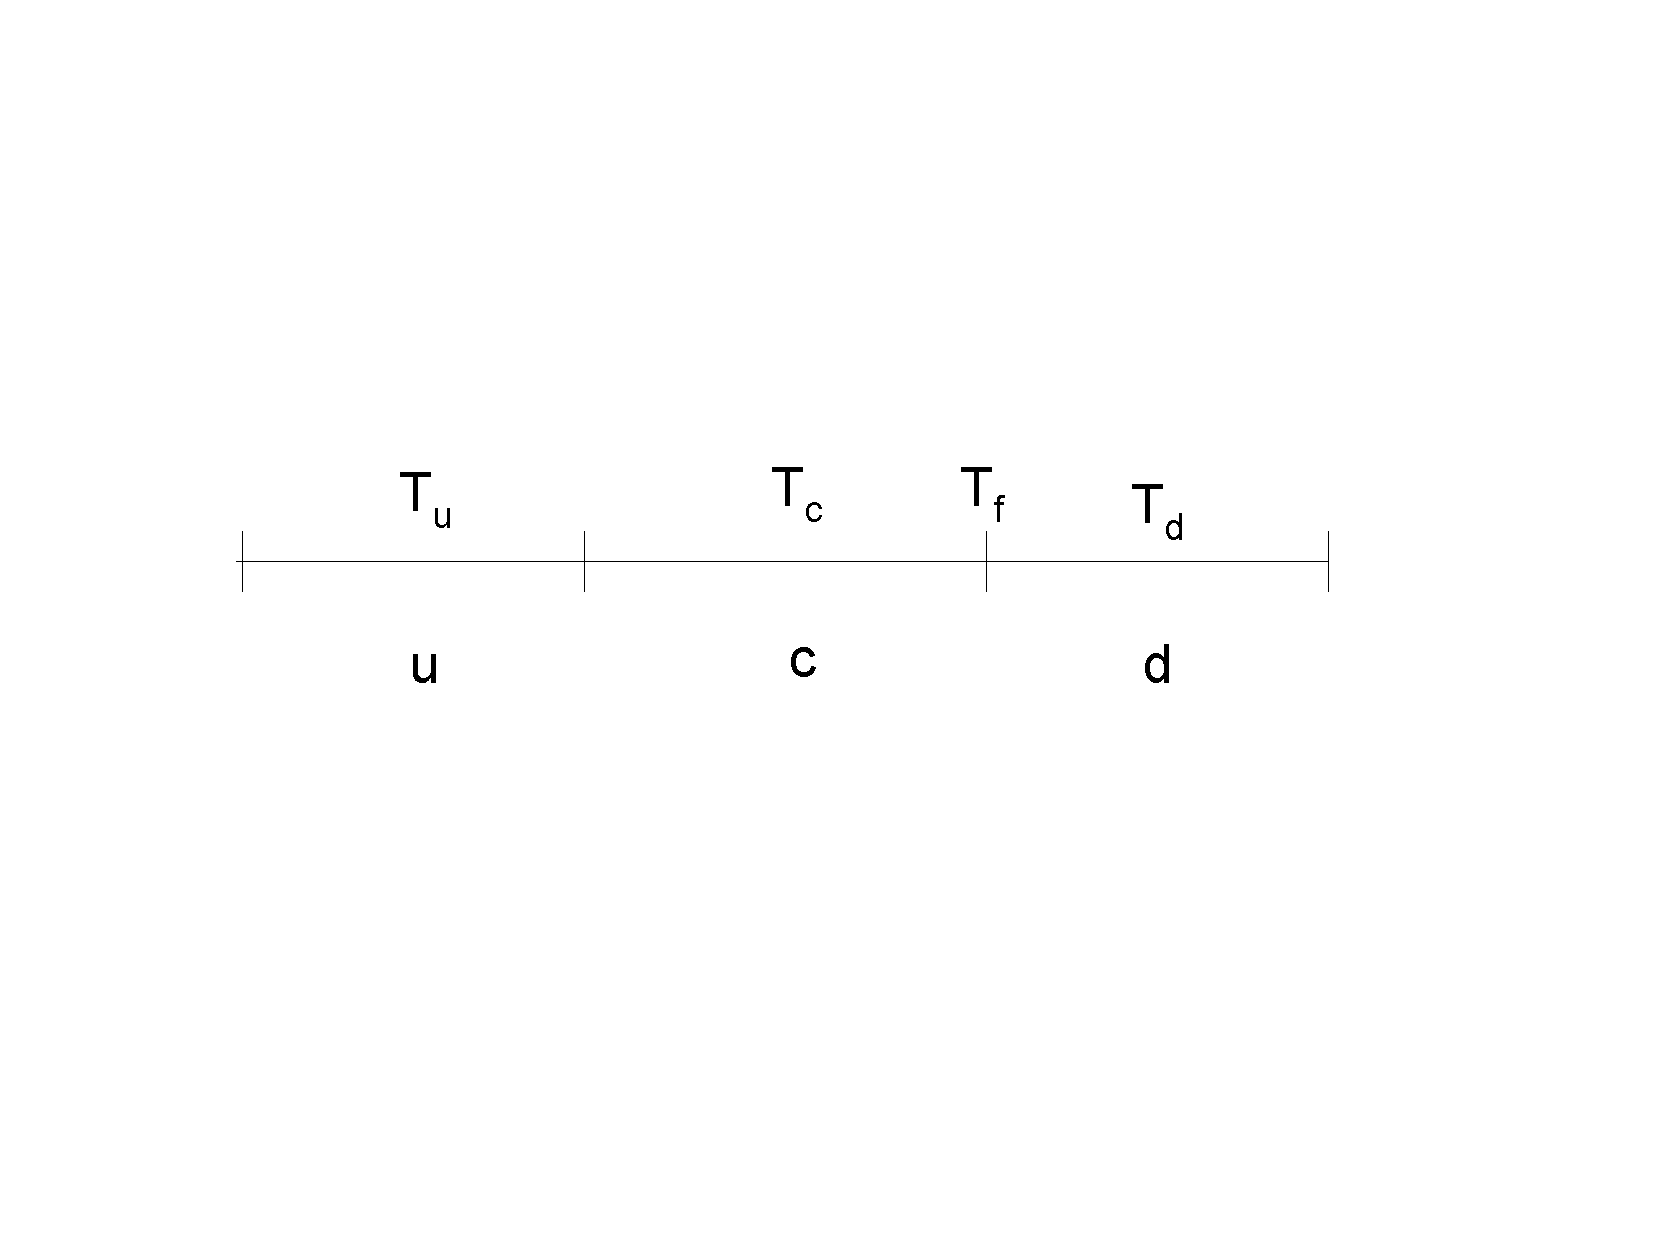
\includegraphics[width=15.0cm,height=10.cm]{./doc_figures/1D_FEM_CV}
\end{center}
\vspace{-5cm}}
\caption{1-D finite element showing CV's {\it u, c, d} and face {\it f}.}
\label{fem_cv_represent_a}
\end{figure}

%%%==============================================
%%% FIGURE 01 - Discretization 
%%%==============================================
\begin{figure}[H]
\vbox{
\begin{center}
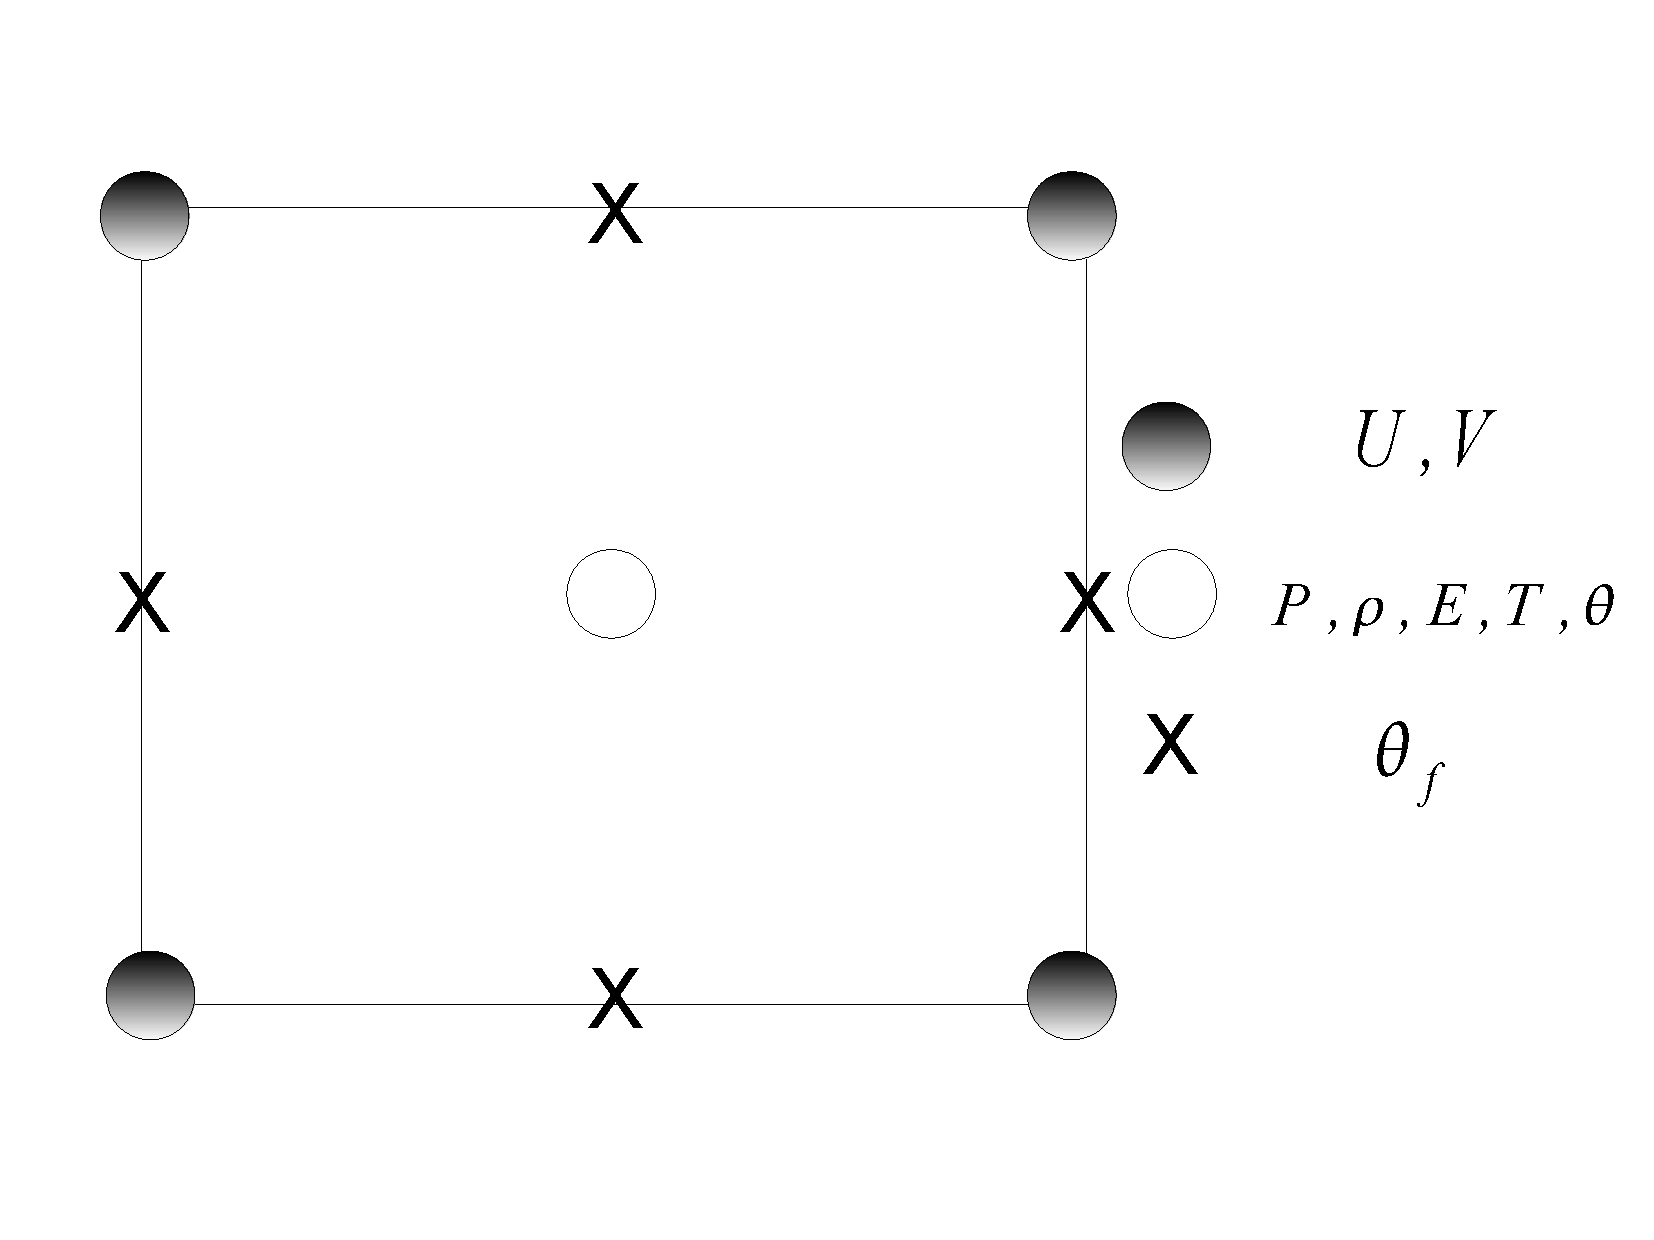
\includegraphics[width=9.0cm,height=7.0cm]{./doc_figures/FEM_elem}
\end{center}
\vspace{-1cm}}
\caption{Finite element used to discretize the fluids equations.  The central position of key solution variables are indicated here.}
\label{fem_cv_represent_b}
\end{figure}

Suppose that each element $i$ of our finite element mesh has a control volume and a solution variable $\hat T_i$ associated with it. Then the FEM solution $\widehat{T}$ is related to the CV solution \textit{T} by
%%
%% - begin displaymath
%%
\begin{displaymath}
\int_{V} N_{i} (\widehat{T} - T) \,d V = 0, \quad
\forall i\in \{1,2,...,{\mathcal N}\}
\end{displaymath}
in which $N_{i}$ is the finite element basis function associated with node \textit{i} and $M_{i}$ is the finite volume basis function (top hat function), which in our formulation is unity over element $i$ and zero elsewhere. In addition, the FEM representation of \textit{T} is given by $\widehat{T} = \sum\limits_{j=1}^{\mathcal{N}} N_{j} \widehat{T}_{j}$. Thus,
%%
%% - begin equation
%%
\begin{equation}
B \underline{\widehat{T}} = Q \underline{T}
\label{BQ}
\end{equation}
with $B = \int\limits_{V} N_{i} N_{j} \,d V$ and $Q =\int\limits_{V} N_{i} M_{j} \,d V$. The vectors $\underline{\widehat{T}} = \left(\widehat{T}_{1}, \widehat{T}_{2}, \ldots, \widehat{T}_{\mathcal{N}} \right)^{T}$, $\underline{T} =\left(T_{1}, T_{2}, \ldots,  T_\mathcal{M} \right)^{T}$ contain the unknown finite element and CV values of $T$, respectively. Both matrices \textit{B} and \textit{Q} have sparse structure.

%%
%%********************************************************
%%********************************************************
%%

\subsection{Extrema detecting}

To determine where to apply first order instead of high order fluxes, extremas must be detected and if there is a smooth transition between the high and low order fluxes, the closeness to an extrema must be quantified. This is achieved using the normal variable diagram NVD approach \index{\fluidity Module! Transport methods! NVD approach} as follows. Suppose $T_{u}, T_{c}, T_{d}$ are ordered consecutively and $T_{f}$ is the face value between CV's \textit{c} and \textit{d} (see Fig. \ref{fem_cv_represent_a}). In which case for a monotonic solution
%%
%% - begin equation
%%
\begin{equation}
\mathcal{T}_{f} = \frac{T_{f} - T_{u}}{T_{d} - T_{u}}  \in [0,1]
\label{p4a}
\end{equation}
where $\mathcal{T}_{f}$ is the non-dimensional high order face value.  The non-dimensional upwind face value is
\begin{equation}
\mathcal{T}_{c} = \frac{T_{c} - T_{u}}{T_{d} - T_{u}}
\label{p4b}
\end{equation}
The idea is to obtain a linear combination $\widetilde{\mathcal{T}}_{f}$ of $\mathcal{T}_{f}$ and $\mathcal{T}_{c}$ such that $\widetilde{\mathcal{T}}_{f}$ equals $\mathcal{T}_{c}$ when there is a local extrema ($\mathcal{T}_{c} \notin [0,1]$ and the scheme becomes first order) and $\widetilde{\mathcal{T}}_{f}$ moves smoothly between this and the high order flux $\mathcal{T}_{f}$ according to the curve shown on the NVD diagram \citep[see][]{gomes_2008}. $\widetilde{T}_{f}$ is calculated from
\begin{equation}
\widetilde{\mathcal{T}}_{f} = \frac{\widetilde{T}_{f} - T_{u}}{T_{d} - T_{u}}.
\label{2.1a}
\end{equation}
The flux limited solution is
\begin{equation}
\widetilde{T}_{f} = \widetilde{\mathcal{T}}_{f} (T_{d} - T_{u}) + T_{u}.
\label{2.1b}
\end{equation}
$\widetilde{\mathcal{T}}_{f}$ (see Fig. \ref{fem_cv_represent_a}) in this equation is calculated from:% (see Fig. \ref{nvddiag}):
\begin{equation}
\widetilde{\mathcal{T}}_{f} =
  \begin{cases}
    \min \{ \widetilde{\gamma} {\cal T}_{c}, \max \{ 0, {\cal T}_f\} \}, & \text{if} \
    \mathcal{T}_{c} \in (0,1); \\
    \mathcal{T}_{f},  & \text{otherwise},
  \end{cases}
\label{2.1c}
\end{equation}
with $\widetilde{\gamma} = 2.0$. Thus at an extrema the first order non-oscillatory method will be applied.  The curve $\mathcal{T}_{f} = 2\mathcal{T}_{c}$ has been chosen as an upper bound on $\widetilde{\mathcal{T}}_{f}$ as this corresponds to a TVD condition in 1-D \index{\fluidity Module! Transport methods! TVD condition} with equally spaced cells/elements \citep[see][]{hirsch_1990}.  One can use larger values of the gradient $\widetilde{\gamma}$ but convergence of the resulting non-linear iteration can suffer.  However, a larger gradient can help maintain sharper features in the solution, as reported by \citet{jasak_1999}.  They recommend the use of a gradient of 6 ($\widetilde{\gamma} = 6$, Eqn. \ref{2.1c}), they also recommend that the gradient should not be greater than 10 and not less than 2.  \citet{piperno_1998} explain some useful criteria for constructing limiting functions.  In addition, they use a maximum NVD curve with C$^{1}$ continuity, which is claimed to improve convergence, and use a quotient of gradients as opposed to the quotient of differences used here in Eqns. \ref{p4a}-\ref{2.1a}. 


\subsection{Extrema detection in multi-dimensions and isotropic limiting}

When integrating over a face of a CV in multi-dimensions we denote the cell from which the velocity is coming from as \textit{c} and the cell to which the velocity is pointing to \textit{d} (as in the previous section) with corresponding solution variables of $T_{c}$ and $T_{d}$ and the far field upwind value $T_{u}$. The value of $T_{u}$, for multi-dimensional  problems, is not well defined and thus it is this the the remainder of this section concerns.

The surface integral in Eqn. \ref{a} is calculated by summing the surface integrals over each face of CV \textit{i}. This face surface integral is evaluated using Gaussian quadrature. The values of $\widehat{T}$ at the Gauss points are limited using the NVD approach as described in the previous section, so that no new extrema are introduced into the solution \textit{T}. This is achieved by considering the velocity at the Gauss points on the face of an element. Out of the two CV's sharing this face, the CV from which the velocity is pointing away from is chosen as CV $c$ and the other CV denoted as \text{d}.


The minimum and maximum value of $T$ of the six CV's in 3-D and four CV's in 2-D, sharing a face with (less than this if near a boundary) with CV $c$ and CV \textit{c} itself, which we denote as $T_{\min}$ and $T_{\max}$. A non-dimensional temperature is then obtained at the Gaussisn integration point from the high order temperature $T_{f}$, via Eqn. \ref{2.1b} with the value of $T_{u}$ obtained from
%%
%% - begin equation
%%
\begin{equation}
T_{u} =
\begin{cases}
   T_{\max}, & \text{if} \ T_{d} \leq T_{c}; \\
   T_{\min}, & \text{if} \ T_{d} > T_{c}.
\end{cases}
\label{rr}
\end{equation}

This then allows the flux limiting, Eqns. \ref{2.1a}-\ref{2.1c} to be applied. This approach is the recommended isotropic limiting method.  One can amend $T_{\max}$ and $T_{\min}$ to take into account variable grid resolution using instead:

\begin{equation}
T_u = T_c + \frac{\Delta_{cd}}{\Delta_{uc}} ( T_{\max} - T_c) 
\end{equation}
\noindent
or\\ 
\begin{equation}
T_u = T_c + \frac{\Delta_{cd}}{\Delta_{uc}} ( T_{\min} - T_c) 
\end{equation}
depending on the criteria in Eqn. \ref{rr}. $\Delta_{cd}$ is proportional to the distance between the CV cells $c$ and $d$ and $\Delta_{uc}$ is proportional to the distance between the CV cells $u$ and $c$. For example, $\Delta_{cd} = \frac{1}{2}(V_c + V_d)$ and  $\Delta_{uc} = \frac{1}{2}(V_{max} + V_c)$ or  $\Delta_{uc} = \frac{1}{2}(V_{min} + V_c)$ again  depending on criteria expressed by Eqn. \ref{rr}. $V_{min}$ is the volume of  the cell surrounding CV $c$ that has a minimum value of $T$,  $V_{max}$ is the volume of  the cell surrounding CV $c$ that has a maximum value of $T$, and $V_c$ and $V_d$ are the volumes of cells $c$ and $d$.  The alternative would be to use geometrical distances to define $\Delta_{cd}$ and $\Delta_{uc}$. 

The most relaxed form of limiting is obtained from
\begin{equation}
\mathcal{T}_{f} = \frac{T_{f} - T_{\min}}{T_{\max} - T_{\min}}
\label{r}
\end{equation}
\noindent
and
\begin{equation}
\mathcal{T}_{c} = \frac{T_{c} - T_{\min}}{T_{\max} - T_{\min}}
\label{r_p}
\end{equation}
which results in useful bounded schemes. Moreover the scheme defined by Eqns. \ref{r} and \ref{r_p} introduce less dissipation than other bounded
schemes. These two flux limiting methods will prevent any new extrema from forming, however for a given direction new extrema can form along this direction results in oscillations in the solution. However, by choosing a control volume value in the upwind direction from face $f$ and just upwind from CV $c$ then this problem can be circumvented.


\subsection{Time Discretization} \label{time_discretisation}\index{\fluidity Module! Transport methods ! Time discretisation}
A new time discretisation method is developed here. When high order discretization in time 
is sought then the method is based on Crank-Nicholson time stepping.  The Crank-Nicholson method was chosen, because it has the simplicity of a two level time stepping method, is unconditionally stable and second order accurate. 
However, if interface capturing then the scheme is based on explicit forward Euler time stepping which 
introduces negative dissipation and is thus a compressive scheme which helps maintain sharp interfaces. 
Moreover, the use of time steps of the order of the grid Courant number and above can result in numerical oscillations and unphysical solutions. Thus a parameter $\theta$ is introduced, in which $\theta$ = 0 corresponds to the forward Euler time stepping method, 
$\theta$ = $\frac{1}{2}$ corresponds to the Crank-Nicholson time stepping method and $\theta$ = 1 backward-Euler.
Then using Eqns. \ref{CV1} and \ref{a} the time stepping for Eqn. \ref{traneq} takes the form:
%%
%% - begin equation
%%
\begin{eqnarray}
\int M_i \left( \frac{T_{i}^{n+1} -T_{i}^{n}}{\Delta t} - s \right) \,dV= \nonumber \\
\int_{\Gamma_{CV_{i}}} \left[\theta\left(\mathbf{a}^{n+1}\cdot \mathbf{n} \widetilde{T}^{n+1}
+\mathbf{n}\cdot k^{n+1}\nabla \widetilde{T}^{n+1}   \right)+\left(1-\theta\right)\left(\mathbf{a}^{n}\cdot \mathbf{n} \widetilde{T}^{n}
+\mathbf{n}\cdot k^{n}\nabla \widetilde{T}^{n}
 \right)  \right]d\Gamma
 \label{theta}
\end{eqnarray}
For each time step a value of $\theta$ is calculated at each CV face based on the satisfaction of a TVD criteria. In 1-D, assuming the flux limiting values of the flux at the $i-{\frac{1}{2}}$ and $i+{\frac{1}{2}}$ boundaries (see Fig. \ref{fem_cv_represent_c}) are $h^{n}_{i-{\frac{1}{2}}}$ and $h^{n}_{i+{\frac{1}{2}}}$ at time level \textit{n},  the time discretization becomes:
%%
%% - begin equation
%%
\begin{equation}
\Delta x_i \left( \frac{T_{i}^{n+1} - T_{i}^{n}}{\Delta t} \right)
= \theta_{i-\frac{1}{2}}^{n+{\frac{1}{2}}} h_{i-\frac{1}{2}}^{n+1}
+(1-\theta_{i-\frac{1}{2}}^{n+{\frac{1}{2}}}) h_{i-\frac{1}{2}}^n
-\theta_{i+\frac{1}{2}}^{n+\frac{1}{2}} h_{i+\frac{1}{2}}^{n+1}
-(1-\theta_{i+\frac{1}{2}}^{n+\frac{1}{2}}) h_{i+\frac{1}{2}}^n
\label{thetareq1}
\end{equation}
with
%%
%% - begin displaymath
%%
\begin{displaymath}
h_{i-\frac{1}{2}}^{n} = a_{i-\frac{1}{2}}^{n}
T_{i-\frac{1}{2}}^{n}
 +k_{i-\frac{1}{2}}^n \frac{\partial
T^n}{\partial x}\left\vert_{i-\frac{1}{2}}\right.
\end{displaymath}

%%%==============================================
%%% FIGURE 01 - Discretization issues
%%%==============================================
\begin{figure}[H]
\vbox{
\begin{center}
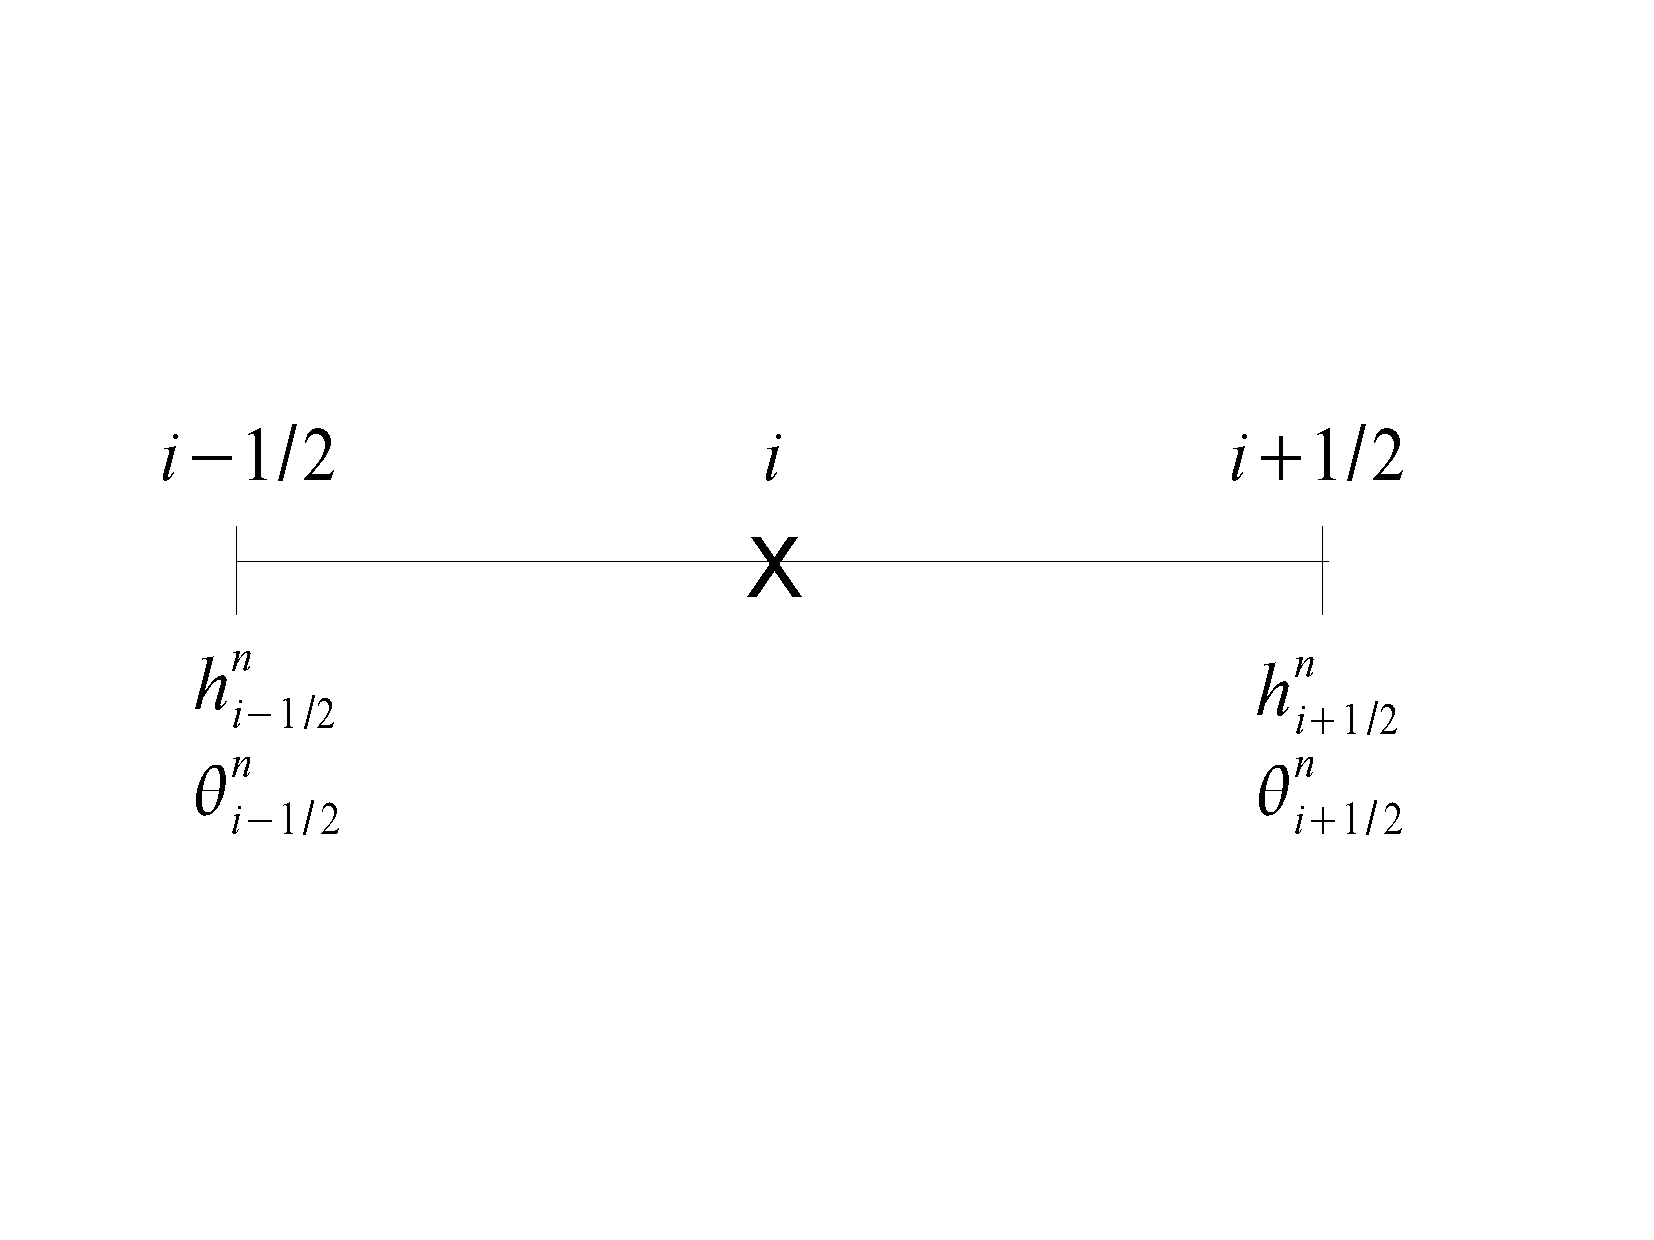
\includegraphics[width=10.0cm,height=7.5cm]{./doc_figures/FEM_elem2}
\end{center}
\vspace{-3.cm}}
\caption{Positioning of variables in and on the boundary of CV {\it i}.}
\label{fem_cv_represent_c}
\end{figure}
%%%==============================================
%%%                 FIGURE 01 
%%%==============================================



%%%==============================================
%%%             FIGURE - P1DGP2
%%%==============================================
\begin{figure}[H]
\vbox{
\hbox{
\hspace{0.cm}
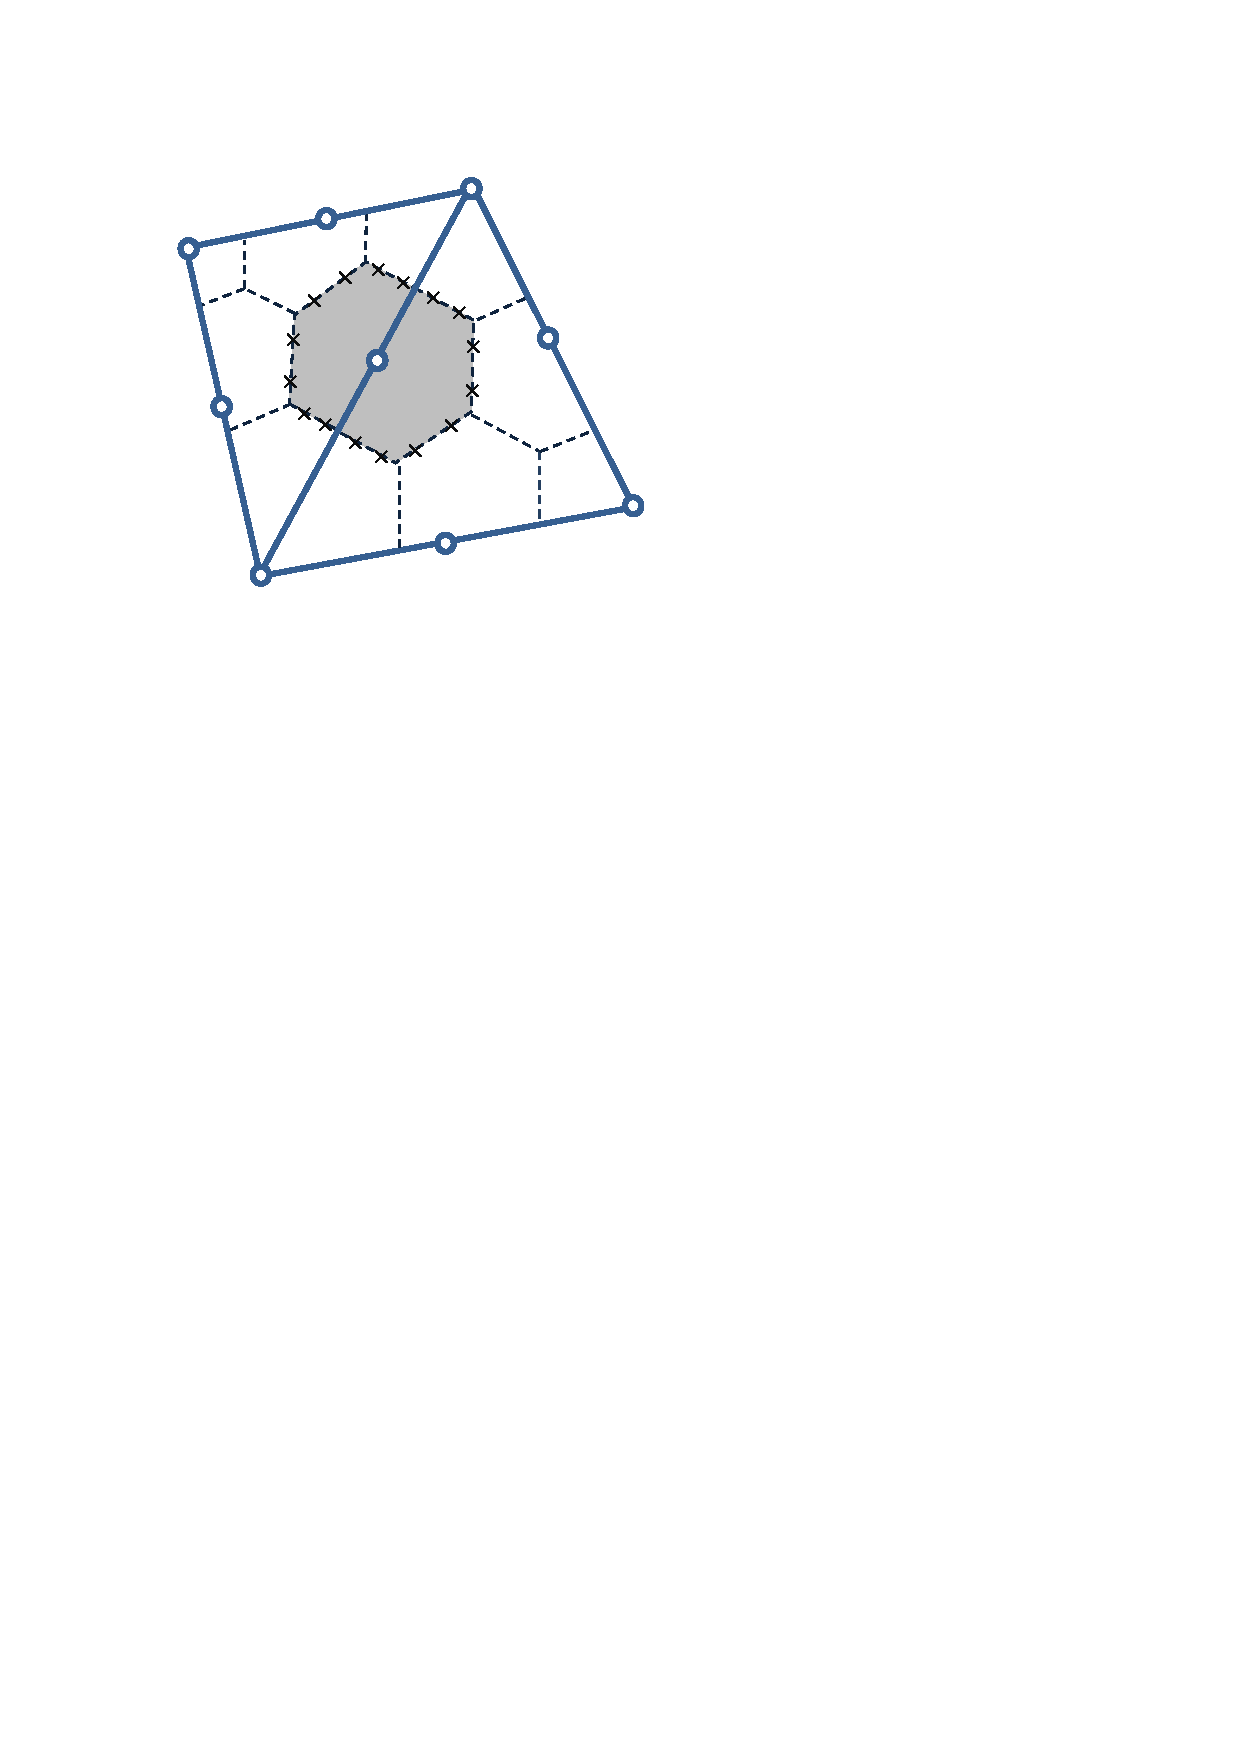
\includegraphics[width=7.0cm,height=7.cm]{./doc_figures/p1dg-p2-elepic}
\hspace{-0.cm}
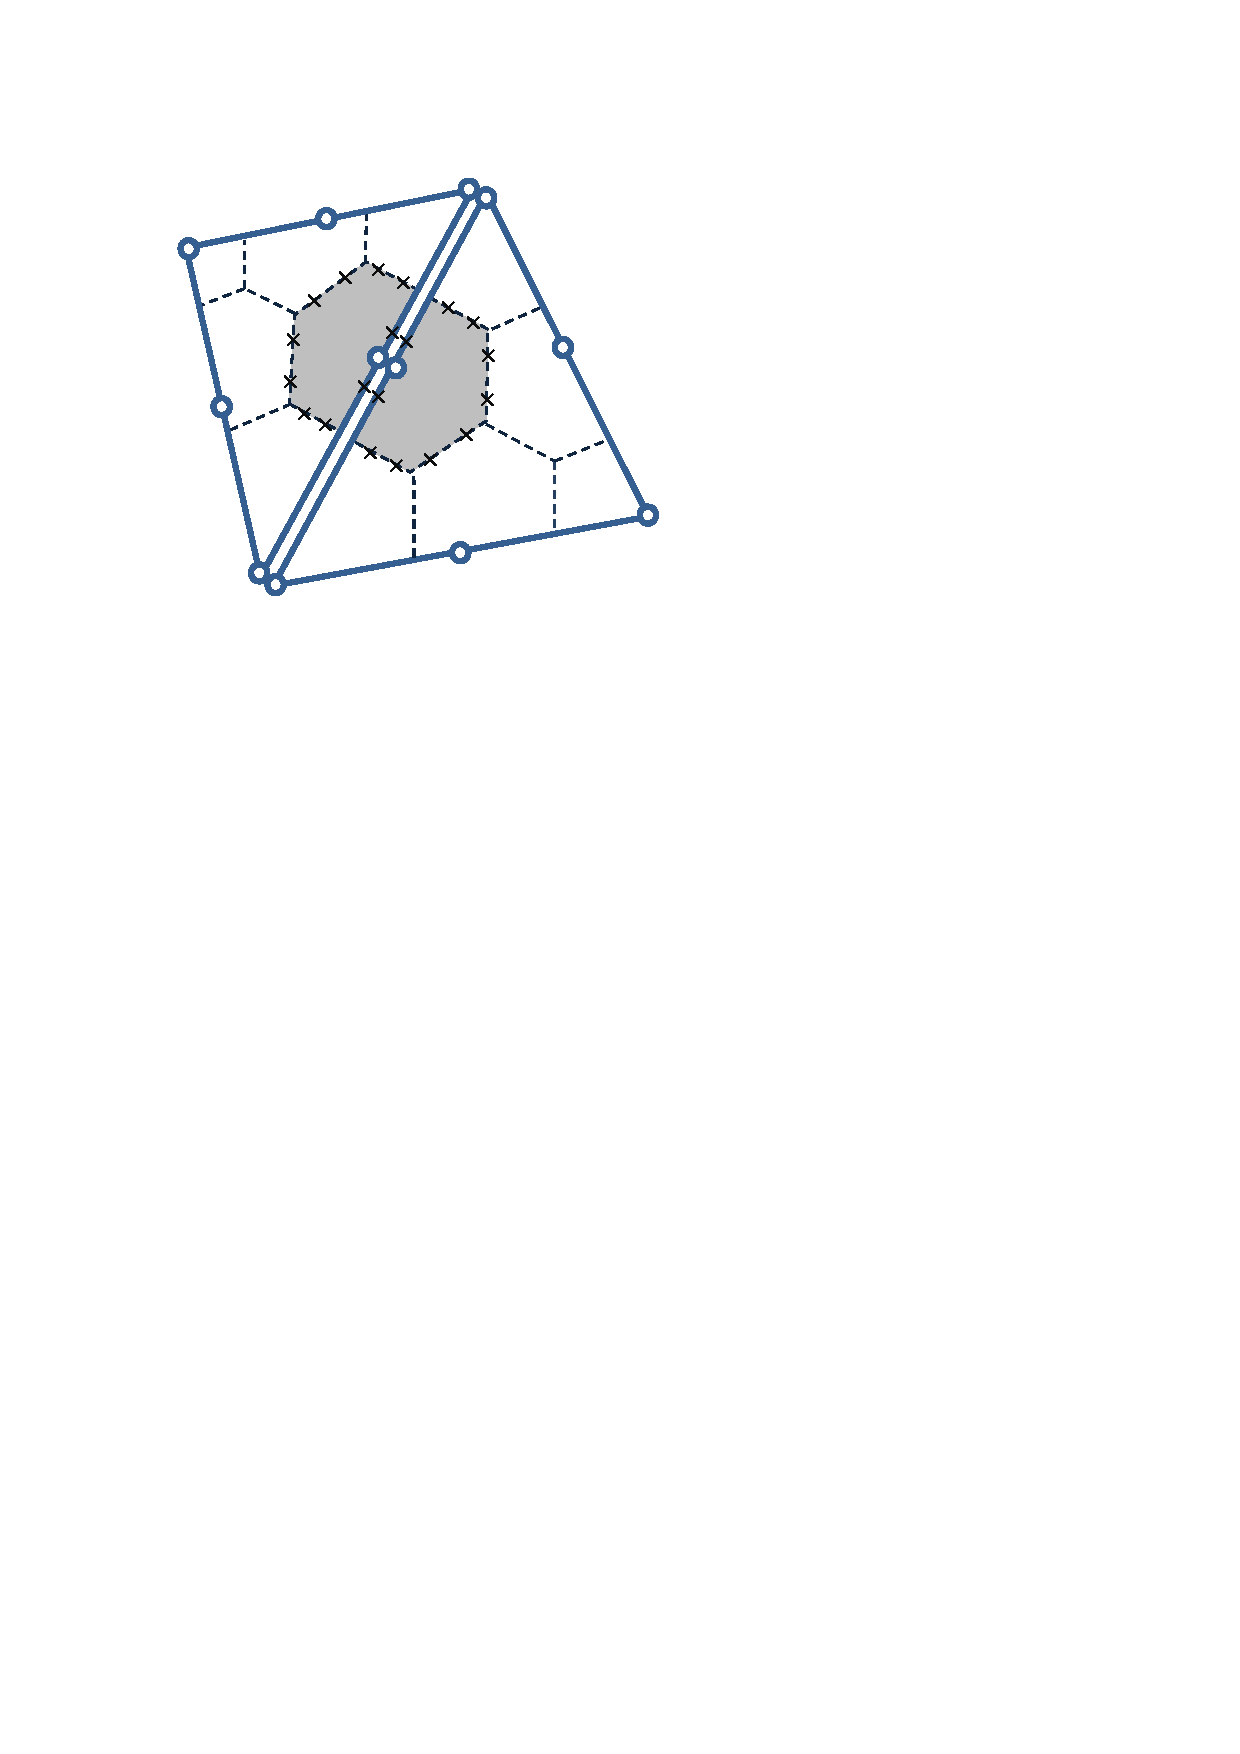
\includegraphics[width=7.0cm,height=7.cm]{./doc_figures/p1dg-p2-dgsat-elepic}
}
\vspace{-0.cm}
\hbox{\hspace{4.cm}(a) \hspace{6.5cm}(b)}
\vspace{-0.cm}}
\label{p1dgp2_ele-dgsat_pics}
\caption{2D finite element containing control volumes is shown. The circles represent the underlying finite element nodes and dashed lines the boundaries of the control volumes. The crosses show typical quadrature points used to integrate around the control volumes. (a) Continuous pressure and tracer solution between the elements. (b) Discontinuous pressure and tracer between elements.  }
\end{figure}
%%%==============================================
%%%             FIGURE - P1DGP2
%%%==============================================

\noindent
$\Delta x_{i}$ is the width of the $i^{th}$ CV and $\theta_{i+\frac{1}{2}}^{n+\frac{1}{2}}$ is the value of $\theta$ associated with face $i+\frac{1}{2}$ and the time step from time level $n$ to $n+1$.  The representation of $k_{i-\frac{1}{2}}^n \frac{\partial T^n}{\partial x}\vert_{i-\frac{1}{2}}$ is considered in a following section.% a simple example of which is $\frac{T_i^{n+1}-T_{i-1}^n}{\Delta x}$ in which $\Delta x$ is the size of the control volumes.  

Re-arranging Eqn. \ref{thetareq1}:
%%
%% - begin displaymath
%%
\begin{eqnarray}
\left( \Delta x_i - \Delta t \frac{\left[
-\widehat{\theta}_{i-\frac{1}{2}}^{n+\frac{1}{2}}(
-h_{i-\frac{1}{2}}^{n+1}+h_{i-\frac{1}{2}}^{n})
+\widehat{\theta}_{i+\frac{1}{2}}^{n+\frac{1}{2}}(
-h_{i+\frac{1}{2}}^{n+1}+h_{i+\frac{1}{2}}^{n}) \right]}
{T_i^{n+1}-T_i^n} \right)
\left(\frac{T_i^{n+1} - T_i^n}{\Delta t} \right) =\nonumber\\
h_{i-\frac{1}{2}}^{n+1}-h_{i+\frac{1}{2}}^{n+1}\nonumber
\end{eqnarray}
with
%%
%% - begin displaymath
%%
\begin{displaymath}
\widehat{\theta}_{i-\frac{1}{2}}^{n+\frac{1}{2}}  = 1-\theta_{i-\frac{1}{2}}^{n+\frac{1}{2}}.
\end{displaymath}
Now since backward Euler time stepping is TVD in the same way that first order upwind scheme is spatially, a positive definite mass matrix is a sufficient condition for the backward Euler scheme above to be TVD \citep[see][]{hirsch_1990}\index{\fluidity Module! Transport methods! TVD condition}.  Thus the diagonal mass matrix (the term in brackets) must be non-negative, after re-arranging this requirement becomes
%%
%% - begin displaymath
%%
\begin{displaymath}
\frac{\Delta t}{\Delta x_{i}\left(T_i^{n+1} - T_i^{n}\right)} \left[ \widehat{\theta}_{i-\frac{1}{2}}^{n+\frac{1}{2}}\left(h_{i-\frac{1}{2}}^{n} - h_{i-\frac{1}{2}}^{n+1}\right)-\hat\theta_{i+\frac{1}{2}}^{n+\frac{1}{2}}\left(h_{i+\frac{1}{2}}^{n}-h_{i+\frac{1}{2}}^{n+1}\right) \right] \leq 1
\end{displaymath}
and thus
%%
%% - begin displaymath
%%
\begin{displaymath}
\left(\widehat{\theta}_{i-\frac{1}{2}}^{n+\frac{1}{2}}
p_{i-\frac{1}{2}}^{n+\frac{1}{2}}
-\widehat{\theta}_{i+\frac{1}{2}}^{n+\frac{1}{2}}
q_{i+\frac{1}{2}}^{n+\frac{1}{2}} \right) \leq 1
\end{displaymath}
with
%%
%% - begin displaymath
%%
\begin{displaymath}
p_{i-\frac{1}{2}}^{n+\frac{1}{2}} = \left( \frac{h_{i-\frac{1}{2}}^{n}
- h_{i-\frac{1}{2}}^{n+1}}{T^{n+1}_{i} - T_{i}^{n}} \right)
\frac{\Delta t}{\Delta x_{i}}  \quad \text{and} \quad
q_{i+\frac{1}{2}}^{n+\frac{1}{2}} = \left(
\frac{h_{i+\frac{1}{2}}^n-h_{i+\frac{1}{2}}^{n+1}}{T^{n+1}_{i} - T_{i}^{n}}
\right) \frac{\Delta t}{\Delta x_{i}}
\end{displaymath}
which is satisfied if
%%
%% - begin equation
%%
\begin{equation}
- \widehat{\theta}_{i-\frac{1}{2}}^{n+\frac{1}{2}}
p_{i-\frac{1}{2}}^{n+\frac{1}{2}} \leq \frac{1}{2} \quad \text{and} \quad
- \widehat{\theta}_{i-\frac{1}{2}}^{n+\frac{1}{2}}
q_{i-\frac{1}{2}}^{n+\frac{1}{2}} \geq
\frac{1}{2}
\label{half}
\end{equation}
Thus to make the value of $\theta_{i-\frac{1}{2}}^{n+\frac{1}{2}}= 1 - \widehat{\theta}_{i-\frac{1}{2}}^{n+\frac{1}{2}}$ as close to $\theta_{aim}$ as possible we choose
%%
%% - begin displaymath
%%
\begin{displaymath}
\theta_{i-\frac{1}{2}}^{n+\frac{1}{2}} = \max \left\{ \theta_{aim},
1 - \beta \min \left\{ \left|\frac{1}{p_{i-\frac{1}{2}}^{n+\frac{1}{2}}}\right|,
\left|\frac{1}{q_{i-\frac{1}{2}}^{n+\frac{1}{2}}} \right| \right\} \right\}
\end{displaymath}
with $\beta=\frac{1}{2}$ and $\theta_{aim}=\frac{1}{2}$ is the base scheme and is the 
high order accurate Crank Nickolson scheme and $\theta_{aim}=0$ if it is forward Euler time 
stepping which is favoured when interface capturing. 

\subsection{Multi-dimensional temporal limiting}
\label{multidimtemplim}

The high resolution $\theta$ method can be extended to multi-dimensions by replacing $h_{i-\frac{1}{2}}^{n}$ with the integral of $\tilde{h}_{f}^{n}$ over face \textit{f} and $\Delta x_{i}$ replaced by the volume $L_{i}$ (contribution from diagonal mass matrix) of the $i^{th}$ CV. Using similar arguments to the 1-D case the following expression for $\theta_f^{n+\frac{1}{2}}$ of face \textit{f} is obtained:
%%
%% - begin equation
%%
\begin{equation}
\theta_f^{n+\frac{1}{2}}=\max \left\{ \theta_{aim}, 1 - \beta \min\left\{
\left|\frac{1}{p_{f}^{n+\frac{1}{2}}}\right|,\left|
\frac{1}{q_{f}^{n+\frac{1}{2}}} \right| \right\} \right\}
\label{thet1}
\end{equation}
with
%%
%% - begin equation
%%
\begin{equation}
p_f^{n+\frac{1}{2}} =
\frac{g_f^{n+\frac{1}{2}}\Delta t}{(T^{n+1}_{c} - T_{c}^{n}) L_{c}}
\quad \text{and} \quad q_f^{n+\frac{1}{2}} =
\frac{g_f^{n+\frac{1}{2}}\Delta t}{(T^{n+1}_{d} - T_{d}^{n}) L_{d}}
\label{thet2}
\end{equation}
and
%%
%% - begin equation
%%
\begin{equation}
g_f^{n+\frac{1}{2}}= (\tilde{h}_{f}^{n} - \tilde{h}_f^{n+1})
\label{gf}
\end{equation}
CV's \textit{c} and \textit{d} in these equations refer to the two CV's that are adjacent to face \textit{f}, (see Fig. \ref{fem_cv_represent_b}). Extensions of this method to differential equations with time-dependent terms like $\frac{\partial \rho T}{\partial t}$ are realized by replacing, in Eqn. \ref{thet2}, $T_j^n$ and $T_j^{n+1}$ by $T_{j}^{n} \rho_{j}^{n}$ and $T_{j}^{n+1} \rho_j^{n+1}$ respectively for $j = c$ and $j = d$.


\subsection{Control Volume Diffusion Discretization}\label{section_diff_discretisation}\index{\fluidity ! Transport methods ! Diffusion discretisation}

The high resolution $\theta$ method can also be used with diffusion by adding to $g_{f}^{n+\frac{1}{2}}$ in Eqn. \ref{gf} the flux limited discretized contribution, integrated along face $i-\frac{1}{2}$.
In 1-D this might lead to
%%
%% - begin displaymath
%%
\begin{displaymath}
g_{i-\frac{1}{2}}^{n+\frac{1}{2}} = h_{i-\frac{1}{2}}^n-h_{i-\frac{1}{2}}^{n+1}
= a_{i-\frac{1}{2}}^n T_{i-\frac{1}{2}}^n -
a_{i-\frac{1}{2}}^{n+1} T_{i-\frac{1}{2}}^{n+1} + \kappa \left(
\frac{T_{i}^n-T_{i-1}^n}{\frac{1}{2}(\Delta x_{i-1}+\Delta x_i )}
- \frac{T_{i}^{n+1}-T_{i-1}^{n+1}}{\frac{1}{2}(\Delta
x_{i-1}+\Delta x_i )}\right)
\end{displaymath}
in which $\kappa$ is the diffusion coefficient. In multi-dimensions this becomes
%%
%% - begin displaymath
%%
\begin{displaymath}
g_{f}^{n+\frac{1}{2}} = \tilde h_{f}^n-\tilde h_{f}^{n+1}
\end{displaymath}
in which
%%
%% - begin displaymath
%%
\begin{equation}
\tilde{h}_{f}^{n} = \int_{\Gamma_f} \left( a \cdot n T^{n}
+ \kappa \frac{\partial T^n}{\partial n_x} \right) \,d\Gamma
\label{16a}
\end{equation}
where $n_x$ is the normal to the control volume. Now if the underlying scheme that calculates $\frac{\partial T^n}{\partial n_x}$ is non-oscillatory then the advection-diffusion scheme will be non-oscillatory. A simple example of this is
%%
%% - begin displaymath
%%
\begin{displaymath}
\frac{\partial T^n}{\partial n_x}\Big\vert_{no_f} = \frac{\partial T^n}{\partial n_x} \Big\vert_{f} = \frac{T_{c}^{n} - T_{d}^{n}}{\Delta x_{f}}
\end{displaymath}
in which, as before, the subscripts denote cells that share face \textit{f} (see Fig. \ref{fem_cv_represent_b}), $\Delta x_{f}$ is a measure of the component of distance between the centres of the CV's \textit{c} and \textit{d} in the normal direction to face $f$. This equation also serves as a definition of $\frac{\partial T^{n}}{\partial n_x}\vert_{no_f}$. The accuracy of this approximation can be improved, but once again non-linearity must be used to ensure boundedness of the scheme. Suppose the underlying non-oscillatory approximation to $\frac{\partial T}{\partial n_x}$ is $\frac{\partial T^n}{\partial n_x}\vert_{no_f}$ then any positive multiple of this will result in a bounded scheme and as such the TVD condition is
%%
%% - begin displaymath
%%
\begin{displaymath}
{\frac{\partial \widetilde{T}^{n}}{\partial n_x}\Big\vert_{f}
\frac{\partial T^{n}}{\partial n_x}\Big\vert_{no_f}} \geq 0
\end{displaymath}
The scheme is bounded if the high order limited derivative $\frac{\partial \widetilde{T}^{n}}{\partial n_x}\vert_{f}$ has the same sign as $\frac{\partial T^{n}}{\partial n_x}\vert_{no_f}$. However, to avoid difficulties with the non-linear convergence the derivative of $\frac{\partial \widetilde{T}^{n}}{\partial n_x}\vert_{f}$ from the high order approximation $\frac{\partial T^{n}}{\partial n_x}\vert_{f}$ is limited with
%%
%% - begin displaymath
%%
\begin{displaymath}
s_f \frac{\partial \widetilde{T}^{n}}{\partial n_x}\Big\vert_f
= \max \left\{ \gamma_2 s_f \frac{\partial T^{n}}{\partial n_x}\Big\vert_{no_f},
\min \left\{ s_f \frac{\partial T^{n}}{\partial n_x}\Big\vert_{f},
\gamma_{1} s_{f} \frac{\partial T^{n}}{\partial n_x}\Big\vert_{no_f} \right\}
\right\}
\end{displaymath}
with
%%
%% - begin displaymath
%%
\begin{displaymath}
\gamma_1 \geq 1 \geq \gamma_2 \geq 0
\end{displaymath}
and
%%
%% - begin displaymath
%%
\begin{displaymath}
s_f =
  \begin{cases}
     1 & \ \text{if} \ \frac{\partial T^n}{\partial n_x}\vert_{no_f} \geq 0; \\
    -1 & \ \text{otherwise} \
\end{cases}
\end{displaymath}
and $\frac{\partial T^{n}}{\partial n_x}\vert_{f}$ is the high order flux, which as with the advection scheme can be obtained from any high order representation of \textit{T}. The authors recommended that  $\gamma_{1} = 2, \ \ \gamma_2 = \frac{1}{2}$.  An example, using the FEM discretization would be to use the derivative along a face $f$ of a control volume from the FEM representation. For derivatives along the boundaries of an element one would use a finite element average of the derivative of the FEM representation of one element and the other sharing this face. 

In the case of a diffusion tensors ${\underline{\underline k}}$ this approach using the approximation: 

\begin{equation}
n\cdot {\underline{\underline k}} \nabla T = 
\min\left\{ \beta_{max}\frc{k_{norm}}{{\Delta x}_{f}} , \max\left\{ \beta_{min}\frc{k_{norm}}{{\Delta x}_{f}} , \left( \frc{k}{\Delta x} \right)_{\text{eff}} \right\} \right\}\left(T_{current}-T_{neighbour}\right)
\label{non-lin-diff}
\end{equation}
where 
%\help
\begin{equation}
\left( \frc{k}{\Delta x} \right)_{\text{eff}} =  
- \frc{1}{2} \frc{ n\cdot \left[ \left({\underline{\underline k}} \nabla T\right)_{neighbour} + \left({\underline{\underline k}} \nabla T\right)_{current} \right] }{T_{current}-T_{neighbour}} 
\label{non-lin-diff-eff} 
\end{equation}
and where $T_{current}$ is the solution in the current control volume and $T_{neighbour}$ is the solution in the neighbouring control volume between which the surface integral around the current control volume is being performed. $k_{norm}$ is the normal component of the tensor ${\underline{\underline k}}$ (normal to the boundary of the control volume) and is approximated here with $k_{norm} =n^T {\underline{\underline k}} n $.  It is obtained from equation 
\ref{non-lin-diff-eff} using the approximation:

\begin{equation}
\frac{k_{norm}}{{\Delta x}_f}=  
 \frac{ n\cdot {\underline{\underline k}} n (T_{current}-T_{neighbour})}{{\Delta x}_f(T_{current}-T_{neighbour})}
= \frac{n^T {\underline{\underline k}} n}{{\Delta x}_f}. 
\label{non-lin-diff-eff-approx} 
\end{equation}
${\Delta x}_f$ is the distance between the centre of the control volumes associated with $T_{current}$ and $T_{neighbour}$.  $\beta_{min}$ is the minimum fraction of the $\frac{k_{norm}}{{\Delta x}_{f}}$ to use $\left(\right.$we use $\beta_{min}=0.05\left.\right)$ and $\beta_{min}$ defines the upper bound on the value of the effective diffusivity $\left(\right.$we use $\beta_{max}=100\left.\right)$.  Without $\beta_{max}$ as $T_{current}$ and $T_{neighbour}$ become close this would make  $n\cdot {\underline{\underline k}} \nabla T$ large. 

There are three main advantages of the non-linear diffusion scheme above: 
\begin{enumerate}[1)]
\item the method does not introduce oscillations due to the high order representation of diffusion; 
\item the method is high order accurate most of the time; 
\item the method always result in a symmetric positive definite discretisation matrix (a property not shared with many high order diffusion control volume discretisations); 
\item the method results in a compact stencil and thus the resulting matricies are sparse. 
\end{enumerate}

Finally, it is noted that the FEM discretization using linear triangle, tetrahedra, rectangles or hexahedra of the diffusion term can also be bounded with restrictions on the distortion of the elements \citep[see][]{mizukami_1985}.


%%%==============================================
%%% FIGURE 01 - Discretization 
%%%==============================================
\begin{figure}[H]
\vbox{
\begin{center}
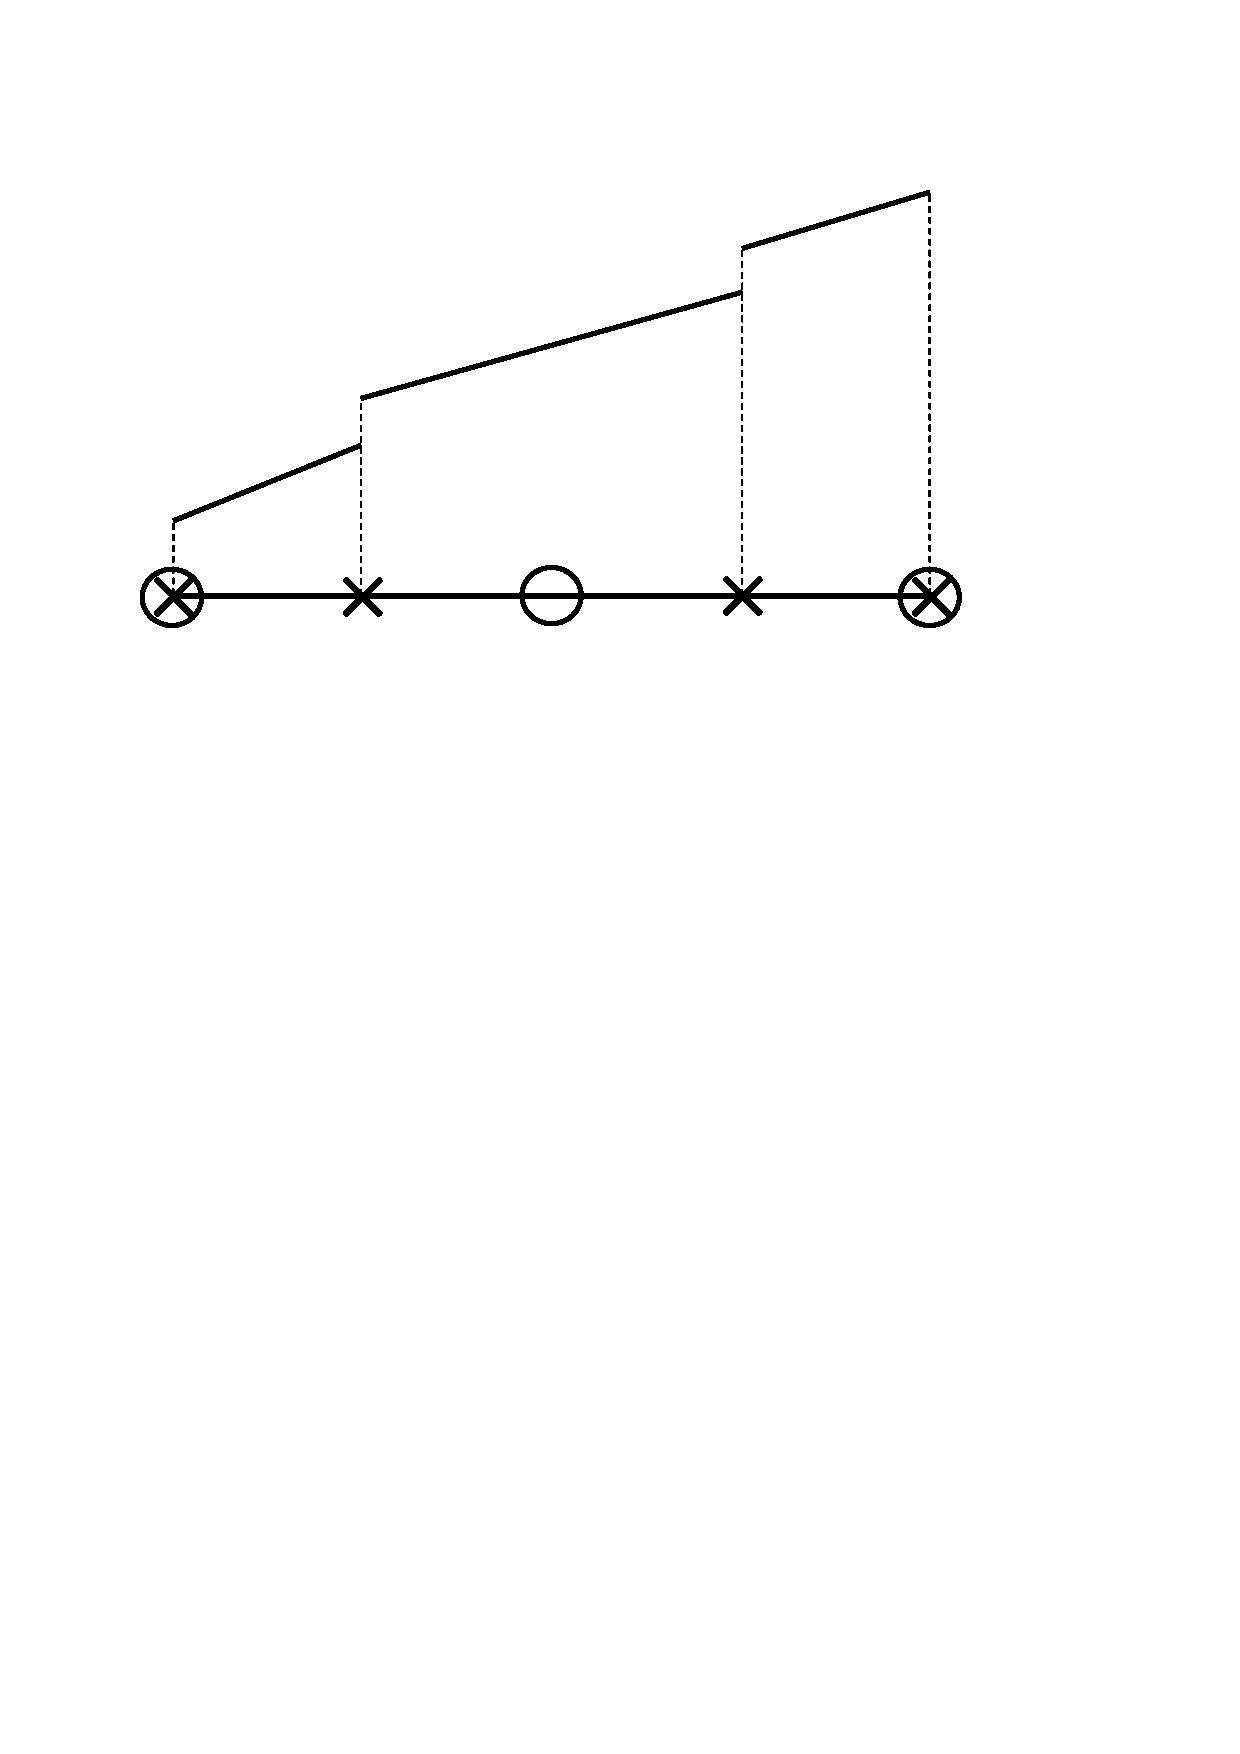
\includegraphics[width=15.0cm,height=10.0cm]{./doc_figures/CVFEM_1D}
\end{center}
\vspace{-1cm}
}
\caption{1-D finite element }
\label{fem_cv_represent_c}
\end{figure}

\subsection{Discontinuous Galerkin diffusion discretisation}

A simple form the DG discretised equations for diffusion is: 

\begin{equation}
\int_{V_{ele}} \nabla N_i {\underline {\underline k}} \nabla T_{fem}^n d\Omega 
+\int_{\Gamma_{ele}} N_i \alpha \left({T_{fem}^n}_{current}-{T_{fem}^n}_{neighbour} \right)  d\Gamma . 
\label{dg-variational-diff-low} 
\end{equation}
This has an underlying variational principle behind it. That is 
\begin{equation}
\frac{1}{2}
\int_{V_{ele}} \nabla T_{fem}^n {\underline {\underline k}} \nabla T_{fem}^n d\Omega 
+\frac{1}{2} 
\int_{\Gamma_{ele}} \alpha \left({{T_{fem}^n}_{current}-{T_{fem}^n}_{neighbour}} \right)^2 
d\Gamma, 
\label{variational-prin} 
\end{equation}
 and 
thus the discretised equations are guaranteed to be symmetric and positive definite as long as ${\underline {\underline k}}$ is sym-pos-def and scalar $\alpha$ is positive. The first term in Eqn. \ref{variational-prin} attempts to flatter the solution within an element and the latter surface integral attempts to produce continuity of the solution between elements. This is very similar to the way Robin boundary condition are typically applied using FEM: 
%%
%% - begin displaymath
%%
\begin{displaymath}
k \frac{\partial T^{n}}{\partial n} = \alpha (T - T_{0})
\end{displaymath}
can be applied directly in Eqn. \ref{16a}.

Testing with DG basis function $N_i$ and applying Greens theory to the diffusion term one obtains: 

\begin{equation}
\int_{V_{ele}} \nabla N_i \underline {\underline k} \nabla T_{fem}^n d\Omega 
-\int_{\Gamma_{ele}} N_i n\cdot \underline {\underline k} \nabla T_{fem}^n d\Gamma . 
\label{dg-variational-diff-high} 
\end{equation}
If one can turn this into the same form as Eqn. \ref{dg-variational-diff-low} (with a suitable chosen $\alpha$) then the stencil will be very compact and the method of evaluating the diffusion term for DG will have the same advantages as for CV as listed in Section \ref{section_diff_discretisation}.  The first term in Eqn. \ref{dg-variational-diff-high} is formed simply by placing  $T_{fem}^n=\sum_j Q_j {T_{fem}^n}_j$ into this equation. However, the term $n\cdot \underline {\underline k} \nabla T_{fem}^n $ is approximated as described in the next section from derivatives both sides of the element interface. That is the diffusion operator between elements is formed in the same manner as for the control volume discretisation using:
\begin{equation}
\left( \frac{k}{\Delta x} \right)_{eff} =  
- \frac{1}{2} \frac{ n\cdot \left[\left({\underline{\underline k}} \nabla T_{fem}\right)_{neighbour} + \left({\underline{\underline k}} \nabla T_{fem}\right)_{current} \right] }{{T_{fem}}_{current}-{T_{fem}}_{neighbour}} . 
\label{dg-non-lin-diff-eff} 
\end{equation}
This is bounded from above and below using an equation similar to Eqn. \ref{non-lin-diff}, but with a length scale $\Delta x_f$ being the distance between the centroids of the neighbouring elements. Therefore:
\begin{equation}
\alpha=\min\left\{  \beta_{max}\frac{k_{norm}}{{\Delta x}_{f}} , \max\left\{ \beta_{min}\frac{k_{norm}}{{\Delta x}_{f}} , 
\left( \frac{k}{\Delta x} \right)_{eff}
\right\} \right\} 
\label{dg-alpha-def} 
\end{equation} 
and is a positive scaler. In addition, it is easy to see from equation 
\ref{dg-non-lin-diff-eff}, that:
\begin{equation}
\left( \frac{k}{\Delta x} \right)_{eff} \approx  
  \frac{ n\cdot {\underline{\underline k}} n({T_{fem}}_{current}-{T_{fem}}_{neighbour}) }
{{\Delta x}_{f}({T_{fem}}_{current}-{T_{fem}}_{neighbour})} 
=\frac{1}{{\Delta x}_{f}} { n}^T {\underline{\underline k}} { n}. 
\label{k-norm-full} 
\end{equation}
and thus
\begin{equation}
k_{norm}={ n}^T {\underline{\underline k}} { n}. 
\label{k-norm} 
\end{equation} 
In this work we use a distance $\Delta x_f=\frac{1}{8} d_{nab\;cur}$ in 
which $d_{nab\;cur}$ is the distance between the centroids of the two neighbouring elements and $n$ is the normal to the element surface.
 

\subsection{DG discretization of viscocity in stress form} 
In tensor form the viscocity discretization proceeds as described in the 
previous section, but for each velocity component $u$, $v$ and $w$ seperately (or $u_1$, $u_2$, $u_3$). 
For the stress form of viscocity, consider the momentum equation:
\begin{equation}
\rho \frac{ D u_i}{D t} = \frac{\partial \sigma_{i\,k}}{\partial x_k} +s_{mom}
\end{equation}
with 
\begin{equation}
\sigma_{i\, k}=\mu_{i\, k} \left( 
\frac{\partial u_k}{\partial x_i} +  \frac{\partial u_i}{\partial x_k} 
-\delta_{i\, k} \frac{2}{3} \nabla\cdot {\bf u} \right)  +  \mu_{vol} \delta_{i\, k} \nabla\cdot {\bf u}. 
\end{equation}
in which $\mu_{vol} $ is the volumetric viscocity.  

The viscous term expanded becomes:

\begin{equation}
\frac{\partial ( \mu_{xx}
(
\frac{\partial u}{\partial x}+\frac{\partial u}{\partial x})
-(\frac{2}{3}\mu_{xx}-\mu_{vol})(\frac{\partial u}{\partial x}+\frac{\partial v}{\partial y}+\frac{\partial w}{\partial z})
)}
{\partial x}
+
\frac{\partial \mu_{xy}
(
\frac{\partial v}{\partial x}+\frac{\partial u}{\partial y})
}
{\partial y}
+
\frac{\partial \mu_{xz}
(
\frac{\partial w}{\partial x}+\frac{\partial u}{\partial z})
}
{\partial z}, 
\label{visc-stress-u} 
\end{equation}



\begin{equation}
\frac{\partial \mu_{yx}
(
\frac{\partial u}{\partial y}+\frac{\partial v}{\partial x}
)}
{\partial x}
+
\frac{\partial (\mu_{yy}
(
\frac{\partial v}{\partial y}+\frac{\partial v}{\partial y})
-(\frac{2}{3}\mu_{yy}-\mu_{vol})(\frac{\partial u}{\partial x}+\frac{\partial v}{\partial y}+\frac{\partial w}{\partial z})
)}
{\partial y}
+
\frac{\partial \mu_{yz}
(
\frac{\partial w}{\partial y}+\frac{\partial v}{\partial z})
)}
{\partial z}, 
\label{visc-stress-v} 
\end{equation}



\begin{equation}
\frac{\partial \mu_{zx}
(
\frac{\partial u}{\partial z}+\frac{\partial w}{\partial x})
}
{\partial x}
+
\frac{\partial \mu_{zy}
(
\frac{\partial v}{\partial z}+\frac{\partial w}{\partial y})
}
{\partial y}
+
\frac{\partial ( \mu_{zz}
(
\frac{\partial w}{\partial z}+\frac{\partial w}{\partial z})
-(\frac{2}{3}\mu_{zz}-\mu_{vol})(\frac{\partial u}{\partial x}+\frac{\partial v}{\partial y}+\frac{\partial w}{\partial z})
)}
{\partial z}. 
\label{visc-stress-w} 
\end{equation}

The DG discretization of these becomes 
for u:
% U: 
\begin{equation}
\int_E 
\frac{\partial N_i}{\partial x} (2\mu_{xx}
\frac{\partial u}{\partial x}
-(\frac{2}{3}\mu_{xx}-\mu_{vol})\nabla\cdot{\bf u} 
)
+
\frac{\partial N_i}{\partial y} \mu_{xy}
(
\frac{\partial v}{\partial x}+\frac{\partial u}{\partial y})
+
\frac{\partial N_i}{\partial z} \mu_{xz}
(
\frac{\partial w}{\partial x}+\frac{\partial u}{\partial z})
 dV+
\label{visc-stress-u-Ni} 
\end{equation}
\begin{equation}
\int_{\Gamma_E} 
N_i (n_x (2\mu_{xx}
\frac{\partial u}{\partial x}
-(\frac{2}{3}\mu_{xx}-\mu_{vol})\nabla\cdot{\bf u} 
)
+
 {n_y} \mu_{xy}
(
\frac{\partial v}{\partial x}+\frac{\partial u}{\partial y})
+
{n_z} \mu_{xz}
(
\frac{\partial w}{\partial x}+\frac{\partial u}{\partial z})
 )\d\Gamma,
\label{visc-stress-u-n} 
\end{equation}
for v:
% V: 
\begin{equation}
\int_E 
\frac{\partial N_i}{\partial x} \mu_{yx}
(
\frac{\partial u}{\partial y}+\frac{\partial v}{\partial x}
)
+
\frac{\partial N_i} {\partial y}(2\mu_{yy}
\frac{\partial v}{\partial y}
-(\frac{2}{3}\mu_{yy}-\mu_{vol})\nabla\cdot{\bf u} 
)
+
\frac{\partial N_i}{\partial z} \mu_{yz}
(
\frac{\partial w}{\partial y}+\frac{\partial v}{\partial z})
 dV+
\label{visc-stress-v-Ni} 
\end{equation}
\begin{equation}
\int_{\Gamma_E} 
N_i({n_x} \mu_{yx}
(
\frac{\partial u}{\partial y}+\frac{\partial v}{\partial x}
)
+
{n_y}(2\mu_{yy}
\frac{\partial v}{\partial y}
-(\frac{2}{3}\mu_{yy}-\mu_{vol})\nabla\cdot{\bf u} 
)
+
{n_z} \mu_{yz}
(
\frac{\partial w}{\partial y}+\frac{\partial v}{\partial z})
 )d\Gamma,
\label{visc-stress-v-n} 
\end{equation}
for w:
% W: 
\begin{equation}
\int_E 
\frac{\partial N_i}{\partial x} \mu_{zx}
(
\frac{\partial u}{\partial z}+\frac{\partial w}{\partial x})
+
\frac{\partial N_i}{\partial y} \mu_{zy}
(
\frac{\partial v}{\partial z}+\frac{\partial w}{\partial y})
+
\frac{\partial N_i}{\partial z} (\mu_{zz}
2\frac{\partial w}{\partial z}
-(\frac{2}{3}\mu_{zz}-\mu_{vol})\nabla\cdot{\bf u} 
) dV  +
\label{visc-stress-w-Ni} 
\end{equation}
\begin{equation}
\int_{\Gamma_E} 
N_i ({n_x} \mu_{zx}
(
\frac{\partial u}{\partial z}+\frac{\partial w}{\partial x})
+
{n_y} \mu_{zy}
(
\frac{\partial v}{\partial z}+\frac{\partial w}{\partial y})
+
{n_z}  (\mu_{zz}
2\frac{\partial w}{\partial z}
-(\frac{2}{3}\mu_{zz}-\mu_{vol})\nabla\cdot{\bf u} 
)  )d\Gamma. 
\label{visc-stress-w-n} 
\end{equation}
For simplicity the surface integrals in the above are 
expressed as for u:
\begin{equation}
\int_{\Gamma_E} \alpha_{xx} (u_{cur}-u_{nab}) d\Gamma,
\end{equation}
for v:
\begin{equation}
\int_{\Gamma_E} \alpha_{yy} (v_{cur}-v_{nab}) d\Gamma,
\end{equation}
for w:
\begin{equation}
\int_{\Gamma_E} \alpha_{zz} (w_{cur}-w_{nab}) d\Gamma,
\end{equation}

with
\begin{equation}
\alpha_{xx}=
\min\left\{  \beta_{max}\frac{\mu_{norm-xx}}{{\Delta x}_{f}} , \max\left\{ \beta_{min}\frac{\mu_{norm-xx}}{{\Delta x}_{f}} , 
\left( \frac{\mu_{xx}}{\Delta x} \right)_{eff}
\right\} \right\} , 
\label{dg-alpha-xx-def} 
\end{equation} 
\begin{equation}
\alpha_{yy}=
\min\left\{  \beta_{max}\frac{\mu_{norm-yy}}{{\Delta x}_{f}} , \max\left\{ \beta_{min}\frac{\mu_{norm-yy}}{{\Delta x}_{f}} , 
\left( \frac{\mu_{yy}}{\Delta x} \right)_{eff}
\right\} \right\} , 
\label{dg-alpha-yy-def} 
\end{equation} 
\begin{equation}
\alpha_{zz}=
\min\left\{  \beta_{max}\frac{\mu_{norm-zz}}{{\Delta x}_{f}} , \max\left\{ \beta_{min}\frac{\mu_{norm-zz}}{{\Delta x}_{f}} , 
\left( \frac{\mu_{zz}}{\Delta x} \right)_{eff}
\right\} \right\} , 
\label{dg-alpha-zz-def} 
\end{equation} 
and is a positive scaler and with
\begin{equation}
\mu_{norm-xx}=2n_x \mu_{xx}  n_x + n_y \mu_{xy} n_y + n_z \mu_{xz} n_z, 
\end{equation}
\begin{equation}
\mu_{norm-yy}=n_x \mu_{yx}  n_x + 2n_y \mu_{yy}  n_y + n_z \mu_{yz} n_z, 
\end{equation}
\begin{equation}
\mu_{norm-zz}=n_x \mu_{zx}  n_x + n_y \mu_{zy} n_y + 2n_z \mu_{zz}  n_z, 
\end{equation}
and


\begin{equation}
\left( \frac{\mu_{xx}}{\Delta x} \right)_{eff}=
\frac{
({n_x} (2\mu_{xx}
\frac{\partial u}{\partial x}
-(\frac{2}{3}\mu_{xx}-\mu_{vol})\nabla\cdot{\bf u} 
)
+
 {n_y} \mu_{xy}
(
\frac{\partial v}{\partial x}+\frac{\partial u}{\partial y})
+
{n_z} \mu_{xz}
(
\frac{\partial w}{\partial x}+\frac{\partial u}{\partial z})
 )
}
{ u_{cur}-u_{nab}}, 
\end{equation}
\begin{equation}
\left( \frac{\mu_{yy}}{\Delta x} \right)_{eff}=
\frac{({n_x} \mu_{yx}
(
\frac{\partial u}{\partial y}+\frac{\partial v}{\partial x}
)
+
{n_y}(2\mu_{yy}
\frac{\partial v}{\partial y}
-(\frac{2}{3}\mu_{yy}-\mu_{vol})\nabla\cdot{\bf u} 
)
+
{n_z} \mu_{yz}
(
\frac{\partial w}{\partial y}+\frac{\partial v}{\partial z})
 )
}
{ v_{cur}-v_{nab}}, 
\end{equation}
\begin{equation}
\left( \frac{\mu_{zz}}{\Delta x} \right)_{eff}=
\frac{({n_x} \mu_{zx}
(
\frac{\partial u}{\partial z}+\frac{\partial w}{\partial x})
+
{n_y} \mu_{zy}
(
\frac{\partial v}{\partial z}+\frac{\partial w}{\partial y})
+
{n_z} (2 \mu_{zz}
\frac{\partial w}{\partial z}
-(\frac{2}{3}\mu_{zz}-\mu_{vol})\nabla\cdot{\bf u} 
) )
}
{ w_{cur}-w_{nab}}. 
\end{equation}

If one is looking for a particularly simple linear scheme then this can 
be provided by:
\begin{equation}
\alpha_{xx}=\frac{\mu_{norm-xx}}{\Delta x_f},
\end{equation} 
\begin{equation}
\alpha_{yy}=\frac{\mu_{norm-yy}}{\Delta x_f},
\end{equation} 
\begin{equation}
\alpha_{zz}=\frac{\mu_{norm-yy}}{\Delta x_f},
\end{equation} 
which simply penalizes the jump in each component of velocity, but care 
must be taken in applying boundary conditions using this approach as 
for example no slip conditions may not be enforced correctly through the 
stress conditions in which case one may simply use the more complex expressions 
just on the boundaries of the domain. 

Notice that we have chosen a simple way of linking the 
elements with a jump condition simply involving the 
variable that is being solved for and not combinations 
of them. This is done to ensure that the 
resulting system of equations is symmetric positive semi-definite. 



\subsection{Stress form DG discretization when dividing though by volume fraction} 
When dividing the governing equations through by volume fraction - one of 
the options for treating zero void fraction along with adjustment of drag terms - 
one must treat the discretization of diffusion. 

The discretization is of the term:
 \begin{equation}
\frac{1}{S_k} \nabla \cdot (S_k S_k \hat\tau_k ) =
\hat\tau_k \cdot \nabla S_k + \nabla \cdot (S_k \hat\tau_k). 
\label{form-derivs-dg-visc}
\end{equation}
It will be useful to use the discretization of these two terms on the rhs:
 \begin{equation}
\int_V N_i \hat \tau_k \cdot \nabla S_k dV 
=\int_V N_i \hat \tau_k \cdot \nabla S_k dV 
+\frac{1}{2}\int_{\Gamma_E} N_i \hat\tau {\bf n} ( {S_k}_{nab} - S_k ) d\Gamma, 
\end{equation}
and 
 \begin{equation}
\int_V N_i \nabla \cdot (S_k \hat \tau_k)  dV 
=
- \int_V (\nabla N_i) \cdot (S_k \hat \tau_k)  dV 
+\frac{1}{2}\int_{\Gamma_E} N_i \hat\tau {\bf n} ( {S_k}_{nab} + S_k ) d\Gamma. 
\end{equation}
Summing these discretizations, we obtain the discretization of the viscouse terms: 
 \begin{equation}
\int_V (-(\nabla N_i)S_k + N_i \nabla S_k)\cdot \hat \tau dV 
+\int_{\Gamma_E} N_i \hat\tau {\bf n}  {S_k}_{nab}  d\Gamma. 
\end{equation}
In which $S_k$ is the volume fraction of phase $k$ and ${S_k}_{nab}$ is the 
volume fraction on the boundary of an element on the other side of the boundary or on the 
neighbouring element.  
Thus the surface integrals for the viscouse terms given in the previous section 
become: 
for velocity component of phase $k$ that is $u_k$:
\begin{equation}
\int_{\Gamma_E} {\alpha_{xx}}_k ({u_k}_{cur}-{u_k}_{nab}) {S_k}_{nab} d\Gamma,
\end{equation}
for $v_k$:
\begin{equation}
\int_{\Gamma_E} {\alpha_{yy}}_k ({v_k}_{cur}-{v_k}_{nab}) {S_k}_{nab} d\Gamma,
\end{equation}
for $w_k$:
\begin{equation}
\int_{\Gamma_E} {\alpha_{zz}}_k ({w_k}_{cur}-{w_k}_{nab}) {S_k}_{nab} d\Gamma. 
\end{equation}




\subsection{Finite element interpolation of the control volume solution} 
To obtain the finite element solution $T_{fem}^n$ we use a Galerkin projection of $T_{fem}^n$ onto the control volume solution $T^n$. This is tested with the finite element basis functions $N_i$. $N_i$ is discontinuous between elements only when $T$ is. Thus when there is no discontinuity of solution between all elements then a global mass matrix system needs to be solved:
 \begin{displaymath}
 \int_V N_i (T_{fem}^n- T^n) d\Omega =0, 
\end{displaymath}
to form the high order solution $T_{fem}^n$.  


\subsection{Calculating the high order derivatives}

In order to obtain the high order derivatives used in the calculation of the limited diffusion term, Eqn. \ref{non-lin-diff-eff}, the finite element solution within each element is used along with boundary conditions from the finite element solution of the surrounding elements or the boundary conditions on the domain, if the elements are next to the domain boundaries. 
That is $\frac{\partial T^n}{\partial x}$ is calculated from
 \begin{equation}
 B {\underline T_{fem}^n}_x = \underline v_x^n, \;\;
 B {\underline T_{fem}^n}_y = \underline v_y^n, \;\;
 B {\underline T_{fem}^n}_z = \underline v_z^n, 
\label{form-derivs}
\end{equation}
with $B_{ij}=\int Q_i Q_j dV$, ${T_{fem}}_x=\sum_j Q_j {{T_{fem}}_x}_j$ and is discontinuous as the basis functions $Q_i$ are discontinuous between elements. In addition,
 \begin{eqnarray}
&& \underline v_x^n=\int Q_{i} \frac{\partial T_{fem}^n}{\partial x} d\Omega 
-\int_{\Gamma_{ele}} n_x Q_i ({T_{fem}^n}_{current}-{T_{fem}^n}_{nab})d\Gamma, \nonumber \\
%\end{equation}
% \begin{equation}
&& \underline v_y^n=\int Q_{i} \frac{\partial T_{fem}^n}{\partial y} d\Omega 
-\int_{\Gamma_{ele}} n_y Q_i ({T_{fem}^n}_{current}-{T_{fem}^n}_{nab})d\Gamma, \nonumber \\
%\end{equation}
 %\begin{equation}
&& \underline v_z^n=\int Q_{i} \frac{\partial T_{fem}^n}{\partial z} d\Omega 
-\int_{\Gamma_{ele}} n_z Q_i ({T_{fem}^n}_{current}-{T_{fem}^n}_{nab})d\Gamma. 
\end{eqnarray}
Dirichlet boundary conditions are applied through the surface integral around each element ${\Gamma_{ele}}$.  

The values of the derivatives either side of the control volume face are placed into Eqn. \ref{non-lin-diff-eff}. These may be the same value for example within an element or when there is continuity of solution $T^n$ or $T_{fem}^n$ between elements. The same approach is also used to form the diffusion operator for DG based on equation \ref{}.  The solution of equations \ref{form-derivs} are local to each element as 
the matrix is a Discontinuous Galerkin mass matrix $B$ and 
thus does not couple the elements. 




\subsection{Time limiting for the non-conservative advection equation}

The transport term is often expressed in non-conservative form. Due to the fact that the equations for inviscid single phase flow are not necessarily well posed, solving the internal energy equation in non-conservative form is often a recourse.  One can obtain imaginary eigenvalues when the problem is posed as a Riemann problem and thus the solutions tend to diverge exponentially. A common solution is to solve for conservative variables e.g.$\rho$, $\rho\mathbf{a}$, $\rho T$ or to use a non-conservative form of the internal energy equation. This has the form 
%%
%% - begin equation 34
%%
\begin{equation}
\rho \left( \frac{\partial T}{\partial t} + \mathbf{a}\cdot\nabla
T \right) + \nabla \cdot \kappa\nabla T  = S
\end{equation}
or in the more general multi-phase form is:
%%
%% - begin equation 35
%%
\begin{equation}
{C_p}_k \alpha_k \rho_k \left( \frac{\partial T_k}{\partial t} + \mathbf{a}_k\cdot\nabla
T_k \right) + \nabla \cdot \kappa_k \nabla T_k  = S_k
\label{multiT}
\end{equation}
in which $k$ is the fluid phase, ${C_p}_k$ the specific heat capacity at constant pressure, $\alpha_k$ is the volume fraction of phase $k$, $T_k$ is the temperature of phase $k$, $S_k$ the energy source or sink and $\mathbf{a}_k$ is the velocity of phase $k$. To solve this equation it is divided by the heat capacity ${C_p}_k$.

Integrating this equation over the $i^{th}$ CV, using
%%
%% - begin equation 36
%%

\begin{eqnarray}
\alpha_k \rho_k
\mathbf{a}_k \cdot \nabla T_k = \nabla \cdot \alpha_k\rho_k \mathbf{a}_k T_k - T_k\nabla\cdot \alpha_k \rho_k \mathbf{a}_k
\label{parts}
\end{eqnarray}
and applying the divergence theorem to the spatial derivative to obtain

%%
%% - begin equation 37
%%
\begin{eqnarray}
&&\int M_{i} {\alpha_k}_i^{n+1} {\rho_k}_{i}^{n+1} \left(
\frac{{T_k}_{i}^{n+1}-{T_k}_{i}^{n}}{\Delta t} \right)  dV +
\nonumber\\
&&\int_{\Gamma_{CV_{i}}} \left(\theta^{n+\frac{1}{2}} \left[
\mathbf{a}^{n+1}_k \cdot \mathbf{n} {\widetilde{\alpha}}_k^{n+1}
{\widetilde{\rho}}_k^{n+1} (\widetilde{T_k}^{n+1}-{T_k}_i^{n+1})
+\kappa_k \mathbf{n}\cdot \nabla T^{n+1}_k \right]\right. +\nonumber\\
&&\left.(1-\theta^{n+\frac{1}{2}} )\left[ \mathbf{a}^{n}_k \cdot
\mathbf{n} {\widetilde{\alpha}}_k^{n} {\widetilde{\rho}}_k^{n}
(\widetilde{T}^{n}_k-{T_k}_i^{n}) +\kappa_k \mathbf{n}\cdot \nabla
T^{n}_k \right]\right)\nonumber\\
&&d\Gamma = \int M_{i} s_k^{n+\frac{1}{2}}/{C_p}_k dV
\label{nocons}
\end{eqnarray}


With a value of $\theta^{n+\frac{1}{2}}={\frac{1}{2}}$ the above scheme is second order accurate in time. However, in order for the scheme to be non-oscillatory $\theta_{f}^{n+\frac{1}{2}}$ will be defined as explained in Section \ref{multidimtemplim}, with $\tilde{h}^{n}_{f}$ defined by
%%
%% - begin equation 38
%%

\begin{equation}
\tilde{h}^{n}_{f}=\int_{\Gamma_{f}}
\left(\mathbf{a}_k\cdot \mathbf{n}\alpha_k \rho_k \widetilde{T}^{n}_k
+\kappa_k \mathbf{n}\cdot \nabla  T^{n}_k  \right)d\Gamma
\end{equation}
Here the terms involving $T_i^{n+1}$ and $T_i^n$ in Eqn. \ref{nocons} have not been included in the derivation of the value of $\theta$. They have not been included here in an attempt to achieve consistency with the multi-phase thermal energy equation in conservative form. If they are included then the values of $\theta_f^{n+\frac{1}{2}}$ on the CV faces (used in Eqn. \ref{nocons}) can be easily derived based on the derivation in the previous section.

The variables $\alpha_k$, $\rho_k$ and $T_k$ are spatially limited individually as explained in the previous section to obtain a scheme that is bounded in all these variables. In addition, on the boundaries of the domain appropriate boundary conditions (e.g. specified values resulting from incoming fluid) for each of these variables are required and are placed in the surface integrals of Eqn. \ref{nocons} on the boundary of the domain.


\subsection{Time discretisation of multi-phase reaction terms}
A coupled set of multi-phase flow equations containing the exchanges between the phases is of the form: 
\begin{equation}
D \frac{\partial \Psi}{\partial t} + H \Psi = s_\psi. 
\label{w-rho-e-prob}
\end{equation}
For positive diagonal matrix $D$. Using $\hat \Psi = D^{-\frac{1}{2}} \Psi$ and $\hat H=D^{-\frac{1}{2}} H D^{-\frac{1}{2}}$ then this equation becomes: 

\begin{equation}
\frac{\partial \hat \Psi}{\partial t} + \hat H \hat \Psi = \hat s_\psi
\label{w-rho-e-prob}
\end{equation} 
with 
\begin{equation}
\hat H
= L \Lambda R. 
\label{stab_matrix}
\end{equation}
which is the eigen-value decomposition into matrices of left $L$ and right $R$ eigen vectors and diagonal matrix of eigen-values $\Lambda$. Typically if there are no losses then (e.g. conservation of mass) then $\hat H$ is a discrete Laplacian. Thus we obtain the diagonal system: 
\begin{equation}
\frac{\partial \hat {\hat \Psi}}{\partial t} + \Lambda \hat{\hat\Psi} = \hat{\hat s}_\psi
\label{e-prob}
\end{equation} 
with $\hat\Psi=R\Psi$ the solution will grow (ignoring other losses) if any of the eigen-values in $\Lambda$ are negative. In general their values will be non-negative (based on the physics and conservation) and $H$ sym-pos-semi-definite.  Thus this can be treated as a set of independent equations and an optimal values for the contributions in the diagonal matrix $\Theta$ chosen. So the time discretisation becomes:


\begin{equation}
\frac{\hat {\hat \Psi}^{n+1}-\hat {\hat \Psi}^{n}}{\Delta t} + \Lambda \Theta\hat{\hat\Psi}^{n+1} +\Lambda(I-\Theta) \hat{\hat\Psi}^n= \hat{\hat s}_\psi
\label{e-prob-time-term-opt-theta}
\end{equation} 
which becomes on mapping to original variables: 

\begin{equation}
D\frac{ { \Psi^{n+1}}- {\Psi^{n}}}{\Delta t} 
+ D^{\frac{1}{2}} L\Lambda \Theta R D^{\frac{1}{2}} {\Psi^{n+1}}
+ D^{\frac{1}{2}} L\Lambda (I-\Theta) R D^{\frac{1}{2}} {\Psi^{n}} 
= \hat{\hat s}_\psi
\label{e-prob-time-term-opt-theta-orig-var}
\end{equation} 

Now considering just one variable. That is any one of 
the equations in equation set \ref{e-prob} takes on the form: 

%%
%% - begin equation
%%
\begin{equation}
\displaystyle\frac{\partial {T}\left({r},t\right)} {\partial t}+{\sigma}\left(t\right){T}\left({r},t\right)={s}\left({r},t\right)
\label{eqn57}
\end{equation}
Discretising Eqn. \ref{eqn57} in time using the $\theta$-time stepping method yields:
\begin{eqnarray}
&&\left(\displaystyle\frac{{{T}}^{n+1}\left({r},t\right)-{{T}}^{n}\left({r},t\right)}{\Delta t}\right)+{\theta}^{n+\frac{1}{2}}\left({r}\right){\sigma}^{n+\frac{1}{2}}\left(t\right){{T}}^{n+1}\left({r}\right)+   \nonumber \\
&& \left({I}-{\theta}\left({r},t\right)\right){\sigma}^{n+\frac{1}{2}}\left(t\right){{T}}^{n}\left({r},t\right)=  {\theta}^{n+\frac{1}{2}}\left({r}\right){s}^{n+1}\left({r}\right)+\left[{I}-{\theta}^{n+\frac{1}{2}}\left({r}\right)\right]{s}^{n}\left({r}\right)
\label{eqn60}
\end{eqnarray}
Now suppose ${s}\left({r}\right)$ is spatially and time invariant then we can match our numerical solution with the analytical solution by choosing and appropriate matrix ${\theta}^{n+\frac{1}{2}}\left({r}\right)$; the diagonal values of this matrix are
\begin{eqnarray}
{\theta}^{n+\frac{1}{2}}\left({r}\right) = \max \left\{ 
0.5,
\left(\displaystyle\frac
{{\sigma}^{n+\frac{1}{2}}\left(t,n+\frac{1}{2}\right)\Delta t-1.0+\exp\left(-\Delta{\sigma}^{n+\frac{1}{2}}\left(t,n+\frac{1}{2}\right)\right)} 
{{\sigma}^{n+\frac{1}{2}}\left(t,n+\frac{1}{2}\right)\Delta t\left(1.0-\exp\left(-\Delta t{\sigma}^{n+\frac{1}{2}}\left(t,n+\frac{1}{2}\right) \right)\right) }
\right)
\right\}. 
\label{eqn61}
\end{eqnarray} 
However, if the most important attribute of the scheme is that it achieves physical realism then it is appropriate to use the TVD criteria for ${\theta}\left({r}\right)$, which is
%%
%% - begin equation 62
%%
\begin{equation}
{\theta}^{n+\frac{1}{2}} \left({r}\right) \geq 1-\displaystyle\frac{1}{\Delta t {\sigma}^{n+\frac{1}{2}}\left({r}\right)}
\label{eqn62}
\end{equation}
This criteria is easily derived by ensuring that the scheme is a positive multiple of the backward Euler scheme.  In fact, Eqn. \ref{eqn61} for $\theta^{n+\frac{1}{2}}$ tends to this expression from below, thus $\theta^{n+\frac{1}{2}}$, given by Eqn.\ref{eqn61} satisfies the TVD criteria.

This expression has assumed that the material properties have been evaluated at time level ${n+{\frac{1}{2}}}$ and are thus constant through out the time step. This method of time discretisating 
involving material properties has been used elsewhere \cite{ChrisNSE}.




\subsection{Mass conservation and volume fraction advection}\index{\fluidity Module! Transport methods ! Volume fraction advection} 

The multi-phase continuity equation is
\begin{eqnarray}
\frac{\partial \rho_k\alpha_k}{\partial t}
+ \nabla \cdot \mathbf{a}_k \rho_k \alpha_k = {S_c}_k
\label{cty}
\end{eqnarray}

and the corresponding discretized continuity equation becomes

\begin{eqnarray}
&&\int M_{i}  \left( {\rho_k}_{i}^{n}
\left(\displaystyle\frac{{\alpha_k}_{i}^{n+1}-{\alpha_k}_{i}^{n}}{\Delta
t}\right) + {\alpha_k}_{i}^{n}
\left(\displaystyle\frac{{\rho_k}_{i}^{n+1}-{\rho_k}_{i}^{n}}{\Delta
t}\right) \right)dV + \nonumber\\
&&\int_{\Gamma_{CV_{i}}}\left( \theta^{n+\frac{1}{2}}
 \mathbf{a}^{n+1}_k \cdot \mathbf{n}\widetilde{\alpha}_k^{n+1} \widetilde{\rho}_k^{n+1}
\widetilde{\alpha}^{n+1}_k
+
(1-\theta^{n+\frac{1}{2}} )
 \mathbf{a}^{n}_k \cdot \mathbf{n}\widetilde{\alpha}_k^{n} \widetilde{\rho}_k^{n}
\widetilde{\alpha}^{n}_k
  \right) d\Gamma
=
\int M_{i} {{s_c}_k}^{n+\frac{1}{2}} dV
\label{disc-cty}
\end{eqnarray}
in which ${{s_c}_k}^{n+\frac{1}{2}}$ is the mass source/sink for fluid phase $k$. To enhance stability it is beneficial to treat the term involving ${\rho_k}_i^{n+1}$ implicitly in pressure (this allows the CFL condition associated with acoustic waves to be exceeded) and this is absorbed into the discretized equation for pressure \citep[see][for more details]{pain_2001b}.  The continuity equation, Eqn. \ref{cty} and discretized continuity equation, Eqn. (\ref{disc-cty}), are embedded in the energy Eqns. \ref{multiT} and \ref{nocons} respectively.



\subsection{The Internal Energy Equation Discretization of Sources} 
\label{thermal-sources}
The equation for internal energy $E$ is of the form: 
\begin{eqnarray}
\rho_k (\frac{\partial E_k}{\partial t} + u_k\cdot\nabla E_k )
= \tau_k :  \nabla u_k + p_{CV} \nabla \cdot u_k
\end{eqnarray}
with a source of:
\begin{eqnarray}
(\tau_k + Ip_{CV}) :  \nabla u_k = \underline{\underline {a_k}} :  \underline{\underline {b_k}}
\end{eqnarray}
with
\begin{eqnarray}
\underline{\underline {a_k}}=\tau_k + p_{CV} I,  \;\;\;\;
\underline{\underline {b_k}}=\nabla u_k
\end{eqnarray}
The way this is discretized is to seperately discretize using a CV method 
for each of these terms $\underline{\underline {a_k}}$ and $\underline{\underline {b_k}}$ and apply the divergence terms to the first order 
derivatives within these. Here ':' represents the double product for for control volume 
representation of pressure $p_{CV} = \sum_j M_j {p_{CV}}_j$.  
For example if one considers the term:
\begin{eqnarray}
Ip_{CV} :  \nabla u_k = p_{CV}\nabla \cdot u_k
\end{eqnarray}
and discretize this then one obtains for control volume (CV) $i$:
\begin{eqnarray}
 \int_V M_i p_{CV}\nabla \cdot u_k dV = \int_{\Gamma_{CVi}} {p_{CV}}_i {\bf n}\cdot u_k d\Gamma. 
\end{eqnarray}




\subsection{Solving the Linear Equations}\index{\fluidity Module! Transport methods ! Linear solvers}

One of the main advantages of the finite element high resolution method (HRFEM) that it shares with most other FEM methods, is that the equations involve diagonal dominant mass matrixes which are well conditioned and have a condition number independent of the grid size.

In contrast to first order discretization methods, the HRFEM equations have coupling in all directions. The HRFEM method used here is obtained by making each element a CV and using a mapping between the CV and the FEM solution. The FEM solution is then used as the high order flux along the CV faces. The HRFEM method requires the inverse of the consistent mass matrix in order to calculate incoming control volume fluxes accurately - this inverse is a full matrix. Thus this coupling in practice can only be realized explicitly in the iterative scheme.  The HRFEM method has been generalised with a bi-jective mapping between the FEM and CV solutions. The discontinuous HRFEM method also uses consistent mass matrices, but these are local to an element so they are more manageable and can be treated implicitly.

There are a number of options available for solving the non-linear HRFEM equations. One can linearize the global equation set, treating implicitly or explicitly the down stream element coupling (inclusion of down stream coupling may result in poorer conditioned matrices from the discretization). Then a global set of linear equations would be solved each non-linear iteration by for example using SSOR preconditioning for GMRES \citep{saad_1986}.  Alternatively, one can sweep through each CV, resolving all the non-linear equations local to each CV with a suitable liberalization procedure.

The global or local to an element liberalization can be achieved using the Newton-Raphson method, although this has quadratic convergence properties it is prone to failure when there does not exist a good initial guess. The most robust method reported for other flux limiting methods is to linearize on the first-order equations \citep[see][]{darwish_1993}.  This involves solving a matrix equation with a matrix obtained from the underlying first order spatial discretization and the deviation of the high order scheme from this, would be treated explicitly as a source term. This has the advantage that the resulting matrix is well conditioned and also the non-linear convergence to a solution is usually monotonic, due to the dissipative characteristics of the first order scheme and is thus the approach adapted here.

\subsection{Boundary Conditions}\index{Boundary conditions}
\label{boundary_conditions_section}
To form a well-posed system upon which to attempt a numerical discretisation the set of equations (taken for the discussion above) describing the behaiour of the system must be supplemented with appropriate boundary conditions.

%%%

\subsubsection{Dirichlet condition for a scalar field}\label{sect:bc_scalar_dirichlet}\index{\fluidity Module!Boundary conditions ! Dirichlet condition }
\index{Boundary conditions!Dirichlet}
For a scalar field, $T$ say, a Dirichlet condition on the boundary $\partial\Omega$ takes the form
\begin{equation}
T=\tilde{T},\quad \textrm{on}\quad \partial\Omega.
\end{equation}

%%%

\subsubsection{Neumann condition for a scalar field}\label{sect:bc_scalar_neumann}\index{\fluidity Module! Boundary conditions !Neumann  condition }
\index{Boundary conditions!Neumann}
\index{Advection-diffusion equation}
The weak form (applying Green's Theorem to the diffusion term) of the advection-diffusion equation leads to a surface integral of the form
\begin{equation}
\int_{\partial\Omega} N_i (\tensor{\kappa}\nabla T)\cdot\bmn \;d\Gamma.
\end{equation}
The Neumann condition is specified by assigning a value to $(\tensor{\kappa}\nabla T)\cdot\bmn$, \eg
\begin{equation}
(\tensor{\kappa}\nabla T)\cdot\bmn = q,\quad \textrm{on}\quad \partial\Omega,
\end{equation}
and adding in this surface integral to the discretised equation.

%%

\subsubsection{Robin condition for a scalar field}\label{sect:bc_scalar_robin}\index{\fluidity Module! Boundary conditions ! Robin condition }
\index{Boundary conditions!Robin}
The Robin condition is like the Neumann condition but takes the form
\begin{equation}
(\tensor{\kappa}\nabla T)\cdot\bmn + \alpha T = q,\quad \textrm{on}\quad \partial\Omega.
\end{equation}

%%

\subsubsection{Prescribed Dirichlet condition for momentum --- no-slip as a special case}\label{sect:bc_vector_dirichlet}\index{\fluidity Module! Boundary conditions ! Dirichlet condition }
\index{Boundary conditions!Dirichlet}\index{\fluidity Module ! Conservative Equations!Momentum }
This condition for momentum is set by simply prescribing all three components of velocity. For example, we might specify an inflow boundary where the normal component of velocity is non-zero, but the two tangential directions are zero. A special case is where all three components are zero and this is referred to as no-slip.

%%

\subsubsection{Prescribed stress condition for momentum --- free-stress as a special case}\label{sect:bc_scalar_stress}
\index{\fluidity Module! Boundary conditions!Prescribed stress}\index{\fluidity Module ! Conservative Equations!Momentum } 
\index{Traction force}
As for the scalar equation, applying Green's theorem to the stress term and the pressure gradient in Eqn. \ref{mtm} results in a surface integral of the form
\begin{equation}\label{StressBC}
\tautens\cdot\bmn - p\bmn = \bmF,\quad \textrm{on}\quad \partial\Omega,
\end{equation}
where $\bmF$ is an applied 'traction' force (actually a force per unit area or stress, it becomes a force when the surface integral in the weak form is performed). An example of this might be were we set the vertical component to zero (in the presence of a free surface) and impose the two tangential directions (\eg a wind stress).

\index{Boundary conditions!Free stress}
The free-stress condition is the case where we take $\bmF\equiv\vec{0}$.


\subsubsection{Traction boundary condition for momentum --- free-stress as a special case}\label{sect:bc_scalar_traction}
\index{Boundary conditions!Traction}\index{\fluidity Module ! Conservative Equations!Momentum } 
In this case the normal component of velocity can be prescribed (\eg inflow or no-flow ($g=0$) through the boundary)
\begin{equation}
\bmu\cdot\bmn = g,\quad \textrm{on}\quad \partial\Omega.
\end{equation}
The remaining two degrees of freedom are imposed by taking the tangential component of Eqn. \ref{StressBC} and specifying the tangential component of the force $\bmF_{\tau}$, \ie
\begin{equation}
\bmtau\cdot(\tautens\cdot\bmn - p\bmn) = \bmtau\cdot\tautens\cdot\bmn = \bmF_{\tau},\quad \textrm{on}\quad \partial\Omega,
\end{equation}
An example of this might be where a rigid lid is used (so normal component is zero) and the tangential components are a prescribed wind stress (in which case we take the two tangential directions to correspond to the available stress or wind velocity information, \ie east-west and north-south) or bottom drag. Also, what we often term free-slip where the tangential components of stress are set to zero.


\section{Discretisation of force balance} 


\subsection{Discretisation of force balance - continuous pressure formulation} 

The force balance equation is:
\begin{equation}
{\underline {\underline \sigma}}_k {\mathbf u}_k = - \nabla p + {\mathbf s}_u, 
\label{force-bal}
\end{equation}
with boundary conditions of either
${{\mathbf u}_k}\cdot {\mathbf n} = {{ u}_k}_{bc}$ (applied through the continuity  
or saturation 
equation below) or $p = p_{bc}$. 

The basic force balance equation is obtained by 
using the discontinuous basis function ${\mathbf Q}_i$ for velocity and 
$M_i$ for pressure and in which in 3D ${\mathbf Q}_i$ becomes:
\begin{equation}
{\mathbf Q}_i = 
  \begin{pmatrix}
    Q_i   & 0 & 0 \\
    0   & Q_i & 0 \\
    0 & 0 & Q_i
  \end{pmatrix}
\label{m_sigma_matrix}
\end{equation}

 Thus the discretete force balance becomes:

\begin{equation}
\int_\Omega {\mathbf Q}_i ({\underline {\underline \sigma}}_k {\mathbf u}_k - \nabla p -{\mathbf s}_u) dV 
+  \int_{\Gamma_{\Omega}} {\mathbf Q}_i {\mathbf n} (p - p_{bc}) d\Gamma =0
\label{force-semi-disc}
\end{equation}
where ${\mathbf n}$ is the normal to the surface 
and $\Omega$ is the domain of solution and 
${\Gamma_{\Omega}}$ the surface of the domain, ${\mathbf s}_u$ is 
the source and the velocity ${\mathbf u}_k = \phi {\mathbf v}_k$, 
$\phi$ is the 
element-wise 
porosity and ${\mathbf v}_k$ is the interstitial fluid velocity of phase $k$. 

Since $p$ is continuous between elements this becomes:

\begin{equation}
{\mathbf M}_\sigma \underline {\mathbf u} = {\mathbf C} \underline {\bf p} 
+ \underline {\bf s}_u. 
\label{force-balance-matrix-form}
\end{equation}
The pressure vector is $\underline{\bf p} =(p_1\; p_2 \; p_3\; ...\; p_{\cal M})^T$, 
the velocity vector is decomposed into phases, thus for two phases, 
$\underline{\mathbf u}=(\underline{\mathbf u}_1^T \;\; \underline{\mathbf u}_2^T)^T$ 
and $\underline{\mathbf u}_k=({{\mathbf u}_k}_1\; {{\mathbf u}_k}_2\; {{\mathbf u}_k}_3\; ...\; {{\mathbf u}_k}_{\cal Q}) $ 
and ${\mathbf u}_k = \sum_{j=1}^{\cal Q} {\mathbf Q}_j{{\mathbf u}_k}_j$ and 
$p=\sum_{j=1}^{\cal M} M_j{p}_j$. Also 


\begin{equation}
{{\mathbf M}_\sigma}^{kk}_{ij} =  \int_\Omega {\mathbf Q}_i 
{\underline {\underline \sigma}}_k {\mathbf Q}_j dV, 
\end{equation}
and for two phase flow

\begin{equation}
{{\mathbf M}_\sigma} = 
  \begin{pmatrix}
    {{\mathbf M}_\sigma}^{11}   & 0 \\
    0   & {{\mathbf M}_\sigma}^{22} 
  \end{pmatrix}
\label{m_sigma_matrix}
\end{equation}
and 

\begin{equation}
{\mathbf C}_{ij}=\int_\Omega {\mathbf Q}_i \nabla M_j dV 
+ \int_\Gamma \frac{1}{2}{\mathbf Q}_i {\mathbf n}  M_j d\Gamma,
\end{equation} 
and 

\begin{equation}
{{\bf s}_u}_i= \int_\Omega {\mathbf Q}_i {\mathbf s}_u dV 
- \int_\Gamma \frac{1}{2}{\mathbf Q}_i {\mathbf n} p_{bc} d\Gamma. 
\end{equation}
where ${\mathbf n}$ is the surface normal. 

Thus as usual with mixed formulations not specifying a 
boundary condition for pressure corresponds to a no 
normal flow conditions which is realized through the continuity 
equation and a weakly applied Dirichlet no normal 
flow boundary condition. 



\subsection{Discretisation of force balance - discontinuous pressure formulation} 

The only difference between this formulations (as far as the force balance 
is concerned) and the continuous formulation is the treatment of pressure 
which is discontinuous along with saturation and density at element 
boundaries. The descret force balance becomes:
\begin{equation}
\int_{\Omega_E} {\mathbf Q}_i ( {\underline {\underline \sigma}}_k 
{\mathbf u}_k - \nabla p -{\mathbf s}_u) dV 
+  \int_{\Gamma_{E}} \frac{1}{2}{\mathbf Q}_i {\mathbf n} (p - p_{nab}) d\Gamma 
+  \int_{\Gamma_{E}-\Gamma} {\mathbf Q}_i {\mathbf n} (p - p_{bc}) d\Gamma =0
\end{equation}
and thus: 

\begin{equation}
{\mathbf C}_{ij}=\int_{\Omega_E} {\mathbf Q}_i \nabla M_j dV 
+ \int_{\Gamma_{E}-\Gamma} \frac{1}{2}{\mathbf Q}_i {\mathbf n} M_j d\Gamma 
+ \int_\Gamma {\mathbf Q}_i {\mathbf n} M_j d\Gamma .
\end{equation}
This corresponds to a central difference discretisation for pressure 
on the boundaries of each finite element, that is for example:

\begin{equation}
\int_{\Omega_E} {\mathbf Q}_i \nabla p dV = -\int_{\Omega_E} \nabla {\mathbf Q}_i  p dV 
+ \int_{\Gamma_E} {\mathbf Q}_i {\mathbf n} p_{nab} dV 
= \int_{\Omega_E} {\mathbf Q}_i \nabla p dV 
+ \frac{1}{2} \int_{\Gamma_E} {\mathbf Q}_i {\mathbf n} (p-p_{nab}) dV
\label{dg-sat-form}
\end{equation}
where $p_{nab}$ is the pressure from the neighboring 
element and ${\mathbf n}$ is the surface normal. 


\subsection{The overlapping finite element method for multi-phase Darcy Flow} 

So far for uniform ${\underline{\underline \sigma}}_k$ within each element and the use of the P1DG-P2 element type 
and its equivalent in 1D the Darcy flow equation is 
exactly enforced. Although this is not true of the DG variants 
for pressure it is observed that it is close 
as the pressure does not have large discontinuities 
between elements at least in one dimension. 

However, ${\underline{\underline \sigma_k}}$ depends on the saturation $S_k$ which has 
a control volume (CV) distribution and is a non-linear function of $S_k$. 
Thus 			

\begin{equation}
{\underline {\underline \sigma}}_k 
= \frac{1}{{Rel}_k} {\underline{\underline K}}^{-1} 	
\end{equation}
in which the permeability tensor 
${\underline{\underline K}}$ has an element wise variation 
and ${Rel}_k$ is the relative permeability. 
Thus in general ${\underline {\underline \sigma}}_k$ varies between elements and within each element 
depending on the same variation as the CV saturation $S_k$ that is $Rel_k$. 
Thus ${\underline {\underline \sigma}}_k$ is piecewise constant 
within each element and a natural 
way to obtain an exact solution would be to use basis functions 
local to each CV within each element. 
Thus if for quadratic pressure variation there will be 
a piecewise 
linear velocity field with simple discontinuity between 
elements and one could then use linear basis functions 
and test functions within each control volume. Thus in 1D 
there would be $2\times 3$ velocity nodal values associated with 
each phase.  

However, such an approach is cumbersome especially in multi-dimensions. 
In fact it may become inpracticle. To overcome this 
problem overlapping basis functions are used. The approach is derived 
based on the observation 
that the only difference between the velocities 
within each CV is a multiplication factor 
and this multiplication factor is ${\underline {\underline \sigma}}_k^{-1}$. 
Thus one can discretise  
using: 
\begin{equation}
\int_\Omega {\mathbf Q}_i^\mu ({\underline{\underline\sigma}}_k^\mu {\mathbf u}_k^\mu - \nabla p -s^\mu) dV + 
\int_{\Gamma}\gamma {\mathbf Q}_i^\mu {\mathbf n} (p-p_{bc}) d\Gamma =0 
\label{overlap-eqn} 
\end{equation}
in which ${\mathbf Q}_i^\mu$ are the weighting functions. 
${\mathbf Q}_i^\mu$ are also the  
velocity basis functions which span the whole 
element that they belong too and also ${\mathbf Q}_i^\mu={\mathbf Q}_i^1\;\; \forall \mu\in\{1,2,...,{\cal N}_{locCV}\}$
where ${\cal N}_{locCV}$ is the number of local control volumes within each 
finite element and ${\mathbf u}_k =\sum_\mu \sum_j H^\mu {{\mathbf u}_k}_j^\mu$ where 
$H^\mu=1$ in local control volume $o$ and $=0$ otherwise. 
It also enables relatively low order quadrature rules to be used 
across each finite element.  
For 2D quadatric pressure triangular elements (see figure \ref{p1dgp2_ele-dgsat_pics}) 
there are $3\times6=18$ velocity basis 
functions for each of the two directions and each phase. 
For 3D quadatric pressure 
tetrahedra elements there are $4\times 10=40$ velocity basis 
functions for each of the two directions and each phase.

The result is again the recovery of the exact enforcement of 
the differential equation at least away from the boundaries. 
Now including in the previous formulation $\gamma=1$ however 
we now need to take into account the difference in the 
volumes of the elements as we integrate right 
across the whole element. This is taken into account 
using 

\begin{equation}
\gamma^\mu = \frac{V^\mu_E}{V_E} \frac{S^\mu_E}{S_E}
\label{overlap-eqn-gamma}
\end{equation}
in which $V_E$ is the volume of element $E$ 
and $V^\mu_E$ is the volume of control volume $\mu$ 
in element $E$ and $S_E$ is the surface area of the element 
on the boundary and $S^\mu_E$ is the surface 
area of element $E$ of CV $\mu$ in element $E$ on the boundary 
of the domain. 

The discontinuous formulation is also easily extended 
to this overlapping finite element approach and becomes: 

\begin{equation}
\int_{\Omega_E} \hat{\mathbf Q}_i^\mu ({\underline{\underline{\sigma}}}_k^\mu {\mathbf u}_k^\mu - \nabla p -{\mathbf s}_u^\mu) dV 
+  \frac{1}{2}\int_{\Gamma_{E-\Omega}} \gamma^\mu_E {\mathbf Q}_i^\mu {\mathbf n} (p - p_{nab}) d\Gamma 
+  \int_{\Gamma_{\Omega}}  \gamma^\mu_E \hat{\mathbf Q}_i^\mu {\mathbf n} (p - p_{bc}) d\Gamma =0. 
\label{overlap-eqn-dg}
\end{equation}
and given that 
\begin{equation}
{\mathbf Q}_j=\hat{\mathbf Q}_i^\mu 
\end{equation}
for a suitable index $j$ the discretisation can be expressed 
similar to equation \ref{force-semi-disc} for the continuous formulation and 
equation \ref{dg-sat-form} for the discontinuouse 
between elements pressure/saturation formulation. 


\subsubsection{Efficient expansions for velocity represented by the overlapping finite element method}  
The main problem with the overlapping FEM is the large number of velocity unknowns. 
However, these may be reduced if one considers other expansions. 
For example a simple alternative is to use within an element the expansion:

\begin{equation}
 {\mathbf u}_k^\mu = ({\underline{\underline{\sigma}}}_k^\mu)^{-1}  ({\mathbf u}_k + \Delta{\mathbf u}_k^\mu)
\end{equation}
In which $\Delta{\mathbf u}_k^\mu$ is a constant across each control volume $\mu$ and to avoid singularities 
in the equations it is convenient to assume:  
\begin{equation}
\Delta{\mathbf u}_k^1={\mathbf 0}. 
\end{equation}
In addition, 
${\mathbf u}_k =\sum_j {\mathbf Q}_j {{\mathbf u}_k}_j$ is a 
standard finite element representation, across an element, of the 
velocity and ${\mathbf u}_k^\mu$ is the velocity across control volume $\mu$. 
The following are some examples of finite element representations. 
An example of elements is given by 
PNDG(B,C)-PMDG. 
This has for triangles 
N=0 (then 1 unknown associated with a constant variation)
N=1 (3 variables with a linear variation in velocity)
N=2 (6 variables with a linear variation in velocity)
Add 1 if a bubble B is also used for velocity. 
C is used if a constant is applied also across each CV appart from the 1st cvof the element. 
Some examples are listed below for fully discontinuous elements.

\noindent
\noindent
Linear pressure: 

\noindent
P1DG(B)-P1DG(also P1) has for triangles 3+1=4 velocities and 3 pressures and 
for tetrahedra 4+1=5 velocities and 4 pressures. 

\noindent
P2DG-P1DG(also P1) has for triangles 6 velocities and 3 pressures and 
for tetrahedra 10 velocities and 4 pressures. 

\noindent
P1DG(C)-P1DG(also P1) has for triangles 3+2=5 velocities and 3 pressures and 
for tetrahedra 4+3=7 velocities and 4 pressures. 

\noindent
P0DG(C)-P1DG(also P1) has for triangles 1+2=3 velocities and 3 pressures and 
for tetrahedra 1+3=4 velocities and 4 pressures. 


\noindent
\noindent
Quadratic pressure: 

\noindent
P2DG(B)-P2DG(also P2) has for triangles 6+1=7 velocities and 6 pressures and 
for tetrahedra 10+1=11 velocities and 10 pressures. 

\noindent
P3DG-P2DG(also P2) has for triangles 10 velocities and 6 pressures and 
for tetrahedra 20 velocities and 10 pressures. 

\noindent
P1DG(C)-P2DG(also P2) has for triangles 3+5=8 velocities and 6 pressures and 
for tetrahedra 4+9=13 velocities and 10 pressures. 

\noindent
P2DG(C)-P2DG(also P2) has for triangles 6+5=11 velocities and 6 pressures and 
for tetrahedra 10+9=19 velocities and 10 pressures. 

\noindent
P1DG-P2DG (also P2)has for triangles 3 velocities and 6 pressures and 
for tetrahedra 4 velocities and 10 pressures. 

\noindent
P1DG(C)-P2DG (also P2)has for triangles 3+5=8 velocities and 6 pressures and 
for tetrahedra 4+9=13 velocities and 10 pressures. 




\subsection{Implicit treatment of buoyancy} 
Given that the saturation/density equation for phase 
$k$ (equation \ref{detail-sat-eqn-k}) can be expressed as:

\begin{equation}
 \frac{\phi{S_k}_i^n( {\rho_k}_i^{n+1}-{\rho_k}_i^n)} {\Delta t} ) 
 + {v_z}_k {S_k}_i^n \frac{\partial \tilde \rho_k^n }{ \partial z}  
= {{s_k}_{rest}}_i
\label{sat-part} 
\end{equation}
where $z$ is the vertical direction in which gravity points. 

The force balance equation with gravity is at time level $n+1$: 

\begin{equation}
{\underline {\underline\sigma}}_k^{n+1} {\mathbf u}_k^{n+1} = \nabla p^{n+1} - \rho_k^{n+1} {\mathbf g} 
\end{equation}
in which ${\mathbf g}$ is the gravitational vector with a 
magnitude $\vert{\mathbf g}\vert$ 
equal to the stength of gravity and the direction in which gravity acts. 
Thus this becomes on inserting \ref{sat-part} into this equation 
for $\rho_k$:


\begin{equation}
{\underline {\underline\sigma}}_k^{n+1} {\mathbf u}_k^{n+1} 
+  {{\underline {\underline\sigma}}_k}_{relax} 
({\mathbf u}_k^{n+1} - {\tilde {\mathbf u}}_k^{n+1}) 
= \nabla p^{n+1} 
-
{\tilde \rho}_k^{n+1} {\mathbf g} 
\end{equation}
in which the matrix has a 'vertical' component: 

\begin{equation}
{{\sigma_k}_{relax}}_{zz} = \vert{\mathbf g}\vert  \Delta t 
\frac{1}{ \phi } 
\max\{ \frac{\partial  {\tilde \rho}_k^{n+1}}{\partial z}, 0\} 
\end{equation}
all other components of the matrix ${{\sigma_k}_{relax}}$ are zero. 
In addition the tildes represent the best guess of 
the variables they are associated with. 

This allows much larger time steps to be used in stratified 
flows and also increases accuracy in these environments. 



\subsection{Discretisation of inertia terms using DG} 
Considering a single phase $k$ the inertial 
terms in conservative form are: 

\begin{equation}
\frac{\partial \hat\rho_k u_k}{\partial t} 
+ \nabla \cdot \hat\rho_k \tilde u_k  u_k 
\label{inertia-eqns-cons} 
\end{equation}
and in non-conservative form: 

\begin{equation}
\hat\rho_k \left(\frac{\partial u_k}{\partial t} 
+  \tilde u_k\cdot \nabla u_k \right) 
\label{inertia-eqns-non-cons} 
\end{equation}
in which $\hat\rho_k= \phi S_k \rho_k$ for porous 
media and $\hat\rho_k= \alpha_k \rho_k$ for inertia dominant 
flows. 
Discretising in conservative form this becomes: 


\begin{equation}
\frac{
\int_{V_e} N_i \hat\rho^{n+1} u^{n+1}_k -
\int_{V_e} N_i \hat\rho^{n} u^{n}_k }
{\Delta t} 
- 
\int_{V_e} \nabla N_i 
(\theta \hat\rho_k^{n+1} \cdot \tilde u_k^{n+1} u_k^{n+1} +
(1-\theta) \hat\rho_k^{n} \cdot \tilde u_k^{n} u_k^{n} ) dV 
\label{inertia-disc-cons-1} 
\end{equation}
\begin{equation}
+ 
\int_{\Gamma_e (n\cdot \tilde u_k^{n+1}<0)} 
 N_i \theta ( \hat\rho_k^{n+1} n\cdot \tilde u_k^{n+1}  
u_k^{n+1})_{nab}  d\Gamma 
+ 
\int_{\Gamma_e (n\cdot \tilde u_k^{n}<0)} 
 N_i(1-\theta) (\hat\rho_k^{n} n\cdot \tilde u_k^{n} 
u_k^{n})_{nab}  d\Gamma 
\label{inertia-disc-cons-2} 
\end{equation}
\begin{equation}
+ 
\int_{\Gamma_e (n\cdot \tilde u_k^{n+1}>0)} N_i 
\theta  \hat\rho_k^{n+1} 
n\cdot \tilde u_k^{n+1}    u_k^{n+1}  d\Gamma
+ 
\int_{\Gamma_e (n\cdot \tilde u_k^{n}>0)} N_i 
 (1-\theta) \hat\rho_k^{n} n\cdot \tilde u_k^{n}  u_k^{n} d\Gamma ,
\label{inertia-disc-cons-3} 
\end{equation}
in which $nab$ refers to variables associated 
with neighboring elements and the surface 
$\Gamma_e (n\cdot \tilde u_k^{n+1}<0)$ is 
the incoming surface to 
element $e$ in which 
$n\cdot \tilde u_k^{n+1}<0$. 
In non-conservative form: 


\begin{equation}
\frac{
\int_{V_e} N_i \hat\rho^{n+\theta_\rho} u^{n+1}_k -
\int_{V_e} N_i \hat\rho^{n+\theta_\rho} u^{n}_k }
{\Delta t} 
+ 
\int_{V_e} N_i \hat\rho_k^{n+\theta_\rho}
(\theta  \tilde u_k^{n+1} \cdot\nabla u_k^{n+1} +
(1-\theta)  \tilde u_k^{n} \cdot\nabla u_k^{n} ) dV 
\label{inertia-disc-non-cons-1} 
\end{equation}
\begin{equation}
- 
\int_{\Gamma_e (n\cdot \tilde u_k^{n+1}<0)} 
N_i \theta \hat\rho_k^{n+\theta_\rho} n\cdot \tilde u_k^{n+1} (u_k^{n+1} - (u_k^{n+1})_{nab} ) d\Gamma 
\label{inertia-disc-non-cons-2} 
\end{equation}
\begin{equation}
- 
\int_{\Gamma_e (n\cdot \tilde u_k^{n}<0)} N_i (1-\theta)\hat\rho_k^{n+\theta_\rho} n\cdot \tilde u_k^{n}  (u_k^{n+1} - (u_k^{n+1})_{nab} ) d\Gamma . 
\label{inertia-disc-non-cons-3} 
\end{equation}

										

\section{Discretised saturation equation and global mass balance} 

This section outlines the discrete saturation equations and derives the global mass balance equations from the saturation equations. The resulting equation can then be solved simultaneously with equation \ref{force-balance-matrix-form}. 
										

\subsection{Discretised saturation equation} 

The saturation equation 

\begin{equation}
\phi\frac{\partial \rho_k S_k }{\partial t} 
+ \nabla \cdot {\mathbf u}_k \rho_k S_k = {s_{cty}}_k, 
\end{equation}
discretised by testing it with CV basis functions 
 $M_i$ is and discretising in time using the 
 $\theta-$method is:
 
\begin{equation}
\int_\Omega M_i (\frac{\phi{\rho_k}_i^n ({S_k}_i^{n+1}-{S_k}_i^n) }{\Delta t} 
+ \frac{\phi{S_k}_i^n( {\rho_k}_i^{n+1}-{\rho_k}_i^n)} {\Delta t} ) dV
+ \int_{\Gamma_{CV_i}} {\mathbf n} \cdot {\mathbf u}_k^{n+\theta} \rho_k^{n+\theta} S_k^{n+\theta} 
d\Gamma 
= \int_\Omega M_i {s_{cty}}_k^{n+\theta} dV.
\label{detail-sat-eqn-k}
\end{equation}
 
 
\subsection{Discretised global continuity equation} 
 
Dividing equation \ref{detail-sat-eqn-k} by ${\rho_k}^n_i $ and summing 
over all phases one obtains the global continuity equation: 

 
\begin{equation}
 \sum_k \left(
\int_\Omega M_i (\frac{ \phi({S_k}_i^{n+1}-{S_k}_i^n) }{\Delta t} 
+ \frac{\phi{S_k}_i^n( {\rho_k}_i^{n+1}-{\rho_k}_i^n)} {{\rho_k}_i^n\Delta t} ) dV
+ \frac{1}{{\rho_k}_i^n}\int_{{\Gamma_{CV}}_i} 
{\mathbf n} \cdot {\mathbf u}_k^{n+\theta} \rho_k^{n+\theta}   S_k^{n+\theta} d\Gamma
- \frac{1}{{\rho_k}_i^n} \int_\Omega M_i {s_{cty}}_k^{n+\theta} dV \right) =0,
\label{detail-sat-eqn-k-sum}
\end{equation}

The saturations and densities are flux limited in space and 
time as explained in section \ref{fluid_transport_methods_section}. This uses a finite element 
interpolation of the saturations and densities which are limited. 
			


Using $\sum_{k=1}^{\cal K} {S_k}_i^n =1, \;\; \forall n$ and linear 
$\rho_k^{n+1}$ about the CV pressure variation $P_{CV}^{n+1}$ then 

\begin{equation}
 \sum_k ( \int_{\Omega} M_i 
( \frac{{S_k}_i^n \frac{\partial \tilde{\rho_k}_i^{n+1}}{\partial \tilde{ p_{CV}}_i^{n+1}}({p_{CV}}_i^{n+1}-\tilde{p_{CV}}_i^{n+1})
} {{\rho_k}_i^n\Delta t} 
+ \frac{{S_k}_i^n( \tilde{\rho_k}_i^{n+1}-{\rho_k}_i^n)} 
{{\rho_k}_i^n \Delta t} ) dV
\end{equation}
\begin{equation}
+ \frac{1}{{\rho_k}_i^n}\int_{{\Gamma_{CV}}_i} {\mathbf n} \cdot {\mathbf u}_k^{n+\theta} \rho_k^{n+\theta} S_k^{n+\theta} d\Gamma
- \frac{1}{{\rho_k}_i^n} \int_\Omega M_i {s_{cty}}_k dV ) =0.
\label{detail-global-cty}
\end{equation}
In matrix form this becomes:

\begin{equation}
{\mathbf M}_p \underline{\bf p}^{n+1} + {\mathbf B}^T \underline{\bf u}^{n+1} 
= \underline{\bf s}_p. 
\label{glob-cty-matrix}
\end{equation}

Notice that in equation \ref{detail-global-cty} the 
control volume-wise variation of pressure ${p_{CV}}_i^n$ has been 
used and in order to get to the equation  \ref{glob-cty-matrix} 
above the finite element variation of pressure with basis 
functions $N_i$ has been used. Thus to get to equation 
\ref{glob-cty-matrix} the Galerkin projection

\begin{equation}
\int_{\Omega} M_i (p_{CV}^n-p^n) dV =0
\end{equation}
for $p^n$ is used. This results in solving the matrix 
equation for ${\bf p}^n$: 

\begin{equation}
{\mathbf M}_{CV} \underline{\bf p}_{CV}^n = {\mathbf N}_{CVfem} \underline {\bf p}^n
\end{equation}
in which the matrix ${\mathbf M}_{CV}$ is diagonal and thus 
this can easily help form the matrix ${\mathbf M}_p$ in equation 
\ref{glob-cty-matrix}. 

\subsection{Compressibility - CV and FEM pressure variations}

Having both a CV and FEM variation of pressure allows us to 
simultaneously have an exact representation of the force balance 
equation as well as ensuring robustness of the the scheme 
e.g. positive densities from potentially complex equations 
of state. When using complex EoS's $\frac{\partial \tilde { \rho_k}_i^{n+1}}{\partial \tilde {p_{CV}}_i^{n+1}}$ is formed 
using a pertabation approach, that is 
perturbing the pressure $\tilde {p_{CV}}_i^{n+1}$ and looking how 
it effects the densities $\tilde {\rho_k}_i^{n+1}$. This 
avoids differentiating complex EoS's. 

				

\subsection{Upwind velocity/relative permeability} 
\label{opt-up} 

It remains to us to dertmine the velocity to be used 
at the interface between control volumes in the 
saturation \ref{detail-sat-eqn-k} and therefore 
the global continuity equations \ref{detail-global-cty}. 

The problem is that the on a CV boundary it is unclear 
which side of the control volume boundary the velocity 
should be taken from as there is a discontinuity 
of velocity at the CV boundary. The discontinuity 
is due to the differing relative permeabilities of 
$\sigma_k$'s in each CV and is the only way that 
equation \ref{force-semi-disc} can be strongly enforced. 
This discontinuity happens between elements for the DG 
formulation and as well as between CV's within each element. 

One way to dertmine dertmine the value of the velocity 
$({{\mathbf n}\cdot{\mathbf u}_k})_{int}$ 
on the interface between two control volumes 
is to dermine the value of ${\sigma_k}_{int}$ on this boundary 
and then one can obtain the value of 
$({{\mathbf n}\cdot{\mathbf u}_k})_{int}$ that 
corresponds to this from equation \ref{force-semi-disc}. 

When $({{\mathbf n}\cdot{\mathbf u}_k})_{int}$ 
is determined one can turn this 
into the proportion of each of the surrounding control 
volumes goes up to make 
$({{\mathbf n}\cdot{\mathbf u}_k})_{int}$. Here we any downwind 
biased averages are simply set to a central difference 
(which may not just be a simple average if we have 
unequal CV sizes or are using the FEM saturation 
on the control volume boundary) and in the case 
when there is an upwind bias then this is accepted. 
This choice is used in order to maintain consistency 
with the characteristics of the BL equations say. 

\subsubsection{Upwind fraction $w_k$} 
The upwind parameter $w_k$ is 
determined from the velocity 
$({{\mathbf n}\cdot{\mathbf u}_k})_{int}$ using:

\begin{equation}
w_k= \frac{({{\mathbf n}\cdot{\mathbf u}_k})_{int} - {{\mathbf n}\cdot{\mathbf u}_k}_{right}}{{{\mathbf n}\cdot{\mathbf u}_k}_{left} - {{\mathbf n}\cdot{\mathbf u}_k}_{right}}
\label{w_k} 
\end{equation}
for example:

\begin{equation}
({{\mathbf n}\cdot{\mathbf u}_k})_{int}= \frac{{a_k}_{left} {\sigma_k}_{left} {{\mathbf n}\cdot{\mathbf u}_k}_{left} + {a_k}_{right} {\sigma_k}_{right} {{\mathbf n}\cdot{\mathbf u}_k}_{right}}{\sigma_{int}}
\end{equation}
with ${a_k}_{left}+{a_k}_{right}=1$. 
Notice that internal to an element and with a uniform 
source in each element then  

\begin{equation}
{\sigma_k}_{left} {{\mathbf n}\cdot{\mathbf u}_k}_{left} =  {\sigma_k}_{right} {{\mathbf n}\cdot{\mathbf u}_k}_{right}
\label{u_int} 
\end{equation}
or for the case when equal sized CV's then a simple mean may be used:

\begin{equation}
({{\mathbf n}\cdot{\mathbf u}_k})_{int}= \frac{\frac{1}{2} {\sigma_k}_{left}{{\mathbf n}\cdot{\mathbf u}_k}_{left}  
+ \frac{1}{2}{\sigma_k}_{right} {{\mathbf n}\cdot{\mathbf u}_k}_{right}}{{\sigma_k}_{int}}
\end{equation}
Using equation \ref{u_int} then equation \ref{w_k} becomes:

\begin{equation}
w_k=\left( \frac{{\sigma_k}_{left}}{{\sigma_k}_{int}} \right) 
\frac{ {\sigma_k}_{int} - {\sigma_k}_{right}} 
{ {\sigma_k}_{left} - {\sigma_k}_{right}} 
\label{w-eqn}. 
\end{equation}

In equation \ref{w-eqn} we assume the velocity goes from $left$ to $right$ 
control volumes at the surface quadatruee point 
where we are evaluating the velocity. Now limiting 
$w_k$ so we have not down-winding using the 
geometrically centered value of $w_k$ that is ${w_k}_{geom}$ 
(${w_k}_{geom}$ may equal $\frac{1}{2}$ for same sized CV's) 
then

\begin{equation}
\tilde w_k=\beta (max\{ w_k, {w_k}_{geom} \}-{w_k}_{geom}) + {w_k}_{geom}
\end{equation}

The relaxation coefficient $\beta$ allows one to 
exadurate the upwinding. We generally use $\beta=1$ apart 
from with the approach outlined in section 
the section '{Determining interface saturations  }' 
and approach 3 of that section in which case $\beta=2$ is 
used to exadurate the unwinding.  



\subsubsection{Determining the interface absorption ${\sigma_k}_{int}$ }

First of all the value of that saturations ${S_k}_{int}$ 
are dertmined on the intefrcae between the CV's. 
From these we can then dertmine the values of ${\sigma_k}_{int}$ 
using the relative permeability equations. However, 
this may be expensive and thus we store 
in each CV the values of $\sigma_k$ as well 
as the derivatives $\frac{\partial \sigma_k}{\partial S_k}$. We then 
can use a first order tailer series to dertmine 
(by projecting the gradient 
to the CV quadrature point. In fact this is done for 
both CV's surrounding the interface to give the 
two values of predicted interface ${\sigma_k}$. 
We then choose the value in a conservative way that 
is associated with the most unwinding. 

Thus using a Taylor series about the $left$ CV:

\begin{equation}
{{\sigma_k}_{left}}_{int}
=
\left( 
\frac{\partial \sigma_k}{\partial {S_k}}
\right)_{left}
\left( 
\frac{ 
 {S_k}_{int} - {S_k}_{right} } 
{{\sigma_k}_{left} - {\sigma_k}_{right} }
\right) 
\end{equation}
and about the $right$ CV:

\begin{equation}
{{\sigma_k}_{right}}_{int}
=
\left( \frac{\partial \sigma_k}{\partial {S_k}}
\right)_{right}
\left( 
\frac{ 
 {S_k}_{int} - {S_k}_{left} } 
{{\sigma_k}_{right} - {\sigma_k}_{left} }
\right) 
\end{equation}
then ${{\sigma_k}}_{int}$ is chosen to be the one 
of ${{\sigma_k}_{left}}_{int}$ and ${{\sigma_k}_{right}}_{int}$
that is associated with the most unwinding as described above.


For multi-dimensional problems ${\underline {\underline \sigma}}_k$ as well 
as the gradients $\frac{\partial {\underline {\underline \sigma}}_k}{\partial S_k}$ 
are tensors. We thus project their values 
onto the normal of the CV interface:
\begin{equation}
{\sigma_k}_{left} = {\mathbf n}^T {{\underline {\underline \sigma}}_k}_{left} {\mathbf n},
\end{equation}

\begin{equation}
{\sigma_k}_{right} = {\mathbf n}^T {{\underline {\underline \sigma}}_k}_{right} {\mathbf n}, 
\end{equation}

\begin{equation}
\left({\frac{\partial \sigma_k}{\partial S_k}}\right)_{left} = 
{\mathbf n}^T \left( {\frac{\partial {\underline {\underline \sigma}}_k}{\partial S_k}}\right)_{left} {\mathbf n}, 
\end{equation}

\begin{equation}
\left({\frac{\partial \sigma_k}{\partial S_k}}\right)_{right} = {\mathbf n}^T 
\left( \frac{\partial {\underline {\underline \sigma}}_k}{\partial S_k}\right)_{right} {\mathbf n}, 
\end{equation}

(where ${\mathbf n}$ is the normal to the boundary) 
before determining ${\sigma_k}_{int}$.  




\subsubsection{Determining the advection velocity at control volume boundaries}  
In the situation when you have a fully discontinuous method (e.g. the P2DG-P1DG element pair) then 
one needs an averaging procedure to obtain the interface velocity between the elements. 
Within an element is the same as for the continuous element.   



Firstly, one needs to average the velocity contribution either side of the control volume 
interface 
from the pressure and source terms in:


\begin{equation}
\sigma_k(S_k){\bf u}_k =  \nabla p + \rho_k {\bf g}
\label{force-o}  
\end{equation} 
in which $\bf g$ is the gravity direction and magnitude and the bulk 
density $\rho_k$. 

This averaging  can be done with: 


\begin{equation}
{{\bf v}}_k = \frac{1}{2} ( {\sigma_k}_i(S_k){{\bf u}_k}_i + {\sigma_k}_j(S_k){{\bf u}_k}_j ) . 
\end{equation} 
Then the interface velocities either side of the interface can be obtained from: 

\begin{equation}
{\tilde{\bf u}_k}\:_i=   {\sigma_k}_i^{-1}  {{\bf v}}_k  , \;\;\;\; 
{\tilde{\bf u}_k}\:_j =  {\sigma_k}_j^{-1}  {{\bf v}}_k    . 
\label{two-vels}
\end{equation} 
Notice that these velocities point in the same direction and are just different in magnitude. 
Thus using them to define an upwind direction is not ambiguous and a good approach or alternative 
to Roe averaging. 
So an alternative to using Roe averaging is to use: 
\begin{equation}
{\bf a}_k= \frac{1}{2} \left( \frac{
 {\sigma_k}_i(S_k){{\bf u}_k}_i + {\sigma_k}_j(S_k){{\bf u}_k}_j 
}
{ {\sigma_k}_i(S_k)+{\sigma_k}_j(S_k)} \right),
\end{equation} 
to determine if information is leaving or going into a CV. This defintiion of ${\bf a}_k$ can be used 
within an element or between DG finite elements. 



The two values of velocity provide, in equation \ref{two-vels}, provide the two extremes within which the final interface 
velocity is obtained. Notice that if the saturation and density are equal in 
CV's $i$ and $j$ then these velocities will be identical. This is important in order to 
solve the elliptic nature of the resulting pressure equation. 

If we are to apply an upwind method of calculating the interface velocity then 
the interface velocity becomes, for ${\bf n}\cdot {\bf a}_k>0$ - CV $i$ outgoing information:
\begin{equation}
{\tilde{\bf u}}_k = {\tilde{\bf u}}_k\:_i ,
\end{equation} 
and, for ${\bf n}\cdot {\bf a}_k<0$ - CV $i$ incoming information:
\begin{equation}
{\tilde{\bf u}}_k = {\tilde{\bf u}}_k\:_j. 
\end{equation} 

However, this upwind method will result in dissipative solutions even when the saturation in the transport equation \ref{tran-S}
has a high order value. 
Out of numerous heuristic's for obtaining this interface velocity ${\tilde{\bf u}}_k$ we choose 
a method based on a limited high order saturation $\tilde S_k$.  
The high order flux-limited value of saturation $\tilde S_k$ is obtained using a DG FEM upwind approximation to 
obtain the high order value - again using the 
sign of ${\bf n}\cdot {\bf a}_k$ to determine the upwind direction. 

From this saturation $\tilde S_k$ we can obtain 
$\tilde\sigma_k = \sigma_k (\tilde S_k)$ knowing $\tilde S_k$ or avoiding referring back to the relative 
permeability functions 
we can estimate the corresponding interface value of $\sigma_k$ that is 
$\tilde\sigma_k$ from the second order Taylor series for ${\bf n}\cdot {\bf a}_k>0$ - CV $i$ outgoing information: 

\begin{equation}
\tilde\sigma_k =   {\sigma_k}_i + (\tilde S_k - {S_k}_i) \left(\frac{\partial\sigma_k}{\partial S_k}\right)_i 
+\frac{1}{2} (\tilde S_k - {S_k}_i)^2   
\left(  \frac{  \left(\frac{\partial\sigma_k}{\partial S_k}\right)_i - \left(\frac{\partial\sigma_k}{\partial S_k}\right)_j  }  
{{S_k}_i - {S_k}_j}  \right) , 
\label{sigma-out}
\end{equation} 
and for ${\bf n}\cdot {\bf a}_k<0$ - CV $i$ incoming information:

\begin{equation}
\tilde\sigma_k =  {\sigma_k}_j + (\tilde S_k - {S_k}_j) \left(\frac{\partial\sigma_k}{\partial S_k}\right)_j 
+\frac{1}{2} (\tilde S_k - {S_k}_j)^2   
\left(  \frac{  \left(\frac{\partial\sigma_k}{\partial S_k}\right)_i - \left(\frac{\partial\sigma_k}{\partial S_k}\right)_j  }  
{{S_k}_i - {S_k}_j} \right), 
\label{sigma-in}
\end{equation} 
and $\tilde\sigma_k$ is also adjusted to ensure that it lies between ${\sigma_k}_i$, ${\sigma_k}_j$ - since 
in general $\tilde\sigma_k$ is a tensor on the boundaries of the CV's we only require its 
normal component ${\bf n}^T\tilde\sigma_k {\bf n}$ which is then subject to this boundedness constraint. 
It should be noted that for high order elements it may be advantageous to use $\tilde\sigma_k = \sigma_k (\tilde S_k)$ 
directly so as to maintain the high order convergence. In addition, for robustness, one can 
choose to only add the second order terms in equations  \ref{sigma-out}, \ref{sigma-in} if the resulting 
$\tilde\sigma_k $ is closer to the upwind value of $\sigma_k$, either ${\sigma_k}_i$ or ${\sigma_k}_j$ 
depending on the direction of the velocity ${\bf a}_k$. 

Thus the final interface velocity is obtained from:
\begin{equation}
{\tilde{\bf u}_k} = {\tilde\sigma_k}^{-1}  \frac{1}{2} ( {\sigma_k}_i {{\bf u}_k}_i + {\sigma_k}_i {{\bf u}_k}_i ), 
\label{mean_int_vel}  
\end{equation} 
which is in addition bounded to ensure it lies between the velocities ${\tilde{\bf u}_k}\:_i$ and ${\tilde{\bf u}_k}\:_j$ 
or more precisely its normal component ${\tilde{\bf u}_k}\cdot {\bf n}$ is bounded to ensure it lies between 
${\tilde{\bf u}_k}\:_i\cdot {\bf n}$ and ${\tilde{\bf{u}}_k}\:_j\cdot {\bf n}$. 
The result of this is also bounded between the velocities 
${{\bf u}_k}_i\cdot {\bf n}$ and ${{\bf u}_k}_j\cdot {\bf n}$. 
Notice that inside an element without discontinuous sources (in force balance equation \ref{force-o}) ${\tilde{\bf u}_k}\:_i={{\bf u}_k}\:_i$, ${\tilde{\bf u}_k}\:_j={{\bf u}_k}\:_j$, 
${\sigma_k}_i {{\bf u}_k}_i = {\sigma_k}\:_j {{\bf u}_k}\:_j $ and 
equation \ref{mean_int_vel} simply takes on the upwind value of velocity if we choose the upwind value of $\sigma_k$ for 
interface value $\tilde\sigma_k$.

In practice we have found that for CV boundaries inside an element equation \ref{mean_int_vel} 
can be used to obtain the interface velocities. 

The upwind approach now becomes: 
for ${\bf n}\cdot {\bf a}_k>0$, 
\begin{equation}
{\tilde{\bf u}_k} ={{\bf u}_k}_i 
\end{equation} 
and for ${\bf n}\cdot {\bf a}_k<0$,
\begin{equation}
{\tilde{\bf u}_k} ={{\bf u}_k}_j 
\end{equation} 
to determine the velocities. 

In regions of the domain when the saturation have 
no spacial variation then at the time level in which this occurs an average of the velocity 
is obtained in a similar approach to the Harmonic averaging procedure commonly used to 
obtain interface absolute permeabilities. 


\subsubsection{Determining velocity between discontinuous finite elements} 

Determining the velocity between finite elements in a fully discontinuous is needed 
 to determine these in order to advect the saturations, and other variables, 
between the elements. It is also needed in order to obtain the discretised 
non-symmetric pressure equation which has elliptic like properies. These properties 
mean it is necessary to propogate information in all directions across the domain. 
Thus taking the upwind velocity (as commonly done within an element) is not necesserily 
a good idea. 
A simple way of obtaining the interface velocity is to choose as the interface velocity the mean 
velocity of velocities either side of the interface: 

\begin{equation}
{\tilde{\bf u}_k} = \frac{1}{2} ({{\bf u}_k}_i+{{\bf u}_k}_j). 
\end{equation} 
However, more accurate velocities may be obtained. 
For the two neibouring CV's $i$ and $j$ which have an interface 
between finite elements a way of determining a field ${\bf u}_k$ is by using a volume 
weighting or in 1D this is equivalent to simple interpolation to the interface, that is: 

\begin{equation}
{\tilde{\bf u}_k} = \frac{ V_j {{\bf u}_k}_i + V_i {{\bf u}_k}_j  } {V_i +V_j} 
\end{equation} 
in which $V_i$, $V_j$ are the volumes of control volumes $i$ and $j$. 
However, from the force balance equation 
\ref{force-o}  we see that there is also a $\sigma_k$ weighting of the 
velocities in an analogious way to the volume weighting in the above equation. 
In fact the volume of the control volume and $\sigma_k$ act on the velocity ${\bf u}_k$ in a very similar 
way and thus: 
\begin{equation}
{\tilde{\bf u}_k} = \frac{ V_j {\sigma_k}_j {{\bf u}_k}_i + V_i {\sigma_k}_i {{\bf u}_k}_j }
{ V_i {\sigma_k}_i + V_j  {\sigma_k}_j  }. 
\end{equation} 
Now some Discontinuous Galerkin DG methods dispense with the volume weighting 
in faviour of weighting the solution equally either side of a between element interface (e.g. Bassey Rabi) 
and thus: 
\begin{equation}
{\tilde{\bf u}_k} = \frac{ {\sigma_k}_i{{\bf u}_k}_i + {\sigma_k}_i {{\bf u}_k}_j }
{ {\sigma_k}_i + {\sigma_k}_j }. 
\end{equation} 
Moreover, we may be able to improve on simple linear interpolation in the above equation 
by using the interface value $\tilde\sigma_k$ from say equations \ref{sigma-out},\ref{sigma-in} for 
example: 
If ${\bf a}_k\cdot {\bf n}<0$ -incomming information, 
\begin{equation}
{\tilde{\bf u}_k} = w {{\bf u}_k}_i + (1-w) {{\bf u}_k}_j
\end{equation} 
and if ${\bf a}_k\cdot {\bf n}>0$ -outgoing information, 
\begin{equation}
{\tilde{\bf u}_k} = (1-w) {{\bf u}_k}_i + w {{\bf u}_k}_j
\end{equation} 
with
\begin{equation}
w=\frac{\tilde{\sigma_k}}{ {\sigma_k}_i + {\sigma_k}_j }. 
\end{equation} 


\subsubsection{Modifications to ensure boundedness of saturation} 
Saturation is bounded between $S_w\in \left[ S_{wir}, 1-S_{sor} \right]$ 
for example $S_w\in \left[ 0.2, 0.8 \right]$. 
The basic equations and boundary conditions ensure that saturation is $S_w\in \left[0, 1\right]$. 
Ensuring that the former $S_w\in \left[ S_{wir}, 1-S_{sor} \right]$ is realized through the relative 
permeability functions. In the continuum they ensure that as these limits are reached 
no flow can occur for the phase in question and thus its saturation can not change and go 
beyond its limits. 
Numerically, this is realized with the CVFEM approach when the velocities are $\it upwinded$. 
That is the upwind value of the discontinuous velocity (either side of a control volume interface) 
is chosen. Thus if the relative permeability approaches zero for the upwind cell, the 
corresponding velocity also approaches zero and thus saturation can not exit this cell - that is 
no flux of that saturation can occur from the upwind cell and thus the saturation can 
never decrease. However, since we are taking the upwind velocities (within this argument)  
we can still advect into this cell so the cell saturation can increase. 
In practise we use a flux limiting procedure to choose combination of 
upwind and downwind velocities to use, but this resorts to using the upwind velocity if 
there is an oscillation and thus the high order limited velocities also ensures  
boundedness between $S_w\in\left[ S_{wir}, 1-S_{sor} \right]$. 

For the discontinuous method above we do not have this property that the upwind velocity is 
necessarily chosen as the velocity to us. However, we can choose this velocity if 
the method detects that there is a rapid variation in the relative permeability functions 
associated with both neighboring cells. 

Thus a variable $h$ is introduced either side of the interface for 
neighboring cells $i$ and $j$, that is ${h_k}_{i}$, ${h_k}_{j}$: 

\begin{equation}
{h_k}_{i} = min\{ 1,  \frac{\tilde{\sigma_k}_i}{{\sigma_k}_i} \}, \;\;\;
{h_k}_{j} = min\{ 1,  \frac{\tilde{\sigma_k}_j}{{\sigma_k}_j} \}, 
\end{equation} 
in which $\tilde{\sigma_k}_i$ is the extrapolated (using a first order Taylor series, see equations 
\ref{sigma-in}, \ref{sigma-out}) 
value of $\sigma_k$ from cell $i$ to the 
face value of $\sigma_k$. 
Now the interface velocity is:  

\begin{equation}
{\tilde{\bf u}_k} = {{\cal I}_k}_i  {{\bf u}_k}_i + {{\cal I}_k}_j {{\bf u}_k}_j. 
\end{equation} 

We form an interface value of variables ${h_k}_{i}$ and ${h_k}_{j}$ using their upwind values (based on the sign of 
${\bf a}_k\cdot {\bf n}$) to form ${h_k}_{ij}$. That is for cell $i$ if ${\bf a}_k\cdot {\bf n}>0$ (outgoing information) 
then 
${h_k}_{ij}= {h_k}_{i}$ and if ${\bf a}_k\cdot {\bf n}<0$ (incomming information) then
${h_k}_{ij}= {h_k}_{j}$.   

Thus  there are a number of schemes:

\noindent
{\it Scheme 1: Simple combined average and upwind method} 

\noindent
For ${\bf a}_k\cdot {\bf n}>0$ (outgoing information) for cell $i$: 
\begin{equation}
{{\cal I}_k}_i = (1-{h_k}_{ij}) 1 + {h_k}_{ij}\frac{1}{2},   \;\;\;\; 
{{\cal I}_k}_j = (1-{h_k}_{ij}) 0 + {h_k}_{ij}\frac{1}{2};
\end{equation} 
else if ${\bf a}_k\cdot {\bf n}>0$ (outgoing information) for cell $i$: 
\begin{equation}
{{\cal I}_k}_i = (1-{h_k}_{ij}) 0 + {h_k}_{ij}\frac{1}{2},   \;\;\;\; 
{{\cal I}_k}_j = (1-{h_k}_{ij}) 1 + {h_k}_{ij}\frac{1}{2}.   
\end{equation} 


\vspace{1cm}
\noindent
{\it Scheme 2: Simple upwind combined with high order method} 

\noindent
For ${\bf a}_k\cdot {\bf n}>0$ (outgoing information) for cell $i$: 
\begin{equation}
{{\cal I}_k}_i = (1-{h_k}_{ij}) 1 + {h_k}_{ij}\frac{ V_j{\sigma_k}_j }{ V_i{\sigma_k}_i + V_j{\sigma_k}_j },  \;\;\;\; 
{{\cal I}_k}_j = (1-{h_k}_{ij}) 0 + {h_k}_{ij}\frac{ V_i{\sigma_k}_i }{ V_i{\sigma_k}_i + V_j{\sigma_k}_j };
\end{equation} 
else if ${\bf a}_k\cdot {\bf n}<0$ (incomming information) for cell $i$:
\begin{equation}
{{\cal I}_k}_i = (1-{h_k}_{ij}) 0 + {h_k}_{ij}\frac{ V_j{\sigma_k}_j }{ V_i{\sigma_k}_i + V_j{\sigma_k}_j },  \;\;\;\; 
{{\cal I}_k}_j = (1-{h_k}_{ij}) 1 + {h_k}_{ij}\frac{ V_i{\sigma_k}_i }{ V_i{\sigma_k}_i + V_j{\sigma_k}_j }.   
\end{equation} 

\vspace{1cm}
\noindent
{\it Scheme 3: High order upwind combined with high order method} 

\noindent
For ${\bf a}_k\cdot {\bf n}>0$ (outgoing information) for cell $i$: 
\begin{equation}
{{\cal I}_k}_i = (1-{h_k}_{ij}) min\{ 1, \frac{{\sigma_k}_i}{\tilde{\sigma_k}_i}  \} 
+ {h_k}_{ij}\frac{ V_j{\sigma_k}_j }{ V_i{\sigma_k}_i + V_j{\sigma_k}_j },  \;\;\;\; 
{{\cal I}_k}_j = (1-{h_k}_{ij}) min\{ 1, \frac{{\sigma_k}_j}{\tilde{\sigma_k}_i}  \}
+ {h_k}_{ij}\frac{ V_i{\sigma_k}_i }{ V_i{\sigma_k}_i + V_j{\sigma_k}_j }; 
\end{equation} 
else if ${\bf a}_k\cdot {\bf n}<0$ (incomming information) for cell $i$:
\begin{equation}
{{\cal I}_k}_i = (1-{h_k}_{ij}) min\{ 1, \frac{{\sigma_k}_j}{\tilde{\sigma_k}_j}  \} 
+ {h_k}_{ij}\frac{ V_j{\sigma_k}_j }{ V_i{\sigma_k}_i + V_j{\sigma_k}_j },  \;\;\;\; 
{{\cal I}_k}_j = (1-{h_k}_{ij}) min\{ 1, \frac{{\sigma_k}_i}{\tilde{\sigma_k}_j}  \}
+ {h_k}_{ij}\frac{ V_i{\sigma_k}_i }{ V_i{\sigma_k}_i + V_j{\sigma_k}_j }.   
\end{equation} 


\vspace{1cm}
\noindent
{\it Scheme 4: Bi-directional high order upwind combined with high order method} 

\noindent
For cell $i$: 
\begin{equation}
{{\cal I}_h}_i = (1-{h_k}_{ij}) \frac{ V_i{\sigma_k}_i }{ V_i{\sigma_k}_i + V_j{\sigma_k}_j }
+ {h_k}_{ij}\frac{ V_j{\sigma_k}_j }{ V_i{\sigma_k}_i + V_j{\sigma_k}_j },  \;\;\;\; 
{{\cal I}_h}_j = (1-{h_k}_{ij}) \frac{ V_j{\sigma_k}_j }{ V_i{\sigma_k}_i + V_j{\sigma_k}_j }
+ {h_k}_{ij}\frac{ V_i{\sigma_k}_i }{ V_i{\sigma_k}_i + V_j{\sigma_k}_j }.   
\end{equation} 



\vspace{1cm}
\noindent
{\it Reasons for violating boundedness and the upwind velocity} 

We have found that using the high order method to obtain the saturation advection 
velocity (as well as the saturation) at the CV boundaries does not perfectly preserve 
the boundedness of the saturation $S_w\in \left[ S_{wir}, 1-S_{sor} \right]$. 
It can deviate from boundedness by approximately 0.01. 
These is because the underlying method that ensures boundedness is the upwind 
velocity method which is almost universely used through the reservoir 
modelling communities. However, this is not necessarily accurate so it 
is worth trying to use a high order value of velocity. 
To overcome this difficulty we introduce,  within a CV face criteria:
\begin{equation}
\frac{ \min\{ {\sigma_k}_i, {\sigma_k}_j \}  }{{\sigma_k}_i +{\sigma_k}_j} < \epsilon_\sigma 
\end{equation} 
once satisfied the method switches to using an upwind velocity rather than 
than the high order value. 
For the discontinuous between element boundaries velocity we use a similar criteria 
but simply set the velocity to zero once this criteria:
\begin{equation}
{\sigma_k}_{upwind} > \infty
\end{equation} 
is met. Here $\infty=10^{10}$ and $\epsilon_\sigma=0.001$ and 
${\sigma_k}_{upwind}$ is the upwind value - either ${\sigma_k}_i$ or ${\sigma_k}_j$. 
Both these modification, effectively set the velocity to zero or a small value 
for outcomming velocities of a CV which is close to violating the boundedness 
condition  $S_w\in \left[ S_{wir}, 1-S_{sor} \right]$. 
Thus if there is no velocity or mass flux going out of a CV close to 
the minimum value of saturation then there can be no further reduction of this saturation and no 
violation of the boundedness criteria. 
This is essentially why the upwind method works to ensure boundedness as the 
upwind CV will have a large value of ${\sigma_k}_{upwind}$ and thus a small 
velocity. 




\subsection{Boundary conditions for saturation, pressure and relative permeability} 
\label{bcs-rel-perm} 
Suitable boundary conditions can be guided by the 
discontinuous formulations above as well as the up-winding in 
the continuous formulations. In fact exactly the same 
boundary condition implementations can be applied as used in 
the discontinuous formulations but across the boundaries 
of the domain and taking information from just outside the domain 
rather than in the neighboring elements. 

Saturation boundary conditions are relatively straightforward. 
One typically takes the saturation from just outside the domain 
(the saturation boundary condition ${S_k}_{bc}$) 
as part of the incoming flux 
(when ${\bf n}\cdot {\bf u}_k<0$) for phase $k$:

\begin{equation}
{\bf n}\cdot {\bf u}_k {S_k}_{bc} .
\end{equation}

When in addition the velocity 
${\bf n}\cdot {{\bf u}_k}_{bc}$ is 
specified then this too must be part of the 
incoming flux (when ${\bf n}\cdot {{\bf u}_k}_{bc}<0$) for phase $k$:

\begin{equation}
{\bf n}\cdot {{\bf u}_k}_{bc} {S_k}_{bc} .
\end{equation}

Similar, boundary conditions can be applied using Riemann 
variables to work out if information is travelling into 
or out of the domain although most models do not follow this 
more rigorous approach. 

Specified pressure boundary conditions for outlet 
flux (when ${\bf n}\cdot {\bf u}_k>0$) for phase $k$ are:

\begin{equation}
{\bf n}\cdot {\bf u}_k {S_k},
\end{equation}
in which neither ${\bf u}_k$, ${S_k}$ are specified. 

Specified pressure boundary conditions for the inlet 
flux (when ${\bf n}\cdot {\bf u}_k<0$) for phase $k$ are:

\begin{equation}
{\bf n}\cdot {{\bf u}_k}_{rel} {S_k}_{bc},
\label{flux-adjust-rel} 
\end{equation}
in which the relative permeability is up-winded and thus taken 
from outside the domain resulting in a value of ${\underline {\underline \sigma}}_k$ of 
${{\underline {\underline \sigma}}_k}_{outside}$. The latter is calculated from 
the saturation boundary condition value ${S_k}_{bc}$. 
This means that the 
solution velocity ${{\bf u}_k}$ needs to be adjusted in 
equation \ref{flux-adjust-rel} to apply this upwind permeability 
via:

\begin{equation}
{{\bf u}_k}_{rel}={{\underline {\underline \sigma}}_k}_{outside}^{-1}{{\underline {\underline \sigma}}_k}_{inside} {{\bf u}_k}. 
\label{u-orig-interface} 
\end{equation}

A second approach for determining this velocity is to base it on the discontinuous element theory 
that is used to determine the velocity between the elements. That is,

\begin{equation}
{{\bf u}_k}_{rel}=   
({{\underline {\underline \sigma}}_k}_{inside}+{{\underline {\underline \sigma}}_k}_{outside})^{-1}
 (   {{\underline {\underline \sigma}}_k}_{outside} {{\bf u}_k}_{inside} 
+{{\underline {\underline \sigma}}_k}_{inside} {{\bf u}_k}_{outside}    ), 
\label{interface-vel-1}
\end{equation}
in which the subscripts $inside$ and $outside$ represent the indicated variables just inside 
and just outside of the domain. We can use the velocity given by equation \ref{u-orig-interface} 
as the velocity just outside the domain, ${{\bf u}_k}_{outside}$, and thu equation \ref{interface-vel-1} 
becomes: 

\begin{equation}
{{\bf u}_k}_{rel}=   
({{\underline {\underline \sigma}}_k}_{inside}+{{\underline {\underline \sigma}}_k}_{outside})^{-1}
 (   {{\underline {\underline \sigma}}_k}_{outside}  
+{{\underline {\underline \sigma}}_k}_{inside}   {{\underline {\underline \sigma}}_k}_{inside}^{-1} 
{{\underline {\underline \sigma}}_k}_{outside}  ){{\bf u}_k}_{inside},
\label{interface-vel-2}
\end{equation}
which becomes simply: 
\begin{equation}
{{\bf u}_k}_{rel}=   2
({{\underline {\underline \sigma}}_k}_{inside}+{{\underline {\underline \sigma}}_k}_{outside})^{-1}
{{\underline {\underline \sigma}}_k}_{outside}   {{\bf u}_k}_{inside}. 
\label{interface-vel-3}
\end{equation}

A third approach for up-winding the 
relative permeability on incoming specified pressure 
boundaries is to simply adjust the value of ${{\underline {\underline \sigma}}_k}_{inside}$ 
just inside the domain by setting it to the 
value just outside the domain 
\begin{equation}
{{\underline {\underline \sigma}}_k}_{inside}={{\underline {\underline \sigma}}_k}_{outside} ,
\end{equation}
and the flux 
condition then becomes: 


\begin{equation}
{\bf n}\cdot{{\bf u}_k} {S_k}_{bc}.
\end{equation}
It should be noted that the flux conditions above 
must be used in both the discretised saturation equations 
as well as the global continuity equation - since the latter 
is a summation of the former. 

The specified pressure condition becomes a surface flux 
condition in the force balance equation of 

\begin{equation}
{\bf n} (p-p_{bc}),
\end{equation}
which effectively relaxes the pressure $p$ to its boundary 
value $p_{bc}$ at the boundary. 


		

\section{Projection method of solution} 

The  
global mass balance equation \ref{glob-cty-matrix} and 
force balance equations \ref{force-balance-matrix-form} are solved here 
by using a projection method. This effectively eliminates 
out velocity and solves a system of equations for 
pressure or pressure correction. 

The force balance (at time level $n+1$) 
and global continuity equations are:

\begin{equation}
({\mathbf M}_\sigma +{\mathbf A}) \underline{\bf u}^{n+1} = {\mathbf C} \underline{\bf p}^{n+1} + \underline{\bf s}_u^{n+1},
\label{force-balance-matrix-form2}
\end{equation}

\begin{equation}
{\mathbf M}_p \underline{\bf p}^{n+1} + {\mathbf B}^T \underline{\bf u}^{n+1} = \underline{\bf s}_p^{n+1}. 
\label{glob-cty-matrix2}
\end{equation}

For generality we have introduced a matrix ${\mathbf A}$ which may be 
distributed and thus can not be easily inverted. 
This allows the method to be applied to inertia dominated 
or viscous dominated flows without modification. 
Using the discontinuous velocity within an element 
formulation the matrix ${\mathbf M}_\sigma$ is block diagonal 
and thus easily inverted - each block being local to an element. 

The solution method proceeds by first solving for 
an intermediate velocity $\underline{\bf u}^{n+1}_*$ using a 
guessed pressure $\underline{\bf p}^{n+1}_*$ on the first iteration 
within a time step one may use $\underline{\bf p}^{n+1}_*=\underline{\bf p}^n$ say. 
The equation is: 

\begin{equation}
({\mathbf M}_\sigma +{\mathbf A}) \underline{\bf u}^{n+1}_* = {\mathbf C} {\bf p}^{n+1}_* + \underline{\bf s}_u^{n+1}. 
\label{force-balance-matrix-form2-guess}
\end{equation}
The matrix equation for velocity to be satisifed is: 
\begin{equation}
{\mathbf M}_\sigma\underline{\bf u}^{n+1} +{\mathbf A} \underline{\bf u}^{n+1}_* = {\mathbf C} \underline{\bf p}^{n+1} + \underline{\bf s}_u^{n+1}. 
\label{force-balance-matrix-form2-guess-2}
\end{equation}
Subtracting these two equations the   
velocity correction equation is obtained:
\begin{equation}
{\mathbf M}_\sigma ( \underline{\bf u}^{n+1} -\underline{\bf u}^{n+1}_*) 
= {\mathbf C} (\underline{\bf p}^{n+1} - \underline{\bf p}^{n+1}_*). 
\label{force-balance-matrix-form2-guess}
\end{equation}
Multiplying this equation by ${\mathbf B}^T {\mathbf M}_\sigma^{-1}$ 
(see global continuity 
equation \ref{glob-cty-matrix2}) and using the global comntinuity 
equation to eliminate out $ \underline{\mathbf u}^{n+1} $ one obtains 
the pressure correction equation:

\begin{equation}
({\mathbf B}^T {\mathbf M}_\sigma^{-1} {\mathbf C} + {\mathbf M}_p) (\underline{\bf p}^{n+1} - \underline{\bf p}^{n+1}_*) 
= - {\mathbf M}_p \underline{\bf p}^{n+1}_* - {\mathbf B}^T \underline{\bf u}^{n+1}_* + \underline{\bf s}_p^{n+1}.
\end{equation}
this equation is solved for the pressure  $\underline{\bf p}^{n+1}$ and the 
velocity is corrected using equation \ref{force-balance-matrix-form2-guess}.


				


\section{A Compositional Flow 
Method based on Non-Equilibrium 
Equations}
\label{Compositional}

\subsection{Summary}
Here a new method of solving the compositional multi-phase flow 
equations is proposed. The method described here is applied to equilibrium equations; however it does not presume equilibrium assumptions. 
It is shown how bounded saturations and compositional phase fractions 
result and that the phase summed saturations and 
component summed (for each phase) unity constraints are 
naturally enforced. Although the resulting equations can 
be solved using any number of approaches 
(e.g. finite difference methods) they are solved 
here using a new overlapping 
finite element method which uniquely ensures that the force balance 
equations (Darcy's law) are strongly/exactly enforced.  
The focus of the work is on reservoir simulations. 


\subsection{Introduction}
In compositional flow, a number of components exist in three phases (gas, oil, water).
{\it We assume no mass interchange between the water and the hydrocarbon phases}. 
Let $y_i^{o}$ and $y_i^{g}$ are the mass fractions of component $i$ 
within phase $j$ 
where $i = 1,2,..,{\cal N}_c$ and ${\cal N}_c$ is the number of components and ${\cal N}_p$ is the 
number of phases. 
The density of phase $j$ and component $i$ is $\rho_i^j$. 
A constraint on the system is: 
\begin{equation}
\sum_{i=1}^{{\cal N}_c} y_i^j = 1, ~~~ j = o,g .
\end{equation}
The compositional mass fraction $y_i^j$ is not conserved within each phase partly due to mass interchange between phases. 
However, we assume no mass interchange between water and hydrocarbon phases
and thus the mass conservation equation for the water phase is unchanged. 
For each hydrocarbon component $i$ the mass conservation
equation is of the form, 
\begin{equation}
\phi \frac{\partial}{\partial t}(y_i^o \rho_i^o S^o + y_i^g \rho_i^g S^g) + \nabla \cdot (y_i^o \rho_i^o S^o  \mathbf{u}^{o} + y_i^g \rho_i^g S^g  \mathbf{u}^{g}) - Q_i = 0, ~~i = 1,2,..,{\cal N}_c ,  
\label{saturation_2phases}
\end{equation}
with a component $i$ mass source of $Q_i$. 
The force balance equations are based on Darcy's flow equations: 
\begin{equation}
 \sigma^j {\mathbf u}^j = - \nabla p^j, ~~~~~ j = o,g,w .
\label{force-bal}
\end{equation}
In the current formulation, the capillary pressures are set to zero and thus $ p_o = p_g = p_w  = p $.
Another constraint on the saturation fields is added because the porous medium is saturated with fluids: 
\begin{equation}
 S^o + S^g + S^w = 1. 
\end{equation}
In the above example it may be that 
$\rho_i^o=\rho_1^o$ and $\rho_i^g=\rho_1^g$ $\forall i$. 
However, in general this is not true. 



\subsubsection{Equations for saturation}

 The saturation equation (see equation \ref{saturation_2phases}) can be rewritten 
 in general as
\begin{equation}
\displaystyle\frac{\partial}{\partial t}\left(\phi\rho^{j}S^{j}\right) + \nabla\cdot\left(\rho^{j}S^{j}\mathbf{u}^{j}\right) -m^{j} = 0,\;\;\;\;\; j = 1,2,...~, {\cal N}_p .
\label{saturation_compositional_1}
\end{equation}
Assuming a three phase problem ({\it j=} oil, gas, water)  
equation \ref{saturation_compositional_1} becomes,
\begin{eqnarray}
\displaystyle\frac{\partial}{\partial t}\left(\phi\rho^{w}S^{w}\right) + \nabla\cdot\left(\rho^{w}S^{w}\mathbf{u}^{w}\right) -m^{w} = 0, \nonumber \\
\displaystyle\frac{\partial}{\partial t}\left(\phi\rho^{o}S^{o}\right) + \nabla\cdot\left(\rho^{o}S^{o}\mathbf{u}^{o}\right) -m^{o} = 0, \\
\displaystyle\frac{\partial}{\partial t}\left(\phi\rho^{g}S^{g}\right) + \nabla\cdot\left(\rho^{g}S^{g}\mathbf{u}^{g}\right) -m^{g} = 0, \nonumber \\
\label{saturation_compositional_2}
\end{eqnarray}
in which $m^j$ are the mass source terms. Conservation of 
mass ensures that $\sum_{j=1}^{{\cal N}_p} m^j=m^{w}+m^{o}+m^{g}=0$. 


\subsection{New multi-component formulation}
Using the general formulation for multi-component (${\cal N}_c$ is the number of components), multi-phase (${\cal N}_p$ is the number of phases) the mass conservation equation of component $i$ is
\begin{equation}
\phi \displaystyle\frac{\partial}{\partial t}\left(\sum\limits_{j=1}^{{\cal N}_p}y_{i}^{j}\rho_{i}^{j}S^{j}\right) + \nabla\cdot\left(\sum\limits_{j=1}^{{\cal N}_p}y_{i}^{j}\rho_{i}^{j}S^{j}\mathbf{u}^{j}\right) - Q_{i} = 0, ~~~~~ i = 1,2,...~ , {\cal N}_c . 
\label{saturation_compositional_4}
\end{equation}

For simplification we assume a two phase system (for example water and oil), the mass conservation equation for component $i$ is 
\begin{eqnarray}
\phi \displaystyle\frac{\partial}{\partial t}\left(y_{i}^{o}\rho_i^{o}S^{o} + y_{i}^{w}\rho_i^{w}S^{w}  \right) + 
\nabla\cdot\left(y_{i}^{o}\rho_i^{o}S^{o}\mathbf{u}^{o} + y_{i}^{w}\rho_i^{w}S^{w}\mathbf{u}^{w}  \right) - Q_{i} = 0 . 
\end{eqnarray}
This equation can be de-coupled into 
two equations (neglecting the component source/sink term $Q_i$) into,

\begin{eqnarray}
\phi \displaystyle\frac{\partial}{\partial t}\left(y_{i}^{o}\rho_i^{o}S^{o} \right) + 
\nabla\cdot\left(y_{i}^{o}\rho_i^{o}S^{o}\mathbf{u}^{o}  \right) - K_i  = 0, \\
\phi \displaystyle\frac{\partial}{\partial t}\left(y_{i}^{w}\rho_i^{w}S^{w}  \right) + 
\nabla\cdot\left( y_{i}^{w}\rho_i^{w}S^{w}\mathbf{u}^{w}  \right) + K_i = 0. 
\end{eqnarray}
 The term $K_i$ is selected as $K_i=\alpha_i \left(y_i^w - E_i y_i^o\right)$ (for positive $\alpha_i$), in an attempt to enforce the Equation of State (EoS):
\begin{eqnarray}
y_i^w - E_i y_i^o=0. 
\label{simple-EoS}
\end{eqnarray}
The final form of the
mass conservation equations for each component $i$ is, 
\begin{eqnarray}
\phi  \displaystyle\frac{\partial}{\partial t}\left(y_{i}^{o}\rho_i^{o}S^{o} \right) + 
\nabla\cdot\left(y_{i}^{o}\rho_i^{o}S^{o}\mathbf{u}^{o}  \right) - \alpha_i (y_i^w - E_i y_i^o)  = 0 ,
\label{oil-comp-i} 
\end{eqnarray}
\begin{eqnarray}
\phi \displaystyle\frac{\partial}{\partial t}\left(y_{i}^{w}\rho_i^{w}S^{w}  \right) + 
 \nabla\cdot\left( y_{i}^{w}\rho_i^{w}S^{w}\mathbf{u}^{w}  \right) + \alpha_i (y_i^w - E_i y_i^o) = 0 . 
\label{water-comp-i}
\end{eqnarray}
These coupled equations are solved for $y_i^o$  and $y_i^w$. 
To obtain the oil saturation equation, equation \ref{oil-comp-i} is summed 
over all components $i$: 
\begin{eqnarray}
\sum\limits_{i=1}^{{\cal N}_{c}} \bigg( 
\phi \displaystyle\frac{\partial}{\partial t}\left(y_{i}^{o}\rho_i^{o}S^{o} \right) + 
\nabla\cdot\left(y_{i}^{o}\rho_i^{o}S^{o}\mathbf{u}^{o}  \right) - \alpha_i (y_i^w - E_i y_i^o)\bigg)  = 0 , 
\end{eqnarray}
resulting in: 
\begin{eqnarray}
\phi \displaystyle\frac{\partial}{\partial t}\left( \rho_i^{o} S^{o} \right) + 
\nabla\cdot\left(\rho_i^{o} S^{o}\mathbf{u}^{o}  \right) = m^{o} ,
\end{eqnarray}
and for the water phase: 
\begin{eqnarray}
\phi \displaystyle\frac{\partial}{\partial t}\left( \rho_i^{w} S^{w} \right) + 
\nabla\cdot\left(\rho_i^{w} S^{w}\mathbf{u}^{w}  \right) =m^{w} ,
\end{eqnarray}
with the equal and opposite mass flow rate between the phases: 
\begin{eqnarray}
-m^{w} = m^{o}= \sum\limits_{i=1}^{{\cal N}_{c}}\alpha_i (y_i^w - E_i y_i^o) , 
\end{eqnarray}
thus preserving mass. Notice that both equations \ref{oil-comp-i} 
and  \ref{water-comp-i} are well posed independent of 
their corresponding saturations because of the 
presence of the inter-phase coupling terms involving $\alpha$. 

The relaxation coefficient $\alpha$ might be chosen such that 
on the time scale of the time step size $\Delta t$ the EoS 
$y_i^w - E_i y_i^o=0$ is enforced. 
Based on dimensional arguments this leads to: 
\begin{eqnarray}
\alpha_i= \beta \frac{\phi (\rho_i^o S^o 
\frac{1}{E_i} 
+\rho_i^w S^w )}{\Delta t} ,
\end{eqnarray}
in which $\beta$ is an order one scalar e.g. $\beta=1$. 

\subsubsection{Three phase multi-component equations} 
\label{Three phase system} 
The above approach provides complete flexibility in the EoS used 
and is easily extended to an arbitrary number of phases. 
For example three phases: 

\begin{eqnarray}
\phi  \displaystyle\frac{\partial}{\partial t}\left(y_{i}^{1}\rho_i^{1}S^{1} \right) +
\nabla\cdot\left(y_{i}^{1}\rho_i^{1}S^{1}\mathbf{u}^{1}  \right) &-& \alpha_i^{1\;2} (y_i^2 - E_i^{1\;2} y_i^1)  = Q_i^1 ,
\label{phase1-comp-i}
\end{eqnarray}
\begin{eqnarray}
\phi \displaystyle\frac{\partial}{\partial t}\left(y_{i}^{2}\rho_i^{2}S^{2}  \right) + 
 \nabla\cdot\left( y_{i}^{2}\rho_i^{2}S^{2}\mathbf{u}^{2}  \right) + \alpha_i^{1\;2} (y_i^2 - E_i^{1\;2} y_i^1)   - \alpha_i^{2\;3} (y_i^3 - E_i^{2\;3} y_i^2) = Q_i^2 ,
\label{phase2-comp-i}
\end{eqnarray}
\begin{eqnarray}
\phi \displaystyle\frac{\partial}{\partial t}\left(y_{i}^{3}\rho_i^{3}S^{3}  \right) + 
 \nabla\cdot\left( y_{i}^{3}\rho_i^{3}S^{3}\mathbf{u}^{3}  \right) &+&  \alpha_i^{2\;3} (y_i^3 - E_i^{2\;3} y_i^2) = Q_i^3  ,
\label{phase3-comp-i}
\end{eqnarray}
with 
\begin{eqnarray}
 \alpha_i^{j\;k} = \beta \frac{\phi (\rho_i^j S^j 
 \frac{1}{E_i^{j\;k}} 
 +\rho_i^k S^k )}{\Delta t} , 
\end{eqnarray}
and in which $Q_i^j$ is the component $i$ source for phase $j$ 
and the overall component $i$ source is given by $Q_i=\sum_{j=1}^{{\cal N}_p} Q_i^j$. 
The resulting constraint 
is the intersection of the lines $y_i^2 - E_i^{1\;2} y_i^1=0$ and 
$y_i^3 - E_i^{2\;3} y_i^2= 0$ on the phase diagram represented as a triangle 
with $y_i^j, \; j =1,2,3$ at each of the three corners of the triangle. 
The three $y_i^j, \; j =1,2,3$ for a given component $i$ represents a point (in area coordinates) 
on this diagram. Notice that the sign alternates on the 
terms involving the $\alpha^{1\;2}$ and $\alpha^{2\;3}$. 
The sign is choosen so 
that the diagonal coupling term between 
the phases is positive and thus it provides  
a relaxation of $y_i^j$ to satisfy the EoS. This is 
akin to non-equilibrium theormodynamics which are therefore easily 
applied using this approach. 
Eliminating the terms involving $\alpha^{1\;2}$ 
and $ \alpha^{2\;3} $ (in equations \ref{phase1-comp-i}, \ref{phase2-comp-i}, \ref{phase3-comp-i}) results in the conservation equation 
which is typically applied in equilibrium satisfying composition models: 
\begin{eqnarray}
\sum_{j=1}^{{\cal N}_p}  \left( 
\phi  \displaystyle\frac{\partial}{\partial t}\left(y_{i}^{j}\rho_i^{j}S^{j} \right) + 
\nabla\cdot\left(y_{i}^{j}\rho_i^{j}S^{j}\mathbf{u}^{j}  \right)  \right) = Q_i, 
\end{eqnarray}
but is also satisfied by non-equilibium models such as described here. 

The application of the EoS's may not necessary result in a unique 
approach. For example, a third EoS may be generated by 
combining $y_i^2 - E_i^{1\;2} y_i^1=0$ and 
$y_i^3 - E_i^{2\;3} y_i^2= 0$ to form $y_i^3 - E_i^{2\;3} E_i^{1\;2} y_i^1= 0$ 
or $y_i^3 - E_i^{1\;3}y_i^1= 0$ which links the first and third phases 
directly and thus may be prefered. In this case the component $i$ equations become: 

\begin{eqnarray}
\phi  \displaystyle\frac{\partial}{\partial t}\left(y_{i}^{1}\rho_i^{1}S^{1} \right) +
\nabla\cdot\left(y_{i}^{1}\rho_i^{1}S^{1}\mathbf{u}^{1}  \right) - \alpha_i^{1\;2} (y_i^2 - E_i^{1\;2} y_i^1) 
- \alpha_i^{1\;3} (y_i^3 - E_i^{1\;3} y_i^1) = Q_i^1 ,
\label{phase1-comp-i'}
\end{eqnarray}
\begin{eqnarray}
\phi \displaystyle\frac{\partial}{\partial t}\left(y_{i}^{2}\rho_i^{2}S^{2}  \right) + 
 \nabla\cdot\left( y_{i}^{2}\rho_i^{2}S^{2}\mathbf{u}^{2}  \right) + \alpha_i^{1\;2} (y_i^2 - E_i^{1\;2} y_i^1)   - \alpha_i^{2\;3} (y_i^3 - E_i^{2\;3} y_i^2) = Q_i^2 ,
\label{phase2-comp-i'}
\end{eqnarray}
\begin{eqnarray}
\phi \displaystyle\frac{\partial}{\partial t}\left(y_{i}^{3}\rho_i^{3}S^{3}  \right) + 
 \nabla\cdot\left( y_{i}^{3}\rho_i^{3}S^{3}\mathbf{u}^{3}  \right) +  \alpha_i^{2\;3} (y_i^3 - E_i^{2\;3} y_i^2) 
 + \alpha_i^{1\;3} (y_i^3 - E_i^{1\;3} y_i^1)= Q_i^3  . 
\label{phase3-comp-i'}
\end{eqnarray}



\subsubsection{Component source partitioning between the phases} 
\label{Component phase source partitioning} 
One way to choose 
the component $i$ source for phase $j$ ($Q_i^j$) is simply 
to place all the component $i$ source $Q_i$ into phase one, 
that is $Q_i^1=Q_i$ and  $Q_i^k=0, \; k=2,...,{\cal N}_p$, 
bearing in mind that mass balance 
leads to  $Q_i=\sum_{j=1}^{{\cal N}_p} Q_i^j$. 
However, one is reliant on the terms involving 
$\alpha_i^{j\;k}$ in order to re-distribute the 
source between the phases so that the equilibrium conditions 
$y_i^j=E_i^{j\;k} y_i^k$ are satisfied. 
An alternative is to distribute the source in such a way that 
it is consistent with the equilibrium conditions which leads to:

\begin{eqnarray}
Q_i^1= \frac{\rho_i^1 S^1 Q_i}
{\rho_i^1 S^1 +\sum_{k=1}^{{\cal N}_p} \rho_i^k S^k E_i^{1\; k} }, 
\label{Qi1}
\end{eqnarray}
\begin{eqnarray}
Q_i^j= \frac{\rho_i^j S^j E_i^{1\; j} Q_i}
{\rho_i^1 S^1 +\sum_{k=1}^{{\cal N}_p} \rho_i^k S^k E_i^{1\; k} }, \;\; j=2,3,..., {{\cal N}_p}. 
\label{Qi2}
\end{eqnarray}


\subsection{The multi-component solution method}
Here we comment on the main issues that need to be 
considered when developing 
a multi-component solution method based on 
the equations above. 
\subsubsection{Structure of the $y_i^j$ equations:} Notice that there 
are no explicit 
coupling terms between the different components within the equations 
for $y_i^j$ (e.g. equations \ref{phase1-comp-i}, \ref{phase2-comp-i}, \ref{phase3-comp-i}). 
This means that for each component $i$ a coupled system of ${\cal N}_p$ (= number of phases) equations need to be solved. 
\subsubsection{Solving the discretised linear equations:} When the 
equations for $y_i^j$ are discretised (in space and time) the 
result is a system of linear  equations that need to be solved at each time level where a block structure strongly coupling the phases due to the presence of terms involving $\alpha^{j\;k}$ that enforce the EoS's. 
The larger the values of $\alpha^{j\;k}$ the 
stronger this coupling. The strength of this coupling is easily 
handled in the matrix equation solver used to solve the linear system of equations, by simply using a block type iterative matrix solver e.g. GMRES with BFBGS preconditioning. 
If explicit methods are to be used then it is suggested 
that all but the inter-phase coupling terms are treated explicitly. 


\subsubsection{Counting the number equations and unknowns $y_i^j$:} 
It is easy to see that the number of equations equals the number of unknowns, for example in the 2-component problem where we had two equations \ref{oil-comp-i}, \ref{water-comp-i} for each component $i$ and two unknowns $y_1^j$, $y_2^j$ for a given phase $j$. 
These two equations could equally be seen 
as the EoS, equation \ref{simple-EoS}, and the phase summed component $i$ 
equation. 
\ref{saturation_compositional_4}. 
Similarly for the three phase system above in section \ref{Three phase system}, 
we had the 
phase summed equation for component $i$ plus two equations 
of state for each phase $j$. The equation counts for the saturation, pressure 
and velocity equations are the same as for a non-multi-component system. 


\subsubsection{Well posed equations for $y_i^j$ at zero saturations $S^j$:} 
Due to the presence of the terms involving $\alpha^{jk}$ the systems of 
equations for $y_i^j$ always remain well posed. When the saturations 
become zero then the resulting equation set is simply replaced by the 
EoS e.g. $y_i^3 - E_i^{2\;3} y_i^2 = 0$.

\subsubsection{Diffusion in the $y_i^j$ equations:} 
The general form the the $y_i^j$ equations including diffusion is: 
\begin{eqnarray}
\phi  \displaystyle\frac{\partial}{\partial t}\left(y_{i}^{j}\rho_i^{j}S^{j} \right) + 
\nabla\cdot\left(y_{i}^{j}\rho_i^{j}S^{j}\mathbf{u}^{j}  \right) 
+ \nabla \cdot \rho_i^{j}S^{j} \tau^j \nabla y_i^j 
+ \sum_{k=1}^{{\cal N}_p} a_i^{j\;k} y_i^k   = Q_i^j. 
\label{diff-phasej-comp-i}
\end{eqnarray}
Summing this equation over all components $i$ and using $\sum_i y_i^j=1$ one 
can see that the diffusion term disappears from the 
resulting saturation equation. However, for space and or time 
limiting the summation may not enable the diffusion terms to 
be elliminated from the saturation equations 
and thus the diffusion 
flux around each control volume also need to appear in the 
saturation equation - see next section. 

\subsubsection{Discretisation consistency and flux limiting:} 

Testing equation \ref{diff-phasej-comp-i} with a top hat basis 
function $M_m$ and applying integration by parts over each control volume $m$,  
results in (ignoring diffusion and source terms for the time being, using backward Euler on the inter-phase coupling terms and using $\theta$-time stepping for the advection terms):
 

\begin{eqnarray}
\int_{V_m} M_m \phi_m \left( \frac{ {y_{i}^{j}}_m^{n+1}
\tilde{\rho_i^{j}}_m^{n+1} \tilde{S^{j}}_m^{n+1}  -
{y_{i}^{j}}_m^n {\rho_i^{j}}_m^n {S^{j}}_m^n   } 
{\Delta t} \right) dV \\
+
\int_{\Gamma_{V_m}} \left( {\theta_i^j}^{n+\frac{1}{2}}  \hat{y_{i}^{j}}^{n+1} 
\hat{\rho_i^{j}}^{n+1} \hat{S^{j}}^{n+1} \mathbf{n}\cdot{\mathbf{u}^{j}}^{n+1}
+(1-{\theta_i^j}^{n+\frac{1}{2}}) \hat{y_{i}^{j}}^n  
\hat{\rho_i^{j}}^n \hat{S^{j}}^n \mathbf{n}\cdot{\mathbf{u}^{j}}^n \right)  d\Gamma \\
+ \int_{\Gamma_{V_m}}  \mathbf{n}\cdot{\mathbf{g}_i^{j}}^{n+\frac{1}{2}}d\Gamma
+ \int_{V_m} M_m \sum_{k=1}^{{\cal N}_p} {a_i^{j\;k}}_m \; 
(\tilde\theta_a {y_i^k}_m^{n+1} +(1-\tilde\theta_a) \tilde{y_i^k}_m^{n+1}) dV  = 0. 
\label{disc-phasej-comp-i}
\end{eqnarray}
The hat represents flux limited values of the indicated solution variables at  the quadrature points on the surface of the control volumes, and the tilde  represents the latest value of the associated variable within the iteration  process, so on the first iteration this might be from the previous time step. The flux 
$\mathbf{n}\cdot{\mathbf{g}_i^{j}}^{n+\frac{1}{2}}$ is the result of 
the diffusion discretisation. 
In general, the values of the time flux limiting functions  ${\theta_i^j}^{n+\frac{1}{2}}$ are also determined at each quadrature point on  the control volume surfaces using a non-linear iteration as described in the  reservoir simulation manual. Dividing equation \ref{disc-phasej-comp-i} by ${\rho_i^{j}}_m^{n+1}$ then summing the result over all components, $i$ results in the equation for saturation: 


\begin{eqnarray}
\int_{V_m} M_m \phi_m \left( \frac{ 
\tilde{ S^{j}}_m^{n+1} -
 {S^{j}}_m^n } 
{\Delta t} \right) dV \\
+
\int_{\Gamma_{V_m}} \left( 
%{\widehat{\Theta}^j}^{n+\frac{1}{2}}
\widehat{{\Theta}^j}_m^{n+\frac{1}{2}}
 \hat{S^{j}}^{n+1} \mathbf{n}\cdot {\mathbf{u}^{j}}^{n+1}
+   
\widehat{{(1-\Theta)}^j}_m^{n+\frac{1}{2}} 
 \hat{S^{j}}^n \mathbf{n}\cdot {\mathbf{u}^{j}}^{n}
 \right)  d\Gamma \\
= \int_{V_m} M_m {m^j_m}^{n+\frac{1}{2}} dV , 
\label{disc-phasej-sat-i}
\end{eqnarray}
which has also used the summation constraints:  
\begin{eqnarray}
\sum_{i=1}^{{\cal N}_c} {y_{i}^{j}}_m^n=\sum_{i=1}^{{\cal N}_c} {y_{i}^{j}}_m^{n+1}=1, 
\label{sum-constraint} 
\end{eqnarray}
and the inter-phase mass exchange is:
\begin{eqnarray}
{m^j_m}^{n+\frac{1}{2}}= -\sum_{i=1}^{{\cal N}_c} 
\frac{1}{ \tilde{\rho_{i}^{j}}_m^{n+1}\int_{V_m}M_m dV}  
\int_{\Gamma_{V_m}}  \mathbf{n}\cdot{\mathbf{g}_i^{j}}^{n+\frac{1}{2}}d\Gamma
-\sum_{i=1}^{{\cal N}_c} \sum_{k=1}^{{\cal N}_p}{a_i^{j\;k}}_m \; 
\frac{ {y_i^k}_m^{n+1} }{  \tilde{\rho_{i}^{j}}_m^{n+1}  } 
\\
-w_c \phi_m\frac{\tilde{ S^j}_m^{n+1}}{\Delta t} ( 
1- \sum_{i=1}^{{\cal N}_c} { y_{i}^{j}}_m^{n+1}   ) 
+ {h^j_m}^{n+\frac{1}{2}}
, 
\label{disc-mass-exchange}
\end{eqnarray}
in which the term involving $w_c\in [0, 1 ]$ helps enforce the constraint 
$\sum_{i=1}^{{\cal N}_c} {y_{i}^{j}}_m^{n+1}=1$ and $w_c=1$ is the full correction 
and $w_c=0$ is no correction - generally $w_c=\frac{1}{2}$ is used. The full correction 
$w_c=1$ can be unstable. One can see that the term involving $w_c$ applies the summation
constraint $\sum_i {y_i^k}_m^{n+1}=1$ as $w_c=1$ effectively replaces the summation 
of the time implicit term on 
the right hand side of equation \ref{disc-phasej-comp-i}, that is:
\begin{eqnarray}
\phi_m  \frac{ {y_{i}^{j}}_m^{n+1}
\tilde{\rho_i^{j}}_m^{n+1} \tilde{S^{j}}_m^{n+1}  } 
{\Delta t} ,
\end{eqnarray}
with
\begin{eqnarray}
\phi_m \frac{{ S^j}_m^{n+1}}{\Delta t}. 
\end{eqnarray}
That is applying the summation constraint, $\sum_i {y_i^k}_m^{n+1}=1$. 
We have found that ensuring positivity of the effective absorption 
in the saturation equation associated with the term involving $w_c$ can enhance 
stability, that is we replace this term with: 
\begin{eqnarray}
-w_c \phi_m\frac{\tilde{ S^j}_m^{n+1}}{\Delta t}  \max{ \{
1- \sum_{i=1}^{{\cal N}_c} { y_{i}^{j}}_m^{n+1} , 0\} }  . 
\end{eqnarray} 
Also
\begin{eqnarray}
\phi_m \sum_{i=1}^{{\cal N}_c} \left(
\frac{ {y_{i}^{j}}_m^{n+1} {\rho_{i}^{j}}_m^{n+1} { S^j}_m^{n+1}
- {y_{i}^{j}}_m^{n} {\rho_{i}^{j}}_m^{n} { S^j}_m^{n}
}
{\tilde{\rho_{i}^{j}}_m^{n+1} \Delta t} 
\right)
= -{h^j_m}^{n+\frac{1}{2}} + \phi_m \frac{{ S^j}_m^{n+1}-{ S^j}_m^{n}}{\Delta t} , 
\end{eqnarray}
and thus using $\sum_i {y_{i}^{j}}_m^{n+1}=1$: 
\begin{eqnarray}
{h^j_m}^{n+\frac{1}{2}} =
\phi_m { S^j}_m^{n+1} \sum_{i=1}^{{\cal N}_c} \left(
\frac{ {y_{i}^{j}}_m^{n+1} \tilde{\rho_{i}^{j}}_m^{n+1} 
- {y_{i}^{j}}_m^{n+1} {\rho_{i}^{j}}_m^{n+1} 
}
{\tilde{\rho_{i}^{j}}_m^{n+1} \Delta t}
\right)
- 
\phi_m { S^j}_m^{n} \sum_{i=1}^{{\cal N}_c} \left(
\frac{ {y_{i}^{j}}_m^{n} \tilde{\rho_{i}^{j}}_m^{n+1} 
- {y_{i}^{j}}_m^{n} {\rho_{i}^{j}}_m^{n} 
}
{\tilde{\rho_{i}^{j}}_m^{n+1} \Delta t}
\right). 
\end{eqnarray}
Now using ${\rho_{i}^{j}}_m^{n+1}=\tilde{\rho_{i}^{j}}_m^{n+1} + {b_i^j}_m (p^{n+1}-\tilde{p})$ 
with ${b_i^j}_m =\frac{\partial{\rho_{i}^{j}}_m (\tilde{p}) }{\partial p} $ and 
\begin{eqnarray}
B^j_m=\sum_{i=1}^{{\cal N}_c} \left(
\frac{ 
{y_{i}^{j}}_m^{n+1} {b_i^j}_m   }
{\tilde{\rho_{i}^{j}}_m^{n+1}}
\right), 
\end{eqnarray}
then
\begin{eqnarray}
{h^j_m}^{n+\frac{1}{2}} =
-\phi_m { S^j}_m^{n+1} \frac{ B^j_m (p^{n+1}-\tilde{p})}{\Delta t} 
- 
\phi_m { S^j}_m^{n} \sum_{i=1}^{{\cal N}_c} \left(
\frac{ {y_{i}^{j}}_m^{n} (\tilde{\rho_{i}^{j}}_m^{n+1} 
-  {\rho_{i}^{j}}_m^{n} )
}
{\tilde{\rho_{i}^{j}}_m^{n+1} \Delta t}
\right).
\end{eqnarray}
In the above equations \ref{disc-phasej-sat-i} the space/time flux limiting functions are: 





\begin{eqnarray}
\widehat{{\Theta}^j}_m^{n+\frac{1}{2}}
=\sum_{i=1}^{{\cal N}_c} {\theta_i^j}^{n+\frac{1}{2}}\hat{y_{i}^{j}}^{n+1}
\frac{\hat{\rho_i^{j}}^{n+1}}{ \tilde{\rho_i^{j}}^{n+1}_m} , 
\label{disc-phasej-X-i}
\end{eqnarray}
\begin{eqnarray}
\widehat{{(1-\Theta)}^j}_m^{n+\frac{1}{2}}
= \sum_{i=1}^{{\cal N}_c} (1-{\theta_i^j}^{n+\frac{1}{2}}) 
\hat{y_{i}^{j}}^n \frac{\hat{\rho_i^{j}}^{n}}{\tilde{\rho_i^{j}}^{n+1}_m}  . 
\label{disc-phasej-Y-i}
\end{eqnarray}
An initial estimate of the iteration within a 
time step might be 
$\widehat{{\Theta}^j}_m^{n+\frac{1}{2}}=1$ 
and  
$\widehat{{(1-\Theta)}^j}_m^{n+\frac{1}{2}}=0$. 
The summations must be realized 
at the discrete level which includes the treatment of the spatial derivatives. 
Thus the simplest way to achieve consistency and therefore bounded 
and conservative solutions is to use upwind differencing. 
However, this may not be efficient and when more accurate 
flux limiting methods are used then something like equations \ref{disc-phasej-X-i}, \ref{disc-phasej-X-i} may be used as the 
limiting functions. 
Some ways 
to achieve this consistency are: 
\par\noindent
1) to use the limiting functions, 
equations \ref{disc-phasej-X-i} and \ref{disc-phasej-Y-i}; 
\par\noindent
2) to use the same flux limiting 
functions in the equations for the $y_i^j$'s as used in 
the equations for the $S^j$'s - so if  $S^j$ uses upwinding 
then so does the $y_i^j$'s; 
\par\noindent
3) use a 
specified value of ${\theta_i^j}^n$ (e.g. $1$ or $\frac{1}{2}$) and 
flux limiting methods that have the inbuilt property that ensure 
$\sum_i \hat{y_{i}^{j}}^n=1$ at each quadrature point on the control 
volume boundaries; 
\par\noindent
4) apply no flux limiting on the $y_i^j$'s (a central 
difference, upwind or other linear scheme will normally 
obay the summation criteria $\sum_i \hat{y_{i}^{j}}^n=1$ 
on the CV boundaries) and use a specified $\theta$. 
This may cause the $y_i^j$'s to 
become unbounded then, but the saturations $S^j$ if limited will 
be bounded. 



\subsubsection{Satisfying the equations } 
Notice that equation \ref{disc-phasej-comp-i} is divided through by the 
compositional density ${\rho_i^j}_m^{n+1}$ before summing to obtain equation 
\ref{disc-phasej-sat-i}. This is key otherwise it will not form a 
linearly independent system of equations. A simple example is 
provided by single phase, two component incompressible flow. 
The density equations might be a linear combination of the 
two components and thus the conservation of 
mass equation is simply a combination of these two compositional 
equations. However, the incompressability constraint $\nabla \cdot {\bf u}^n=0$ 
must also be satisfied. This is in fact the result of 
equation \ref{disc-phasej-sat-i} but it would not be enforced 
if equation \ref{disc-phasej-comp-i} was not divided through by the 
compositional density ${\rho_i^j}_m^{n+1}$ before summing. 




\subsubsection{Satisfying summation constraints $\sum_i y_i^j=1$, $\sum_j S^j=1$:} 
The constraint $\sum_j S^j=1$ is satisfied in the usual way by 
forming a global continuity equation which is a weighted 
sum of the saturation equations and then applying the $\sum_j S^j=1$ at 
the unknown future time level. The application of 
the summation constraints (equations \ref{sum-constraint}) 
in forming the saturation equations \ref{disc-phasej-sat-i} ensure 
that on convergence, within a time step of the iterative process,  
the summation constraints are satisfied \ref{sum-constraint}. 
That only way equations \ref{disc-phasej-comp-i} 
and \ref{disc-phasej-sat-i} can both be satisfied, is if the 
summation constraints are applied (equations \ref{sum-constraint}). 
If one is unwilling to iterate within a time step then the 
summation constraints can still be enforced in a similar 
way to the IMPES method. 
That is IMPES plus explicit compositional $y_i^j$ solution 
(solved for sequencially after the saturation equations are solved) or IMPESEC. 
Another approach would be to solve the equations as implicitly 
as possible (e.g. using the non-linear $\theta$-method) and on the 
final iteration within a time step, use the latest guess for 
all variables in the terms, other than the time 
terms (last iteration is explicit). This ensures that 
all the summations constraints are exactly enforced and 
one can achieve second order or higher accuracy in time. 
A draw back of this approach (also shared with IMPESEC) is 
that for near zero or zero 
saturations one may need a small amount of 
implicitness in order to ensure well posedness of the 
system of equations for $y_i^j$. This may be realised using  
$\tilde\theta_a=1\times 10^{-4}$, say, 
in equation \ref{disc-phasej-comp-i}. 


\subsubsection{Order of solving the global system of equations:} In order to have access to 
the future saturation to help form the time derivatives in the $y_i^j$ 
equations 
\ref{phase1-comp-i}, \ref{phase2-comp-i}, \ref{phase3-comp-i} then one must first solve 
(during an iteration within a time level) for the coupled saturation/velocity and 
pressure. When the velocity/pressure equations are solved for, then an improved 
value of the future density ${\rho^j_i}^{n+1}$ can be determined and used in 
the equations to calculate the saturations. Thus the final step in the iteration 
for a time step is to determine $y_i^j$. 




\pagebreak


\section{LES and Q-Scheme Modelling} 
\label{LES and Q-Scheme Modelling} 



\subsection{Theory of new SFS model}
\label{SFSm} In the standard formalism of LES, the separation of
scales into resolved and sub-filter scales (usually but
inappropriately called sub-grid scales) is achieved using a
spatial filtering operation:
\begin{equation}
\mathbf{\tilde{u}}(\mathbf{x},t)= \int_{R} \mathbf{u}(\mathbf{x}')
G(\mathbf{x}-\mathbf{x}')\,\mathrm{d}\mathbf{x}'
\label{eq:Les-filter}
\end{equation}
where the tilde denotes a filtered quantity and $G$ represents the
(arbitrarily defined) filter. The filter has the effect of
removing (or suppressing) those scales of motion smaller than the
filter width $\Delta$. Provided the filter $G$ is invariant in
space and time\label{homo}, the filtered continuity and
Navier-Stokes equations can be written:
\begin{equation}
\frac{\partial \tilde{u}_i}{\partial x_i}=0
\end{equation}
\begin{equation}
\frac{\partial \tilde{u}_i}{\partial t}+ \tilde{u}_j
\frac{\partial \tilde{u}_i}{\partial x_j}= -\frac{1}{\rho}
\frac{\partial \tilde{p}}{\partial x_i}+ \frac{\partial}{\partial
x_j} \left[\nu\left(\frac{\partial \tilde{u}_i}{\partial x_j}+
\frac{\partial \tilde{u}_j}{\partial x_i}\right)+\tau_{ij}\right]
\label{eq:Les-NS2}
\end{equation}
The quantity $\tau_{ij}$ is called the SFS tensor. It represents
the effect of the unresolved scales on the resolved flow-field,
and is given by
\begin{equation}
\tau_{ij} = \tilde{u}_i \tilde{u}_j - \widetilde{u_i u_j}
\end{equation}
The scalar field equation is treated in a similar fashion. Like
Reynolds' stresses in the RANS equations, the presence of the SFS
tensor means that the filtered Navier-Stokes equations are not
closed. A model for this tensor is required, to account for the
effects of the unresolved fluctuations on the filtered field. Such
a model is called a sub-filter scale or SFS model.

The large variety of models proposed for the sub-filter scale
tensor has been reviewed extensively -- for example, see
\cite{LnM96} or \cite{MnK00}. The models most frequently used in
complex flows are based on the eddy viscosity assumption, i.e.~the
assumption that the unresolved scales act primarily to drain
energy from the resolved scales, in the same way that molecular
viscosity removes energy from laminar flow. If this assumption is
made, the filtered Navier-Stokes equation can be written in the
following form (cf Equation \ref{eq:Les-NS2}):
\begin{equation}
\frac{\partial \tilde{u}_i}{\partial t}+ \tilde{u}_j
\frac{\partial \tilde{u}_i}{\partial x_j}= -\frac{1}{\rho}
\frac{\partial \tilde{p}}{\partial x_i}+ \frac{\partial}{\partial
x_j} \left[2\left(\nu+\nu_{\textrm{t}}\right)
\tilde{S}_{ij}\right]
\end{equation}
where
\begin{equation}
\tilde{S}_{ij}=\frac{1}{2} \left(\frac{\partial
\tilde{u}_i}{\partial x_j}+ \frac{\partial \tilde{u}_j}{\partial
x_i}\right)
\end{equation}
is the strain rate and $\nu_{\textrm{t}}$ is the eddy or turbulent
viscosity. This eddy viscosity can be modelled in various ways,
but the simplest and most popular is the mixing-length-type model
proposed by \cite{Sma63}:
\begin{equation}
\nu_{\textrm{t}}=l_{\textrm{S}}^2\,\vert\tilde{\mathcal{S}}\vert=
\left(C_{\textrm{S}}\Delta\right)^2\vert\tilde{\mathcal{S}}\vert
\label{eq:Smag}
\end{equation}
where $l_{\textrm{S}}$ is a length-scale, taken to be the product
of the filter width and a constant, and the local strain rate is
defined by $ |\tilde{\mathcal{S}}|=
(2\tilde{S}_{ij}\tilde{S}_{ij})^{1/2} $. The value of the
Smagorinsky constant $C_{\textrm{S}}$ can be found from global
energy balance considerations and is $\sim$ 0.1 (see for example
\cite{LnM96}).

The Smagorinsky model has been criticised for being too
dissipative of turbulent kinetic energy, and too simplistic in
assuming that the same length-scale can be employed throughout the
flow. An improvement to this basic model has been proposed by
Germano et al.~\cite{GPM91}, as mentioned in Section \ref{intro}.
Their dynamic model allows the length-scale to vary by tuning the
`constant' according to local flow attributes. Although
undoubtedly more accurate than the Smagorinsky model, the dynamic
model requires a double filtering operation, which adds
computational expense, and suffers from problems of stability
\cite{LnM96}. In this paper two new SFS models are presented,
which allow the length-scale to vary both in space and direction
by introducing a length-scale tensor, without requiring an
explicit filtering operation.

\subsection{SFS-a1 model}
SFS-a1 is based on the eddy-viscosity assumption and is similar to
the Smagorinsky model (Equation \ref{eq:Smag}). The advantage of
SFS-a1 is that the length-scale $l_{\textrm{S}}$ is related
directly to the local length-scale of the flow, and is allowed to
vary in space and direction, rather than being fixed and
pre-determined. SFS-a1 is also implemented somewhat differently
from Smagorinsky's model. In the filtered Navier-Stokes equations,
the SFS tensor term from Equation \ref{eq:Les-NS2} is modelled as
\begin{equation}
\frac{\partial \tau_{ij}}{\partial x_j} = \frac{\partial}{\partial
x_i} \left[\nu_{jk} \frac{\partial u_j}{\partial x_k}\right]
\label{eq:Tlike}
\end{equation}
where $\nu_{jk}$ is a tensorial eddy-viscosity. This
implementation involves treating each velocity component as an
independent scalar, in the same way as the temperature or
concentration can be treated, but is equivalent to solving the
filtered Navier-Stokes momentum equations.

The local length-scale of the flow in each direction is already
calculated as part of the mesh adaptivity routine in the FLUIDITY
code used for these simulations (see \cite{PUO01}) -- it is
related to the size of the mesh elements. This fact was used to
develop a novel tensorial model for the eddy viscosity, as
follows. (Matrix notation is used in the derivation because it is
clearer.) Consider a matrix of eddy viscosities, equivalent to the
tensor $\nu_{jk}$ in Equation \ref{eq:Tlike}:
\begin{equation}
\mbox{\boldmath$\nu$}_{\textrm{t}} = \left[ \begin{array}{ccc}
\nu_{\textrm{t}xx} & \nu_{\textrm{t}xy} & \nu_{\textrm{t}xz} \\
\nu_{\textrm{t}yx} & \nu_{\textrm{t}yy} & \nu_{\textrm{t}yz} \\
\nu_{\textrm{t}zx} & \nu_{\textrm{t}zy} & \nu_{\textrm{t}zz}
\end{array} \right] =
\mathbf{V}^{\textrm{T}} \left[ \begin{array}{ccc}
\nu_{\textrm{t}\zeta\zeta} & 0 & 0 \\
0 & \nu_{\textrm{t}\eta\eta} & 0 \\
0 & 0 & \nu_{\textrm{t}\xi\xi}
\end{array} \right] \mathbf{V}
\end{equation}
where the multiplication by $\mathbf{V}^{\textrm{T}}$ and
$\mathbf{V}$ represents a rotation from the local element
co-ordinate system $(\zeta,\eta,\xi)$ to the global simulation
co-ordinates. Employing the Smagorinsky model in each direction:
\begin{equation}
\mbox{\boldmath$\nu$}_{\textrm{t}} =
C_{\textrm{S}}^2|\tilde{\mathcal{S}}| \mathbf{V}^{\textrm{T}}
\left[ \begin{array}{ccc}
\Delta_\zeta^2 & 0 & 0 \\
0 & \Delta_\eta^2 & 0 \\
0 & 0 & \Delta_\xi^2
\end{array} \right] \mathbf{V}
\end{equation}
The filter width for separation into resolved and unresolved
scales is set to twice the local element size
$(h_\zeta,h_\eta,h_\xi)$; this allows a truer representation of
the resolved scales than the usual convention of setting the
filter equal to element size -- see \cite{Pop00} for details.
\begin{equation}
\mbox{\boldmath$\nu$}_{\textrm{t}} =
4C_{\textrm{S}}^2|\tilde{\mathcal{S}}| \mathbf{V}^{\textrm{T}}
\left[ \begin{array}{ccc}
h_\zeta^2 & 0 & 0 \\
0 & h_\eta^2 & 0 \\
0 & 0 & h_\xi^2
\end{array} \right] \mathbf{V}
\end{equation}
In the mesh adaptivity process (see Section \ref{adapt}) a term
known as the metric $\mathcal{M}$ is used. This metric can be
expressed as
\begin{equation}
\mathcal{M} = \mathbf{V}^{\textrm{T}} \mbox{\boldmath$\Lambda$}
\mathbf{V} = \mathbf{V}^{\textrm{T}} \left[ \begin{array}{ccc}
\lambda_\zeta & 0 & 0 \\
0 & \lambda_\eta & 0 \\
0 & 0 & \lambda_\xi
\end{array} \right] \mathbf{V}
\end{equation}
where $\mathbf{V}$ is a rotation matrix containing the normalised
eigenvectors of $\mathcal{M}$ and {\boldmath$\Lambda$} is a
diagonal matrix containing its eigenvalues. The eigenvalues
$\lambda_i$ correspond to $h_i^{-2}$, where $h_i$ is the size of
the element in each of its principal directions. The rotations
$\mathbf{V}^{\textrm{T}}$ and $\mathbf{V}$ transform from the
local co-ordinate system of the element (with axes aligned with
its principal directions) to the global system. It is easy to show
that
\begin{equation}
\mathcal{M}^{-1} = \mathbf{V}^{-1}\mbox{\boldmath$\Lambda$}^{-1}
\left(\mathbf{V}^{\textrm{T}} \right)^{-1} =
\mathbf{V}^{\textrm{T}} \mbox{\boldmath$\Lambda$}^{-1} \mathbf{V}
= \mathbf{V}^{\textrm{T}} \left[ \begin{array}{ccc}
h_\zeta^2 & 0 & 0 \\
0 & h_\eta^2 & 0 \\
0 & 0 & h_\xi^2
\end{array} \right] \mathbf{V}
\end{equation}
and so we can write
\begin{equation}
\mbox{\boldmath $\nu$}_{\textrm{t}} =
4C_{\textrm{S}}^2|\tilde{\mathcal{S}}| \mathcal{M}^{-1}
\end{equation}
which is the desired anisotropic viscosity matrix (or tensor).

\subsection{SFS-a2 model}
SFS-a2 is very similar to SFS-a1 in conception, except that the
Navier-Stokes equations are solved in stress form:
\begin{equation}
\left[ \begin{array}{c}
\sigma_x \\ \sigma_y \\ \sigma_z \\
\tau_{xy} \\ \tau_{xz} \\ \tau_{yz}
\end{array} \right] =
\rho \begin{bmatrix} \frac{4}{3}\nu_{xx} & -\frac{2}{3}\nu_{xy} &
-\frac{2}{3}\nu_{xz} & 0 & 0 & 0 \\
-\frac{2}{3}\nu_{xy} & \frac{4}{3}\nu_{yy} &
-\frac{2}{3}\nu_{yz} & 0 & 0 & 0 \\
-\frac{2}{3}\nu_{xz} & -\frac{2}{3}\nu_{yz} &
\frac{4}{3}\nu_{zz} & 0 & 0 & 0 \\
0 & 0 & 0 & \nu_{xy} & 0 & 0 \\
0 & 0 & 0 & 0 & \nu_{xz} & 0 \\
0 & 0 & 0 & 0 & 0 & \nu_{xy} \end{bmatrix} \left[ \begin{array}{c}
\epsilon_x \\ \epsilon_y \\ \epsilon_z \\
\gamma_{xy} \\ \gamma_{xz} \\ \gamma_{yz}
\end{array} \right]
\end{equation}
where $\sigma$ is a plane stress, $\tau$ a shear stress,
$\epsilon$ a plane strain and $\gamma$ a shear strain. This can be
written more concisely as
\begin{equation}
\mbox{\boldmath $\sigma$} = \mathbf{E} \mbox{\boldmath $\epsilon$}
\end{equation}
where $\mathbf{E}$ is known as the stiffness matrix. The
components of viscosity are calculated using the Smagorinsky model
as in SFS-a1, with the filter width again set to twice the local
element size. Cross terms such as $\nu_{xy}$ are based on the
assumption that $\nu_{xy}\approx\sqrt{\nu_{xx}\nu_{yy}}$, and thus
are modelled as follows:
\begin{equation}
\nu_{xy}=\sqrt{\nu_{xx}}\sqrt{\nu_{yy}}= \sqrt{4 C_{\textrm{S}}^2
h_x^2 |\tilde{\mathcal{S}}|} \sqrt{4 C_{\textrm{S}}^2 h_y^2
|\tilde{\mathcal{S}}|} = 4 C_{\textrm{S}}^2 |\tilde{\mathcal{S}}|
h_x h_y
\end{equation}
The element size in each direction is already known in the
coordinate system local to the element -- this information is
contained in the metric $\mathcal{M}$. If we denote the local
coordinate system $(\zeta,\eta,\xi)$ with a dash $'$ we can write:
\begin{equation}
\mbox{\boldmath $\sigma$} = \mathbf{R}^{\textrm{T}} \mathbf{E}'
\mathbf{R} \mbox{\boldmath $\epsilon$} \label{eq:Stress-shortr}
\end{equation}
where $\mathbf{R}$ is a rotation matrix which transforms the
stiffness matrix from global to local coordinates. The local
stiffness matrix $\mathbf{E}'$ is given by:
\begin{equation}
\mathbf{E}' = 4\rho C_{\textrm{S}}^2 |\tilde{\mathcal{S}}|
\begin{bmatrix}
\frac{4}{3}h_\zeta^2 & -\frac{2}{3}h_\zeta h_\nu &
-\frac{2}{3}h_\zeta h_\xi & 0 & 0 & 0 \\
-\frac{2}{3}h_\zeta h_\nu & \frac{4}{3}h_\nu^2 &
-\frac{2}{3}h_\nu h_\xi & 0 & 0 & 0 \\
-\frac{2}{3}h_\zeta h_\xi & -\frac{2}{3}h_\nu h_\xi &
\frac{4}{3}h_\xi^2 & 0 & 0 & 0 \\
0 & 0 & 0 & h_\zeta h_\nu & 0 & 0 \\
0 & 0 & 0 & 0 & h_\zeta h_\xi & 0 \\
0 & 0 & 0 & 0 & 0 & h_\nu h_\xi \end{bmatrix}
\end{equation}
so we know all the terms in Equation \ref{eq:Stress-shortr} except
the rotation matrix $\mathbf{R}$. However, this can be calculated
from the components of the known rotation matrix $\mathbf{V}$ (the
eigenvectors of $\mathcal{M}$), after a straightforward but
tedious expansion and gathering of terms -- see \cite{CMP89} for
details. If the components of $\mathbf{V}$ are given by:
\begin{equation}
\mathbf{V}=\left[ \begin{array}{ccc}
l_1 & m_1 & n_1 \\
l_2 & m_2 & n_2 \\
l_3 & m_3 & n_3
\end{array} \right]
\end{equation}
then the components of $\mathbf{R}$ are: {\small
\begin{equation}
\mathbf{R}= \begin{bmatrix}
l_1^2 & m_1^2 & n_1^2 & l_1 m_1 & m_1 n_1 & n_1 l_1 \\
l_2^2 & m_2^2 & n_2^2 & l_2 m_2 & m_2 n_2 & n_2 l_2 \\
l_3^2 & m_3^2 & n_3^2 & l_3 m_3 & m_3 n_3 & n_3 l_3 \\
2l_1 l_2 & 2m_1 m_2 & 2n_1 n_2 &
l_1m_2+l_2m_1 & m_1n_2+m_2n_1 & n_1l_2+n_2l_1 \\
2l_2 l_3 & 2m_2 m_3 & 2n_2 n_3 &
l_2m_3+l_3m_2 & m_2n_3+m_3n_2 & n_2l_3+n_3l_2 \\
2l_3 l_1 & 2m_3 m_1 & 2n_3 n_1 & l_3m_1+l_1m_3 & m_3n_1+m_1n_3 &
n_3l_1+n_1l_3
\end{bmatrix}
\end{equation}
}
We therefore have another model, SFS-a2, which is similar to
SFS-a1 but formulated for the Navier-Stokes equations in stress
form.

\subsection{SFS-i isotropic model}
SFS-i is an isotropic variant of SFS-a1, in which the filter width
is allowed to vary in space but not direction. The purpose of this
model is to allow the effects of anisotropy in the SFS model to be
seen. Local eddy viscosity $\nu_{\textrm{t}}$ is calculated as
follows:
\begin{equation}
\nu_{\textrm{t}} = 4 C_{\textrm{S}}^2 |\tilde{\mathcal{S}}|
\left(\frac{h_{\zeta}^2+h_{\eta}^2+h_\xi^2}{3}\right)^\frac{1}{2}
\end{equation}
This is the formula recommended by Bardina et al.~\cite{BFR80} for
a scalar viscosity to be used with an anisotropic mesh.

\subsection{Commutation errors in LES}
Commutation errors are error terms which appear in the filtered
Navier-Stokes equations as a result of the filtering operation not
commuting with differentiation. These errors occur as follows.
Recall the definition of a filtered variable (Equation
\ref{eq:Les-filter}). If the filter is applied to a differential:
\begin{align}
\widetilde{\frac{\partial u}{\partial x}}&= \int_{R}
\frac{\partial u(\mathbf{x}',t)}{\partial x}
\,G(\mathbf{x}-\mathbf{x}')\,\mathrm{d}\mathbf{x}'\nonumber\\
&=\frac{\partial}{\partial x}\int_{R}u(\mathbf{x}',t)
G(\mathbf{x}-\mathbf{x}')\,\mathrm{d}\mathbf{x}' -\int_{R}
u(\mathbf{x}',t)\frac{\partial}{\partial x}
\left(G(\mathbf{x}-\mathbf{x}')\right)\,\mathrm{d}\mathbf{x}'\nonumber\\
&=\frac{\partial \tilde{u}}{\partial x}\:- \int_{R}
u(\mathbf{x}',t)\frac{\partial}{\partial x}
\left(G(\mathbf{x}-\mathbf{x}')\right)\,\mathrm{d}\mathbf{x}'
\end{align}
If the filter is invariant in space (or time, if the differential
in question is with respect to time), the second term on the
right-hand side is zero. Therefore the equations for the filtered
variables (i.e.~the LES equivalents of the mass conservation and
Navier-Stokes equations) will resemble their unfiltered
counterparts only if the filter is constant in space and time. If
the filter is allowed to vary, error terms of the form:
\begin{equation}
\epsilon_r= \int_{R} u(\mathbf{x}',t)\frac{\partial}{\partial r}
\left(G(\mathbf{x}-\mathbf{x}')\right)\,\mathrm{d}\mathbf{x}'
\label{eq:Error-term}
\end{equation}
appear in both equations, where $r$ is any dimension over which
the filter varies. These terms are known as `commutation errors'.

The LES approach adopted in this paper takes advantage of the
adaptive mesh capability of the FLUIDITY code by linking the
filter width to the local element size. The filter varies
therefore in both space and time. However, Ghosal \& Moin
\cite{GnM95} have shown that, for an arbitrary filter, the
magnitude of the commutation error is second order in $\Delta$,
the filter width. The numerical scheme used by FLUIDITY to solve
the LES equations is second-order accurate (on regular meshes), so
commutation error will not reduce the accuracy of these
simulations.


\subsection{Q-Scheme}
For the resulting viscocity to be used within the 
Q-Scheme it must be in stress form. In this way it 
may act on the internal energy equation in much the same way 
as fluid viscocity does. However, the LES viscocity in tensor 
form must be diagonal and in this case the off diagonal 
stress terms can be obtained from 
\begin{eqnarray}
\mu_{xy}=\sqrt{\mu_x}\sqrt{\mu_y}. 
\end{eqnarray}
In which $\mu_x$ is the diagonal tensor for the $u-$ momentum equation 
and  $\mu_y$ the diagonal tensor for the $v-$ momentum equation. 
This is also the approach taken when the viscocity is determined 
from the non-linear Petrov-Galerkin method in the next section. 

\subsubsection{Original Q-Scheme}
The original Q-scheme used a volumetric viscocity of 
\begin{eqnarray}
\mu_{vol}=- c_q h^2 \rho \; min\{0, \nabla\cdot {\bf u}\},
\label{original-q}
\end{eqnarray}
and is often modified to: 
\begin{eqnarray}
\mu_{vol}= c_q h^2 \rho \vert \nabla\cdot {\bf u}\vert, 
\label{original-q2}
\end{eqnarray}
in which $c_q$ is an order one parameter e.g. $c_q=1$ is used here, 
and $h$ is a length scale measured across each element. 











\vfill\eject



\section{Non-linear Petrov Galerkin methods demonstrated using Compressibility} 










\subsection{Summary}
Here new methods of solving the compressible flow equations 
which are being developed for multi-phase flow are 
applied to simple benchmark test cases. Some of the 1D 
test case results are compared against an explicit linear Discontinuous 
Galerkin (DG) Riemann solver with Roe-averaging of 
the fluxes between the elements. 
This method  
is believed to be among the best performing methods  
currently in the literature for these class of problems. 
The new method has comparable accuracy grid-point for grid-point 
(although 
increased flexibility) compared with the explicit DG methods. 



\subsection{Introduction}

The Navier Stokes or Force balance (Darcy equations) and continuity 
equations are solved by using a pressure projection method. 
The solution method is centered around a mixed finite element formulation 
that uses the new triangle/tetrahedra element PNDG-PN+1 which has a discontinuous $N^{\rm th}$ order polynomial for velocity and a continuous $N+1$ order polynomial for pressure. The applications use P1DG-P2. 
Saturation/volume fraction 
and density are represented on a control volume mesh - with CVs centered on the pressure nodes. 
Using a projection method we solve for the FEM representation of 
pressure and establish a mapping between this FEM representation 
and the CV representation of pressure using a mixed CV-FEM mass 
matrix. The CV representation of pressure then allows 
 the EoS's to be evaluated CV-wise. 
The time stepping is based on the $\theta$- method with 
$\theta$ chosen to be as close to $\frac{1}{2}$ as possible 
while ensuring a Total Variational Diminishing (TVD) 
condition in time is satisfied. 
This helps ensures high order 
accuracy in time while achieving physically realistic (bounded) 
solutions. Flux limiting methods based on the Normalized Variable 
Diagram (NVD) approach 
are used to limit the fluxes of the solution 
on the CV boundaries to also 
help ensure physical realism of the solution. 
The high order representation on the CV boundaries is 
obtained using a consistent FEM mapping of the CV 
solution to a FEM solution and using this FEM solution 
to represent the solution (subject to NVD flux limited) on the CV boundaries.  



\subsection{Discretised saturation equation and global mass balance} 

This section outlines the discrete saturation equations and derives the global mass balance equations from the saturation equations. The resulting equation can then be solved simultaneously with the force balance or momentum equations. 
										

\subsubsection{Discretised saturation equation} 

The saturation equation 

\begin{equation}
\phi\frac{\partial \rho_k S_k }{\partial t} 
+ \nabla \cdot {\mathbf u}_k \rho_k S_k = {s_{cty}}_k, 
\end{equation}
discretised by testing it with CV basis functions 
 $M_i$ is and discretising in time using the 
 $\theta-$method is:
 
\begin{equation}
\int_\Omega M_i (\frac{\phi{\rho_k}_i^n ({S_k}_i^{n+1}-{S_k}_i^n) }{\Delta t} 
+ \frac{\phi{S_k}_i^n( {\rho_k}_i^{n+1}-{\rho_k}_i^n)} {\Delta t} ) dV
+ \int_{\Gamma_{CV_i}} {\mathbf n} \cdot {\mathbf u}_k^{n+\theta} \rho_k^{n+\theta} S_k^{n+\theta} 
d\Gamma 
= \int_\Omega M_i {s_{cty}}_k^{n+\theta} dV.
\label{detail-sat-eqn-k}
\end{equation}
 
 
\subsubsection{Discretised global mass balance equation} 
 
Dividing equation \ref{detail-sat-eqn-k} by ${\rho_k}^n_i $ and summing 
over all phases one obtains the global mass balance equation: 

 
\begin{equation}
 \sum_k \left(
\int_\Omega M_i (\frac{ \phi({S_k}_i^{n+1}-{S_k}_i^n) }{\Delta t} 
+ \frac{\phi{S_k}_i^n( {\rho_k}_i^{n+1}-{\rho_k}_i^n)} {{\rho_k}_i^n\Delta t} ) dV
+ \frac{1}{{\rho_k}_i^n}\int_{{\Gamma_{CV}}_i} 
{\mathbf n} \cdot {\mathbf u}_k^{n+\theta} \rho_k^{n+\theta}   S_k^{n+\theta} d\Gamma
- \frac{1}{{\rho_k}_i^n} \int_\Omega M_i {s_{cty}}_k^{n+\theta} dV \right) =0,
\label{detail-sat-eqn-k-sum}
\end{equation}

The saturations and densities are flux limited in space and 
time. This uses a finite element 
interpolation of the saturations and densities which are then limited. 
			


Using $\sum_{k=1}^{\cal K} {S_k}_i^n =1, \;\; \forall n$ and linear 
$\rho_k^{n+1}$ about the CV pressure variation $P_{CV}^{n+1}$ then 

\begin{equation}
 \sum_k ( \int_{\Omega} M_i 
( \frac{{S_k}_i^n \frac{\partial \tilde{\rho_k}_i^{n+1}}{\partial \tilde{ p_{CV}}_i^{n+1}}({p_{CV}}_i^{n+1}-\tilde{p_{CV}}_i^{n+1})
} {{\rho_k}_i^n\Delta t} 
+ \frac{{S_k}_i^n( \tilde{\rho_k}_i^{n+1}-{\rho_k}_i^n)} 
{{\rho_k}_i^n \Delta t} ) dV
\end{equation}
\begin{equation}
+ \frac{1}{{\rho_k}_i^n}\int_{{\Gamma_{CV}}_i} {\mathbf n} \cdot {\mathbf u}_k^{n+\theta} \rho_k^{n+\theta} S_k^{n+\theta} d\Gamma
- \frac{1}{{\rho_k}_i^n} \int_\Omega M_i {s_{cty}}_k dV ) =0.
\label{detail-global-cty}
\end{equation}
In matrix form this becomes:

\begin{equation}
{\mathbf M}_p \underline{\bf p}^{n+1} + {\mathbf B}^T \underline{\bf u}^{n+1} 
= \underline{\bf s}_p. 
\label{glob-cty-matrix}
\end{equation}

Notice that in equation \ref{detail-global-cty} the 
control volume-wise variation of pressure ${p_{CV}}_i^n$ has been 
used and in order to get to the equation  \ref{glob-cty-matrix} 
above the finite element variation of pressure with basis 
functions $N_i$ has been used. Thus to get to equation 
\ref{glob-cty-matrix} the Galerkin projection

\begin{equation}
\int_{\Omega} M_i (p_{CV}^n-p^n) dV =0
\end{equation}
for $p^n$ is used. This results in solving the matrix 
equation for ${\bf p}^n$: 

\begin{equation}
{\mathbf M}_{CV} \underline{\bf p}_{CV}^n = {\mathbf N}_{CVfem} \underline {\bf p}^n
\end{equation}
in which the matrix ${\mathbf M}_{CV}$ is diagonal and thus 
this can easily help form the matrix ${\mathbf M}_p$ in equation 
\ref{glob-cty-matrix}. 

\subsubsection{Compressibility - CV and FEM pressure variations}

Having both a CV and FEM variation of pressure allows us to 
simultaneously have an exact representation of the force balance 
equation as well as ensuring robustness of the the scheme 
e.g. positive densities from potentially complex equations 
of state. When using complex EoS's $\frac{\partial \tilde { \rho_k}_i^{n+1}}{\partial \tilde {p_{CV}}_i^{n+1}}$ is formed 
using a pertabation approach, that is 
perturbing the pressure $\tilde {p_{CV}}_i^{n+1}$ and looking how 
it effects the densities $\tilde {\rho_k}_i^{n+1}$. This 
avoids differentiating complex EoS's. 

				



\subsubsection{Pressure matrix equation} 

The  
global mass balance equation \ref{glob-cty-matrix} and 
force balance equations  are solved here by eliminating  
out velocity and solving a system of equations for 
pressure. 
The force balance (at time level $n+1$) 
and global continuity equations are:

\begin{equation}
{\mathbf M}_\sigma  \underline{\bf u}^{n+1} = {\mathbf C} \underline{\bf p}^{n+1} + \underline{\bf s}_u^{n+1},
\label{force-balance-matrix-form2}
\end{equation}

\begin{equation}
{\mathbf M}_p \underline{\bf p}^{n+1} + {\mathbf B}^T \underline{\bf u}^{n+1} = \underline{\bf s}_p^{n+1}. 
\label{glob-cty-matrix2}
\end{equation}

Using the discontinuous velocity within an element 
formulation the matrix ${\mathbf M}_\sigma$ is block diagonal 
and thus easily inverted - each block being local to an element.  
Multiplying this equation by ${\mathbf B}^T {\mathbf M}_\sigma^{-1}$ 
(see global continuity 
equation \ref{glob-cty-matrix2}) and using the global continuity 
equation to eliminate out $ \underline{\mathbf u}^{n+1} $ one obtains 
the pressure equation:

\begin{equation}
({\mathbf B}^T {\mathbf M}_\sigma^{-1} {\mathbf C} + {\mathbf M}_p) \underline{\bf p}^{n+1} 
=  \underline{\bf s}_p^{n+1}
- {\mathbf B}^T {\mathbf M}_\sigma^{-1}\underline{\bf s}_u^{n+1}.
\end{equation}
this equation is solved for the pressure  $\underline{\bf p}^{n+1}$ and then 
the  
velocity is obtained by solving 
equation \ref{force-balance-matrix-form2}. 


		
\subsection{Shock capturing}
\label{shock} 		

Suppose the differential equation to be solved is:  

\begin{equation}
{\bf A}_{xt} \cdot {\nabla_{xt}} \Psi 
+ {\bf H} \Psi ={\bf s} 
\label{differential-eqn-def-matrix-compact} 
\end{equation}
in which ${\bf H}$ is a positive semi-definite and diagonal 
scattering-removal matrix operator. 
Thus for 1D ${\bf A}_{xt}=({\bf A}_t \;\; {\bf A}_x)^T$ and 3D 
${\bf A}_{xt}=({\bf A}_t \;\; {\bf A}_x\;\; {\bf A}_y\;\; {\bf A}_z)^T$ and in 
1D this equation becomes: 

\begin{equation}
 {\bf A}_t \frac{\partial \Psi}{\partial t} +
{\bf A}_x \frac{\partial \Psi}{\partial x}  
+ {\bf H} \Psi ={\bf s}.
\label{differential-eqn-def-matrix} 
\end{equation}
For coupled equations 
the projection of ${\bf A}_{xt}$ onto ${\nabla_{xt}} \Psi$ may be written: 
 
 
\begin{equation}
 {\bf A}_{xt}^* = {{\bf V}({\bf A}_{xt}\cdot{\nabla_{xt}} \Psi)}
 {\bf V}({\vert\vert{\nabla_{xt}} \Psi\vert\vert^2_2})^{-1} {\nabla_{xt}} \Psi. 
\label{a*-def-matrix} 
\end{equation}
 Thus 
 
\begin{equation}
 {\bf A}_{xt}^* \cdot {\nabla_{xt}} \Psi = {\bf A}_{xt} \cdot {\nabla_{xt}} \Psi 
\label{a*-equiv-matrix} 
\end{equation}
 or
\begin{equation}
 \left({{\bf V}({\bf A}_{xt}\cdot{\nabla_{xt}} \Psi)}
 {\bf V}({\vert\vert{\nabla_{xt}} \Psi\vert\vert^2_2})^{-1} {\nabla_{xt}} \Psi
    \right) \cdot {\nabla_{xt}} \Psi = {\bf A}_{xt} \cdot {\nabla_{xt}} \Psi . 
\label{equiv-matrix} 
\end{equation}
in which ${\bf V}({\bf g})$ is a diagonal matrix 
in which ${\bf V}({\bf g})_{\mu\mu}={\bf g}_\mu$ and the vector 
$\vert\vert{\nabla_{xt}} \Psi\vert\vert^2_2$ is such that the $\mu^{\rm th}$ 
entry is ${\vert\vert{\nabla_{xt}} \Psi\vert\vert^2_2}_\mu = (\nabla_{xt} \Psi_\mu)\cdot (\nabla_{xt} \Psi_\mu)$. 
Since the matrix ${\bf A}_{xt}^*$ has a block diagonal structure 
the transport equations 
${\bf A}_{xt}^*\cdot{\nabla_{xt}} \Psi+{\bf H}\Psi -{\bf s}=0$ 
are a set of ${\cal M}$ independent scalar equations 
in which the $\mu^{\rm th}$ scalar equation is: 
\begin{equation}
{a^*_t}_\mu \frac{\partial \Psi_\mu}{\partial t} + 
{a^*_x}_\mu \frac{\partial \Psi_\mu}{\partial x} + 
{a^*_y}_\mu \frac{\partial \Psi_\mu}{\partial y} + 
{a^*_z}_\mu \frac{\partial \Psi_\mu}{\partial z} + 
\sigma_\mu \Psi_\mu
={\bf s}_\mu
\label{gov-scalar-equiv-matrix} 
\end{equation}
and 
${a^*_t}_\mu={{\bf A}^*_t}_{\mu\mu}$, 
${a^*_x}_\mu={{\bf A}^*_x}_{\mu\mu}$, 
${a^*_y}_\mu={{\bf A}^*_y}_{\mu\mu}$, 
${a^*_z}_\mu={{\bf A}^*_z}_{\mu\mu}$, 
$\sigma_\mu={\bf H}_{\mu\mu}$ and $\Psi_\mu$ is the $\mu^{\rm th}$ scalar 
in the vector $\Psi$. In equation \ref{gov-scalar-equiv-matrix} it is 
assumed that ${\bf H}$ is a diagonal. If it is not then the system of 
equations can be easily manipulated so as to diagonalise ${\bf H}$, see 
section \ref{optimal-matrix-section}. Since the equations have been 
uncoupled then the scalar equation methods described in the 
previous section can now be applied. This is effectively done below. 
    
 The Petrov-Galerkin's modified form of the 
 differential equation is: 
 
\begin{equation}
 ({\bf I}- ({\nabla_{xt}} \cdot{{\bf A}_{xt}^*})^T {\bf P}_{xt}^* )({\bf A}_{xt} \cdot {\nabla_{xt}} \Psi +{\bf H}  \Psi -{\bf s})={\bf 0}. 
\label{disc-matrix} 
\end{equation}
 Testing equation \ref{disc-matrix} with a diagonal matrix of 
 space-time basis function ${{\bf N}_{xt}}_i$ (this has the basis 
 function ${N_{xt}}_i$ along
its main diagonal),  
 integrating over a single element $V_E$ and applying integration 
 by parts results in: 
\begin{equation}
 \int_{V_E} 
 {{\bf N}_{xt}}_i {\bf r} d V_{xt} - \int_{\Gamma_E} {{\bf N}_{xt}}_i 
 ({\bf n}_{xt}\cdot{{\bf A}_{xt}} )^- (\Psi-\Psi_{bc}) d \Gamma_{xt} 
\label{disc2-matrix-1} 
\end{equation}
\begin{equation}
 +
 \int_{V_E} (({\nabla_{xt}} {{\bf N}_{xt}}_i ) \cdot{{\bf A}_{xt}^*})^T {\bf P}_{xt}^*  {\bf r} d V_{xt} 
 +\int_{\Gamma_E} {{\bf N}_{xt}}_i {\bf n}_{xt}\cdot{{\bf A}_{xt}^*}  {\bf P}_{xt}^* {\bf r}  d \Gamma_{xt} 
 ={\bf 0}, 
\label{disc2-matrix-2} 
\end{equation}
 with a finite element expansion $\Psi=\sum_{j=1}^{\cal N} {{\bf N}_{xt}}_j 
 {\mathbf \Psi}_j$ (where ${\mathbf \Psi}_j$ is the order $\cal M$ vector of 
 unknowns at node $j$) 
 and ${\bf r}={\bf A}_{xt} \cdot {\nabla_{xt}} \Psi +{\bf H} \Psi -{\bf s}$. 
 Using the eigen-decomposition 
 ${\bf n}_{xt}\cdot{{\bf A}_{xt}}={\bf L}_{xt} {\mathbf \Lambda}_{xt} {\bf R}_{xt}$ then
 $({\bf n}_{xt}\cdot{{\bf A}_{xt}})^-={\bf L}_{xt} {\mathbf \Lambda}_{xt}^- {\bf R}_{xt}$  
 with ${{\mathbf \Lambda}_{xt}^-}_{kk} = min\{ 0, {{\mathbf \Lambda}_{xt}}_{kk} \}$. This eigen 
 decomposition enables the boundary condition to be applied to incoming 
 information only. 
   We apply a zero boundary 
 condition for the residual ${\bf r}={\bf 0}$ which results in: 
 
\begin{equation}
 \int_{V_E}
 {{\bf N}_{xt}}_i {\bf r} d V_{xt} 
 - \int_{\Gamma_E} {{\bf N}_{xt}}_i ({\bf n}_{xt}\cdot{{\bf A}_{xt}})^- (\Psi-\Psi_{bc}) 
 d \Gamma_{xt} 
 +
  \int_{V_E} (({\nabla_{xt}} {{\bf N}_{xt}}_i ) \cdot{{\bf A}_{xt}^*})^T {\bf P}_{xt}^*  {\bf r} d V_{xt} 
 ={\bf 0}.
\label{disc3-matrix} 
\end{equation}
 ${\bf P}^*_{xt}$ is a function of ${\bf A}^*_{xt}$ and the size and shape of the 
 elements, for example: 
 
\begin{equation}
 {\bf P}^*_{xt} = \frac{1}{4} (\vert {\bf A}_{xt}^* \cdot {\nabla_{xt}} {{\bf N}_{xt}}_i \vert )^{-1}, 
\label{P*-matrix} 
\end{equation} 
or using the 2 matrix norm and the space-time Jacobian matrix ${\bf J}_{xt}$: 
\begin{equation}
 {\bf P}^*_{xt} = \frac{1}{4} (\vert\vert {\bf J}_{xt}^{-1} {\bf A}_{xt}^* \vert\vert_2 )^{-1} .  
\label{p*-matrix-j} 
\end{equation}       
Since the matrices ${\bf A}^*_t$,  ${\bf A}^*_x$,    ${\bf A}^*_y$,    ${\bf A}^*_z$ 
that go to make up ${\bf A}_{xt}^* = ({{\bf A}^*_t}^T,  {{\bf A}^*_x}^T,    {{\bf A}^*_y}^T,    {{\bf A}^*_z}^T )^T$  
are diagonal the matrix ${\bf P}^*_{xt}$ is also diagonal. 
In the traditional Petrov Galerkin method ${\bf A}_{xt}^*={\bf A}_{xt}$ in the 
 above and ${\bf P}_{xt}$ replaces ${\bf P}_{xt}^*$. 
 The finite element space-time Jacobian matrix for 3D time dependent problems 
 is: 
\begin{equation}
 {\bf J}_{xt} =
  \begin{pmatrix}
 {\bf I} \frac{\partial t}{\partial t^\prime} &
 {\bf I} \frac{\partial x}{\partial t^\prime} &
 {\bf I} \frac{\partial y}{\partial t^\prime} &
 {\bf I} \frac{\partial z}{\partial t^\prime} \\
 {\bf I} \frac{\partial t}{\partial x^\prime} &
 {\bf I} \frac{\partial x}{\partial x^\prime} &
 {\bf I} \frac{\partial y}{\partial x^\prime} &
 {\bf I} \frac{\partial z}{\partial x^\prime} \\
 {\bf I} \frac{\partial t}{\partial y^\prime} &
 {\bf I} \frac{\partial x}{\partial y^\prime} &
 {\bf I} \frac{\partial y}{\partial y^\prime} &
 {\bf I} \frac{\partial z}{\partial y^\prime} \\
 {\bf I} \frac{\partial t}{\partial z^\prime} &
 {\bf I} \frac{\partial x}{\partial z^\prime} &
 {\bf I} \frac{\partial y}{\partial z^\prime} &
 {\bf I} \frac{\partial z}{\partial z^\prime} 
  \end{pmatrix},
\label{J-matrix} 
\end{equation}
 where the variables with $\prime$ are the local variables and 
 where ${\bf I}$ is the ${\cal M}\times {\cal M}$ identity matrix 
 in which ${\cal M}$ is the number solution variables at each DG node. 
 For uniform space-time resolution with a time step size of $\Delta t$ 
 and an element size of 
 $\Delta x$ (in the x-direction), 
 $\Delta y$ (in the y-direction),
 $\Delta z$ (in the z-direction), then: 
\begin{equation}
 {\bf J}_{xt} =
  \begin{pmatrix}
 {\bf I} \frac{1}{2}\Delta t &
 {\bf 0}  &
 {\bf 0}  &
 {\bf 0}  \\
 {\bf 0}  &
 {\bf I} \frac{1}{2}\Delta x &
 {\bf 0}  &
 {\bf 0}  \\
 {\bf 0}  &
 {\bf 0}  &
 {\bf I} \frac{1}{2}\Delta y &
 {\bf 0} \\
 {\bf 0}  &
 {\bf 0}  &
 {\bf 0}  &
 {\bf I} \frac{1}{2}\Delta z 
  \end{pmatrix}.
\label{J-matrix-uniform} 
\end{equation}
 In a similar way to the scalar equation, the value of 
${\bf P}_{xt}^*$ can be adjusted to ensure 
that the resulting value of ${\bf P}_{xt}^* $
is not so large that there is 
more transport backwards than forwards in the resulting discrete
system of equations by: 
\begin{equation}
 {\bf P}_{xt}^* = min\{ ({\bf H}+{\bf E})^{-1}, 
 \frac{1}{4} (\vert\vert {\bf J}_{xt}^{-1} {\bf A}_{xt}^* \vert\vert_2 )^{-1} \}.  
\label{p*-def-j-lim} 
\end{equation}   
in which the diagonal entries of the matrix ${\bf H}+{\bf E}$ are positive and ${\bf E}$ 
contains small positive numbers to avoid dividing by zero or near zero 
when one or more of the 
diagonals of ${\bf H}$ is zero or very small e.g. $1\times 10^{-10}$. 
 
In the above we can work with the stabilization in diffusion form with: 
 
 
\begin{equation}
 \int_{V_E}
 {{\bf N}_{xt}}_i {\bf r} d V_{xt} 
 - \int_{\Gamma_E} {{\bf N}_{xt}}_i ({\bf n}_{xt} \cdot {\bf A}_{xt})^-  (\Psi-\Psi_{bc}) 
 d \Gamma_{xt} 
 +
  \int_{V_E} ({\nabla_{xt}} {{\bf N}_{xt}}_i )^T {\bf K}  {\nabla_{xt}} \Psi d V_{xt} 
 ={\bf 0}
\label{disc-xt-matrix} 
\end{equation} 
 in which the ${\cal M}\times {\cal M}$ diagonal matrix containing 
 the diffusion coefficients is: 
 
\begin{equation}
 {\bf K} = {{\bf V}({\bf A}_{xt}\cdot {\nabla_{xt}} \Psi) {\bf P}_{xt}^* }{\bf V}({\vert\vert {\nabla_{xt}} \Psi \vert\vert^2_2})^{-1} {\bf V}({\bf r}).  
\label{nu-matrix} 
\end{equation} 
The resulting diagonal matrix ${\bf K}$ can be modified to ensure 
non-negative diffusion 
by setting any of its negative entries to zero 
or taking their absolute values. 
Alternatively one can work with the residual only, by 
 replacing ${\bf A}_{xt}\cdot {\nabla_{xt}} \Psi$ with the residual ${\bf r}$,  
 which results in: 
 
\begin{equation}
 {\bf K} = {{\bf V}({\bf r})^T {\bf P}_{xt}^* 
 {\bf V}({\vert\vert {\nabla_{xt}} \Psi \vert\vert^2_2})^{-1} {\bf V}({\bf r})}
\label{nu-matrix-r2} 
\end{equation} 
 which is always positive because ${\bf P}_{xt}^*$ is positive semi-definite 
 (as well as diagonal) 
 and in which ${\bf V}({\bf r})$ is the diagonal matrix 
 containing the residual of the governing equations on its diagonal. 
 Equation \ref{nu-matrix-r2} for the diffusivity can be derived by 
 re-defining ${\bf A}_{xt}^*$ in equation \ref{a*-def-matrix} to:
\begin{equation}
 {\bf A}_{xt}^* = {{\bf V}({\bf r})}
 {\bf V}({\vert\vert{\nabla_{xt}} \Psi\vert\vert^2_2})^{-1} {\nabla_{xt}} \Psi. 
\label{a*-def-matrix-r} 
\end{equation}



 
\subsubsection{Simplified coupled equations} 

Assuming time is discretised 
using the two level $\theta$-method: 
 
\begin{equation}
{\bf r} = {\bf A}_t \frac{\Psi^{n+1}-\Psi^{n}}{\Delta t} +
{\bf A} \cdot {\nabla} \Psi^{n+\theta}  
+ {\bf H} \Psi^{n+\theta}  
-{\bf s}^{n+\theta} , 
\label{eqn-def-time-disc-mat} 
\end{equation}
with ${\bf A} = ({\bf A}_x \;\; {\bf A}_y\;\; {\bf A}_z)^T$ and 
$\Psi^{n+\theta}=\Theta\Psi^{n+1} + ({\bf I}-\Theta)\Psi^n$ in 
which $\Theta$ is a diagonal matrix containing the time 
stepping parameters and 
also defining 
\begin{equation}
{\nabla_{xt}} \Psi= (\frac{\Psi^{n+1}-\Psi^n}{\Delta t},\;( \nabla  \Psi^{n+\theta})^T)^T. 
\label{nabla_xt_theta-mat} 
\end{equation}  
Using this definition (equation \ref{nabla_xt_theta-mat}) 
enables the application of the 
mechanics of space-time discretisation, developed here, 
for example:   
\begin{equation}
{\bf A}_{xt}^*= ({{\bf A}_t^*}^T ,\; {{\bf A}^*}^T )^T=
 {{\bf V}({\bf A}_{xt}\cdot{\nabla_{xt}} \Psi) }
 { {\bf V}(\vert\vert {\nabla_{xt}} \Psi \vert\vert^2_2)^{-1}} {\nabla_{xt}} \Psi
\label{a*-def-simp-mat} 
\end{equation} 
and
 
\begin{equation}
 {\bf P}_{xt}^* = min\{ ({\bf H}+{\bf E})^{-1}, 
 \frac{1}{4} (\vert\vert {\bf J}^{-1} {\bf A}^* \vert\vert_2 )^{-1} \}. 
\label{p*-def-simp-mat} 
\end{equation} 
 By applying diffusion only in Cartesian space 
 the stabilized discrete equations in diffusion form can be written: 
\begin{equation}
 \int_{V_E} 
 {\bf N}_i {\bf r} d V - \int_{\Gamma_E} {\bf N}_i ({\bf n}\cdot {\bf A})^- (\Psi^{n+\theta}-\Psi_{bc}^{n+\theta}) 
 d \Gamma
 +
 \int_{{V_{E}}} ({\nabla} {\bf N}_i )^T {\bf K}  {\nabla} \Psi^{n+1} d V
 ={\bf 0}. 
\label{discrete-eqn-diff-nu-simple-cartesian-mat} 
\end{equation}




\subsubsection{Force balance equations}
\label{NS} 
The force balace equations plus continuity can be define 
with
\begin{equation}
A_t=
  \begin{pmatrix}
\rho  &  0     & 0\\
0     &  \rho  & 0 \\
0     &  0     & \frac{\partial \rho}{\partial p} 
  \end{pmatrix}, \;\;\;
A_x=
  \begin{pmatrix}
\rho u &  0  &  1\\
0     &  \rho u & 0 \\ 
1     &  0  & 0 
  \end{pmatrix}, \;\;\;
A_y=
  \begin{pmatrix}
\rho v &  0  &  0  \\
0     &  \rho v &  1 \\
0     &  1      &  0 
  \end{pmatrix}, 
\label{A-matrix} 
\end{equation}
in which the solution vector is $\Psi=(u \;\; v \;\; p)^T$. 

The above matrices are used with the above theory 
which results in a diffusion matrix for each each variable. 
However, we set the diffusion for pressure to zero so 
as not to compromise conservation of mass and other advected variables. 
Even when we solve the governing equations in conservative form 
we form the above matrices in order to from the resulting diffusion. 

 
 



\subsection{Applications}
\label{Applications-comp} 

In all the below the solution variables are 
pressure, internal energy and velocity. 
There is no flow going into or out of the domains.  

\subsubsection{Sod-Shock tube problem} 
Here the domain size is $1$ unity long and $0.1$ unit wide. 
The domain is discretized in 2D with one triangle element in 
the vertical and $2E$ is the horizontal in which 
$E$ represents the number of elements in the horizontal 
for comparison purposes with the DG explicit method.  
For the DG explicit method a 1D discretization is used. 
The line out for the 2D triangular element simulation is 
taken through the middle of the domain. 

The initial conditions are $\rho=1, p=1$ for $x\le 0.5$ 
and $\rho=0.125, p=0.1$ for $x> 0.5$ and the fluid 
is initially at rest. 

The time step size is $1\times 10^{-3}$ and when the 
small time step (CFL) is used then the 
time step is $1\times 10^{-4}$. The explicit DG method 
uses a time step of  $1\times 10^{-4}$. 
One can overstep the CFL restriction due to the implicitness 
of the schemes which is important when adaptive meshes 
with very small elements 
are used in future applications.  

The use of conservative form of momentum is found to be important 
for this case as seen in the convergence plots 
in figure \ref{sod-converg-density}. 
In the rest of the document conservative momentum options  
are used. 

Notice that the accuracy of the new method is comparable 
and even slightly better than the DG solution, see figures 
\ref{sod-40ele-density}, \ref{sod-dg-density}. This is 
particularly remarkable considering the fact that the new 
method is using triangular elements which tend to reduce 
the solution accuracy. 

\subsubsection{Modified Sod-Shock tube problem} 

The time step size is $1\times 10^{-3}$ for all applications 
here, but otherwise has the same set up as for the Sod-shock tube problem.
The initial conditions are $\rho=1, p=1, u=1$ for $x\le 0.5$ 
and $\rho=0.125, p=0.1, u=0$ for $x> 0.5$. 

\subsubsection{123 problem} 

Another test case called the 123 problem has initial 
conditions $\rho=1, p=0.4$ and $u=-2$ for $x< 0.5$ and 
$u=2$ otherwise in a domain 
$x \in [0,1]$ 
and 
with boundary conditions of $u=-2$ (left) and $u=2$ right. 
The results using 100 control volumes using state 
of the art methods are shown in 
figure \ref{Screenshot-123prob-res} along with the 
exact results. Notice that the total energy is 
not as accurate as the resulting total 
energy from the methods developed here shown in figures 
\ref{123-prob-pd},\ref{123-prob-ve}. In these figures we 
compare 40 elements with 200 elements and with a time step of $1\times 10^{-5}$ 
at $t=0.15$. 



\subsubsection{Blast wave problem} 


The initial conditions are $\rho=1, p=0.1$. 
However, $p=1000$ for $x< 0.1$, $p=100$ for $x> 0.9$ and the fluid 
is initially at rest. 
The time step size is $7.5\times10^{-6}$ for all applications 
here, but otherwise has the same set up as for the Sod-shock tube problem.
The boundary conditions are no flow into or out of the domain - that is 
walls are present. 

The results from the current state of the art solvers are shown 
in figure *** at $t=0.38$. Figures ***, *** show the results 
from the new method at $t=0.038$ and $t=0.039$. 



\subsubsection{2D problem}
Here we show the results of a shock problem with 
an ideal gas equation of state and initiated with 
a small region in which a high pressure region is 
in the $0.25\times0.25$ bottom corner of the 
domain and the domain is $1\times 1$. The 
mesh used has $40\times40$ $\times 2$ triangular elements 
as shown in figure \ref{2d-pressure-mesh}. 
The time step size if $1\times 10^{-3}$ which has a 
Courant number based on the fastest wave speed of $0.5$. 
Figures \ref{2d-pressure-mesh}, 
show the pressure, the pressure and the fluid velocity, 
the density, and internal energy at various time levels 
into the simulation. It should be noted that much of the oscillations 
in pressure and density and due to the fact that we are 
looking at the FEM interpolation of the CV density and pressure. 



\begin{figure}[H]
\vbox{
\hbox{
\hspace{-1.cm}
%\includegraphics[width=16.0cm]{./doc_figures/shock/sod-conv-eval}
\includegraphics[width=16.0cm]{./doc_figures/shock/test-sod}
}
\vspace{-0.cm}
\vspace{-0.cm}}
\label{sod-converg-density}
\caption{ Sod shock tube density again resolution at $t=0.08$ 
for both DG Riemann method and new P1DG-P2 scheme. 
The reference case is an explicit DG solution with 500 elements. 
Notice that the two methods 
have comparable accuracy with 40 elements. The 
P1DG-P2 results show the FEM interpolation of the CV density solution.}
\end{figure}



\begin{figure}[H]
\vbox{
\hbox{
\hspace{-1.cm}
\includegraphics[width=16.0cm]{./doc_figures/shock/sod-dg-0-08}
}
\vspace{-0.cm}
\vspace{-0.cm}}
\label{sod-40ele-density}
\caption{ Sod shock tube density at $t=0.08$ for the 
reference case which is an explicit DG solution.  }
\end{figure}



\begin{figure}[H]
\vbox{
\hbox{
\hspace{-1.cm}
%\includegraphics[width=16.0cm]{./doc_figures/shock/sod-shock-mod-density}
\includegraphics[width=16.0cm]{./doc_figures/shock/test_mod}
}
\vspace{-0.cm}
\vspace{-0.cm}}
\label{sod-dg-density}
\caption{ Modified Sod shock tube density at $t=0.25$ for the 
reference solution method which uses an explicit DG method. The 
P1DG-P2 results show the FEM interpolation of the CV density solution.  }
\end{figure}

% ************123 problem *****************

\begin{figure}[H]
\vbox{
\hbox{
\hspace{-1.cm}
%\includegraphics[width=16.0cm]{./doc_figures/shock/sod-shock-mod-density}
\includegraphics[width=16.0cm]{./doc_figures/shock/Screenshot-123prob-res}
}
\vspace{-0.cm}
\vspace{-0.cm}}
\label{Screenshot-123prob-res}
\caption{ Results at $t=0.15$ from state of the art models 
with 100 CV's compared with the exact solution.   }
\end{figure}


\begin{figure}[H]
\vbox{
\hbox{
\hspace{-1.cm}
\includegraphics[width=10.0cm]{./doc_figures/shock/pressure-123prob}
\hspace{-1.cm}
\includegraphics[width=10.0cm]{./doc_figures/shock/density-123prob}
}
\vspace{-0.cm}
\hbox{\hspace{4.cm}(a) \hspace{4.5cm}(b)}
\vspace{-0.cm}}
\label{123-prob-pd}
\caption{ 123 problem pressure and density at $t=0.15$ for 
40 and 200 elements. }
\end{figure}


\begin{figure}[H]
\vbox{
\hbox{
\hspace{-1.cm}
\includegraphics[width=10.0cm]{./doc_figures/shock/velocity-123prob}
\hspace{-1.cm}
\includegraphics[width=10.0cm]{./doc_figures/shock/int_energy-123prob}
}
\vspace{-0.cm}
\hbox{\hspace{4.cm}(a) \hspace{4.5cm}(b)}
\vspace{-0.cm}}
\label{123-prob-ve}
\caption{ 123 problem velocity and internal energy 
at $t=0.15$ for 40 and 200 elements. }
\end{figure}


% ************blast wave problem *****************

\begin{figure}[H]
\vbox{
\hbox{
\hspace{-1.cm}
%\includegraphics[width=16.0cm]{./doc_figures/shock/sod-shock-mod-density}
\includegraphics[width=16.0cm]{./doc_figures/shock/Screenshot-blast-wave-prob-res}
}
\vspace{-0.cm}
\vspace{-0.cm}}
\label{Screenshot-blast-wave-prob-res}
\caption{ Results at $t=0.038$ from state of the art models 
with 100 CV's compared with the exact solution.   }
\end{figure}


\begin{figure}[H]
\vbox{
\hbox{
\hspace{-1.cm}
\includegraphics[width=10.0cm]{./doc_figures/shock/pressure-blast-wave-prob}
\hspace{-1.cm}
\includegraphics[width=10.0cm]{./doc_figures/shock/density-blast-wave-prob}
}
\vspace{-0.cm}
\hbox{\hspace{4.cm}(a) \hspace{4.5cm}(b)}
\vspace{-0.cm}}
\label{blast-wave--prob-pd}
\caption{ Blast wave problem pressure and density at $t=0.038$ for 
40 and 200 elements. }
\end{figure}


\begin{figure}[H]
\vbox{
\hbox{
\hspace{-1.cm}
\includegraphics[width=10.0cm]{./doc_figures/shock/velocity-blast-wave-prob}
\hspace{-1.cm}
\includegraphics[width=10.0cm]{./doc_figures/shock/int_energy-blast-wave-prob}
}
\vspace{-0.cm}
\hbox{\hspace{4.cm}(a) \hspace{4.5cm}(b)}
\vspace{-0.cm}}
\label{blast-wave--prob-ve}
\caption{ Blast wave problem velocity and internal energy 
at $t=0.038$ for 40 and 200 elements. }
\end{figure}


% ***t=0.039***

\begin{figure}[H]
\vbox{
\hbox{
\hspace{-1.cm}
\includegraphics[width=10.0cm]{./doc_figures/shock/pressure-blast-wave-prob39}
\hspace{-1.cm}
\includegraphics[width=10.0cm]{./doc_figures/shock/density-blast-wave-prob39}
}
\vspace{-0.cm}
\hbox{\hspace{4.cm}(a) \hspace{4.5cm}(b)}
\vspace{-0.cm}}
\label{blast-wave--prob-pd39}
\caption{ Blast wave problem pressure and density at $t=0.039$ for 
40 and 200 elements. }
\end{figure}


\begin{figure}[H]
\vbox{
\hbox{
\hspace{-1.cm}
\includegraphics[width=10.0cm]{./doc_figures/shock/velocity-blast-wave-prob39}
\hspace{-1.cm}
\includegraphics[width=10.0cm]{./doc_figures/shock/int_energy-blast-wave-prob39}
}
\vspace{-0.cm}
\hbox{\hspace{4.cm}(a) \hspace{4.5cm}(b)}
\vspace{-0.cm}}
\label{blast-wave--prob-ve39}
\caption{ Blast wave problem velocity and internal energy 
at $t=0.039$ for 40 and 200 elements. }
\end{figure}
% ******************2D************************



\begin{figure}[H]
\vbox{
\hbox{
\hspace{-1.cm}
%\includegraphics[width=6.0cm,height=6.cm]{./doc_figures/shock/2d-shock-p0}
\includegraphics[width=7.0cm]{./doc_figures/shock/2d-shock-p0}
\hspace{-1.cm}
%\includegraphics[width=6.0cm,height=6.cm]{./doc_figures/shock/2d-shock-p60}
\includegraphics[width=7.0cm]{./doc_figures/shock/2d-shock-p60}
\hspace{-1.cm}
%\includegraphics[width=6.0cm,height=6.cm]{./doc_figures/shock/2d-shock-p90}
\includegraphics[width=7.0cm]{./doc_figures/shock/2d-shock-p90}
}
\vspace{-0.cm}
\hbox{\hspace{4.cm}(a) \hspace{4.5cm}(b)\hspace{4.5cm}(c)}
\vspace{-0.cm}}
\label{2d-pressure-mesh}
\caption{ 2D shock problem showing the pressure results a) 
t=0 b) t=$6\times 10^{-2}$ c) t=$9\times 10^{-2}$ }
\end{figure}

\begin{figure}[H]
\vbox{
\hbox{
\hspace{-1.cm}
\includegraphics[width=7.0cm]{./doc_figures/shock/2d-shock-pv0}
\hspace{-1.cm}
\includegraphics[width=7.0cm]{./doc_figures/shock/2d-shock-pv60}
\hspace{-1.cm}
\includegraphics[width=7.0cm]{./doc_figures/shock/2d-shock-pv90}
}
\vspace{-0.cm}
\hbox{\hspace{4.cm}(a) \hspace{4.5cm}(b)\hspace{4.5cm}(c)}
\vspace{-0.cm}}
\label{2d-pressure-vel}
\caption{ 2D shock problem showing the pressure and velocity results a) 
t=0 b) t=$6\times 10^{-2}$ c) t=$9\times 10^{-2}$ }
\end{figure}


\begin{figure}[H]
\vbox{
\hbox{
\hspace{-1.cm}
\includegraphics[width=7.0cm]{./doc_figures/shock/2d-shock-d0}
\hspace{-1.cm}
\includegraphics[width=7.0cm]{./doc_figures/shock/2d-shock-d60}
\hspace{-1.cm}
\includegraphics[width=7.0cm]{./doc_figures/shock/2d-shock-d90}
}
\vspace{-0.cm}
\hbox{\hspace{4.cm}(a) \hspace{4.5cm}(b)\hspace{4.5cm}(c)}
\vspace{-0.cm}}
\label{2d-density-mesh}
\caption{ 2D shock problem showing the density results a) 
t=0 b) t=$6\times 10^{-2}$ c) t=$9\times 10^{-2}$ }
\end{figure}


\begin{figure}[H]
\vbox{
\hbox{
\hspace{-1.cm}
\includegraphics[width=7.0cm]{./doc_figures/shock/2d-shock-e0}
\hspace{-1.cm}
\includegraphics[width=7.0cm]{./doc_figures/shock/2d-shock-e60}
\hspace{-1.cm}
\includegraphics[width=7.0cm]{./doc_figures/shock/2d-shock-e90}
}
\vspace{-0.cm}
\hbox{\hspace{4.cm}(a) \hspace{4.5cm}(b)\hspace{4.5cm}(c)}
\vspace{-0.cm}}
\label{2d-internal-energy-mesh}
\caption{ 2D shock problem showing the internal energy results a) 
t=0 b) t=$6\times 10^{-2}$ c) t=$9\times 10^{-2}$ }
\end{figure}


\begin{figure}[H]
\vbox{
\hbox{
\hspace{-1.cm}
\includegraphics[width=7.0cm]{./doc_figures/shock/2d-shock-g0}
\hspace{-1.cm}
\includegraphics[width=7.0cm]{./doc_figures/shock/2d-shock-g60}
\hspace{-1.cm}
\includegraphics[width=7.0cm]{./doc_figures/shock/2d-shock-g90}
}
\vspace{-0.cm}
\hbox{\hspace{4.cm}(a) \hspace{4.5cm}(b)\hspace{4.5cm}(c)}
\vspace{-0.cm}}
\label{2d-graphs}
\caption{ 2D shock problem showing all the results on a 
graph plotted through the diagonal from bottom left to top right 
corners of the domain at a) 
t=0 b) t=$6\times 10^{-2}$ c) t=$9\times 10^{-2}$ }
\end{figure}






\subsection{Conclusions} 
The new multi-phase flow numerical methods have been 
tested for compressible applications using the 
new P1DG-P2 element. Their performance 
is comparable with the best methods currently available 
for these class of problems. 









\vfill\eject



\section{Solid-fluid coupling using the immersed body method} 



\subsection{Fluid velocity or moment equation} 
Here our aim continues to be to solve a set of equations 
for pressure even within the solid and in these situations 
the pressure matrix must not disappear and be well possed. 
We will thus proceed by writing the momentum equation 
across the entire domain and then divide through by the 
fluid volume fraction before discretizing the momentum equation. 

The momentum equation partially discretized in time is:

\begin{eqnarray}
\alpha_f ( \rho_f (\frac{u_f^{n+1}-u_f^n}{\Delta t})
+ \rho_f u_f\cdot \nabla u_f 
+\nabla (p+\tau)  -s_c -\rho_f g k)=0
\label{mom-for-div-by-apha}
\end{eqnarray}

in which $s_c$ contains exchange forces between the 
solid and fluid due to the viscous terms. 

For Gidaspow's model B the momentum equations written in conservative form are: 

\begin{eqnarray}
(\frac{\alpha_f^{n+1} \rho_f^{n+1} u_f^{n+1}-\alpha_f^{n} \rho_f^{n} u_f^n}{\Delta t})
+ \nabla \alpha_f \rho_f u_f\cdot u_f 
+\nabla (p+\tau)  -s_c -\rho_f g k=0. 
\label{mom-for-div-by-apha-modelB}
\end{eqnarray}
For $\alpha_f^{n+1}=1-\alpha_s^{n+1}$ we may use the expression, suitable for incompressible solids: 
\begin{eqnarray}
\alpha_s^{n+1}= \alpha_s^{n} - \Delta t \nabla \cdot \alpha_s u_s
\end{eqnarray}
to obtain: 
\begin{eqnarray}
(\frac{\alpha_f^{n} \rho_f^{n+1} u_f^{n+1}-\alpha_f^{n} \rho_f^{n} u_f^n}{\Delta t})
-\rho_f^{n+1} u_f^{n+1} (\nabla \cdot \alpha_s u_s) 
+ \nabla \alpha_f \rho_f u_f\cdot u_f 
+\nabla (p+\tau)  -s_c -\rho_f g k=0, 
\label{mom-for-div-by-apha-modelB-with-grad}
\end{eqnarray}
or: 
\begin{eqnarray}
(\frac{\alpha_f^{n} \rho_f^{n+1} u_f^{n+1}-\alpha_f^{n} \rho_f^{n} u_f^n}{\Delta t})
-\rho_f^{n+1} u_f^{n+1} (\nabla \cdot (\hat u - \alpha_f u_f)) 
+ \nabla \alpha_f \rho_f u_f\cdot u_f 
+\nabla (p+\tau)  -s_c -\rho_f g k=0. 
\label{mom-for-div-by-apha-modelB-with-grad-or}
\end{eqnarray}

\subsubsection{Form of the solid-fluid coupling source term $s_c$}
In order to write equation \ref{mom-for-div-by-apha} 
the solid-fluid coupling source term must be expressed 
as $\alpha_f s_c$. 
This source term has the form expressed as a discretized equation 
for the solid as: 

\begin{eqnarray}
\int_{V_s} N_i^s (\alpha_f s_c)^s dV= \int_{\Gamma_s} N_i^s \tau d\Gamma = \int_{\Gamma_s} N_i^s \gamma (u^s_f - u^s_s) d\Gamma
\end{eqnarray}
with say $(\alpha_f s_c)^s=\sum_j N_j^s (\alpha_f s_c)^s_j$ 
and $\tau$ just contains the viscous components of force 
on the surface of the solid. The force $(\alpha_f s_c)^s$ is 
then mapped onto the fluids mesh forming $(\alpha_s(\alpha_f s_c))^f$ 
in which $\alpha_s$ acknowledges the volume fraction of the 
solid which is automatically incorporated into 
a field if it is mapped from the solid mesh 
to the fluid mesh. 

We need to determine $s_c^f$ (assuming it has a FEM expansion 
$s_c^f=\sum_j N_j^f {s_c^f}_j$ on the fluids mesh and we 
do this simply with: 

\begin{eqnarray}
{s_c^f}_i= \frac{(\alpha_s(\alpha_f s_c))^f_i}{{\alpha_f}_i}
\label{divid-f-by-alpha-f}
\end{eqnarray}

However, it is important to note that the integral we 
must conserve is: 

\begin{eqnarray}
\int_V (\alpha_s(\alpha_f s_c))^f dV.
\end{eqnarray}
Thus one can move the interface slightly as long as this expression 
is conserved so that it moves into a area in which there is a 
larger volume fraction of fluid $\alpha_f$ and thus we 
can divide through $(\alpha_s(\alpha_f s_c))^f$ by $\alpha_f$ as in equation 
\ref{divid-f-by-alpha-f}. If the force is moved to a neighboring cell/node 
then one must adjust its force according to the volume ration 
of the two cells/nodes. That is if the force is moved 
from cell/node $k$ to $i$ then: 
\begin{eqnarray}
{s_c^f}_i= \frac{{M_l}_i}{{M_l}_k} \frac{(\alpha_s(\alpha_f s_c))^f_k}{{\alpha_f}_i}. 
\label{divid-f-by-alpha-f-moved}
\end{eqnarray}
Another possible way to approx the surface integral that we want on the 
fluids mesh is to map it onto a thin shell of elements surrounding the solid. 
We then map this thin shell to the fluids. 
This also has the advantage that we can always divide the resulting force by the 
volume fraction of the fluid as the fluid volume fraction will be non-zero. 
This then avoids the need to use equation \ref{divid-f-by-alpha-f-moved}. 


In addition where there there is no fluid $\alpha^f_f=0$ then 
we can apply the zero force $\alpha^f_f s_c^f$ with:
\begin{eqnarray}
{s_c^f}_i= \hat\sigma ({u^f_f}_i-u^f_i)
\label{zero-f}
\end{eqnarray}
and bearing in mind that 
\begin{eqnarray}
\hat\sigma (u_f-u)
= \hat\sigma (u_f - (\alpha_f u_f +\alpha_s u_s) ) 
= \hat\sigma \alpha_s(u_f-u_s) 
\end{eqnarray}
this has the effect of relaxing 
the fluid velocity to the solid velocity. 
The zero condition \ref{zero-f} 
may be used to provide an upper bound 
on ${s_c^f}_i$ in equation \ref{divid-f-by-alpha-f-moved} using: 
\begin{eqnarray}
{s_c^f}_i= min_{abs}\{ \frac{{M_l}_i}{{M_l}_k} \frac{(\alpha_s(\alpha_f s_c))^f_k}{{\alpha_f}_i},  \hat\sigma \alpha_s(u_f-u_s)  \} 
\label{divid-f-by-alpha-f-moved-limited}
\end{eqnarray}
in which $min_{abs}$ chooses the number with the 
minimum absolute value and uses that number. 
Within equation \ref{divid-f-by-alpha-f-moved-limited} we choose 
within the solid when ${\alpha_f}_i$ the limiting case: 
\begin{eqnarray}
{s_c^f}_i=  \hat\sigma \alpha_s(u_f-u_s). 
\label{s-c-simple}
\end{eqnarray}


We can treat $s_c$ implicitly simply by using:

\begin{eqnarray}
s_c= s_c \left( \frac{u^f_f - u^f}{u^f_f - u^f}\right). 
\label{imp-s-c}
\end{eqnarray} 
This may then be treated implicitly in pressure or 
explicitly in pressure and implicitly in momentum. 



\subsection{Solids equation} 
The solid equation discretised 
on the immersed solid mesh is:


\begin{eqnarray}
\int_{V_s} N_i ({\cal L} u - \rho_s g k)
+\int_{\Gamma_s} N_i n (p+\tau)d\Gamma=0
\label{solids-forced}
\end{eqnarray}
and for model B this equation becomes:
\begin{eqnarray}
\int_{V_s} N_i ({\cal L} u - (\rho_s-\rho_f) g k)
+\int_{\Gamma_s} N_i n (p+\tau)d\Gamma=0
\label{solids-forced-modelB}
\end{eqnarray}

in which the surface integral contain the forces 
exerted by the fluid on the solid and is also 
used to form the source $s_c$ after mapping to the fluid mesh. 

\subsection{Supplementary equation}
Since it is difficult to imbed the solids equations into 
the fluids equations. Hee we achieve the coupling with the 
introduction of the equation:

\begin{eqnarray}
\hat\sigma (\hat u^f - u_f^f) = \hat\sigma( u_s^s-u_f^s)
\label{sigma-hat-eqn}
\end{eqnarray}

in which $\hat\sigma=\frac{\rho_f}{\Delta t}$. 

The continuity equation can then expressed as 

\begin{eqnarray}
\nabla \cdot \hat u^f=0
\end{eqnarray}

with as before the bulk velocity defined:

\begin{eqnarray}
\hat u^f=\alpha_f u_f^f + \alpha_s u_s^f= \hat u_f^f + \hat u_s^f
\end{eqnarray}

Notice that if $u_s^s$ is mapped from the solids mesh to 
the fluids mesh we get $\hat u_s^f$. 

Thus from equation \ref{sigma-hat-eqn} when $\alpha_f=1$, $\alpha_s=0$ 
then $\hat u^f=u_f^f$ and when $\alpha_f=0$, 
$\alpha_s=1$ then $\hat u^f=u_s^f$.  


\subsection{Pressure equation}
Here we derive the pressure equation. 

It will be useful to remind ourselves that if:
\begin{equation}
A=
\begin{pmatrix}
 a & b \\ c & d
\end{pmatrix} 
\end{equation}

then
\begin{eqnarray}
A^{-1} =\frac{1}{ad-bc}
\begin{pmatrix}
  d & -b \\ -c & a 
\end{pmatrix} 
\end{eqnarray}

The coupling matrix $M_c$ between between $u_f^f$ and $\hat u$ is

\begin{eqnarray}
M_c 
\begin{pmatrix}
u_f^f \\ \hat u^f
\end{pmatrix}  
=
\begin{pmatrix}
\frac{\rho_f}{\Delta t}  & 0 \\ 
-\hat\sigma  &\hat\sigma 
\end{pmatrix} 
\begin{pmatrix}
u_f^f \\ \hat u^f
\end{pmatrix}  
\end{eqnarray}

and thus:

\begin{eqnarray}
M_c^{-1}=\frac{1}{ \frac{\hat\sigma\rho_f}{\Delta t}} 
\begin{pmatrix}
\hat\sigma  & 0 \\ 
 \hat\sigma  & \frac{\rho_f}{\Delta t} 
\end{pmatrix}  
\end{eqnarray}

Thus the pressure equation becomes:

\begin{eqnarray}
(0 \;\; C^T) {\bf M}_c^{-1} 
\begin{pmatrix}
 C \\ 0  
\end{pmatrix}  
\underline{\Delta p} 
= \frac{1}{\Delta t} 
C^T M_{\rho L}^{-1} C \underline{\Delta p}= - C^T \underline{ \hat u^f }
\label{delt-p-classic27}
\end{eqnarray} 
with diagonal entries of ${M_{\rho L}}_{ii}=\int_V N_i \rho_f dV$.

Thus this equation is identical to the previous pressure equation. 

\subsection{Traditional immersed boundary forcing} 
If one is willing to use the traditionally used 
source term for momentum of the immersed boundary 
approach then we obtain a formulation very similar to the 
immersed boundary approach but with the correct 
representation of inertia and viscosity. 
This force is:

\begin{eqnarray}
\alpha_f^f s_c^f = \alpha_f \hat\sigma (u^f_f -u^f)
\label{immersed-bc-force-traditional}
\end{eqnarray}
and thus $\alpha_f^f s_c^f = \alpha_f^f \hat\sigma \alpha_s^f (u^f_f -u^f_s)$  
and for the solids the source term becomes 
(replacing the term involving $\tau$ in equation \ref{solids-forced}): 

\begin{eqnarray}
\alpha_f^s s_c^s=\hat \sigma (u_s^s -u^s)
\label{immersed-bc-force}
\end{eqnarray}
and thus 
$ \alpha_f^s s_c^s=\hat \sigma \alpha_f^s(u_s^s -u^s_f)$.

The latter equation \ref{immersed-bc-force} on mapping to the fluids becomes:
\begin{eqnarray}
\alpha_f^f s_c^f=\hat \sigma \alpha_s^f (u_s^f -u^f)
=\hat\sigma \alpha_s^f \alpha_f^f(u_s^f -u^f_f)
\end{eqnarray} which 
is equal and opposite to the force applied to the fluids \ref{immersed-bc-force-traditional}. 

Notice that we can divide equation \ref{immersed-bc-force-traditional} 
thus making it compatible with equation \ref{mom-for-div-by-apha} in which we need to 
divide by the volume fraction $\alpha_f^f$ in order to solve this equation 
within the solid. 
Notice that from equation \ref{sigma-hat-eqn} in the solid $u^f=u^f_s$ and thus this 
in the solid the force applied by equation \ref{immersed-bc-force} is zero. 


\subsection{The continuity equation and mass balance} 

Here we develop the equations so that the fluid feels the presence of the solid through 
the solids displacement. 
The continuity equation for incompressible solid is: 

\begin{eqnarray}
\frac{ \alpha_s^{n+1} -\alpha_s^n}{\Delta t} + \nabla\cdot \alpha_s^{n+1} u_s^{n+1} =0
\label{solid-cty-excat}
\end{eqnarray} 
and for each fluid phase, $k$ with $ k\in\{1,2,...,{\cal P}\}$, is: 


\begin{eqnarray}
\frac{ \rho_k^{n+1} \alpha_k^{n+1} -\rho_k^{n}\alpha_k^n}{ \rho_k^{n+1}\Delta t} 
+ \frac{1}{\rho_k^{n+1} } \nabla\cdot (\theta \rho_k^{n+1} \alpha_k^{n+1} u_k^{n+1}+(1-\theta) \rho_k^{n} \alpha_k^{n} u_k^{n}) =0. 
\end{eqnarray} 

Summing all these equations the global continuity equation is and using the fact that $ \alpha_s^{n+1}+\sum_k\alpha_k^{n+1}=1$ in the time 
derivative and using $\alpha_s^{n+1} u_s^{n+1}=\hat u_f^{n+1} - \sum_k\alpha_k^{n+1} u_k^{n+1}$, then: 
\begin{eqnarray}
{\cal{R}}_{cty} =\frac{1-\alpha_s^n}{\Delta t} + 
\frac{1}{\Delta t} \sum_k\{ 
\frac{  - \alpha_k^n\rho_k^{n}} {\rho_k^{n+1}} 
-  \frac{\partial \rho_k^{n+1}}{\partial p_{CV}^{n+1}} (p_{CV}^{n+1}-\tilde{p}_{CV}^{n+1}) \alpha_k^{n+1} \}
\\
+ 
\{ 
\frac{1}{\rho_k^{n+1} } \nabla\cdot (\theta \rho_k^{n+1} \alpha_k^{n+1} u_k^{n+1}+(1-\theta) \rho_k^{n} \alpha_k^{n} u_k^{n}) 
+\left[ \nabla\cdot\alpha_s^{n+1} u_s^{n+1} \right] \} 
=0, 
\end{eqnarray} 
or in an alternative form using $\alpha_s^{n+1} u_s^{n+1}=\hat u_f^{n+1} - \sum_k\alpha_k^{n+1} u_k^{n+1}$, then:
\begin{eqnarray}
{\cal{R}}_{cty} =\frac{1-\alpha_s^n}{\Delta t} + 
\frac{1}{\Delta t} \sum_k\{ 
\frac{  - \alpha_k^n\rho_k^{n}} {\rho_k^{n+1}} 
-  \frac{\partial \rho_k^{n+1}}{\partial p_{CV}^{n+1}} (p_{CV}^{n+1}-\tilde{p}_{CV}^{n+1}) \alpha_k^{n+1} \}
\\
+ 
\{ 
\frac{1}{\rho_k^{n+1} } \nabla\cdot (\theta \rho_k^{n+1} \alpha_k^{n+1} u_k^{n+1}+(1-\theta) \rho_k^{n} \alpha_k^{n} u_k^{n}) 
+\left[ \nabla\cdot\hat u_f^{n+1} - \sum_k \nabla\cdot \alpha_k^{n+1} u_k^{n+1} \right] \} 
=0. 
\label{cty-solid-impl-fluid} 
\end{eqnarray} 
in which $\tilde{p}_{CV}^{n+1}$ is the best guess for ${p}_{CV}^{n+1}$, for example on the first iteration of a 
time step  $\tilde{p}_{CV}^{n+1} ={p}_{CV}^{n}$. 
The first term on the left and the last terms on the right are the new terms introduced into the solid-fluid coupling equations. 
Alternatively, one may assume that the solid phase continuity equation \refl{solid-cty-excat}  has been enforced 
by the solid mechanics model or a compromise defined by the variable $\theta_{solid-cty}$ in which 
$\theta_{solid-cty}=1$ is the method outlined by equation \ref{cty-solid-impl-fluid} and $\theta_{solid-cty}=0$ 
enforces this new method where:

\begin{eqnarray}
{\cal{R}}_{cty} =\frac{1-\theta_{solid-cty}\alpha_s^n  -(1-\theta_{solid-cty})\alpha_s^{n+1} }{\Delta t} + 
\frac{1}{\Delta t} \sum_k\{ 
\frac{  - \alpha_k^n\rho_k^{n}} {\rho_k^{n+1}} 
-  \frac{\partial \rho_k^{n+1}}{\partial p_{CV}^{n+1}} (p_{CV}^{n+1}-\tilde{p}_{CV}^{n+1}) a_k^{n+1} \}
\\
+ 
\{ 
\frac{1}{\rho_k^{n+1} } \nabla\cdot (\theta \rho_k^{n+1} \alpha_k^{n+1} u_k^{n+1}+(1-\theta) \rho_k^{n} \alpha_k^{n} u_k^{n}) 
+\theta_{solid-cty}\left[ \nabla\cdot\hat u_f^{n+1} - \sum_k \nabla\cdot \alpha_k^{n+1} u_k^{n+1} \right] \} 
=0. 
\label{cty-solid-half-impl-fluid} 
\end{eqnarray} 
in which $a_k^{n+1}=\alpha_k^{n+1}$. 
However, in the limit as the volume fraction of a compressible 
fluid approaches 0 and we get a pure solid and that is the sytem of equations for density/pressure 
of the fluid can become ill posed. This can be seen if one considers the system of equations of an ideal gas 
in which case the negative pressures that could form in the solid will result in negative densities. This is easily 
avoided by setting: 
\begin{eqnarray}
a_k^{n+1}=\frac{\alpha_k^{n+1}}{1-\alpha_s^{n+1}}
\label{a-1} 
\end{eqnarray} 
For single phase flow this becomes: 
\begin{eqnarray}
a_k^{n+1}=1. 
\label{a-2} 
\end{eqnarray} 
Then the system of equation become well posed and there is no longer this issue. 





In matrix form equation \ref{cty-solid-half-impl-fluid} becomes: 
\begin{eqnarray}
{r}_{cty}^* =M_p \frac{p^{n+1}}{\Delta t} + \tilde B^T \hat u_f^{n+1} + B^T u^{n+1} + res_{cty} . 
\end{eqnarray} 

Thus in this multi-phase flow case the coupling matrix $M_c$ between between $u_f^f$ and $\hat u$: 

\begin{eqnarray}
M_c 
\begin{pmatrix}
u^{n+1} \\ \hat u_f^{n+1}
\end{pmatrix}  
=
\begin{pmatrix}
M_\rho  & 0 \\ 
-\hat N  & I 
\end{pmatrix} 
\begin{pmatrix}
u^{n+1} \\ \hat u_f^{n+1} 
\end{pmatrix}  , 
\end{eqnarray}
and $u^{n+1}$ is the vector containing the solution variables for each phase $u_k^{n+1}$, that is: 

\begin{eqnarray}
u^{n+1}= 
\begin{pmatrix}
u^{n+1}_1 \\ u^{n+1}_2 \\ \vdots \\ u^{n+1}_{\cal P}
\end{pmatrix}  , 
\end{eqnarray}
and thus:

\begin{eqnarray}
M_c^{-1}=
\begin{pmatrix}
M_\rho^{-1}  & 0 \\ 
\hat N M_\rho^{-1}   & I 
\end{pmatrix}  . 
\end{eqnarray}
Thus the pressure equation becomes:

\begin{eqnarray}
\left( M_p + (B^T \;\; \hat B^T) { M}_c^{-1} 
\begin{pmatrix}
 C \\ 0  
\end{pmatrix}  \right) 
\underline{\Delta p} 
= 
\left( M_p +(B^T+ \tilde B^T \hat N) M_{\rho}^{-1} C \right) \underline{\Delta p}= -{r}_{cty}^*  .
\label{delt-p-classic27-phase}
\end{eqnarray} 
Here we replace $\tilde B^T \hat N$ with $\hat B^T$ which is an approximation and thus the 
pressure matrix equation becomes:
\begin{eqnarray}
\left( M_p +(B^T+ \hat B^T) M_{\rho}^{-1} C \right) \underline{\Delta p}= -{r}_{cty}^{*} ,
\label{delt-p-classic27-phase}
\end{eqnarray} 
in which $\hat B^T u^{n+1}$ is a discretization of $\sum_k ( \nabla\cdot \hat\alpha_k^{n+1} u_k^{n+1} )$ 
and $\hat\alpha_k^{n+1} =\frac{max( \epsilon, \alpha_k^{n+1}) } {\sum_k max( \epsilon, \alpha_k^{n+1}) }$ 
and thus $\sum_{k=1}^{\cal P} \hat\alpha_k^{n+1} =1$. 
Here $\epsilon=1\times 10^{-7}$. In addition, 

\begin{eqnarray}
\hat N = \left( \underline{\underline{\hat\alpha_1^{n+1}}} \;\;\; \underline{\underline{\hat\alpha_2^{n+1}} } \;\;\;... \;\;\;  \underline{\underline{\hat\alpha_{\cal P}^{n+1}} }  \right) , 
\end{eqnarray} 
in which $ \underline{\underline{\hat\alpha_k^{n+1}}}, \forall k\in\{1,2,...,{\cal P}\} $ 
are diagonal matricies with entries equal to the control volume values of   ${\hat\alpha_k^{n+1}} $ 
and $\cal P$ is the number of phases. For a single phase system $\hat N = I$.






\subsection{Implementation of solid-fluid velocity coupling boundary conditions through viscocity}


The stress conditions discretized is: 

\begin{eqnarray}
\int N_i \nabla \cdot \underline{\underline{\tau}} dV = 
-
\int N_i \nabla \cdot \underline{\underline{\tau}} dV 
+ \int_{\Gamma_{solid}} N_i n\cdot \underline{\underline{\tau}}_{solid} d\Gamma
=\int N_i \nabla \cdot \tau dV
+ \int_{\Gamma_{solid}} N_i n\cdot (\underline{\underline{\tau}}_{solid} - \underline{\underline{\tau}}) d\Gamma
\label{visc-stress-original} 
\end{eqnarray} 

Consider for example the part of the $\underline{\underline{\tau}}$ term: 

\begin{eqnarray}
\int_\Gamma N_i n_x \mu ( \frac{\partial u}{\partial x}\vert_{solid} - \frac{\partial u}{\partial x} ) d\Gamma
\label{visc-stress-original-solid-bc} 
\end{eqnarray} 

We can evaluate these over a thin shell $V_{shell}$ using: 

\begin{eqnarray}
\int_\Gamma  N_i n_x \mu \frac{\partial u}{\partial x} \vert_{solid} d\Gamma
\approx 
\int_{V_{shell}}  N_i n_x \frac{1}{\Delta r} \mu \frac{\partial u}{\partial x}  dV
=
\int_{V_{shell}}  N_i n_x \frac{1}{\Delta r}\mu \frac{\partial u}{\partial x}  dV
+
\int_{\Gamma_{shell}}  N_i n_x n_x \frac{1}{\Delta r}\mu (u_{solid} -u)  d\Gamma
\\
\approx
\int_{V_{shell}}  N_i n_x \frac{1}{\Delta r}\mu \frac{\partial u}{\partial x}  dV
+
\int_{V_{shell}}  N_i n_x n_x \frac{1}{(\Delta r)^2}\mu (u_{solid} -u)  dV
\label{visc-stress-original-practical} 
\end{eqnarray} 
Thus

\begin{eqnarray}
\int_\Gamma N_i n_x \mu ( \frac{\partial u}{\partial x}\vert_{solid} - \frac{\partial u}{\partial x} ) d\Gamma
\approx
\int_{V_{shell}}  N_i n_x n_x \frac{1}{(\Delta r)^2}\mu (u_{solid} -u)  dV
\end{eqnarray} 
in which $\Delta r$ is the width of the thin shell surrounding the solid. 


The viscous term expanded becomes:

\begin{equation}
\frac{\partial ( \mu_{xx}
(
\frac{\partial u}{\partial x}+\frac{\partial u}{\partial x})
-(\frac{2}{3}\mu_{xx}-\mu_{vol})(\frac{\partial u}{\partial x}+\frac{\partial v}{\partial y}+\frac{\partial w}{\partial z})
)}
{\partial x}
+
\frac{\partial \mu_{xy}
(
\frac{\partial v}{\partial x}+\frac{\partial u}{\partial y})
}
{\partial y}
+
\frac{\partial \mu_{xz}
(
\frac{\partial w}{\partial x}+\frac{\partial u}{\partial z})
}
{\partial z}, 
\label{visc-stress-u-2} 
\end{equation}



\begin{equation}
\frac{\partial \mu_{yx}
(
\frac{\partial u}{\partial y}+\frac{\partial v}{\partial x}
)}
{\partial x}
+
\frac{\partial (\mu_{yy}
(
\frac{\partial v}{\partial y}+\frac{\partial v}{\partial y})
-(\frac{2}{3}\mu_{yy}-\mu_{vol})(\frac{\partial u}{\partial x}+\frac{\partial v}{\partial y}+\frac{\partial w}{\partial z})
)}
{\partial y}
+
\frac{\partial \mu_{yz}
(
\frac{\partial w}{\partial y}+\frac{\partial v}{\partial z})
)}
{\partial z}, 
\label{visc-stress-v-2} 
\end{equation}



\begin{equation}
\frac{\partial \mu_{zx}
(
\frac{\partial u}{\partial z}+\frac{\partial w}{\partial x})
}
{\partial x}
+
\frac{\partial \mu_{zy}
(
\frac{\partial v}{\partial z}+\frac{\partial w}{\partial y})
}
{\partial y}
+
\frac{\partial ( \mu_{zz}
(
\frac{\partial w}{\partial z}+\frac{\partial w}{\partial z})
-(\frac{2}{3}\mu_{zz}-\mu_{vol})(\frac{\partial u}{\partial x}+\frac{\partial v}{\partial y}+\frac{\partial w}{\partial z})
)}
{\partial z}. 
\label{visc-stress-w-2} 
\end{equation}


Discretizing these equations (see also the DG discretized viscocity equations \ref{visc-stress-u-Ni},\ref{visc-stress-v-Ni},\ref{visc-stress-w-Ni}) the solid boundary conditions can be expressed  
for fluid velocity component u:
% U: 
\begin{equation}
\int_{V_{shell}} 
N_i \frac{1}{\Delta r^2} 
({n_x} 
(
2 n_x \mu_{xx}u_s 
-(\frac{2}{3} \mu_{xx}-\mu_{vol}){\bf n}\cdot{\bf u}_s 
)
+
 {n_y} \mu_{xy}
( n_x  v_s + n_y u_s) 
+
{n_z} \mu_{xz}
( n_x w_s + n_z u_s ) 
 )d V
\label{visc-stress-u-n-2-solid} 
\end{equation}
\begin{equation}
- \int_{V_{shell}} 
N_i\frac{1}{\Delta r^2} ({n_x}   (2\mu_{xx}
n_x u 
-(\frac{2}{3}\mu_{xx}-\mu_{vol}) {\bf n}\cdot{\bf u} 
)
+
 {n_y} \mu_{xy}
( n_x  v + n_y u) 
+
{n_z} \mu_{xz}
( n_x w + n_z u ) 
 )d V,
\label{visc-stress-u-n-2-fluid} 
\end{equation}


for v:
% V: 
\begin{equation}
\int_{V_{shell}} 
N_i\frac{1}{\Delta r^2}
({n_x} \mu_{yx}
(n_y u_s + n_x v_s) 
+
{n_y}(2\mu_{yy}
n_y v_s 
-(\frac{2}{3}\mu_{yy}-\mu_{vol}) {\bf n} \cdot{\bf u}_s 
)
+
{n_z} \mu_{yz}
(n_y w_s + n_z v_s )
 )dV
\label{visc-stress-v-n-2-solid} 
\end{equation}
\begin{equation}
-  \int_{V_{shell}} 
N_i \frac{1}{\Delta r^2}
({n_x} \mu_{yx}
(n_y u + n_x v) 
+
{n_y}(2\mu_{yy}
n_y v 
-(\frac{2}{3}\mu_{yy}-\mu_{vol}) {\bf n} \cdot{\bf u}
)
+
{n_z} \mu_{yz}
(n_y w + n_z v )
 )d V,
\label{visc-stress-v-n-2-fluid} 
\end{equation}


for w:
% W: 
\begin{equation}
\int_{V_{shell}} 
N_i \frac{1}{\Delta r^2}
({n_x} \mu_{zx}
( n_z u_s + n_x w_s )
+
{n_y} \mu_{zy}
( n_z v_s + n_y w_s )
+
{n_z} \mu_{zz}
(
2 n_z w_s 
-\frac{2}{3} {\bf n} \cdot{\bf u}_s 
) )d V 
\label{visc-stress-w-n-2-solid} 
\end{equation}
\begin{equation}
-\int_{V_{shell}} 
N_i \frac{1}{\Delta r^2}
({n_x} \mu_{zx}
( n_z u + n_x w )
+
{n_y} \mu_{zy}
( n_z v + n_y w )
+
{n_z} (2\mu_{zz}
n_z w 
-(\frac{2}{3}\mu_{zz}-\mu_{vol}) {\bf n} \cdot{\bf u}
) )d V. 
\label{visc-stress-w-n-2-fluid} 
\end{equation}

Now assuming the volumetric viscocity is zero, $\mu_{vol}=0$, 
and using the slip velocity ${\bf u}_{sl} = {\bf u}_{s} -{\bf u}$ and gathering the 
contributions to each velocity component $u$, $v$ and $w$ then: 
For the $u_{sl}$ equation:

% U: 
\begin{equation}
\int_{V_{shell}} 
N_i \frac{1}{\Delta r^2} 
(
({n_x} \mu_{xx}
(2-\frac{2}{3}) n_x +n_y \mu_{xy} n_y + n_z\mu_{xz} n_z) u_{sl} 
+
(-n_x \mu_{xx}\frac{2}{3} n_y + n_y \mu_{xy} n_x
)v_{sl} 
+
(-n_x \mu_{xx}\frac{2}{3} n_z + n_z \mu_{xz} n_x
)w_{sl} 
 )d V
\label{visc-stress-u-n-2-sl} 
\end{equation}

For the $v_{sl}$ equation:
% V: 
\begin{equation}
\int_{V_{shell}} 
N_i \frac{1}{\Delta r^2} 
(
({n_x} \mu_{yx} n_y -n_x\mu_{yy}\frac{2}{3} n_x ) u_{sl} 
+
(n_x \mu_{yx}n_x + n_y\mu_{yy} (2-\frac{2}{3}) n_y + n_z\mu_{yz} n_z) v_{sl} 
+
( - n_y\mu_{yy} \frac{2}{3}) n_z + n_z\mu_{yz} n_y
)w_{sl} 
 )d V
\label{visc-stress-v-n-2-sl} 
\end{equation}



For the $w_{sl}$ equation:
% W: 
\begin{equation}
\int_{V_{shell}} 
N_i \frac{\mu}{\Delta r^2} 
(
({n_x} \mu_{zx} n_z -n_z\mu_{zz}\frac{2}{3} n_x ) u_{sl} 
+
(n_y \mu_{zy}n_z - n_z\mu_{zz} \frac{2}{3} n_y ) v_{sl} 
+
(n_x \mu_{zx}n_x +n_y \mu_{zy}n_y+ n_z\mu_{zz} (2-\frac{2}{3}) n_z 
)w_{sl} 
 )d V. 
\label{visc-stress-u-n-2-sl-mu} 
\end{equation}
Or assuming the viscocity is isotropic $\mu=\mu_{xx}=\mu_{xy}...$ then for the $u_{sl}$ equation:




% U: 
\begin{equation}
\int_{V_{shell}} 
N_i \frac{\mu}{\Delta r^2} 
(
({n_x} 
(2-\frac{2}{3}) n_x +n_y n_y + n_z n_z) u_{sl} 
+
(-n_x \frac{2}{3} n_y + n_y  n_x
)v_{sl} 
+
(-n_x \frac{2}{3} n_z + n_z  n_x
)w_{sl} 
 )d V
\label{visc-stress-u-n-2-sl-mu} 
\end{equation}

For the $v_{sl}$ equation:
% V: 
\begin{equation}
\int_{V_{shell}} 
N_i \frac{\mu}{\Delta r^2} 
(
({n_x}  n_y -n_x \frac{2}{3} n_x ) u_{sl} 
+
(n_x n_x + n_y (2-\frac{2}{3}) n_y + n_z n_z) v_{sl} 
+
( - n_y \frac{2}{3}) n_z + n_z n_y
)w_{sl} 
 )d V
\label{visc-stress-v-n-2-sl-mu} 
\end{equation}


For the $w_{sl}$ equation:
% W: 
\begin{equation}
\int_{V_{shell}} 
N_i \frac{\mu}{\Delta r^2} 
(
({n_x}  n_z -n_z\frac{2}{3} n_x ) u_{sl} 
+
(n_y n_z - n_z \frac{2}{3} n_y ) v_{sl} 
+
(n_x n_x +n_y n_y+ n_z (2-\frac{2}{3}) n_z 
)w_{sl} 
 )d V. 
\label{visc-stress-u-n-2-sl-mu} 
\end{equation}




Or in more condensed form - also serving as a definition of $a_{xx}, a_{xy},...$ - 
for $u$:

\begin{equation}
\int_{V_{shell}} 
N_i ( a_{xx} u_{sl} + a_{xy} v_{sl} + a_{xz} w_{sl} ) dV
\end{equation}
for $v$: 
\begin{equation}
\int_{V_{shell}} 
N_i ( a_{yx} u_{sl} + a_{yy} v_{sl} + a_{yz} w_{sl} ) dV
\end{equation}
for $w$:
\begin{equation}
\int_{V_{shell}} 
N_i ( a_{zx} u_{sl} + a_{zy} v_{sl} + a_{zz} w_{sl} ) dV. 
\end{equation}
Defining, 
\begin{equation}
f_x=a_{xx} u_{s} + a_{xy} v_{s} + a_{xz} w_{s}, \;\;  
f_y=a_{yx} u_{s} + a_{yy} v_{s} + a_{yz} w_{s}, \;\;  
f_z=a_{zx} u_{s} + a_{zy} v_{s} + a_{zz} w_{s}, 
\end{equation}
then in order to evaluate the rhs source force contribution on the 
fluid each of $f_x, f_y, f_z$ is mapped to the fluids velocity mesh 
to form $f_x^f, f_y^f, f_z^f$. In addition, each of $a_{xx}$, $a_{xy}$, ... 
are mapped to the fluids mesh in order to form the implicit treatment 
of the fluid velocity. 


\subsection{Solid stress boundary condition or force on the solid} 

The discretized force on the solid is evaluated from:
\begin{eqnarray}
+ \int_{\Gamma_{solid}} N_i n\cdot (\underline{\underline{\tau}}_{solid} + I p) d\Gamma
\end{eqnarray} 
in which $\underline{\underline{\tau}}_{solid}$ contains just the viscouse contributions 
to the stress term. 

As shown in equation \ref{visc-stress-original-practical}  the 
individual gradients (that make up the viscous stress tensor  $\underline{\underline{\tau}}_{solid}$) can be calculated from:
\begin{eqnarray}
\int_{\Gamma_{solid}}  N_i n_x \mu \frac{\partial u}{\partial x} \vert_{solid} d\Gamma
\approx 
\int_{V_{shell}}  N_i n_x \frac{1}{\Delta r}\mu \frac{\partial u}{\partial x}  dV
+
\int_{V_{shell}}  N_i n_x n_x \frac{1}{(\Delta r)^2}\mu (u_{solid} -u)  dV \\
\approx 
\int_{\Gamma_{solid}}  N_i n_x \mu \frac{\partial u}{\partial x}  d\Gamma
+
\int_{\Gamma_{solid}}  N_i n_x n_x \frac{1}{\Delta r}\mu (u_{solid} -u)  d\Gamma. 
\label{visc-stress-original-practical-solid-bc} 
\end{eqnarray} 
This integral is used as a discretized surface force in the solids equations. 
 






\pagebreak



\section{Computational Implementation of the Multi-Phase flow Model}
\label{Computational Implementation} 

This section outlines the issues associated with the 
computational implementation of the multi-phase flow model. 
This includes ordering of the variables to achieve good computational 
performance, the sparcity of the matrices. 

\subsection{Ordering of the variables}
\label{Ordering} 
Our aim is to produce good CPU performance for multi-phase flow 
problems with potentially a large number of phases. The ordering of 
the variables reflects this aim. Here the inner loop represents variables that 
change most rapidly. 
In general these are order as follows: 

\par\noindent
idim,iphase,iloc,ele

\par\noindent
or:


\par\noindent
idim, iphase, icv-nod

\par\noindent
in which:
\par\noindent
 idim is the dimension index (from 1 to 3 for 3-D), 
\par\noindent
iphase is the phase index (from 1 to nphase - the number of phases), 
\par\noindent
ele is the element number, 
\par\noindent
iloc is the local node number for an element, 
\par\noindent
icv-nod is the CV index.

The ele index comes before the local node number to help reduce indirect addressing 
as discontinuous element variations do not need indirect addressing when refering 
to information within an element - only between elements. 

\subsubsection{CV variables} 
Tracers, pressure, saturations/volume fractions are all CV centred variables. 
The fastest loop of variables is from left(fastest) to right(slowest) is: 

\par\noindent
iphase, icv-nod

\par\noindent
{\it CV matrix spacrities} 

The sparcity patttern of the matrices for CV variables if the variables were written 
in the ordering: cv-inod, iphase, is for a 3 phase system: 

\begin{equation}
  \begin{pmatrix}
\widetilde {ACV}_{11}  &  \widetilde {DCV}_{12}  &  \widetilde {DCV}_{13} \\
\widetilde {DCV}_{21}  &  \widetilde {ACV}_{22}  &  \widetilde {DCV}_{23} \\
\widetilde {DCV}_{31}  &  \widetilde {DCV}_{32}  &  \widetilde {ACV}_{33} 
  \end{pmatrix}
\label{CV-mat-spar}
\end{equation}

in which the matricies $\widetilde {DCV}_{iphase\; jphase}$ are diagonal and represent the 
coupling between the phases and the matricies $\widetilde {ACV}_{iphase\; jphase}$ represent 
a typical sparcity pattern of a CV single variable matrix i.e. in which control volumes are 
directly connected only to CV's next to them within the matrix structure. 

Nor rearranging this ordering in the form of our prefered ordering:  iphase, icv-nod, 
the matrix sparcity for 3-phase and a 2 CV system:
\begin{equation}
  \begin{pmatrix}
ACV_{11}  &  DCV_{12}   \\
DCV_{21}  &  ACV_{22} 
  \end{pmatrix}
\label{CV-mat-spar}
\end{equation}
in which the matrices $ACV_{inode\; jnode}$ and $DCV_{inode\; jnode}$ are $nphase \times nphase$ matrices and $DCV_{inode\; jnode}$ 
is a diagonal matrix. 
For 
a two CV problem the matrix structure is (*-potentially a non-zero value): 

\begin{equation}
  \begin{pmatrix}
*  &  *  &  *      &   *   &  0  &  0  \\ 
*  &  *  &  *      &   0   &  *  &  0  \\ 
*  &  *  &  *      &   0   &  0  &  *  \\ 
%
*  &  0  &  0      &   *   &  *  &  *  \\
0  &  *  &  0      &   *   &  *  &  *  \\
0  &  0  &  *      &   *   &  *  &  *  
  \end{pmatrix},
\label{optimal-CV-mat-spar}
\end{equation}
and for three 1D CV's the matrix would typically look like: 

\begin{equation}
  \begin{pmatrix}
*  &  *  &  *      &   *   &  0  &  0    &   0   &  0  &  0   \\ 
*  &  *  &  *      &   0   &  *  &  0    &   0   &  0  &  0  \\ 
*  &  *  &  *      &   0   &  0  &  *    &   0   &  0  &  0  \\ 
%
*  &  0  &  0      &   *   &  *  &  *    &   *   &  0  &  0  \\
0  &  *  &  0      &   *   &  *  &  *    &   0   &  *  &  0  \\
0  &  0  &  *      &   *   &  *  &  *    &   0   &  0  &  *  \\
%
0  &  0  &  0      &   *   &  0  &  0    &   *   &  *  &  *  \\
0  &  0  &  0      &   0   &  *  &  0    &   *   &  *  &  *  \\
0  &  0  &  0      &   0   &  0  &  *    &   *   &  *  &  *  
  \end{pmatrix},
\label{optimal-CV-mat-spar-3CV}
\end{equation}
with no coupling between CV's 1 and 3 and 2 couples directly with CV's 
1 and 3. 



\subsubsection{Velocity variables} 
The velocities are stored in the order: 
\par\noindent
idim,iphase,iloc,ele


\par\noindent
{\it Velocity matrix spacrities} 

The sparcity patttern of the matrices for CV variables if the variables were written 
in the ordering: cv-inod, iphase, is for a 3 phase system:
\begin{equation}
  \begin{pmatrix}
AV_{11}  &  DV_{12}  &  DV_{13} \\ 
DV_{21}  &  AV_{22}  &  DV_{23} \\
DV_{31}  &  DV_{32}  &  AV_{33} 
  \end{pmatrix}
\label{Vel-mat-spar}
\end{equation}
in which the matricies $DV_{iphase\; jphase}$ are block diagonal (each block representing 
the coupling between variables of the same type within an element) and represent the 
coupling between the phases and the matricies $AV_{iphase\; jphase}$ represent 
a typical sparcity pattern of a phase velocity matrix i.e. in which elements are 
directly connected only to elements next to them within the matrix structure. 
Ordering the variables for velocity: inode, idim, then the structure of the matricies $AV_{iphase\; jphase}$ is 
for a 3D problem:
\begin{equation}
  \begin{pmatrix}
K_{11}  &  0  &  0 \\ 
0 &  K_{22}  &  0 \\
0  &  0  &  K_{33} 
  \end{pmatrix}
\label{Vel-1phase-mat-spar}
\end{equation}
when there is no coupling between the velocitiy variables e.g. if tensor form of velocity is used and 
if there is this coupling then  $AV_{iphase\;jphase}$ has the form: 
\begin{equation}
  \begin{pmatrix}
K_{11}  &  K_{12}  &  K_{13} \\ 
K_{21}  &  K_{22}  &  K_{23} \\ 
K_{31}  &  K_{32}  &  K_{33}  
  \end{pmatrix}
\label{Vel-1phase-stress-mat-spar}
\end{equation}
in which the stctucutre of each of the matricies $K_{idim\; jdim}$ is the same as 
for a typical finite element system. So for continuous FEM nodes are connected in the sparcity 
if they share a finite element. For DG discretizations $K_{idim\; jdim}$ has a block structure 
each block representing the variables within an element. Thus one only needs an element connectivity 
list to manipulate the matrices $K_{idim\; jdim}$. 


Now rearranging this ordering in the form of our prefered ordering: idim, iphase, iloc, ele
, 
the matrix sparcity for 3-phase and a 2 element system system:

\begin{equation}
  \begin{pmatrix}
*  &  *  &  *      &   *   &  0  &  0  \\ 
*  &  *  &  *      &   0   &  *  &  0  \\ 
*  &  *  &  *      &   0   &  0  &  *  \\ 
%
*  &  0  &  0      &   *   &  *  &  *  \\
0  &  *  &  0      &   *   &  *  &  *  \\
0  &  0  &  *      &   *   &  *  &  *  
  \end{pmatrix}
\label{Vel-Mphase-mat-spar}
\end{equation}
in which the matrix entries above represent block matricies of size (ndim$\times$nphase$\times$nloc) 
$\times$  (ndim$\times$nphase$\times$nloc).  


\par\noindent
{\it Overlapping FEM velocity representation} 
\par\noindent
When we use an overlapping FEM approach we have a FEM representation of 
velocity associated with each CV of the element. All of these velocities are stored 
together for a given element. So the same ordering: 
\par\noindent
idim,iphase,iloc,ele

\par\noindent
still applies. However the local node iloc now is formed from 
a local node number for the velocity nodes, say veliloc, and 
a control volume node, cviloc say, and  
\par\noindent
iloc=(cviloc-1)*velnloc + veliloc

\par\noindent
in which velonloc equals the number of velocity nodes that are used 
to describe the velocity distribution for a given control volume. 
Thus, for a P1DG-P2 element in 2D velnloc=3 and in 3D velnloc=4. 


\pagebreak


\section{Advection-diffusion applications}
\label{Advection-diffusion applications} 

The aim of this section is to demonstrate the performance of the 
control volume FEM approach to solving advection diffusion equations. 
Three control volumes are within each finite element 
and these are interpolating using a quadratic finite element 
method basis function. The fem provides the high order 
flux which is limited as described previously.  
To this end we solve the 1D advection diffusion equation:

\begin{equation} 
\frac{\partial T}{\partial t} + \frac{\partial u T}{\partial x} 
- \frac{\partial k \frac{\partial T }{\partial x}}{\partial x} =0
\end{equation}

with a domain $x\in \left[0,1\right]$ boundary condition of $T=1$ on the left hand boundary 
$k\frac{\partial T }{\partial x}=0$ on the right boundary and $u=1$. 
Most simulations will use $k=0$ appart from one in which $k=0.01$ 
and use an initial $T$ of $T=1 \forall x\in \left[ 0.2, 0.4 \right]$ 
otherwise $T=0$.  

The results hsown in figure \ref{compar-dg} show the spatial accuracy 
with a small (converged) time step size. The advection results at 
the end of the simulation in which a profile has been advected a distance 
of 0.2 are shown in this figure for both both the continuous between 
the elements approach and the discontinuous approach and 5 elements. 
The discontinuous approach uses the default upwind flux between 
the elements. The accuracy can be gauged by comparing with a 50 
discontinuous between element solution. 
The control volume solutions are shown as well as the consistent finite 
element interpolation of this solution which is used to obtain the 
high order fluxes - between the elements and within each element. 
Both the discontinuous between elements (DG) and continuous 
perform well with the DG solution better able to represent 
the discontinuouties. 

In figure \ref{compar-dg-bdt} we have increased the Courant number ($\frac{u \Delta t}{\Delta x}$)  based on the 
element size to ${\Delta x}=0.5$. The Courant number based on the smallest 
control volume is $2$. Thus this represents and large time step. 
And we perform two time steps which is a difficult test 
of the non-linear $\theta$ time stepping method. 
Notice that due to the large time 
steps the solution is more dissipative, but again the 
discontinuous between element solution is more accurate. 
We the same problem we introduce a diffusion coefficient 
of $k=0.01$ and the results are shown in figure 
\ref{compar-dg-bdt-diff} and 
as one might exepect this result is more dissipative. 
The result without diffusion is also shown on the same graph. 
This tests the non-linear diffusion scheme. 
For this large time step problem and for the continuous between 
elements, discontinuous between elements and the problem with diffusion 
the value of $\theta$ on the faces of the control volumes is shown 
at the end of the two time steps in figure \ref{theta-bdt}. 
Notice that the value of $\theta$ is smaller and closer to $0.5$ 
(second order accuracy in time) when using the continuous approach. 
We speculate that this is due to the larger control volumes and 
thus smaller Courant number based on the control volume size. 
The addition of diffusion seems to increase the value of $\theta$ 
away from 0.5. 

For the advection of an initial Gaussian 
profile $\exp{( \frac{(x-0.6)}{0.2} )^2}$ 
with a left boundary condition of $T=1$ a convergence study was performed using 
the discontinuous between element approach. Both the 
control volume solutions and interpolated finite element solutions 
are shown in figure \ref{converg} for various numbers of elements. 
The method rapidly converges to the exact solution. However, it tends 
to round off the top of the Gaussian due to the limiting detecting an 
extrema here which results in a dissipative first order upwind scheme 
in this region. 

The finite element interpolations for three schemes and 
5 and 20 elements are shown in \ref{converg-compare-fem}. 
The first two schemes are the continuous and discontinuous between 
the elements approaches. 
The third scheme uses a central difference (mean of the solutions 
either side of an element boundary) method to calculate the 
flux between the elements and has a discontinuous solution between 
the elements. This figure provides a gauge of the accuracy between 
the methods and shows that although all method perform similarly, 
the central difference approach with discontinuoity between 
elements is best able to represent the discontinuous analytical solution. 


\begin{figure}[H]
\vbox{
\begin{center}
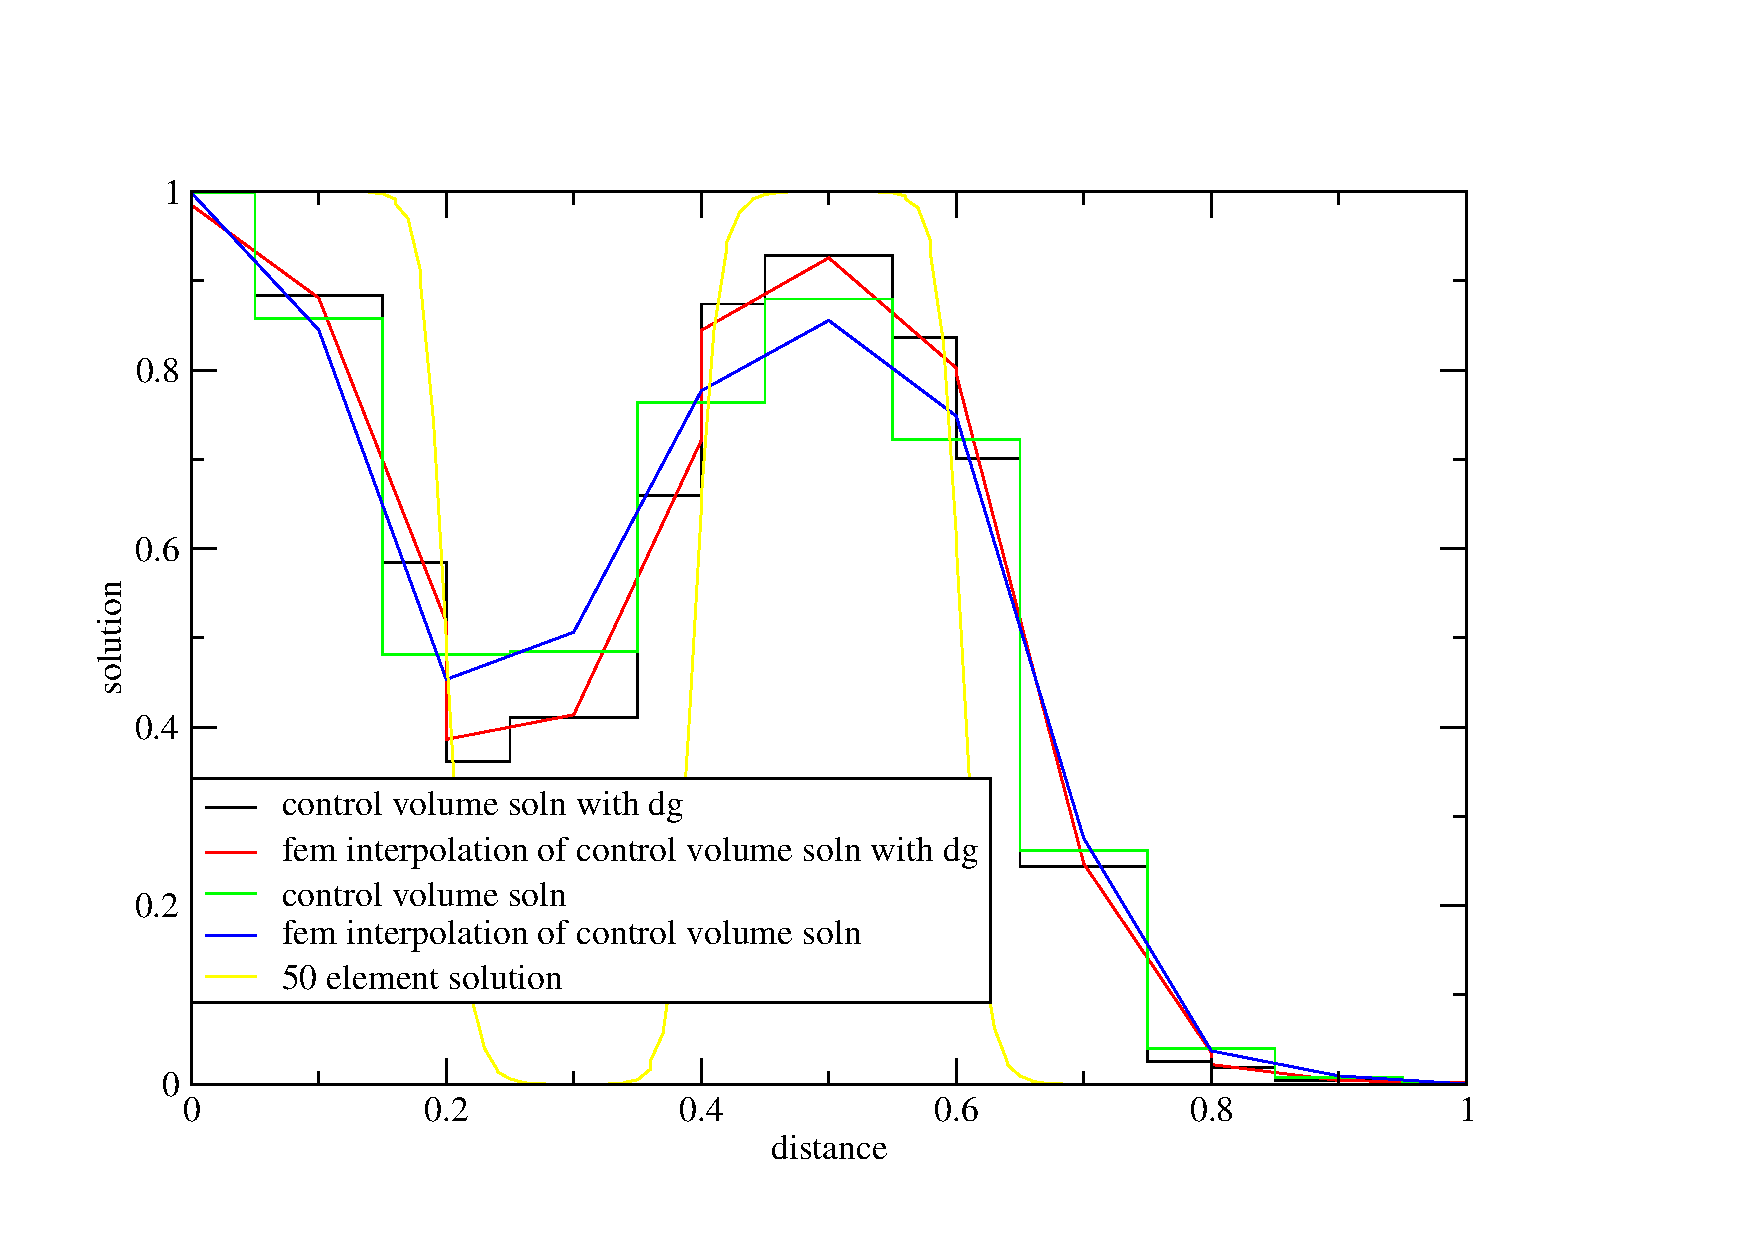
\includegraphics[width=17.5cm,height=12.5cm]{./doc_figures/compar-dg}
\end{center}
\vspace{0.cm}}
\caption{Comparison of discontinuous and continuous (between elements) 
control volume solution for a pure advection problem (from left to right) - 5 finite elements are used and the Courant number (based on the element width of 0.2) 
is 0.005. The solution has been advected a distance of 0.2 with 200 time steps. The 50 element solution is shown to give an indication of the accuracy of the solutions.}
\label{compar-dg}
\end{figure}





\begin{figure}[H]
\vbox{
\begin{center}
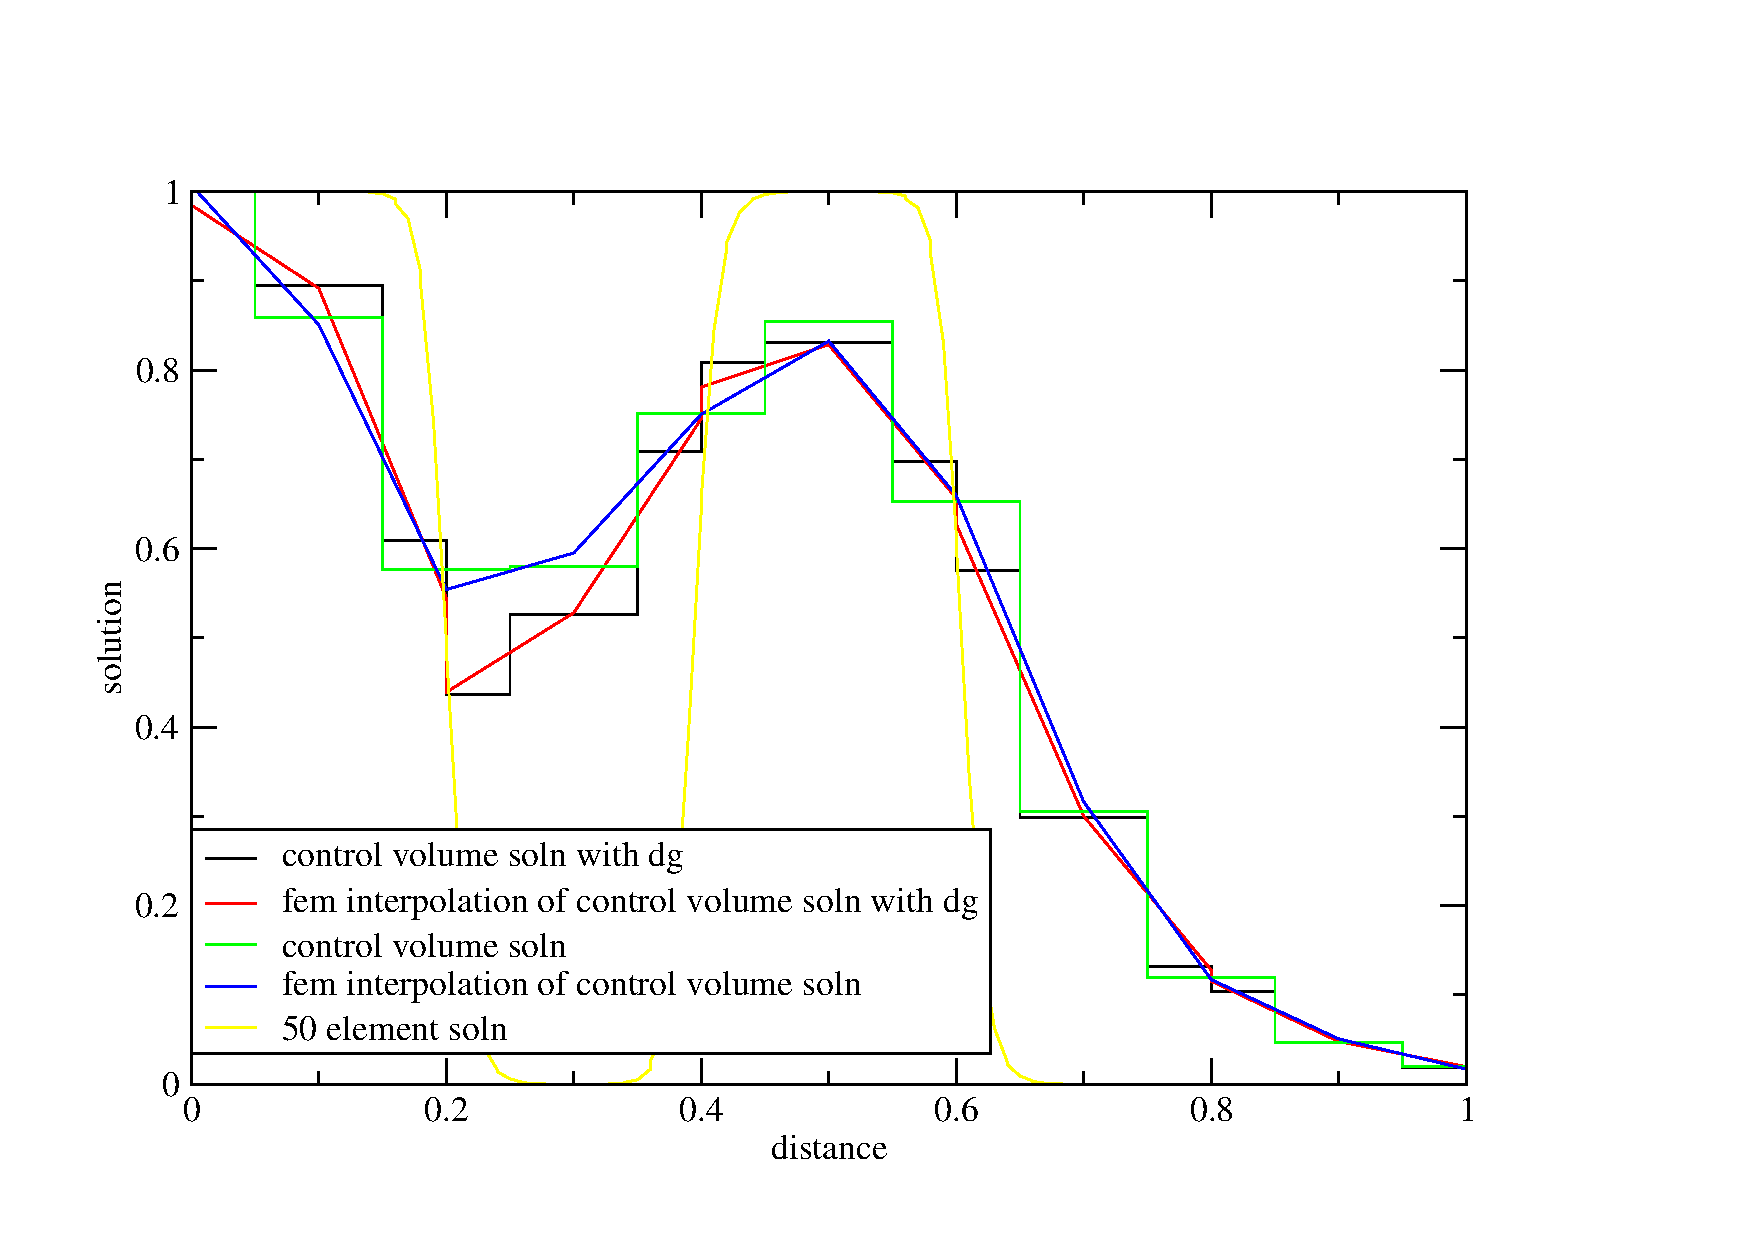
\includegraphics[width=17.5cm,height=12.5cm]{./doc_figures/compar-dg-bdt}
\end{center}
\vspace{0.cm}}
\caption{Comparison of discontinuous and continuous (between elements) 
control volume solution for a pure advection problem (from left to right) - 5 finite elements are used and the Courant number (based on the element width of 0.2) 
is 0.5 (2 based on the minimum width of a control volume). 
The solution has been advected a distance of 0.2 with 2 time steps. The 50 element solution is shown to give an indication of the accuracy of the solutions and has a Courant number (based on the element width) of 0.005. }
\label{compar-dg-bdt}
\end{figure}



\begin{figure}[H]
\vbox{
\begin{center}
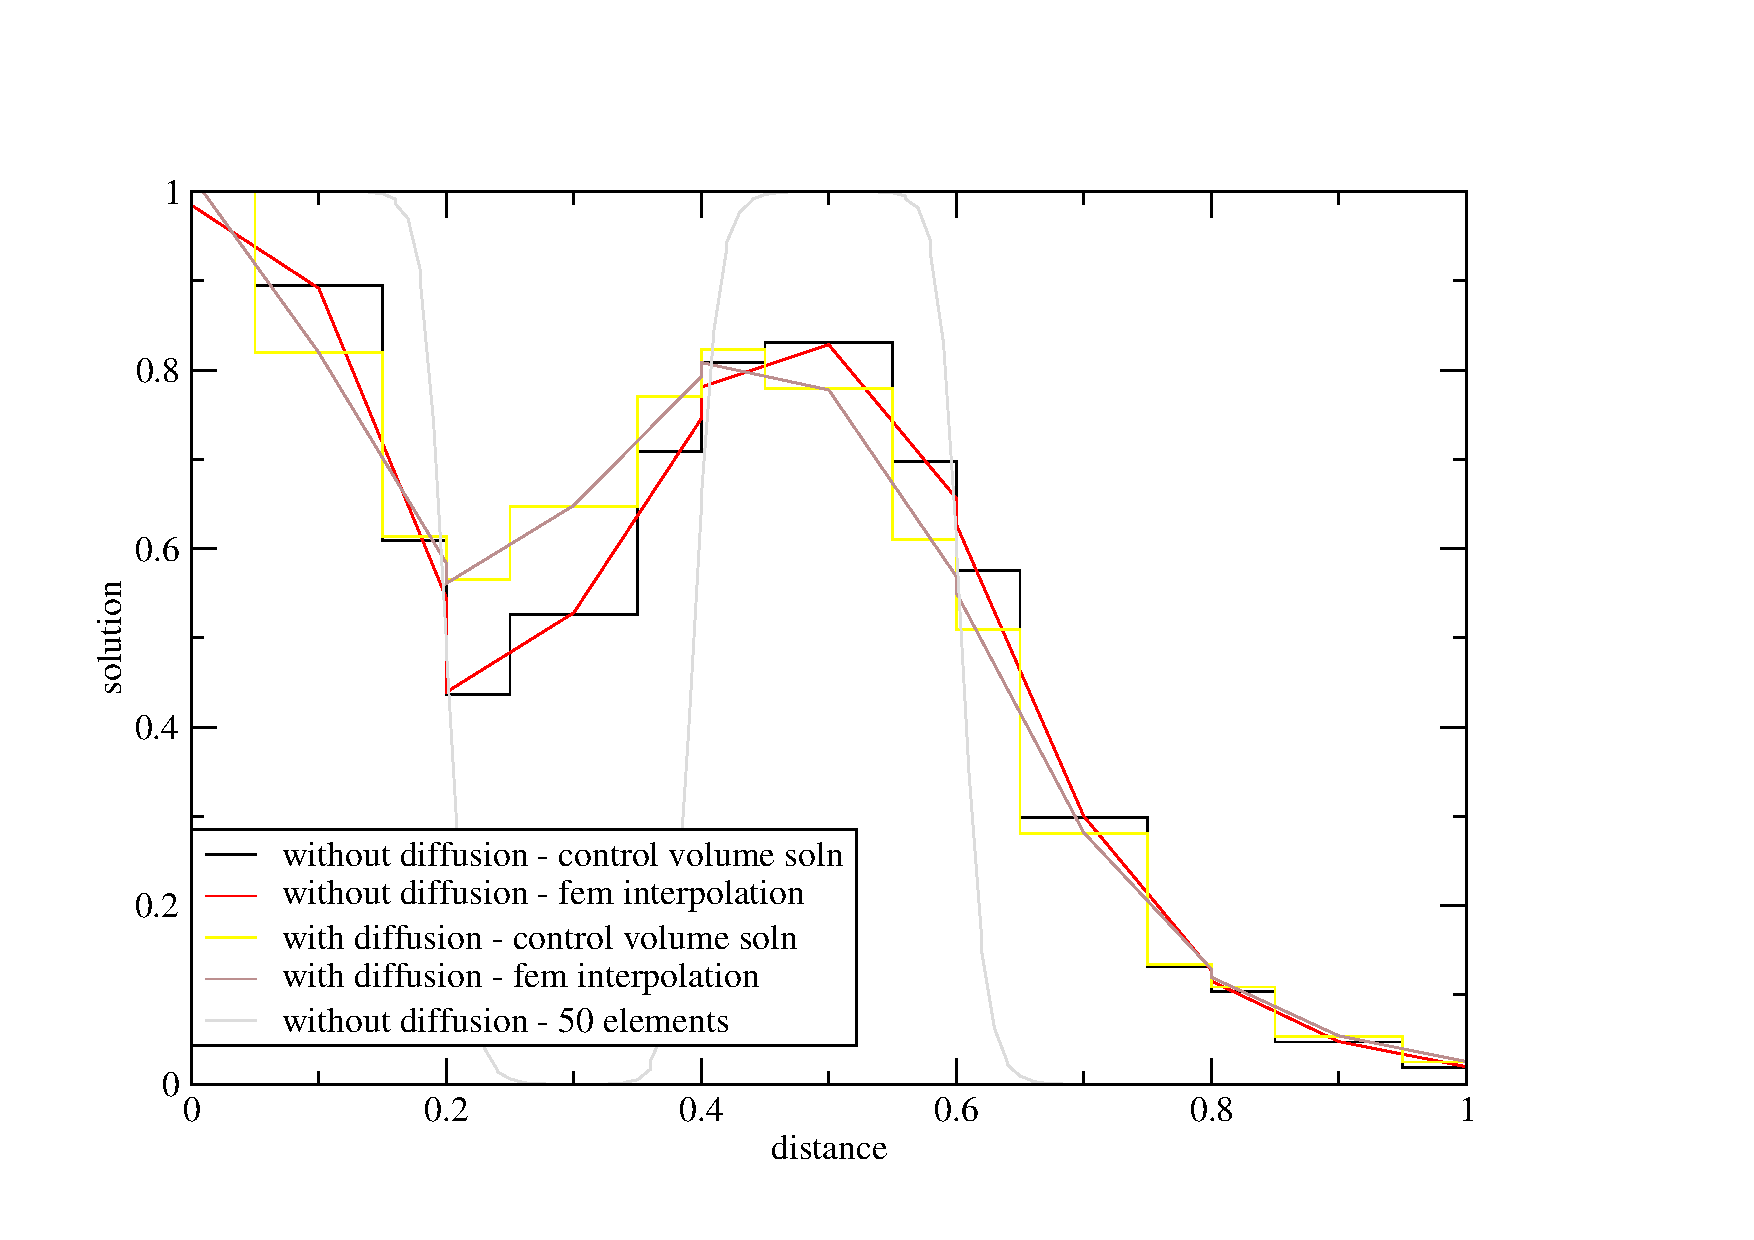
\includegraphics[width=17.5cm,height=12.5cm]{./doc_figures/compar-dg-bdt-diff}
\end{center}
\vspace{0.cm}}
\caption{The effect of diffusion using a discontinuous (between elements) 
control volume solution for an advection problem (from left to right) - 5 finite elements are used and the Courant number (based on the element width of 0.2) 
is 0.5 (2 based on the minimum width of a control volume). 
The solution has been advected a distance of 0.2 with 2 time steps. The 50 element solution is for pure advection and is shown to give an indication of the accuracy of the solutions and has a Courant number (based on the element width) of 0.005. }
\label{compar-dg-bdt-diff}
\end{figure}




\begin{figure}[H]
\vbox{
\begin{center}
\includegraphics[width=17.5cm,height=12.5cm]{./doc_figures/theta-bdt}
\end{center}
\vspace{0.cm}}
\caption{Value of the $\theta$ 'theta' time stepping parameter on the faces of the control volumes at the end of the 
simulation  - 5 finite elements are used and the Courant number (based on the element width of 0.2) 
is 0.5 (2 based on the minimum width of a control volume). 
The solution has been advected a distance of 0.2 with 2 time steps.  }
\label{theta-bdt}
\end{figure}


\begin{figure}[H]
\vbox{
\hbox{
\hspace{-1.cm}
\includegraphics[width=9.0cm,height=9.cm]{./doc_figures/converg-cv}
\hspace{-1.cm}
\includegraphics[width=9.0cm,height=9.cm]{./doc_figures/converg-fem}
}
\vspace{-0.cm}
\hbox{\hspace{4.cm}(a) \hspace{6.5cm}(b)}
\vspace{-0.cm}}
\label{converg}
\caption{Convergence of the solutions with discontinuity between elements and with increased resolution. A pure advection problem (from left to right) - the Courant number  
is 0.005. The solution has been advected a distance of 0.2. (a) the control volume solutions are shown. (b) the FEM interpolation of the control volume solutions are shown. }
\end{figure}


\begin{figure}[H]
\vbox{
\begin{center}
\includegraphics[width=17.5cm,height=12.5cm]{./doc_figures/converg-compare-fem}
\end{center}
\vspace{0.cm}}
\caption{Comparison of convergence of the solutions with and without discontinuity between elements and with an upwind and central difference flux between the elements and with increased resolution. A pure advection problem (from left to right) - the Courant number  
is 0.005. The solution has been advected a distance of 0.2. The FEM interpolation of the control volume solutions are shown.  }
\label{converg-compare-fem}
\end{figure}



\pagebreak

\cleardoublepage

%\part{Appendix}
\pagebreak
\begin{appendix}
%\input{code_user_guide}

\section{Buckley Leverett Equations with/without Gravity} 

\subsection{Nomenclature}
\begin{tabular}{c l}
%\hline
%
$f_{j}$: & fractional flow of phase $j$ \\
%
$f_{ij}$: & $\partial f_{i}/\partial S_{j}$ \\
%
$g$: & gravitational acceleration constant \\
%
$j$: & phase \\
%
$k$: & absolute permeability of the porous medium in 1D \\
%
$k_{rj}$:& relative permeability of phase $j$ \\
%
$k^{o}_{rj}$: & endpoint relative permeability of phase $j$ \\
%
$n_{j}$: & Corey exponent of phase $j$\\
%
$n_{p}$: & number of phases present\\
%
$S_{j}$: & saturation of phase $j$\\
%
$S_{j}^{\star}$: & normalized saturation of phase $j$\\
%
$S_{rj}$: & residual saturation of phase $j$\\
%
$v$: & flow velocity in 1D\\
%
$\mu_{j}$: & viscosity of phase $j$\\
%
$\rho_{mj}$: & mass density of phase $j$\\
%
$\lambda$: & eigenvalue (characteristic velocity)\\
%
$\Lambda$: & shock velocity\\
%
$\theta$: & dip angle of porous medium from horizontal\\
%
%\hline
\end{tabular}



\subsection{Equations}

Using the notation and derivation of \cite{Orr_2007}, the conservation equations for purely convective one-dimensional flow of two immiscible phases is

\begin{eqnarray}
&&\frac{{\partial S_j }}{{\partial \tau }} +  \frac{{\partial f_j }}{{\partial \xi }}  = 0 \label{eqn:BL}\\
&&j = g,w,o \nonumber
\end{eqnarray}

\noindent where dimensionless time $\tau = \frac{v t}{\phi L}$ and dimensionless distance $\xi = \frac{x}{L}$ .  For the two-phase water/gas system only one of these equations is independent as $S_g + S_w = 1$.  All variables are defined in the Nomenclature section.

The fractional flow of a component is defined as

\begin{eqnarray}
&&f_j = \frac{\frac{k_{rj}}{\mu_j}}{\sum_{n=1}^{n_p}{\frac{k_{rn}}{\mu_n}}} \left( 1-\frac{kg \sin \theta}{v} \sum_{n=1}^{n_p}{\frac{k_{rn}}{\mu_n}\left( \rho_{mj}-\rho_{mn} \right)} \right) \label{eqn:ff}
\end{eqnarray}

\noindent where

\begin{eqnarray}
&&k_{rj} = k_{rj}^o {\left(S_j^*\right)^{n_j}}\\
&&S_j^* = \frac{S_j - S_{rj}}{1-\sum_{n=1}^{n_p}{S_{rn}}} \nonumber
\end{eqnarray}

\noindent which can be written entirely in terms of $S_g$ for the Buckley-Leverett problem using $S_w = 1-S_g$.  Equation \ref{eqn:BL} can be solved as an eigenvalue problem by ...

The exact analytical form for the derivative of the fractional flow is

\begin{eqnarray}
\frac{df_g}{dS_g}&=& \frac{\left(\frac{\frac{d k_{rg}}{d S_g}}{\mu_g}\right) \frac{k_{rw}}{\mu_w}-\left(\frac{\frac{d k_{rw}}{d S_g}}{\mu_w}\right)\frac{k_{rg}}{\mu_g}}{\left(\frac{k_{rg}}{\mu_g}+\frac{k_{rw}}{\mu_w}\right)^2}\left( 1-\frac{kg \sin \theta}{v} \frac{k_{rw}}{\mu_w}\left( \rho_{mg}-\rho_{mw} \right) \right)\nonumber \\
&&-f_g\frac{kg \sin \theta}{v} \frac{\frac{d k_{rw}}{d S_g}}{\mu_w}\left(\rho_{mg}-\rho_{mw} \right)
\end{eqnarray}

\noindent where

\begin{eqnarray}
\frac{d k_{rg}}{d S_g} &=& k_{rg}^o n_g \frac{\left(S_g - S_{rg}\right)^{n_g-1}}{\left(1-S_{rg}-S_{rw}\right)^{n_g}}\nonumber \\
\frac{d k_{rw}}{d S_g}&=& -k_{rw}^o n_w \frac{\left(1-S_g - S_{rw}\right)^{n_w-1}}{\left(1-S_{rg}-S_{rw}\right)^{n_w}}\nonumber 
\end{eqnarray}



\subsection{Parameters in example problems}
All parameters in Equation \ref{eqn:BL} are assumed to be constant in the Buckley-Leverett problem.  The fractional flow parameters are given in Table \ref{table:paras}.

\begin{table}[h]
\begin{center}
\begin{tabular}{lrrrr}
\hline
Phase&$S_{rj}$&$k_{rj}^o$&$n_j$& $\mu_j$($cp$)\\
%%\lcline{1-1}\rlcline{2-5}
Gaseous&0.1&1.0&2.0&0.1\\
%Oleic&-&-&-&-\\
Aqueous&0.3&1.0&2.0&1.0\\
\hline
\end{tabular}
\caption{Fractional flow parameters for the benchmark Cases I-III.}
\label{table:paras}
\end{center}
\end{table}


\subsection{Solutions}

\subsubsection{Case I: Solution without gravity}
The first benchmark solution is for the case of no gravity, i.e. a horizontal displacement.  The initial (right state) and injection (left state) conditions are given in Table \ref{table:BCs}.

\begin{table}[h]
\begin{center}
\begin{tabular}{lrr}
\hline
BC & $S_g$ & $S_w$\\
%%\lcline{1-1}\rlcline{2-3}
Initial& 0.0 & 1.0\\
(right state)&  & \\
Injection&1.0 & 0.0\\
(left state)&  & \\
\hline
\end{tabular}
\caption{Boundary conditions for benchmark Cases I-III. }
\label{table:BCs}
\end{center}
\end{table}



\begin{figure}[h]
\centering
%\includegraphics[width=0.75\textwidth,viewport=10 10 420 420,clip]{./figures/BL_no_gravity}
\includegraphics[width=10.0cm,height=15.cm]{./figures/BL_no_gravity}
\vspace{-4.cm}
\caption{Top: Comparison the analytical solutions to Case I without gravity with the upstream weighted DG simulated solution with for 3 (green), 10 (blue) and 50 (red) grid blocks.  Bottom: Comparison the analytical solutions to Case I without gravity with the mixed weighted DG simulated solution for 3 (green), 10 (blue) and 50 (red) grid blocks.} 
\label{fig:BL_no_grav}
\end{figure}


The displacement consists of a fast moving shock wave from the initial condition, with no gas, to a gas saturation of $S_g = 0.3255$, followed by a rarefaction wave to the residual water saturation. As there is no transfer of components between phases, it is impossible to move the residual water from the system.

The DG simulator was run in 2 modes, upstream weighting and 80\% upstream weighting.  A comparison of the analytical solution for various levels of refinement is shown for upstream weighting on the top of Figure \ref{fig:BL_no_grav} and for mixed weighting on the bottom. 

\paragraph{Displacements with gravity}

In this case the flux in the conservation law is slightly different.  The fractional flow curve as computed from Eq. \ref{eqn:ff} may be larger than one or less than zero, which is physically meaningless in one dimension as $f_g$ is defined as the fraction of the total flow that is taken up by the gas phase.  The impossible fluxes are caused by the inability of a 1D model to capture counter-current gravity-driven flow.  A 2D benchmark case to study this effect will be dealt with later.  Anytime Eq. \ref{eqn:ff} gives $f_g > 1.0$ it must be that in 1D $f_g = 1.0$, similarly if $f_g < 0.0$ in Eq. \ref{eqn:ff}, $f_g = 0.0$.  The additional parameters necessary for the cases including gravity are in Table \ref{table:grav_const}.  The phase densities are calculated using the method from \cite{spycher_2003}.


\begin{table}[h]
\begin{center}
\begin{tabular}{lr}
\hline
$\rho_g$ ($\frac{kg}{m^3}$)& 710 \\
%$\rho_o$ ($\frac{kg}{m^3}$)&-\\
$\rho_w$ ($\frac{kg}{m^3}$)& 1050\\
g ($\frac{m^2}{s}$)& 9.8 \\
k ($ m^2$)& $9.87E-13$\\
v ($ \frac{m}{s}$)& $5.00E-06$\\
\hline
Case II &\\
$\theta$ (degrees) & -90 \\
\hline
Case III &\\
$\theta$  (degrees)& 90  \\
\hline
\end{tabular}
\caption{Additional parameters needed for benchmark Cases II and III with gravity. Phase densities for water and super-critical CO$_2$ are at 80$^oC$ and 27$MPa$. }
\label{table:grav_const}
\end{center}
\end{table}



\paragraph{Case II: Displacements with gravity slowing displacement}

The first benchmark solution including gravity is the injection of oil into the bottom of a vertical core or sand pack. In this case analytical solution in the presence of gravity is physically meaningful, though there is a small region at low $S_g$ where $f_g < 0.0$.  The solution structure is the same as in the displacement without gravity.  Because the more dense oil is being pushed into the core against the force of gravity the leading shock front and rarefaction wave have both slowed down substantially.


\begin{figure}[h]
\vspace{-1cm}
\centering
\includegraphics[width=15.0cm,height=20.cm]{./figures/BL_gravity_up}
%\includegraphics[width=0.75\textwidth,viewport=10 0 390 300,clip]{./figures/BL_gravity_up}
\vspace{-5.5cm}
\caption{Analytical solution to Case II, the stable benchmark case with gravity (black) slowing the displacement.  A fine-grid FD solution (red) and the analytical solution for the case without gravity (blue) are shown for comparison purposes.} 
\label{fig:BL_grav_up}
\end{figure}

\paragraph{Case III: Displacements with gravity accelerating displacement}

The second benchmark solution including gravity is the injection of oil into the top of a vertical core or sand pack. In reality this displacement is gravity unstable and needs to be modelled in two-dimensions, but for the purposes of benchmarking the code it is still useful. 

The solution with gravity is a shock wave from the right state to the saturation $S_g = 0.2960$ followed by a rarefaction wave to $S_g = 0.3340$.  Then there is a constant state to the injection composition.  This constant state is caused by the fact that $f_g > 1.0$ for large gas saturations and no longer tapers off uniformly as the residual water saturation is approached.

The analytical solution with gravity is shown in Figure \ref{fig:BL_grav_down} with a fine-grid FD solution and the analytical solution without gravity for comparison.  

\begin{figure}[h]
\vspace{-1cm}
\centering
\includegraphics[width=15.0cm,height=20.cm]{./figures/BL_gravity_down}
\vspace{-5.5cm}
%\includegraphics[width=0.75\textwidth,viewport=10 0 390 300,clip]{./figures/BL_gravity_down}
\caption{Analytical solution to Case III, the unstable benchmark case with gravity (black) accelerating the displacement.  A fine-grid FD solution (red) and the analytical solution for the case without gravity (blue) are shown for comparison purposes.} 
\label{fig:BL_grav_down}
\end{figure}


\end{appendix}

\cleardoublepage

\pagebreak
\bibliography{QCCSRC_bib}
\bibliographystyle{unsrt}

\cleardoublepage
\phantomsection
\renewcommand\leftmark{}
\renewcommand\rightmark{Index}
\addcontentsline{toc}{chapter}{Index}

\printindex


\end{document}
